%-----------------------------------------------------------------------------------------------------------------%
%\documentclass[10pt,compress,handout]{beamer}             %For printable version
\documentclass[10pt,compress,xcolor=dvipsnames,aspectratio=169]{beamer}    %For presentation version
%\setbeameroption{show notes}
%\setbeamercovered{transparent}

%% ----- Theme for projector display version --------------
\mode<presentation> {
%    \usetheme{Warsaw} %standard topbars
%    \usetheme{Berlin} %
%    \usetheme{Goettingen} %side bars
%NONE: %cleaner and more space

      \definecolor{Verde}{RGB}{05,130,25}
      \definecolor{Verde2}{RGB}{34,139,34}
	  \definecolor{mygreen}{RGB}{0,73,44}

%    \usecolortheme{dolphin}
%    \usecolortheme{beaver}f

%    \usecolortheme{seahorse}  %%bars at the top
%    \setbeamercolor{structure}{fg=Verde, bg=Verde}

%    \usecolortheme[named=Green]{structure}
%    \usecolortheme[named=ForestGreen]{structure}
%    \usecolortheme[named=OliveGreen]{structure}
    \usecolortheme[named=Verde]{structure}

    %\useinnertheme{circles} %%must use \usepackage{textcomp} otherwise Latex Warning
    \useinnertheme{rounded} %%rectangles, circles, rounded, inmargin,
    \useoutertheme{split} %%puts sections on the upper-left hand side and subsections in upper-rhs; name and title on the lower (watch out for page nums)

%    \setbeamercolor*{palette primary}{use=structure,fg=white,bg=Verde}    %%upper and lower right hs
%    \setbeamercolor*{palette secondary}{use=structure,fg=black,bg=Verde}
%    \setbeamercolor*{palette tertiary}{use=structure,fg=black,bg=blue}
%    \setbeamercolor*{palette quaternary}{use=structure,fg=black,bg=Verde}   %%upper and lower left hs

\setbeamertemplate{navigation symbols}{}  %%Get rid of the navigation symbols at the bottom
\setbeamertemplate{footline}[page number]{} %%Show the page number at the bottom of the slides instead of name and title
%\setbeamertemplate{footline}[frame number]{} %%Show the frame number (not counting pauses) at the bottom of the slides instead of name and title
%\setbeamertemplate{footline}[text line]{\parbox{\linewidth}{\vspace*{-8pt}\insertshortauthor  \hfill  \insertpagenumber }} %/ \insertpresentationendpage

}  %%END OF MODE PRESENTATION

%% -------------- Packages ------------------------------ %%
%\pdfoptionpdfminorversion=6 %some attachments are PDF version 1.6 and I get an error
\usepackage[english]{babel}

\usepackage{amsfonts}
\usepackage{amsmath}
\usepackage{amssymb}
\usepackage{amsthm}
\usepackage{mathtools}
\usepackage{graphicx}
\graphicspath{{./include/}}% where figures are saved  %%must \usepackage{graphicx}
\usepackage{comment,footmisc,pdflscape,array,booktabs}
\usepackage{threeparttable}
\usepackage{balance}
\usepackage{lettrine}
\usepackage{type1cm}
%\usepackage{subfigure}
\usepackage{bbm}
\usepackage{multirow}
\usepackage{chngcntr}
\usepackage{multicol}
\usepackage{xr}
\usepackage{ulem}
\usepackage{color}
\usepackage{wrapfig}
\usepackage{tabularx}
\usepackage{booktabs}
\usepackage{dcolumn}

%\usepackage{color}
%\usepackage{booktabs}
\usepackage{hyperref}
%\usepackage{multimedia}
%\usepackage{animate}
\usepackage{multirow}
\usepackage{multicol}
\usepackage{bigstrut} %creates some space next to lines in table to improve appearance
\usepackage{rotating}
\usepackage{setspace}
%\usepackage{caption} %captions for the figures
\usepackage{subcaption} %allows subfigures and subcaptions
\captionsetup{compatibility=false}
\usepackage{url}
\usepackage{lmodern}  %%allowing font sizes at arbitrary sizes // removes LaTeX Font Warning: Font shape `OT1/cmss/m/n' in size <4> not available

%\usetikzlibrary{shapes,arrows,trees,snakes,positioning,fit,shadows}
\renewcommand\textbullet{\ensuremath{\bullet}}

% counter for examples
\newcounter{ex}
\setcounter{ex}{1}
\newcommand{\nbex}{\arabic{ex}\addtocounter{ex}{1}}

%figures
\renewcommand{\figurename}{Figure~\arabic{figure}}
\renewcommand{\tablename}{Table~\arabic{table}}

% math symbols
\newcommand{\Nor}[2]{N\!\left(#1, #2\right)}    	% normal distribution
\newcommand{\indp}{\perp\!\!\!\perp} 			% independence
\newcommand{\1}[1]{\mathrm{1\hspace*{-2.5pt}l}[#1]}	% indicator
\newcommand{\Var}{\mathrm{Var}}
\newcommand{\Cov}{\mathrm{Cov}}
\newcommand{\Expect}{{\rm I\kern-.3em E}}

\DeclareMathOperator{\exer}{\mathnormal{E}} %exercise


%% ----- The next 3 lines allow natbib to work properly in a Beamer Document --
\makeatletter
\def\newblock{\beamer@[EMAIL PROTECTED]}
\makeatother

%%------ New commands ---- %%
\newcommand\FontTwelve{\fontsize{12}{7.2}\selectfont} %%Reduces the font sizes of one slide only. FontSize=10, Baselineskyp=7.2
\newcommand\FontTen{\fontsize{10}{7.2}\selectfont} %%Reduces the font sizes of one slide only. FontSize=10, Baselineskyp=7.2
\newcommand\FontEight{\fontsize{8}{7.2}\selectfont} %%Reduces the font sizes of one slide only.
\newcommand\FontSix{\fontsize{6}{7.2}\selectfont} %%Reduces the font sizes of one slide only.

\hypersetup{
   colorlinks = true,
   citecolor = {Verde},
   linkcolor = {Verde},
   menucolor = {Verde},
   filecolor = {Verde},
 }


%%%%%%%%%%%%%%%%%%%%%%%%%%%%%%%%%% TITLE %%%%%%%%%%%%%%%%%%%%%%%%%%%
%\title[GxE Smoking]{\textbf{Health Behaviors, Genetics, and the Environment}}
%\author[Pietro]{Pietro Biroli}
\title[GxInsurance]{
%\textbf{Genetics and Health Insurance: How Genes and Insurance Status Affect Smoking Decisions after Health Shocks}
\textbf{Moral Hazard Heterogeneity: \\ Genes and Health Insurance Influence Smoking after a Health Shock}
}
\author[Pietro, Laura]{
Pietro Biroli and Laura Zwyssig
\\ \medskip {\scriptsize thanks to GEIGHEI team, Regina Seibel, and Pia Arce}
}%end author
\institute[UZH]{University of Z\"urich}
\date{{\color{blue} University of Connecticut} \\ {\color{Verde} March 8th, 2021}}


\begin{document}

%------------------------------------------------------------------------%
\frame{\titlepage}

\AtBeginSection[]{\frame<beamer>{\frametitle{Outline}\tableofcontents[currentsection]}}
\AtBeginSubsection[]{\frame<beamer>{\frametitle{Outline}\tableofcontents[currentsubsection]}}

%\frame{\frametitle{Outline}\tableofcontents}

%%------------------------------------------------------------------------%
%%% INTRODUCTION %
%%------------------------------------------------------------------------%
\section{Research Question}

%\begin{block}{Research Question}
%Does genetic predisposition to health behaviors shape our response to shocks and the environment?
%\end{block}
%
%\begin{itemize}
%	\item Aim  = use genetics to understand health behaviors:
%	\[ H = f(G,E) \]
%	\item Enrich econ with genetic heterogeneity
%\end{itemize}

%--------------------------------------------------------------%
\begin{frame}
\frametitle{Genes, health insurance, smoking choices}

%%%What is the question I want to answer?
\textbf{What}:
	\begin{itemize}
		\item[$Agenda:$] Use genes to assess individual level heterogeneity in economic parameters
		\item[$Paper:$] Does reaction to a negative health shock depend on health insurance and genetic differences?
	\end{itemize}

  \vspace{2ex}
  \pause

%%%How do I answer the question
\textbf{How}:
\begin{itemize}
  \item Focus on smoking behavior following a cardio-vascular health shock
  \item Identification: US adults who receive free health insurance coverage after 65 (Medicare)
  \item Compare high and low genetic predisposition to smoking (G$\times$E)
\end{itemize}

  \vspace{2ex}
  \pause

%%%Why do we care?
\textbf{Why}:
\begin{itemize}
		\item Interplay between financial and biological constraints:
		\begin{itemize}
			\item Health insurance buffers financial consequences of health shocks
			\item Genetic predispositions influence behavioral responses
		\end{itemize}
%		\item Use genes to better understand health choices
%		\begin{itemize}
			\item Understand \textbf{heterogeneity in moral hazard}
%		\end{itemize}
%		\item Individualized health insurance profiles?
\end{itemize}
\end{frame}

%--------------------------------------------------------------%
\begin{frame}{Preview}

\begin{itemize}
	\item Identification assumptions:
	\begin{itemize}
		\item Probability of health shock increases with age ...
		\item ... but \emph{no jump} at 65
	\end{itemize}

	\vspace{3ex}

	\item Results:
	\begin{itemize}
		\item Health shock when uninsured $\Rightarrow$ less smoking...
		\item ... but \textit{only} for low PGS.
		\item G$\times$E effect size: 27.9 pp
	\end{itemize}
\end{itemize}

\end{frame}

%%=================================================================================

\begin{frame}{Why should we care?}\label{frame:why}

\begin{itemize}
\item Genes cannot be changed ...
\item ... but \textbf{environment} can!
\item Interplay between genes (bio) and environment (econ) is essentially everywhere \cite{Rutter2006}

\vspace{3ex}

\item Understand differential effects of genetic predisposition based on environment (G$\times$E)
\begin{enumerate}
	\item[--] shed light on pathways and mechanisms
	\item[--] provide measure of essential heterogeneity
	\item[--] revisit old econ concept with new lens
\end{enumerate}

\vspace{3ex}

\item Empirics: genes are cheaper to measure and more and more available  \hyperlink{frame:dollargenome}{\beamergotobutton{}}
\item Theory: biologically founded model
\item Policy: understand sources of heterogeneity and discuss \textit{fairness}
\item Individual: choose individualized intervention
%Use theory to think through issues of causality, make predictions, and guide understanding
%%aimed at understanding the various causal pathways and mechanisms

\end{itemize}
\end{frame}

%%=================================================================================
%\begin{frame}
%\frametitle{Related Literature}
%\begin{footnotesize}
%\begin{enumerate}
%
%	\item Nature and Nurture (Twin Studies):
%			Use MZ/DZ twins to estimate genetic and environmental heritability. \\ {\footnotesize See \cite{Galton1874,Taubman1976,Kohler2011}} %Behrman1989,Plomin1977,Purcell2002,
%	%\item<2->[$\hookrightarrow$] {\textbf{Contribution}}: Specific biological mechanisms interacting with environment
%
%	\vspace{2ex}

%	\item G $\times$ E:
%			Use molecular genetics and measures environment and investigate their interplay. \\ {\footnotesize See \cite{Caspi2002,Fletcher2012,Barcellos2018,Belsky2018mobility,Schmitz2017,Schmitz2017vietnam,Wedow2018}. %Murcray2009,Young2016
%	%\item<2->[$\hookrightarrow$] {\textbf{Contribution}}: Specific biological mechanisms interacting with environment
%
%	\vspace{2ex}
%
%	\item Genoeconomics:
%			Find genetic determinants of economic behaviors: risk aversion, time and social pref., addiction. \\ {\footnotesize See \cite{Benjamin2007,Cesarini2009,Benjamin2014}}%Cesarini2010,Ebstein2010,Benjamin2011,Benjamin2012,
%
%	%\item<2->[$\hookrightarrow$] {\textbf{Contribution}}: genes as a channel mediating SES
%
%	\vspace{2ex}
%
%	\item Mendelian Randomization:
%			Genes as IV  \\ {\footnotesize See \cite{DaveySmith2003,Fletcher2009,VonHinkeKesslerScholder2016,Cawley2011}} %Ebrahim2008,Palmer2011,DaveySmith2011,VonHinkeKesslerScholder2011a,Fang2013,
%
%	\item<2->[$\hookrightarrow$] {\textbf{Contribution}}: Discuss its validity

%	\vspace{2ex}
%
%	\item Healthy behaviors: Connection between health, health behaviors, addiction, income \\ {\footnotesize See \cite{Grossman1972,Becker1988,Lakdawalla2005,Galama2015theory,Scholz2013}} %Grossman2000,Dustmann2000,
%	%\item<2->[$\hookrightarrow$] {\textbf{Contribution}}: introduce genetic heterogeneity in the model
%
%\end{enumerate}
%\end{footnotesize}
%\end{frame}
%

%--------------------------------------------------------------%
\begin{frame}
\frametitle{Previous work:}
\begin{itemize}
	 \item Smoking increases diseases and health-care costs (400k deaths, \$300 billion per year in US) {\scriptsize \cite{USDHHS2014,Goodchild2017,Ma2018,Xu2015}}

	 \smallskip

	 \item Severe health shocks reduce smoking {\scriptsize \cite{Clark2002,Falba2005,Khwaja2006learn,Keenan2009,Sundmacher2012}}

	 \smallskip
%	 \item Reduction depends on expected benefit vs. financial cost {\scriptsize \cite{Richards2014}}
%	 \smallskip

	 \item Health insurance plays a big role (moral hazard) {\scriptsize \cite{Richards2014,Marti2017,Einav2013,Einav2018}}

		\smallskip

	 	\item G $\times$ E:
			Use molecular genetics and measures of the environment and investigate their interplay. \\ {\footnotesize See \cite{Caspi2002,Barcellos2018,Belsky2018mobility,Rimfeld2018,Schmitz2017,Schmitz2017vietnam, Rosenquist2015}} %Murcray2009,Young2016

	\smallskip

	\item Genoeconomics:
			Find genetic determinants of economic behaviors: risk aversion, time and social pref., addiction. \\ {\footnotesize See \cite{Benjamin2007,Cesarini2009,Benjamin2014}}%Cesarini2010,Ebstein2010,Benjamin2011,Benjamin2012,

	\smallskip
	\pause
	\item[$\hookrightarrow$] \textbf{Contribution}: leverage genetic variants to measure heterogeneity in moral hazard

\end{itemize}
\end{frame}

\section{Genes for Econ}

%=================================================================================

\begin{frame}{Genetics for social scientists} \label{frame:genetics}

    \begin{minipage}{.7\textwidth}
\begin{itemize}
	\item Human genome: series of 3 billion letter pairs (A,G,T,C)
	\item Genetic variants: one-letter changes across individuals (single nucleotide polymorphisms, SNPs)
	\item About $\approx 10$m SNPs \cite{1000Genomes2015}
	\item Genome-wide association studies (GWAS) have identified genome-wide significant relationships between specific SNPs and health behaviors
	\item We use SNPs identified from large, replicated GWAS to create summarized genetic scores to study gene-by-SES interplay \hyperlink{fig:manhattan2}{\beamergotobutton{hits}}
\end{itemize}
    \end{minipage}
    \begin{minipage}{.2\textwidth}
      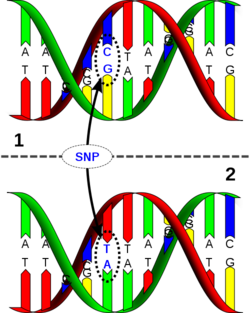
\includegraphics[scale=0.4]{SNP2}
    \end{minipage}

\end{frame}


%=================================================================================

\begin{frame}{PolyGenic Scores (PGS)}
Discovery stage:
		\vspace{-0.7cm}
\begin{columns}[T]
	\begin{column}{0\textwidth}
	\end{column}%
	\hfill%
	\begin{column}{.2\textwidth}
		\vspace{2cm}
		GWAS {\color{Verde}\cite{GSCAN2019gwas}}
	\end{column}%
	\hfill%
	\begin{column}{.8\textwidth}
		\begin{figure}
		\centering
		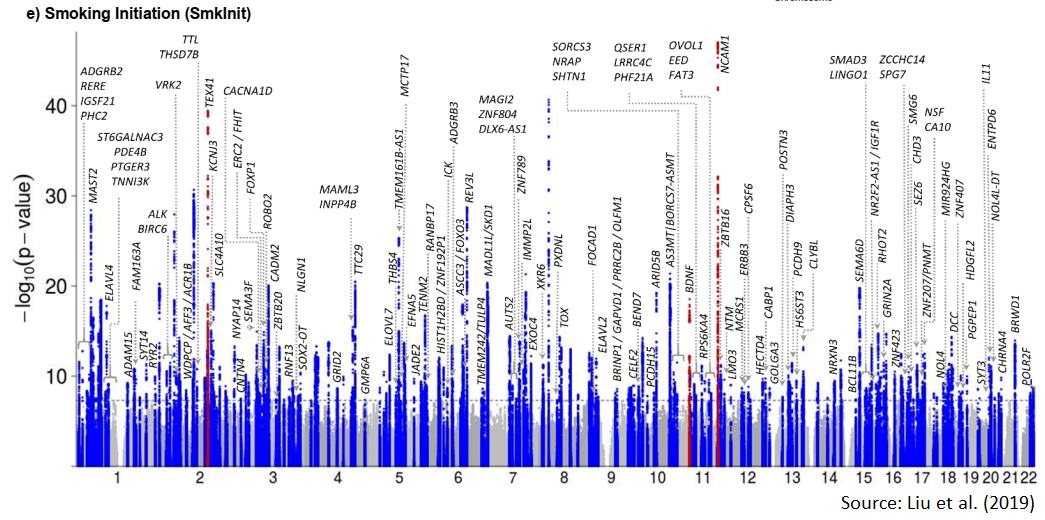
\includegraphics[width=0.9\textwidth]{./include/smokeInit_manhattan.png}
		\label{fig:manhattan}
		\end{figure}
	\end{column}%
\end{columns}

Prediction stage:
\begin{columns}[T] % align columns
	\begin{column}{.03\textwidth}
	\end{column}%
	\hfill%
	\begin{column}{.2\textwidth}
		\vspace{-0.45cm}
		{\color{Verde}\begin{align*}
			PGS_i = \sum_{j=1}^{J} W_j G_{ij},
		\end{align*}}
	\end{column}%
	\hfill%
	\begin{column}{.77\textwidth}
		\begin{footnotesize}
where $G_{ij}$ is the genotype for individual $i$ at SNP $j$, and the weight $W_j$ is the OLS association between SNP $j$ and outcome. Normalized to have mean zero and standard deviation one.
		\end{footnotesize}
	\end{column}%
\end{columns}

\end{frame}

%%=================================================================================
%
%\begin{frame}{Polygenic Scores}
%Construct index of genetic propensity for trait $Y$:
%
%\begin{align}
%PGS_i = \sum_{j=1}^{J} W_j G_{ij},
%\end{align}
%
%where $G_{ij}$ is the genotype for individual $i$ at SNP $j$, and the weight $W_j$ is the OLS association between SNP $j$ and outcome $Y$.
%
%Normalized to have mean zero and standard deviation one.
%
%\begin{figure}[hbtp]
%\centering
%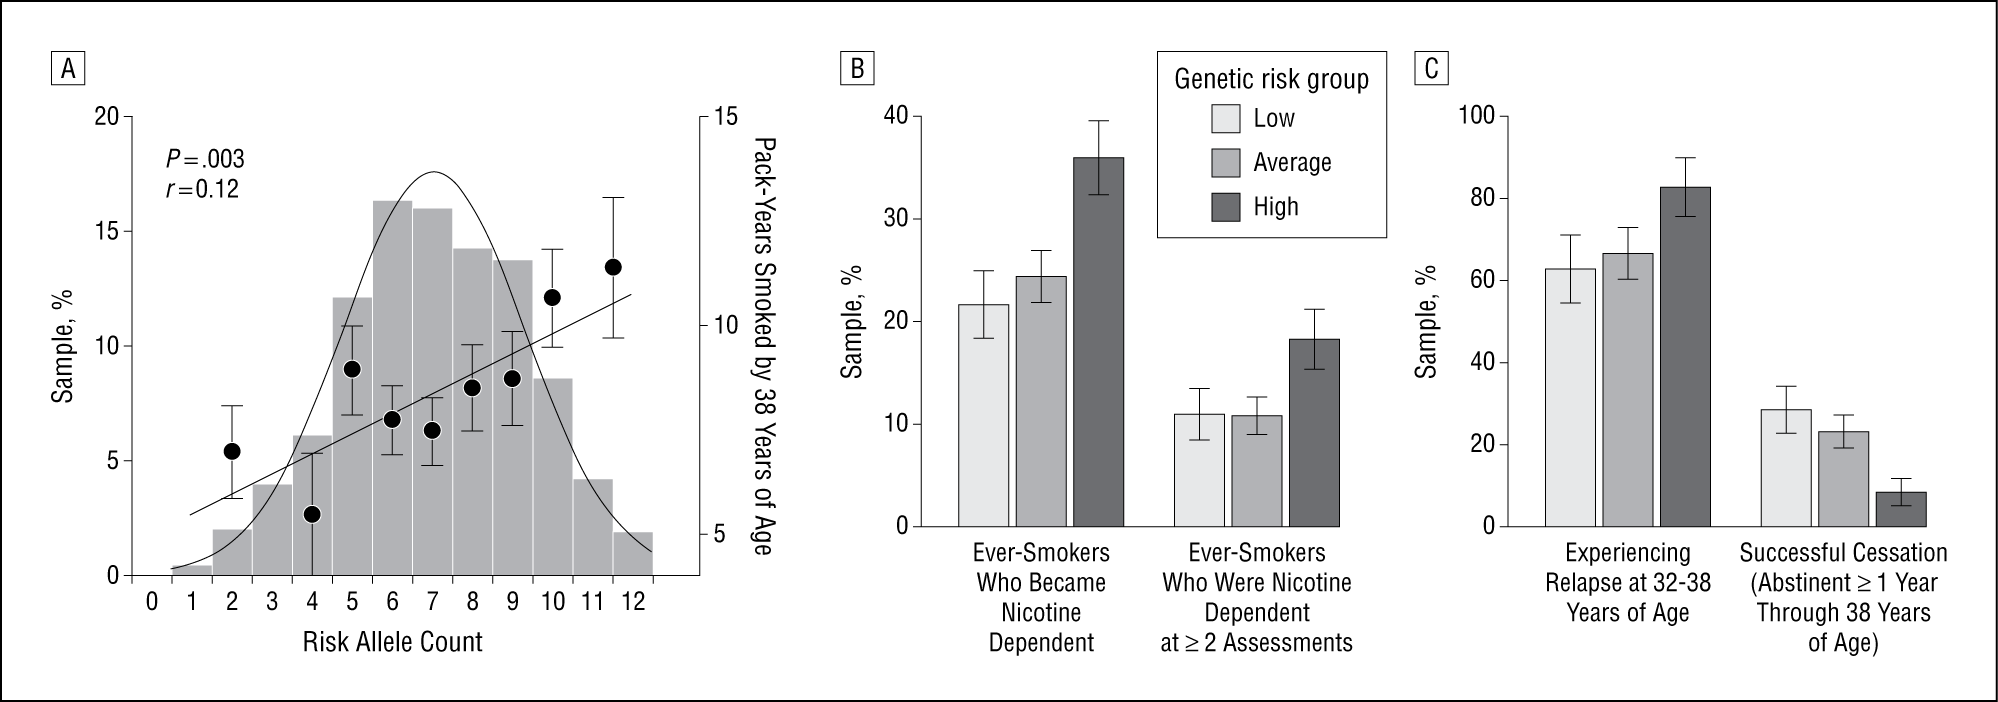
\includegraphics[height=0.3\textheight]{Belsky2013smokingPGS}
%\end{figure}
%
%\cite{Belsky2013smoke}
%
%\end{frame}

%=================================================================================

\begin{frame}{Polygenic Scores}
In our setting \\
Data = Health and Retirement Study \\
Y = Pr(Smoking) \\
$W_j$ = taken from \cite{GSCAN2019gwas}

\begin{figure}[hbtp]
\centering
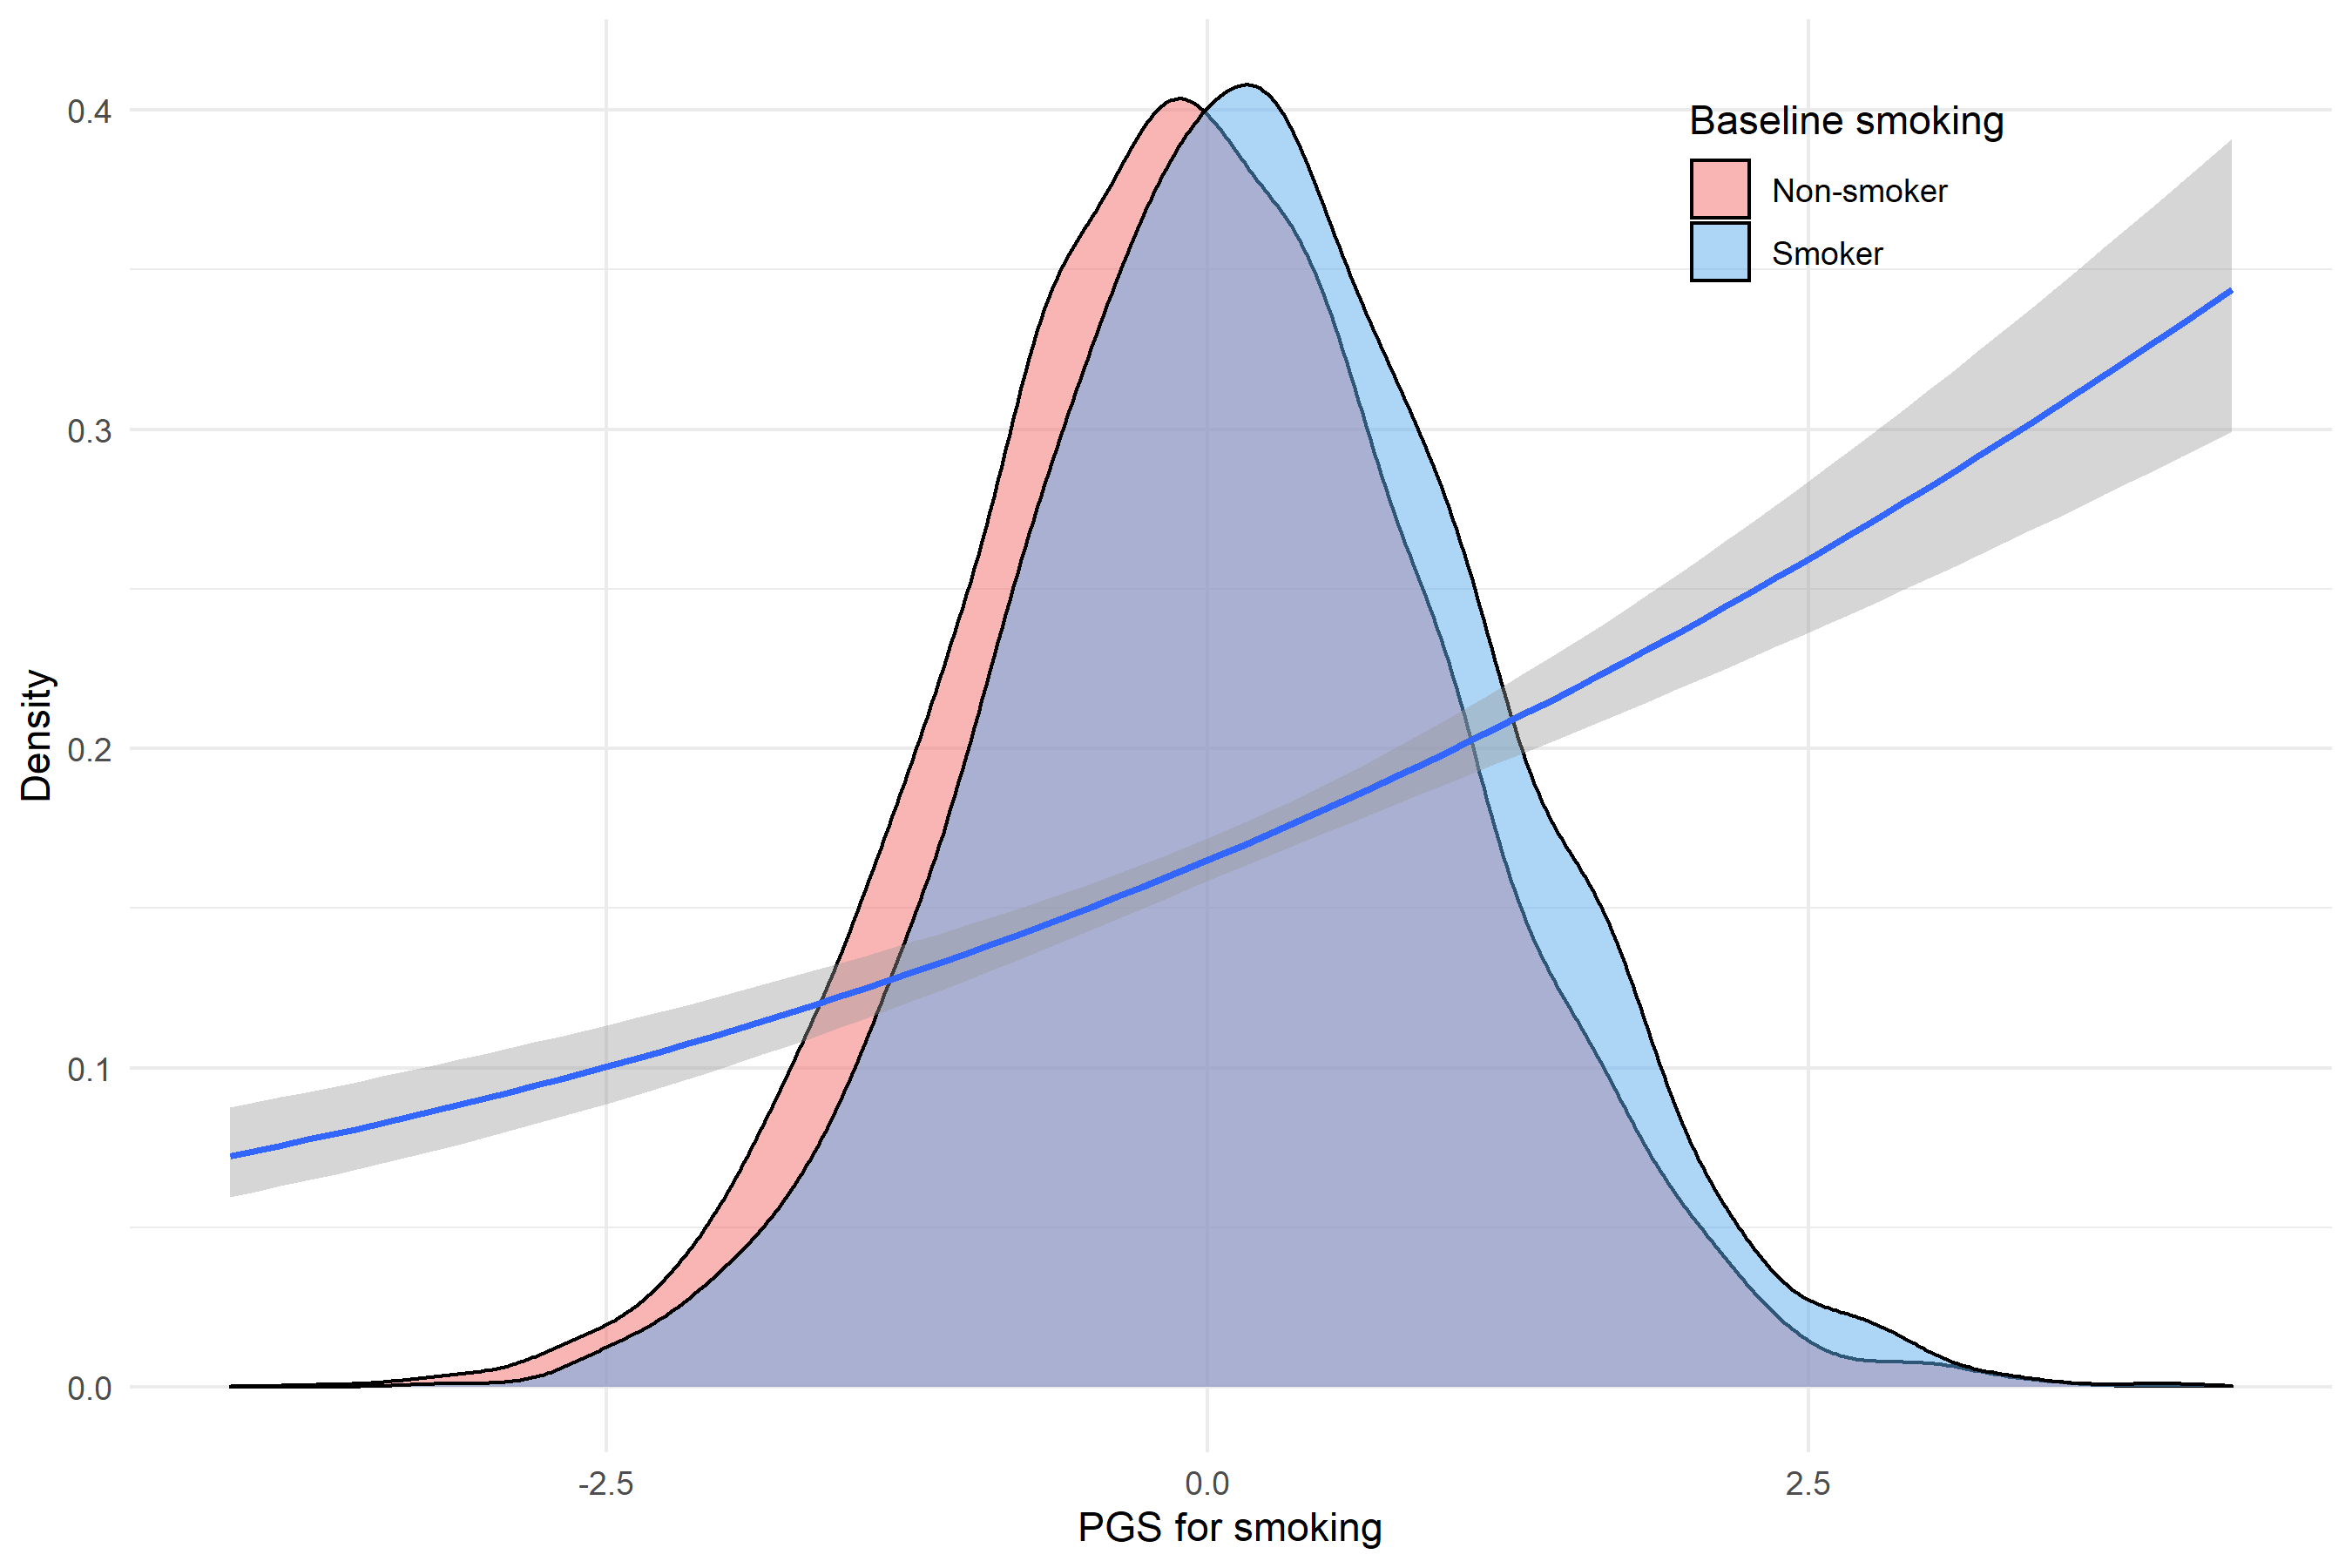
\includegraphics[height=0.7\textheight]{../../3_output/make_histograms/pgs_density_6070_smoken_smooth.png}
\end{figure}

\end{frame}

%--------------------------------------------------------------%
\section{Empirical Analysis}
\subsection{Data and setting}
%--------------------------------------------------------------%
\begin{frame}
\frametitle{Data}%{Analytic Sample}

\begin{itemize}
	\item Use HRS data: US-representative survey of 50+ (1992-2016)
	\item Final sample size = $26,022$ obs from $5,854$ individuals
	\begin{itemize}
		\item Ever smoked $\geq 100$ cigarettes (at baseline)
		\item Ages: 60-70
		\item Observed at least 2 waves
		\item European descendants
		\item Non-missing smoking, PGS, insurance, health shock
	\end{itemize}
\end{itemize}

\end{frame}


%--------------------------------------------------------------%
\begin{frame}\frametitle{Variables} \label{frame:vars}

\begin{itemize}
	\item Outcome \textit{\color{Verde} Y} = current smoking status $\in \{0,1\}$
	\begin{itemize}
		\item Self reported
	\end{itemize}

	\smallskip

	\item High PGS \textit{\color{Verde} g} = above 33$^{rd}$ in PGS for smoking initiation
	\begin{itemize}
		\item Use \cite{GSCAN2019gwas} for weights
	\end{itemize}

	\smallskip

	\item Health {\color{Verde} shock} = first diagnosis of acute cardiovascular condition
	\begin{itemize}
		\item Heart problem: heart attack, coronary heart disease, angina, congestive heart
failure, or other heart problems
		\item or Stroke: transient ischemic attack
	\end{itemize}

	\smallskip

	\item {\color{Verde} Uninsured}: self-reported coverage
	\begin{itemize}
		\item Pre 65 uninsured: never report being covered by medical insurance
		\item Post 65 everyone insured: eligible for Medicare
		\item Who are the uninsured? \hyperlink{frame:uninsured}{\beamergotobutton{}}
	\end{itemize}
\end{itemize}

\end{frame}

%--------------------------------------------------------------%
\begin{frame}{Identification}\label{frame:id}

Diff in response to health shock before and after 65


Main assumption: \textbf{timing} of health shock is exogenous \cite{Marti2017,Card2009medicare}


\begin{figure}[hbtp]
%\caption{Percentage of Reported Health Shocks by Age}
\centering
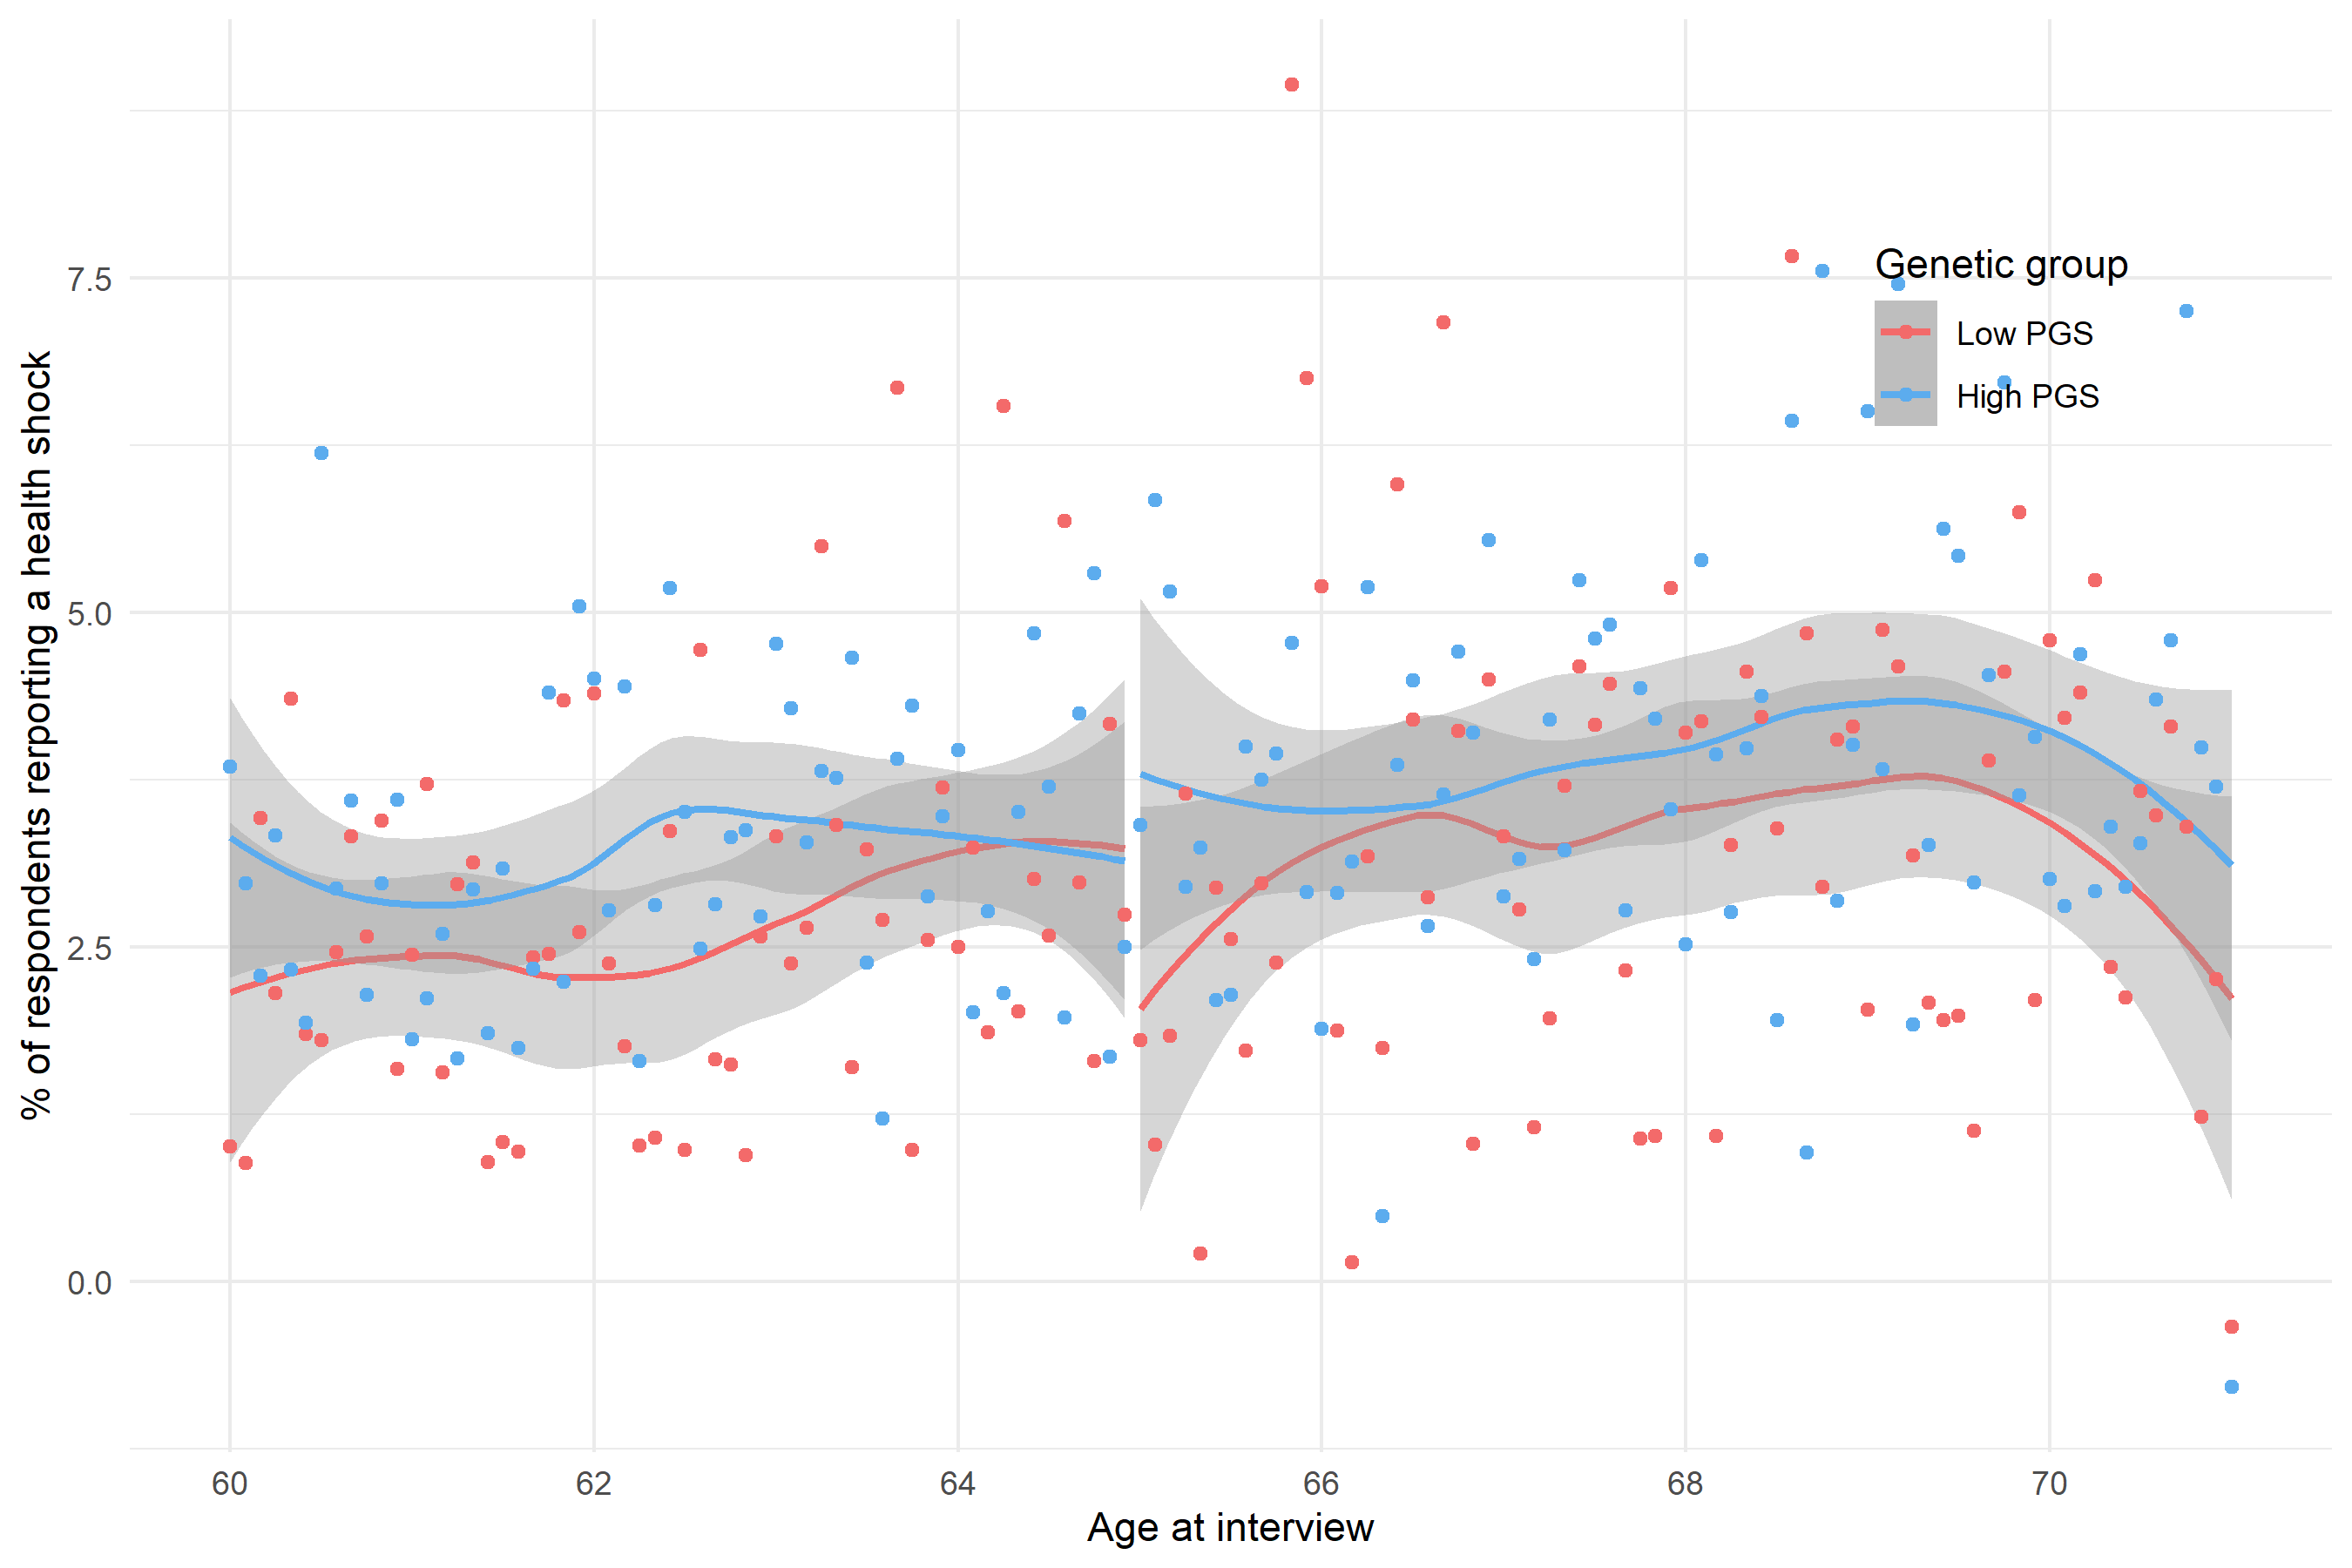
\includegraphics[width=0.9\textheight]{../../3_output/over_time/graph_6070cvrdd_agebypgs.png}
\label{fig:cv_prob_rdd}
\end{figure}


%\begin{figure}[hbtp]
%%\caption{Percentage of Reported Health Shocks by Age}
%\centering
%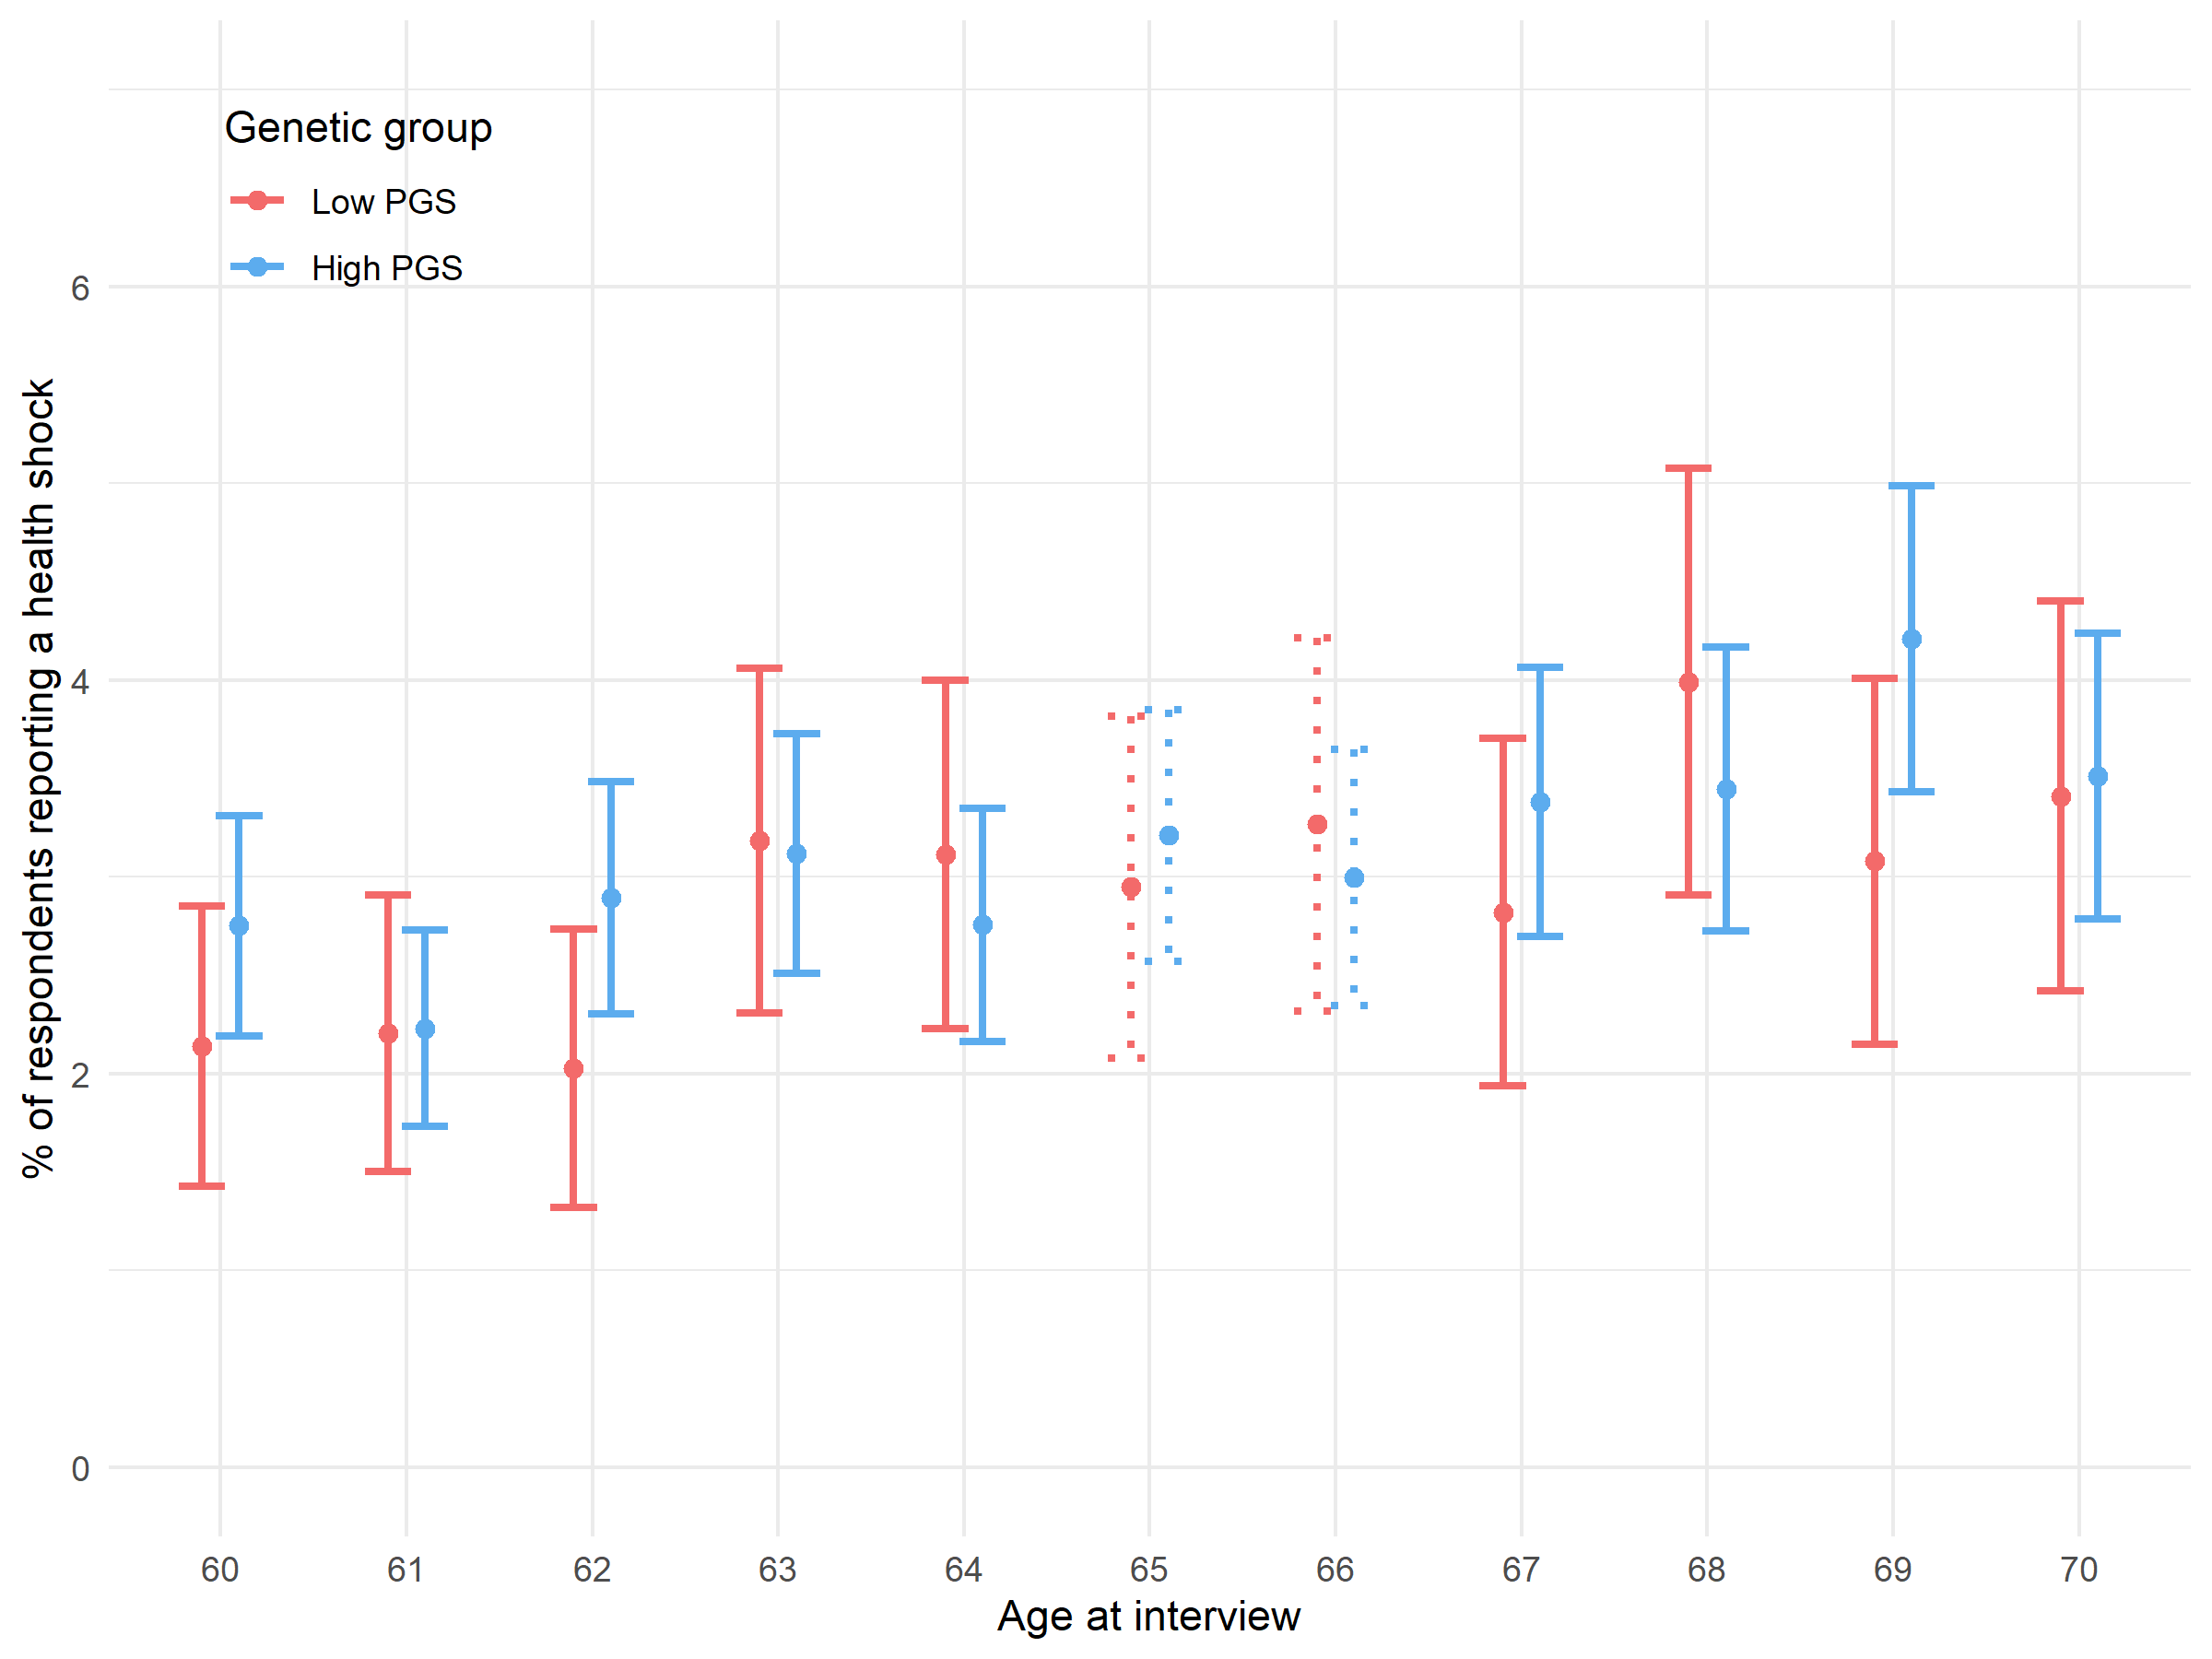
\includegraphics[height=0.75\textheight]{../../3_output/cv_prob/main_6070plot_pgs.png}
%\label{fig:cv_prob}
%\end{figure}
%
%\begin{figure}[!tbp]
%	\begin{center}
%		\caption{Percentage of Reported Health Shocks by Age \label{fig:cv_prob}}
%		\subfigure[\textsf{Average by year}]{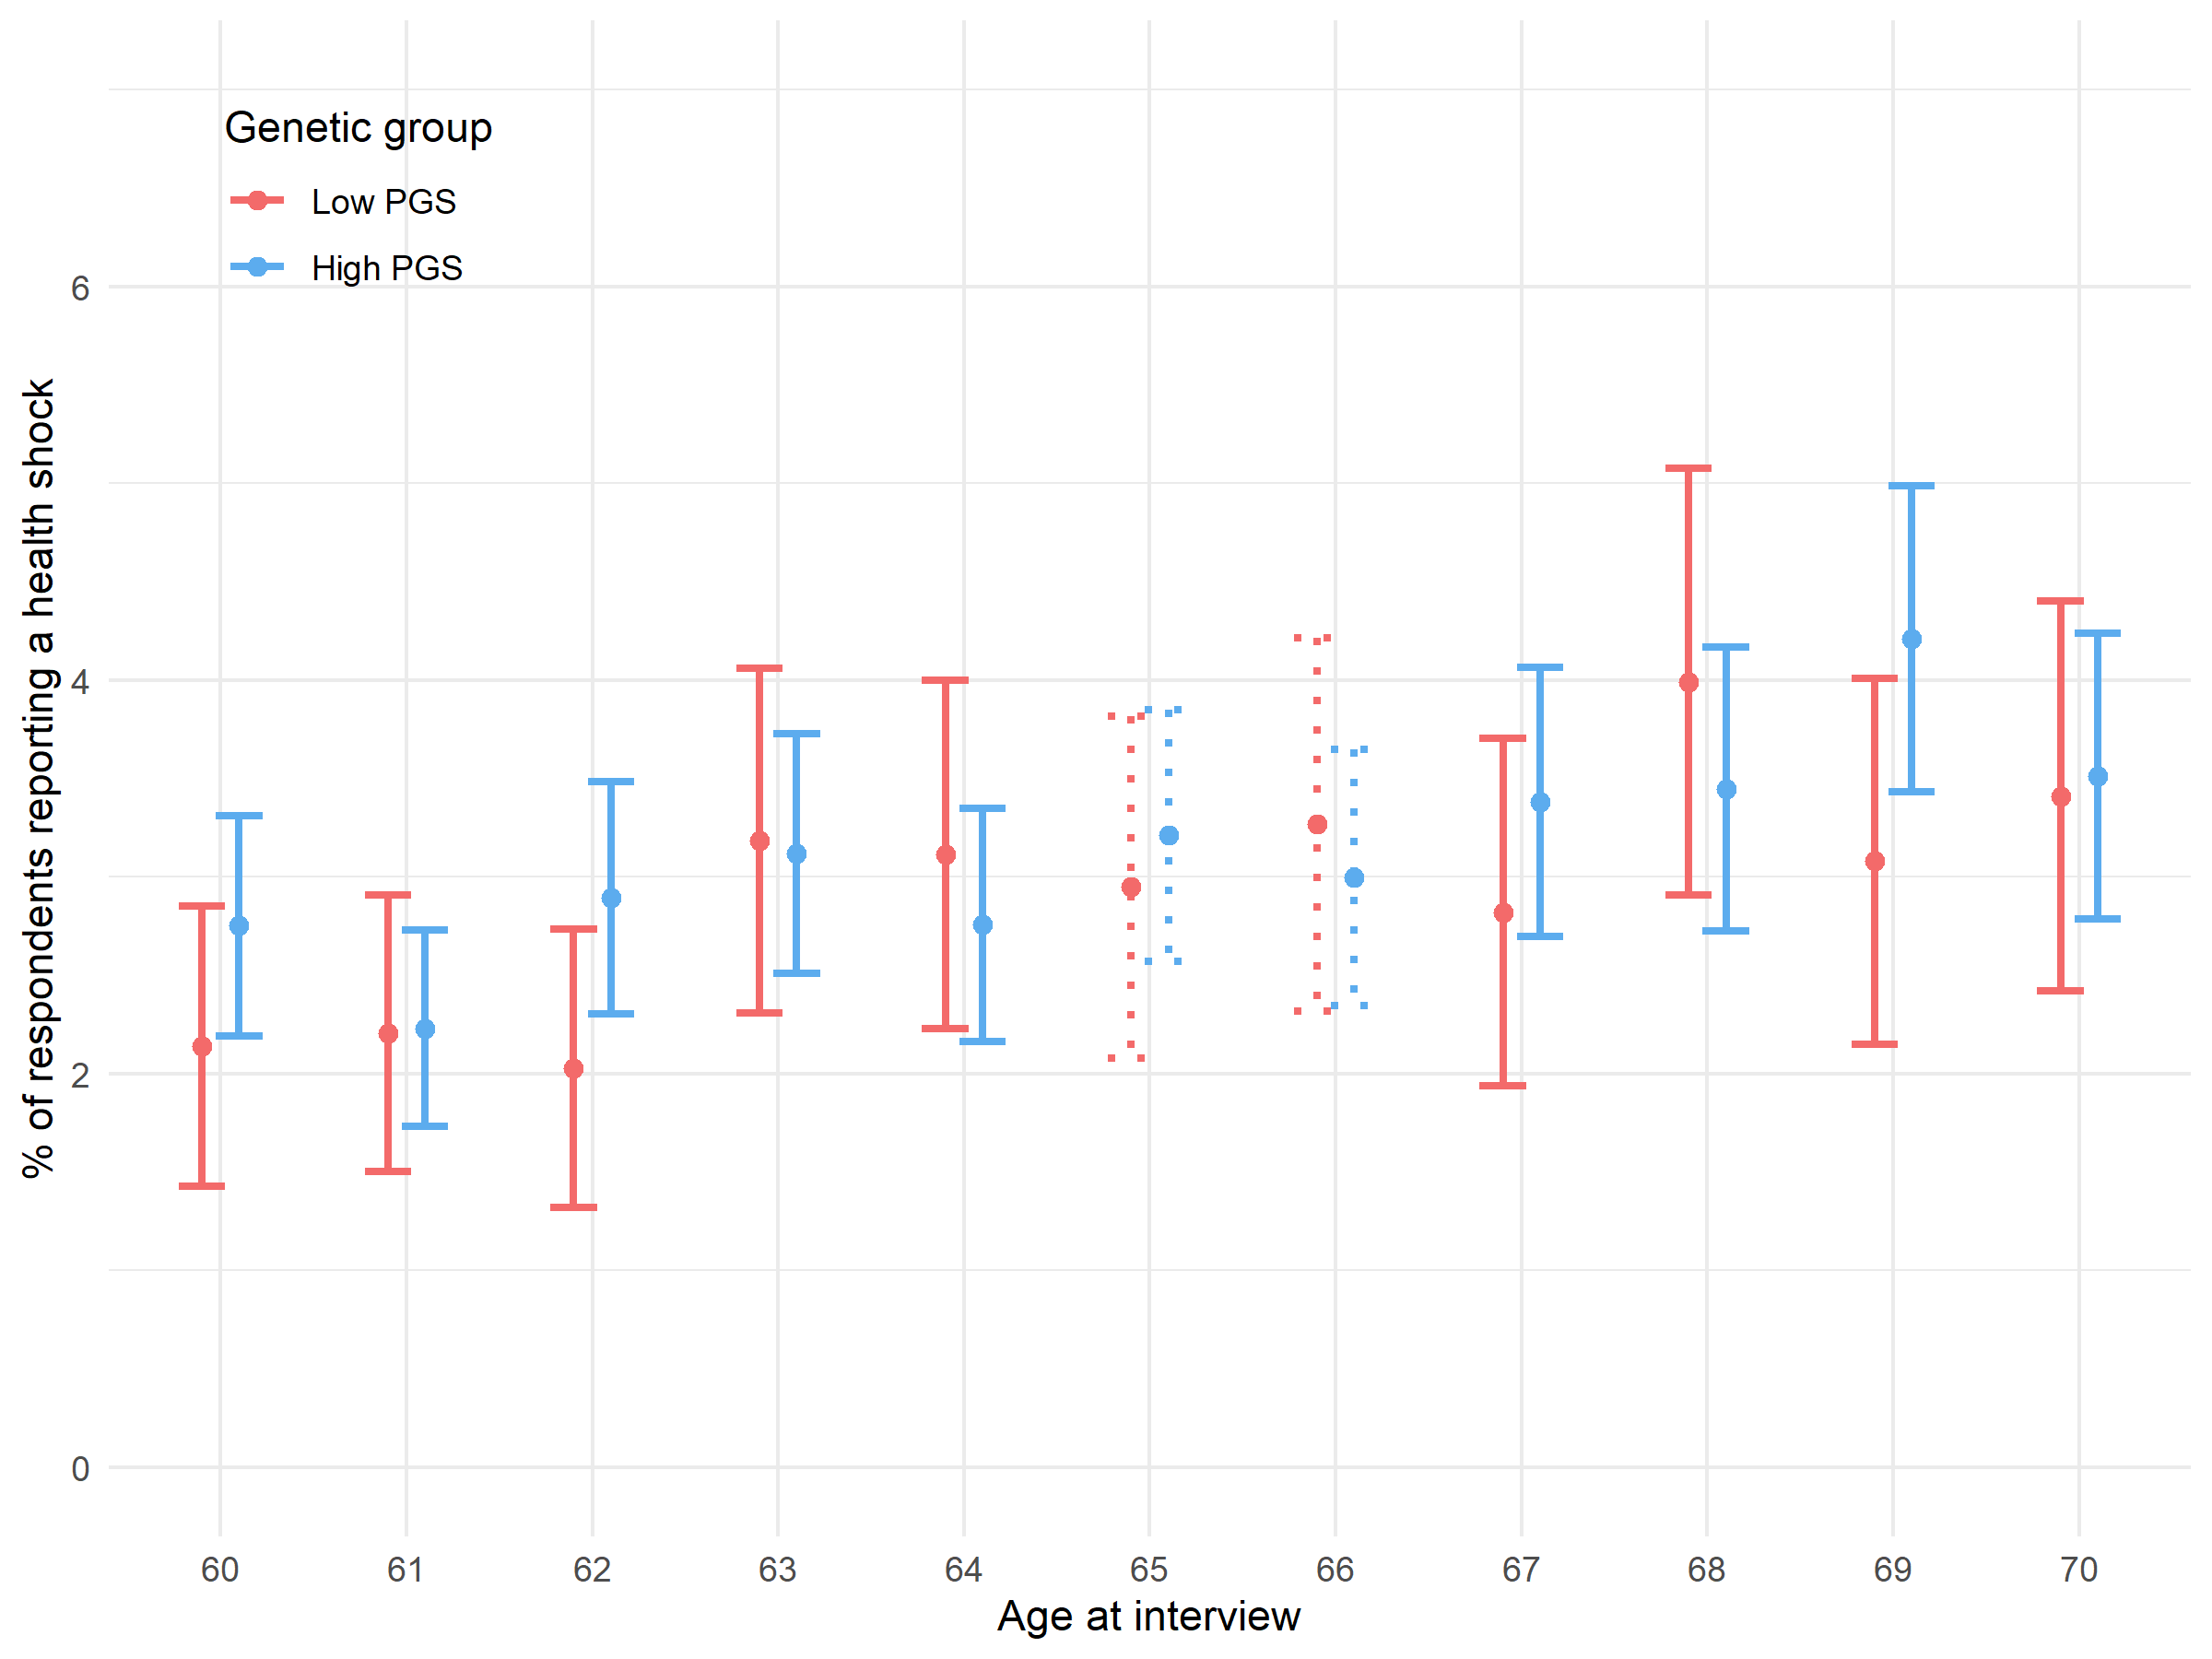
\includegraphics[width=0.4\textheight]{../../3_output/cv_prob/main_6070plot_pgs.png} }
%		\hfill
%		\subfigure[\textsf{RDD}]{\includegraphics[width=0.4\textheight]{../../3_output/cv_prob/RD_age65_CVshock.png} }
%		%\floatfoot{ \vspace{-0.8cm} \\
%		%	\textsf{Low PGS: PGS $\leq$ median PGS. High PGS: PGS $>$ median PGS. \\
%		%		Bars show 95\% confidence intervals. Dotted bars indicate that it was unknown if reported shocks occurred before or after age 65. \\
%		%		Data used: HRS waves 1-12, restricted to observations with age between 60 and 70 years and non-missing smoking status.}}
%	\end{center}
%\end{figure}
%
\end{frame}


%--------------------------------------------------------------%
\begin{frame}
\frametitle{Summary statistics}\label{frame:sumstats}
\begin{table}[ht]
	\caption{Descriptive Statistics for Full Analytic Sample and Stratified by Genetic Group}
	\small\resizebox{1.0\textheight}{!}{
		% latex table generated in R 4.0.2 by xtable 1.8-4 package
% 
\begin{tabular}{llll}
  \toprule
\textbf{ } & \textbf{ All } & \textbf{ Low PGS } & \textbf{ High PGS } \\ 
  \midrule
 & Mean (SD) & Mean (SD) & Mean (SD) \\ 
   \midrule
Age (baseline) & 61.17 (1.93) & 61.18 (1.96) & 61.16 (1.92) \\ 
  Smoking PGS & 0.11 (0.99) & -0.96 (0.51) & 0.64 (0.71) \\ 
  No. waves present & 4.44 (1.38) & 4.46 (1.37) & 4.43 (1.39) \\ 
   & \% & \% & \% \\ 
  Female & 50.42 & 46.97 & 52.14 \\ 
  Smoking (baseline) & 29.55 & 27.06 & 30.79 \\ 
  Persistently uninsured & 5.85 & 5.39 & 6.08 \\ 
  CV health shock & 12.44 & 11.82 & 12.74 \\ 
   \midrule
No. of individuals & 5813 & 1929 & 3884 \\ 
  No. Person-year observations & 25800 & 8602 & 17198 \\ 
   \bottomrule
\end{tabular}

	}
\end{table}

\hyperlink{frame:sumstats2}{\beamergotobutton{Sumstats2}}
\hyperlink{frame:uninsured}{\beamergotobutton{Uninsured}}

\end{frame}

%--------------------------------------------------------------%
\begin{frame}
\frametitle{Smoking rates decrease with age}
Share of smokers over different ages, split by PGS

\begin{figure}[hbtp]
\centering
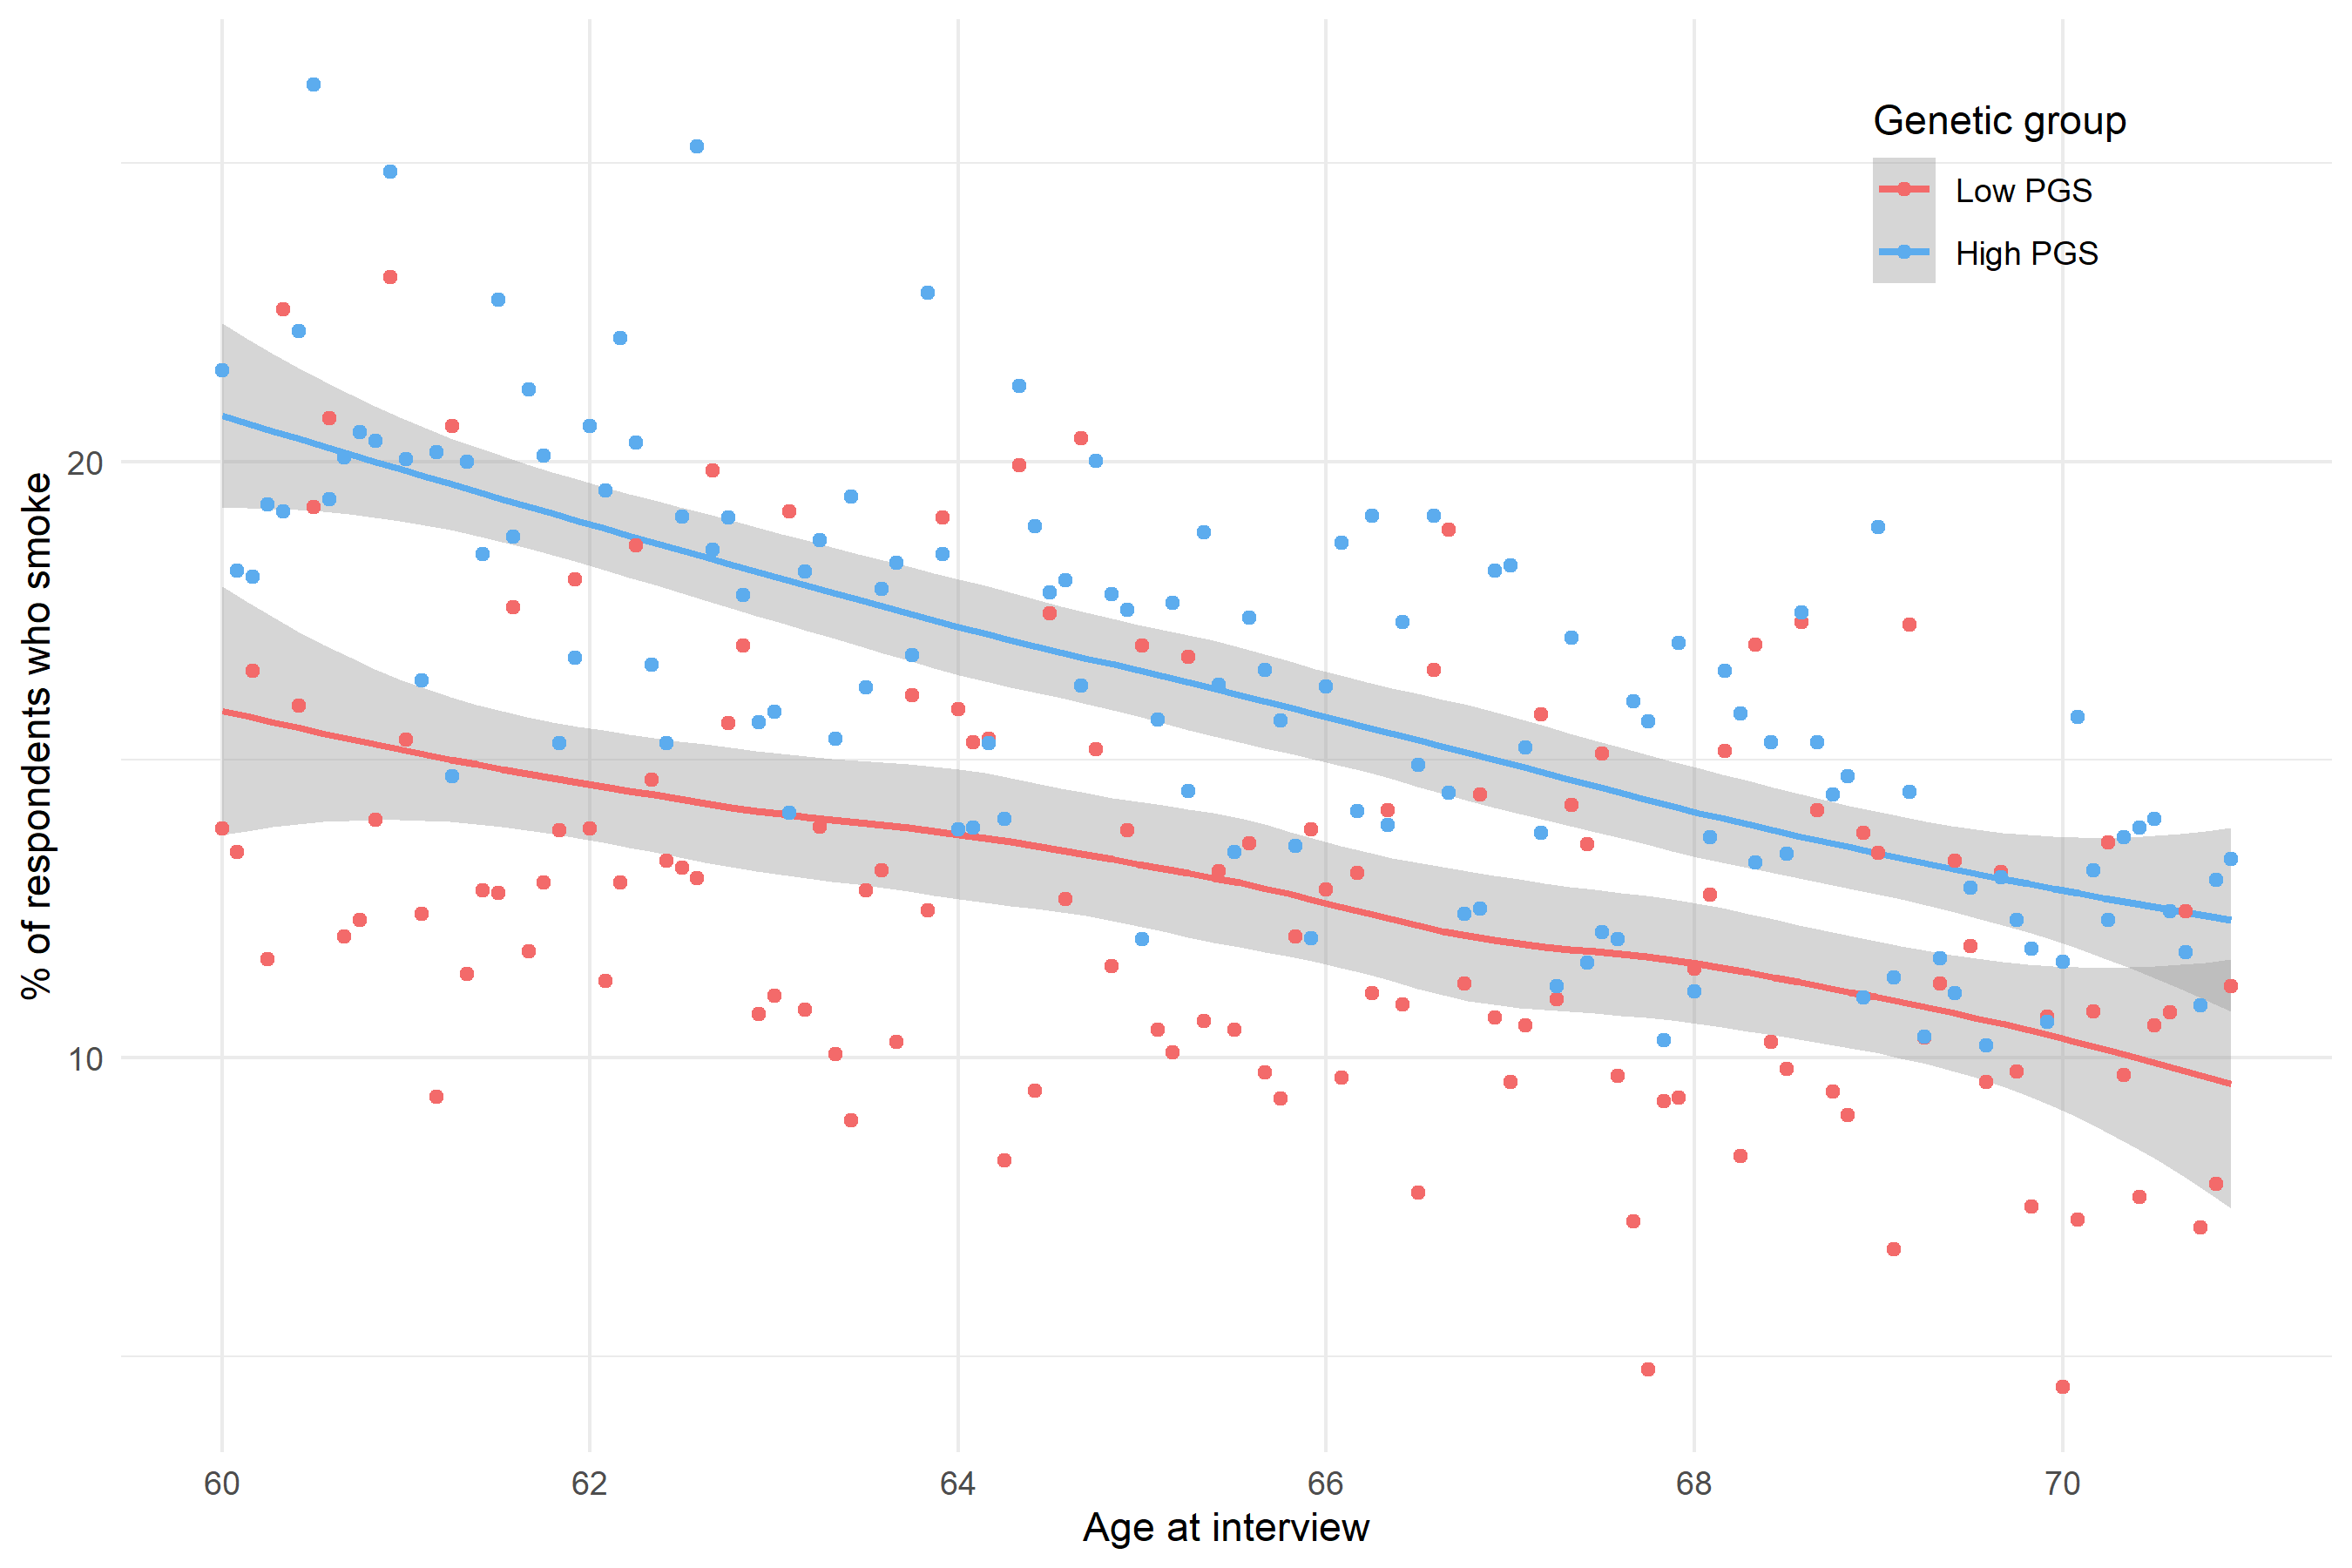
\includegraphics[height=0.8\textheight]{../../3_output/over_time/graph_6070smokenplot_agebypgs.png}
\label{fig:}
\end{figure}

\end{frame}

%--------------------------------------------------------------%
\subsection{Regression}
%--------------------------------------------------------------%
\begin{frame}\frametitle{Regression analysis}
\vspace{-5ex}
\begin{footnotesize}

\begin{align*} \label{eq:OLS}
Y_{it}& \thinspace  = \thinspace
				\beta \thinspace shock_{it} + \gamma \thinspace post65_{it} \\
				&+\lambda_1 \thinspace  (shock_{it} \times post65_{it}) \nonumber \\
				&+ \lambda_2 \thinspace (shock_{it} \times uninsured_i) \nonumber \\
				&+\lambda_3  \thinspace (post65_{it} \times uninsured_i) \nonumber \\
				&+ \lambda_4 \thinspace (shock_{it} \times g_i) \nonumber \\
				&+\lambda_5 \thinspace (post65_{it} \times g_i) \nonumber \\
				&+ \delta_1 \thinspace (shock_{it} \times post65_{it} \times uninsured_i) \nonumber \\
				&+ \delta_2 \thinspace (shock_{it} \times uninsured_i \times g_i) \nonumber \\
				&+ \delta_3 \thinspace (shock_{it} \times post65_{it} \times g_i) \nonumber \\
				&+ \delta_4 \thinspace (post65_{it} \times uninsured_i \times g_i) \nonumber\\
				&+ \zeta \thinspace (shock_{it} \times post65_{it} \times uninsured_i \times g_i) \nonumber \\
				&+ \sum_{a=1}^3 \phi_a \thinspace age_{it}^{a} + \eta_i + \tau_t + \varepsilon_{it} \nonumber
\end{align*}

Current smoking status ($Y$) regressed on the full set of interactions between the indicators for the health shock ($shock$), being uninsured pre-65 ($uninsured$), Medicare eligibility ($post65$), and high polygenic risk for smoking ($g$).

Controlling for age + individual and time F.E.
\end{footnotesize}

\end{frame}

%--------------------------------------------------------------%
\begin{frame}
\frametitle{Effect of the shock on the outcomes} \label{frame:shockmath}
The derivative of the outcome with respect to shock is:
%\hyperlink{fig:maincoeffplot}{\beamergotobutton{back}}

\begin{footnotesize}
\begin{align}
\begin{aligned}
	\frac{\partial Y_{it}}{\partial shock_{it}}&=\beta+\lambda_1post65_{it}+\lambda_2uninsured_{i}+\lambda_4g_i+\delta_1(post65 \times uninsured_i)+\delta_2(uninsured_i \times g_i) \\
	&+\delta_3(post65_{it} \times g_i)+\xi(post65_{it} \times uninsured_i \times g_i)
\end{aligned}
\end{align}

Looking at the effect for the four different types (before-after 65, high-low g):
\begin{align}
\phantom{E\left[ \frac{\partial Y_{it}}{\partial shock_{it}}| post65_{it}=1, g_i=1,uninsured_i=1\right]}
&\begin{aligned}
\mathllap{E\left[ \frac{\partial Y_{it}}{\partial shock_{it}}| post65_{it}=0, g_i=0,uninsured_i=1\right]} &=\beta+\lambda_2
\end{aligned}\\
&\begin{aligned}
\mathllap{E\left[ \frac{\partial Y_{it}}{\partial shock_{it}}| post65_{it}=1, g_i=0,uninsured_i=1\right]} &=\beta+\lambda_1+\lambda_2+\delta_1
\end{aligned}\\
&\begin{aligned}
\mathllap{E\left[ \frac{\partial Y_{it}}{\partial shock_{it}}| post65_{it}=0, g_i=1,uninsured_i=1\right]} &=\beta+\lambda_2+\lambda_4+\delta_2
\end{aligned}\\
&\begin{aligned}
\mathllap{E\left[ \frac{\partial Y_{it}}{\partial shock_{it}}| post65_{it}=1, g_i=1,,uninsured_i=1\right]} &=\beta+\lambda_1+\lambda_2+\lambda_4+\delta_1+\delta_2+\delta_3+\xi
\end{aligned}
\end{align}

Calculating the first two differences as above:

\begin{align}
(10)-(9)&=\lambda_1+\delta_1\\
(12)-(11)&=\lambda_1+\delta_1+\delta_3+\xi
\end{align}

And the diff-in-diff (G$\times$E):
\begin{align}
(14)-(13)&=\delta_3+\xi
\end{align}
\end{footnotesize}

\end{frame}

%--------------------------------------------------------------%
\begin{frame}
\frametitle{Regression results}
Controlling for individual and time F.E. + age:

\begin{figure}[hbtp]
\centering
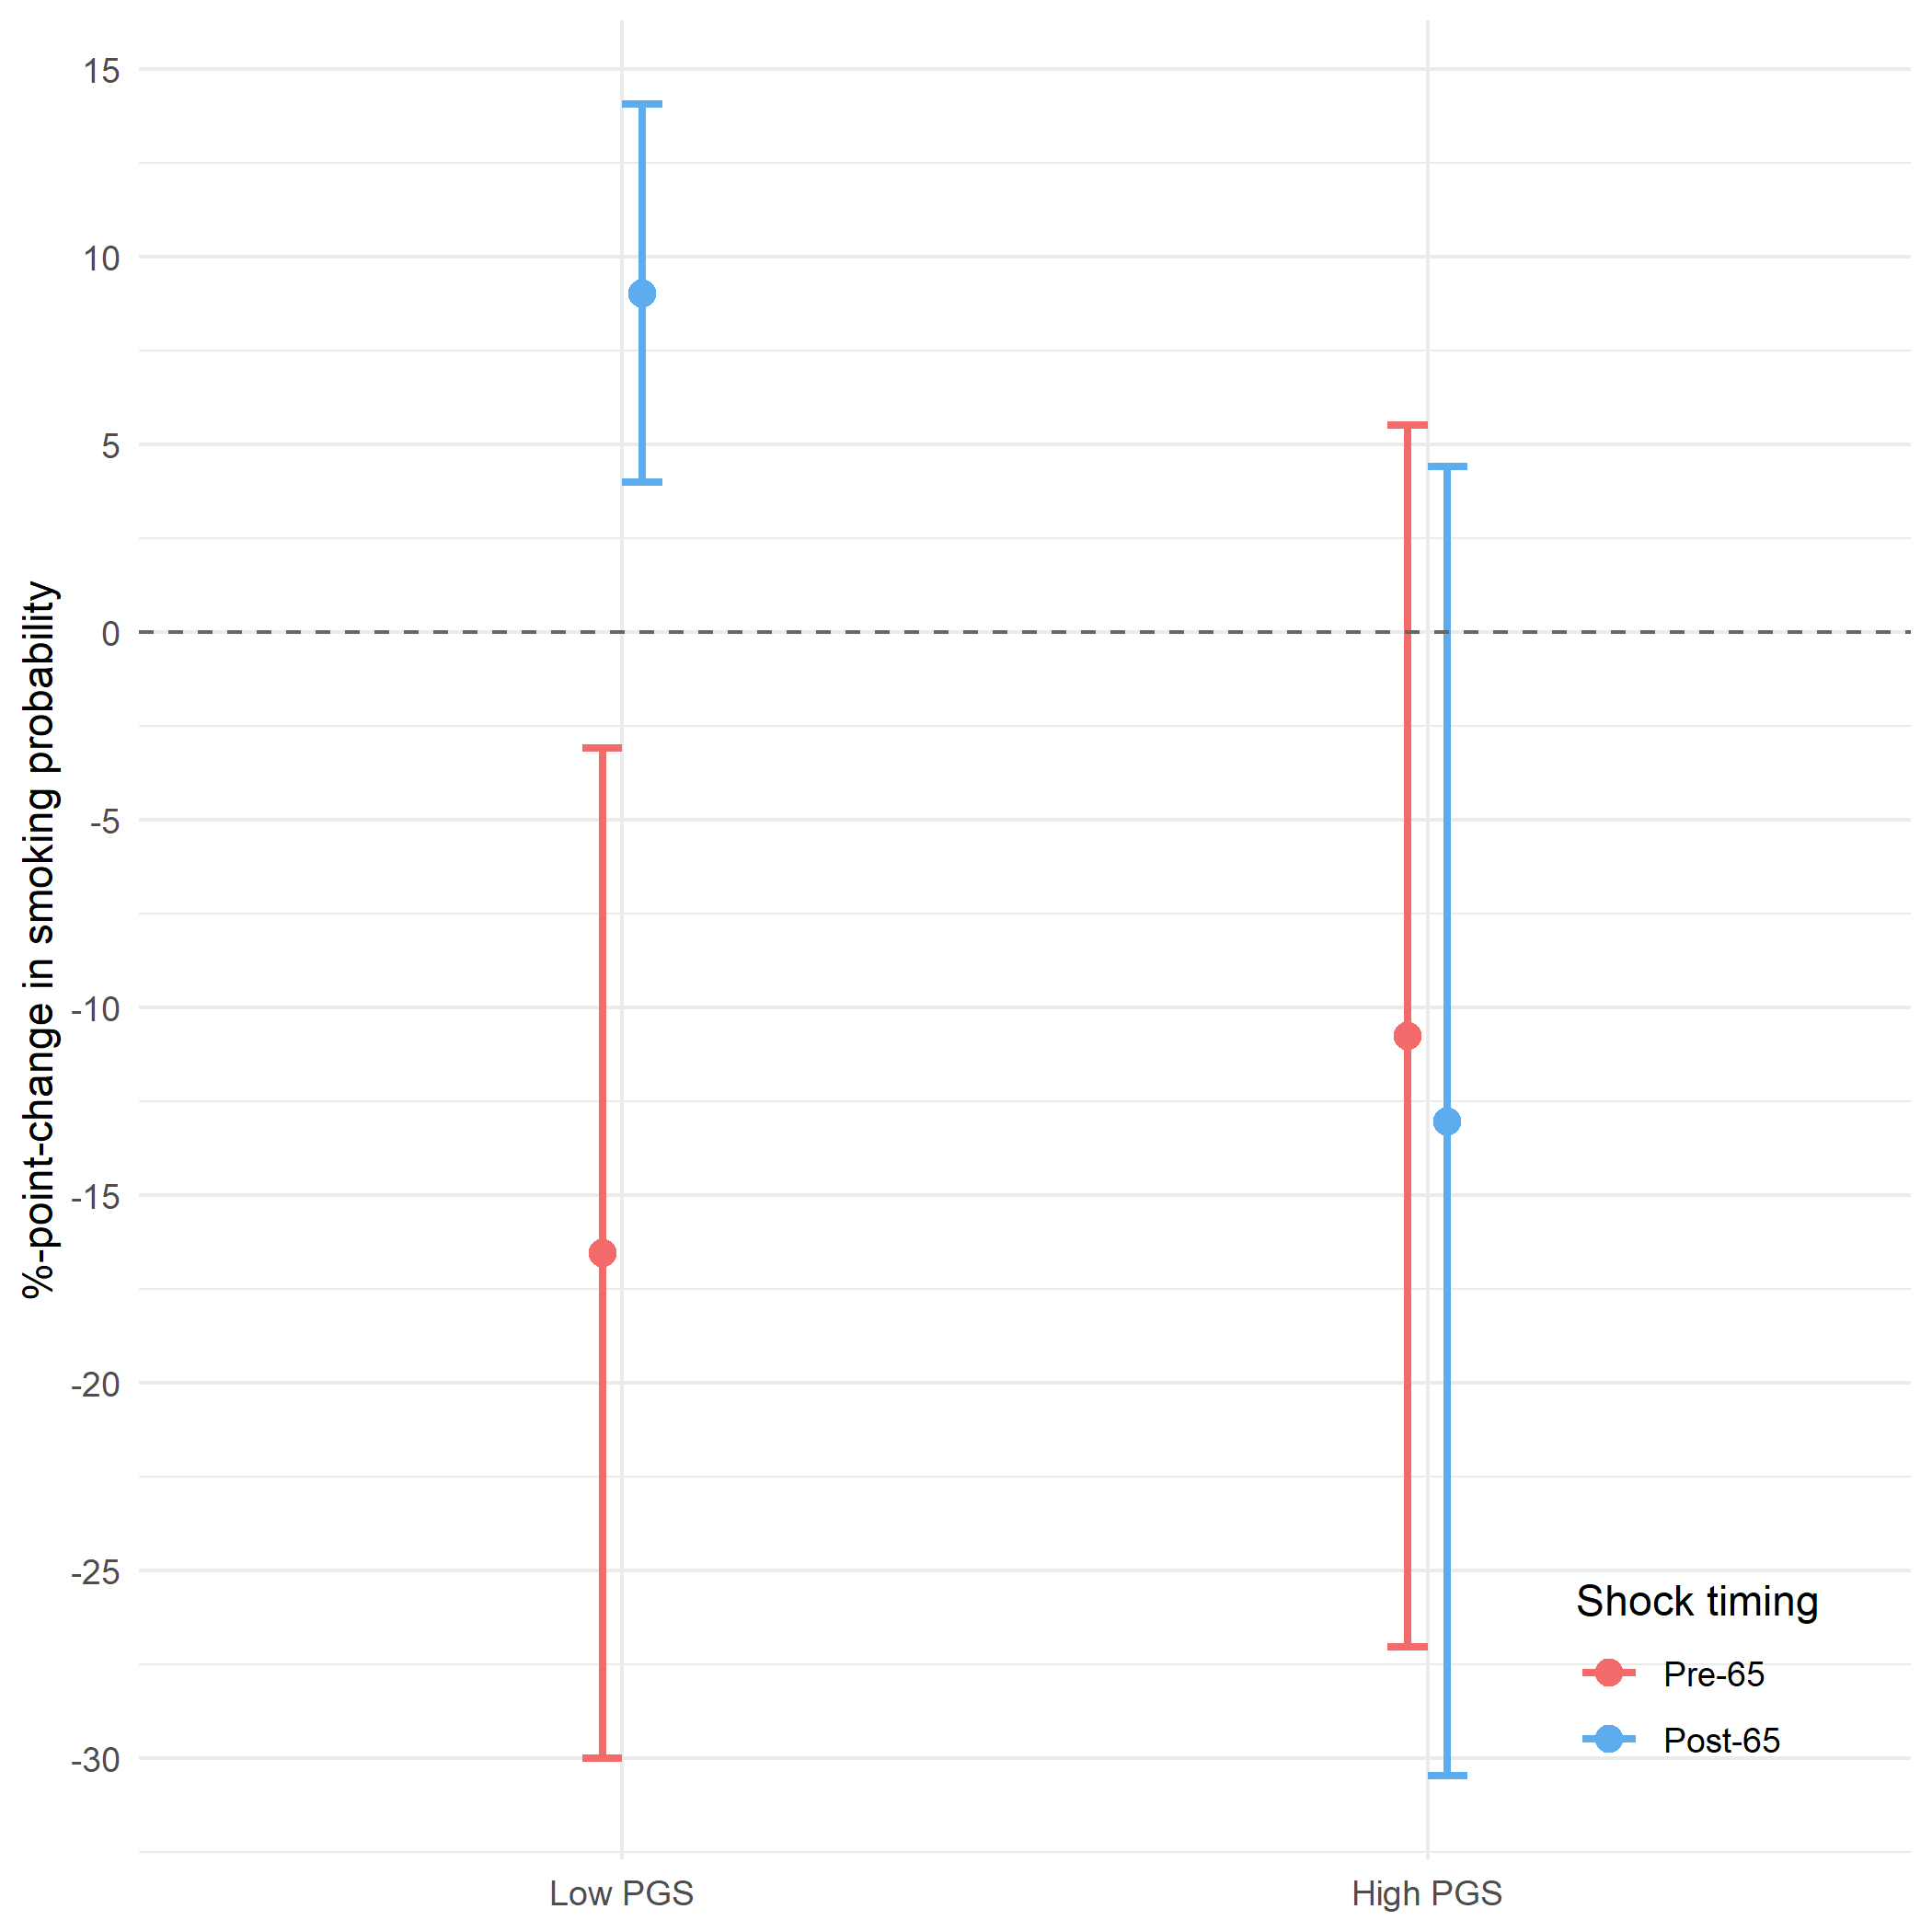
\includegraphics[height=0.8\textheight]{../../3_output/shock_effects/main_6070_100_cv.png}
\label{fig:maincoeffplot}
\end{figure}
\hyperlink{frame:fullreg}{\beamergotobutton{all coefficients}}
%\hyperlink{frame:robustness}{\beamergotobutton{robustness}}

\end{frame}

%--------------------------------------------------------------%
\begin{frame}
\frametitle{Evidence of $G \times E$} \label{frame:regtab}

\begin{table}[ht]
	\caption{Effect of the shock by timing and PGS}
	\small\resizebox{0.9\textheight}{!}{
	% latex table generated in R 4.0.2 by xtable 1.8-4 package
% 
\begin{tabular}{lll}
  \toprule
  \multicolumn{3}{c}{ \textbf{Effect of health shock on smoking probability}} \\
 \midrule
 & Low PGS & High PGS \\ 
   \midrule
Pre 65 & -0.165** & -0.108 \\ 
   & (0.069) & (0.083) \\ 
  Post 65 & 0.09*** & -0.13 \\ 
   & (0.026) & (0.089) \\ 
   \toprule \multicolumn{3}{c}{ \textbf{Effect of health insurance on effect of health shock}} \\
 \midrule
 & Low PGS & High PGS \\ 
   \midrule
Post 65 - Pre 65 & 0.256*** & -0.023 \\ 
   & (0.079) & (0.121) \\ 
   \toprule \multicolumn{3}{c}{ \textbf{Differential effect of health insurance by genetic group}} \\
 \midrule
 & High PGS  & - low PGS \\ 
   \midrule
Post 65 - Pre 65 & -0.279* &  \\ 
   & (0.144) &  \\ 
   \bottomrule
\end{tabular}

	}

	\vspace{1ex}
	{\raggedright \tiny \textit{Notes:} Summary of the effect of the shock on smoking for those who were uninsured before 65, stratified by timing of the shock (before vs. after 65) and genetic group (high vs. low PGS) \par}

\end{table}

\end{frame}

%--------------------------------------------------------------%
\begin{frame}
\frametitle{Different PGS cutoffs}

\begin{figure}[hbtp]
\centering
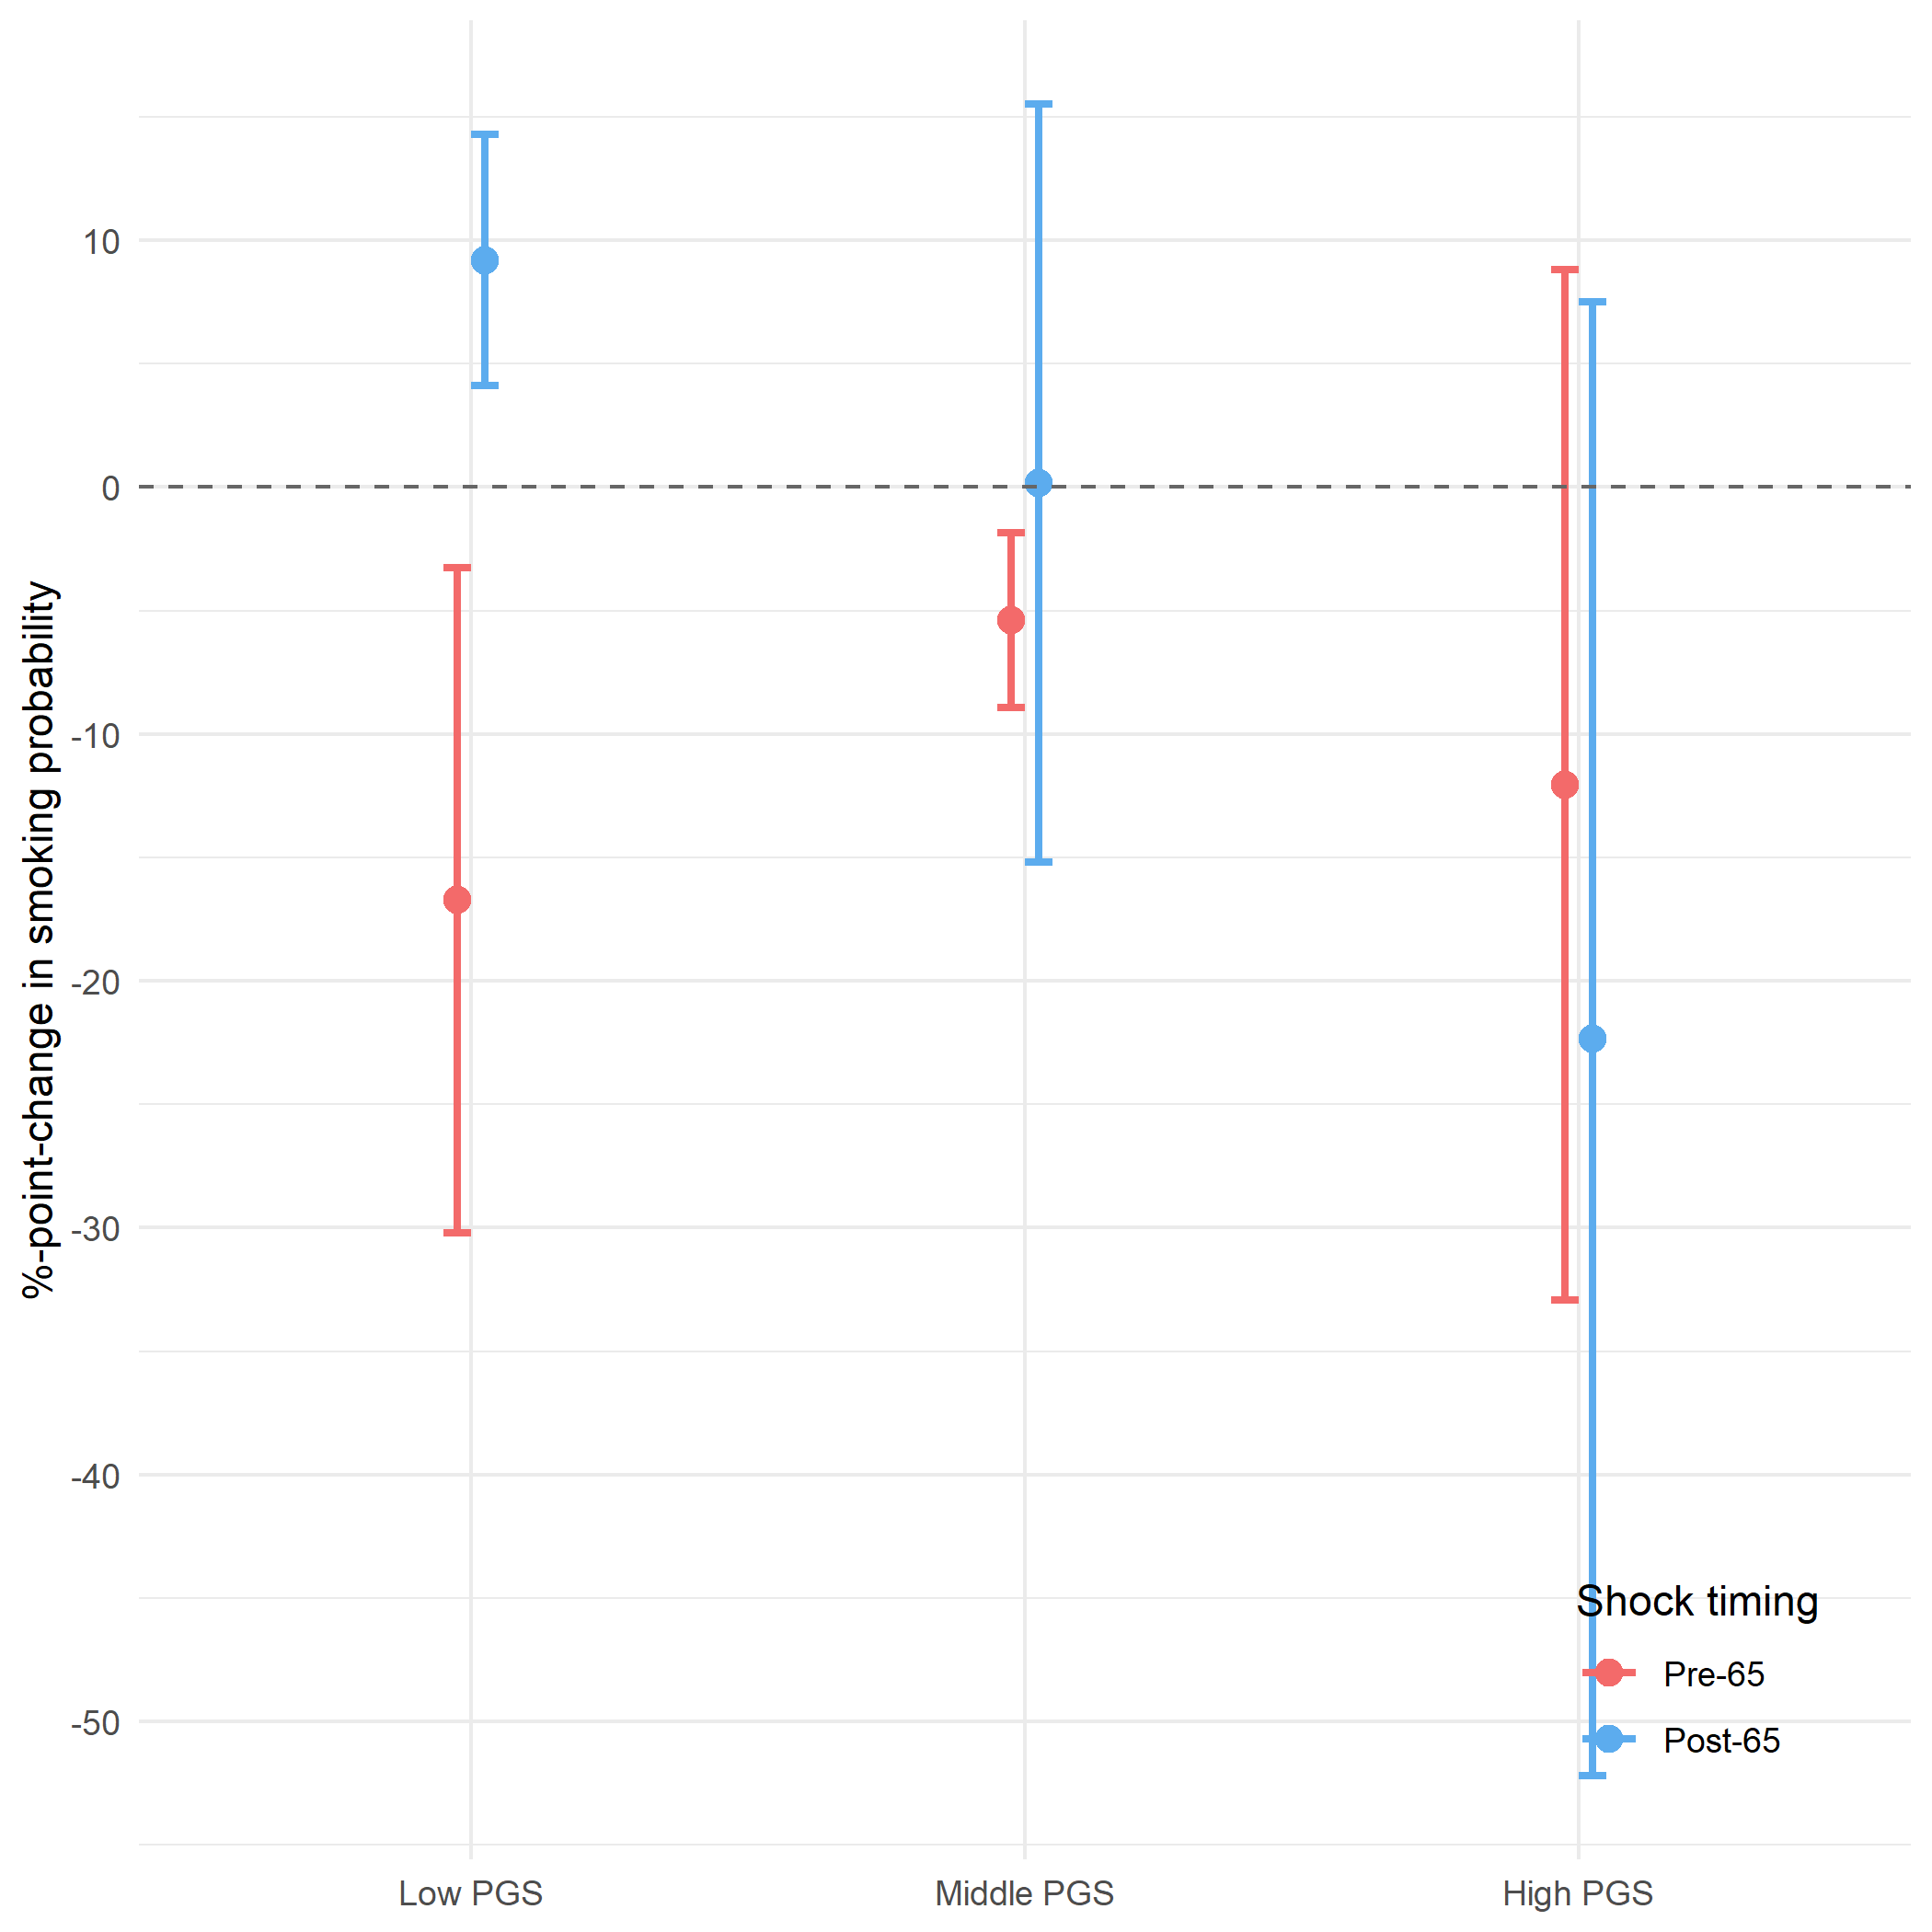
\includegraphics[height=0.8\textheight]{../../3_output/shock_effects/robustness_6070_3pgs_cv.png}
\label{fig:3pgs}
\end{figure}

\end{frame}

%--------------------------------------------------------------%
\section{Sanity Checks}
\subsection{Confounders}
%--------------------------------------------------------------%
\begin{frame}
\frametitle{Potential interpretation problems}
\label{frame:interpret}
What else can drive this relation?
\begin{itemize}
	\item Something that jumps at 65 (besides medicare)
	\begin{itemize}
		\item Retirement and income: no sharp change at age 65 \cite{Card2008,Card2009medicare}
	\end{itemize}
\end{itemize}

\vspace{4ex}

\hspace*{-6ex}
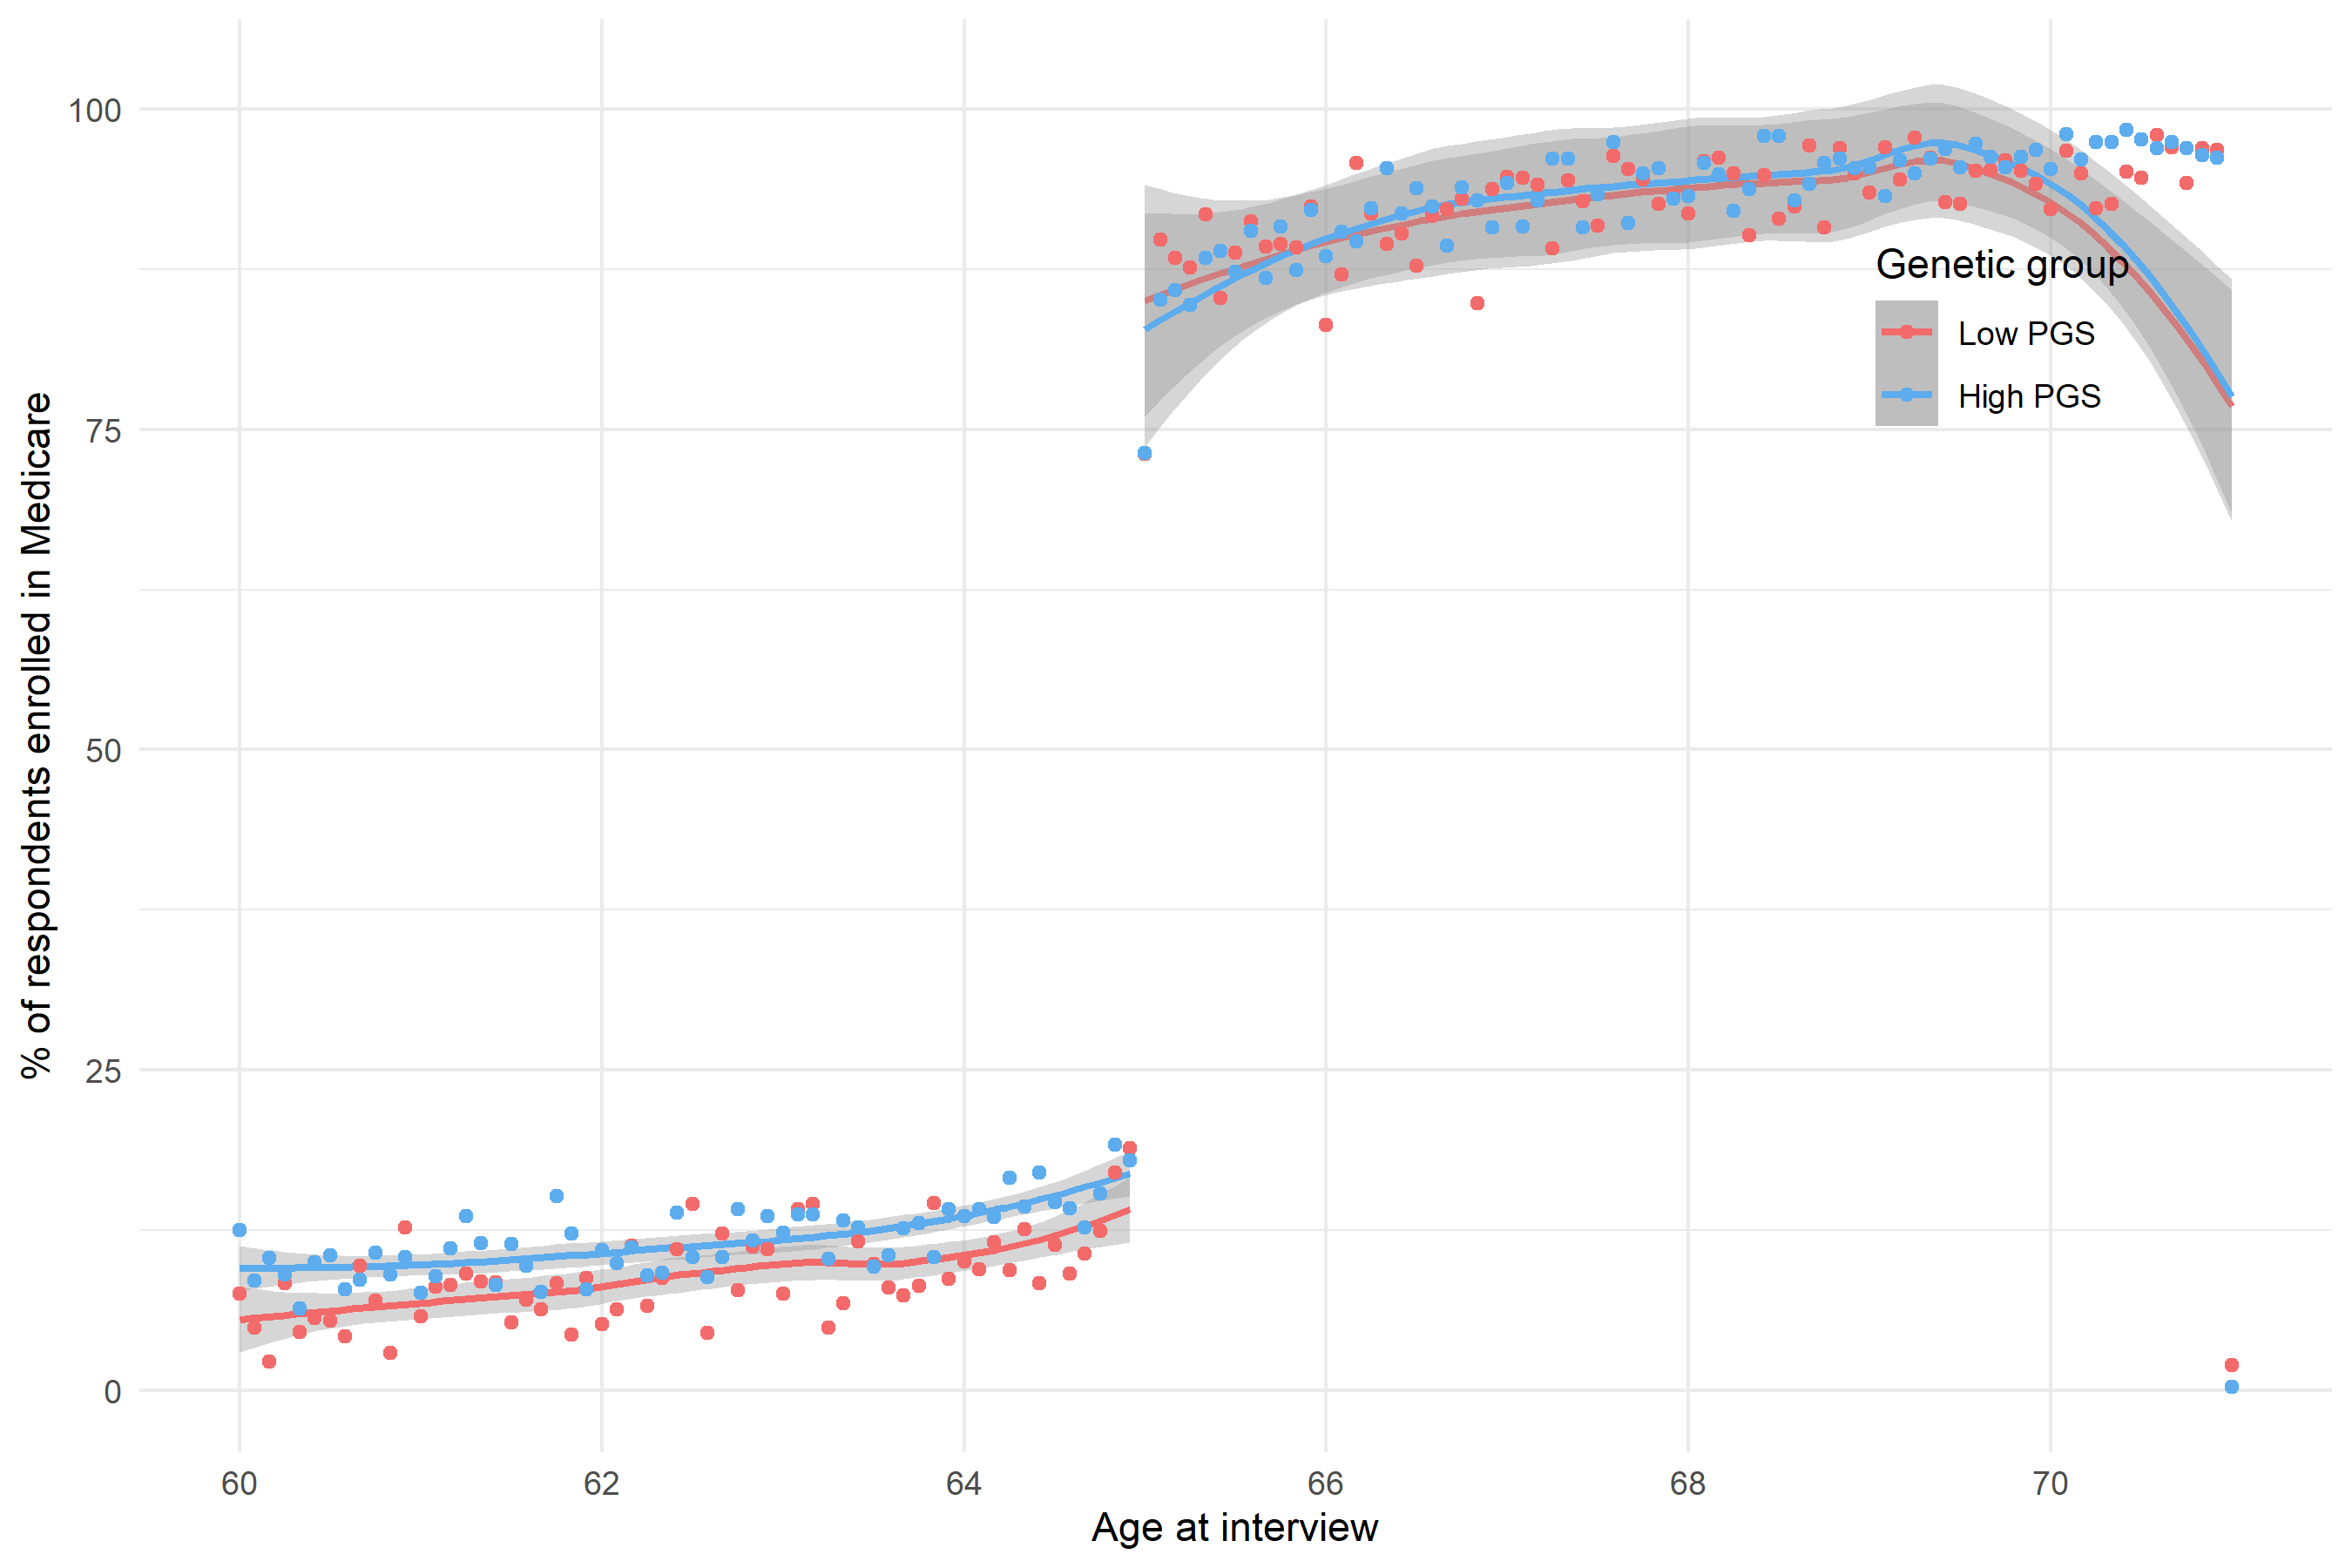
\includegraphics[width=.36\textwidth]{../../3_output/over_time/graph_6070govmrrdd_agebypgs.png}%
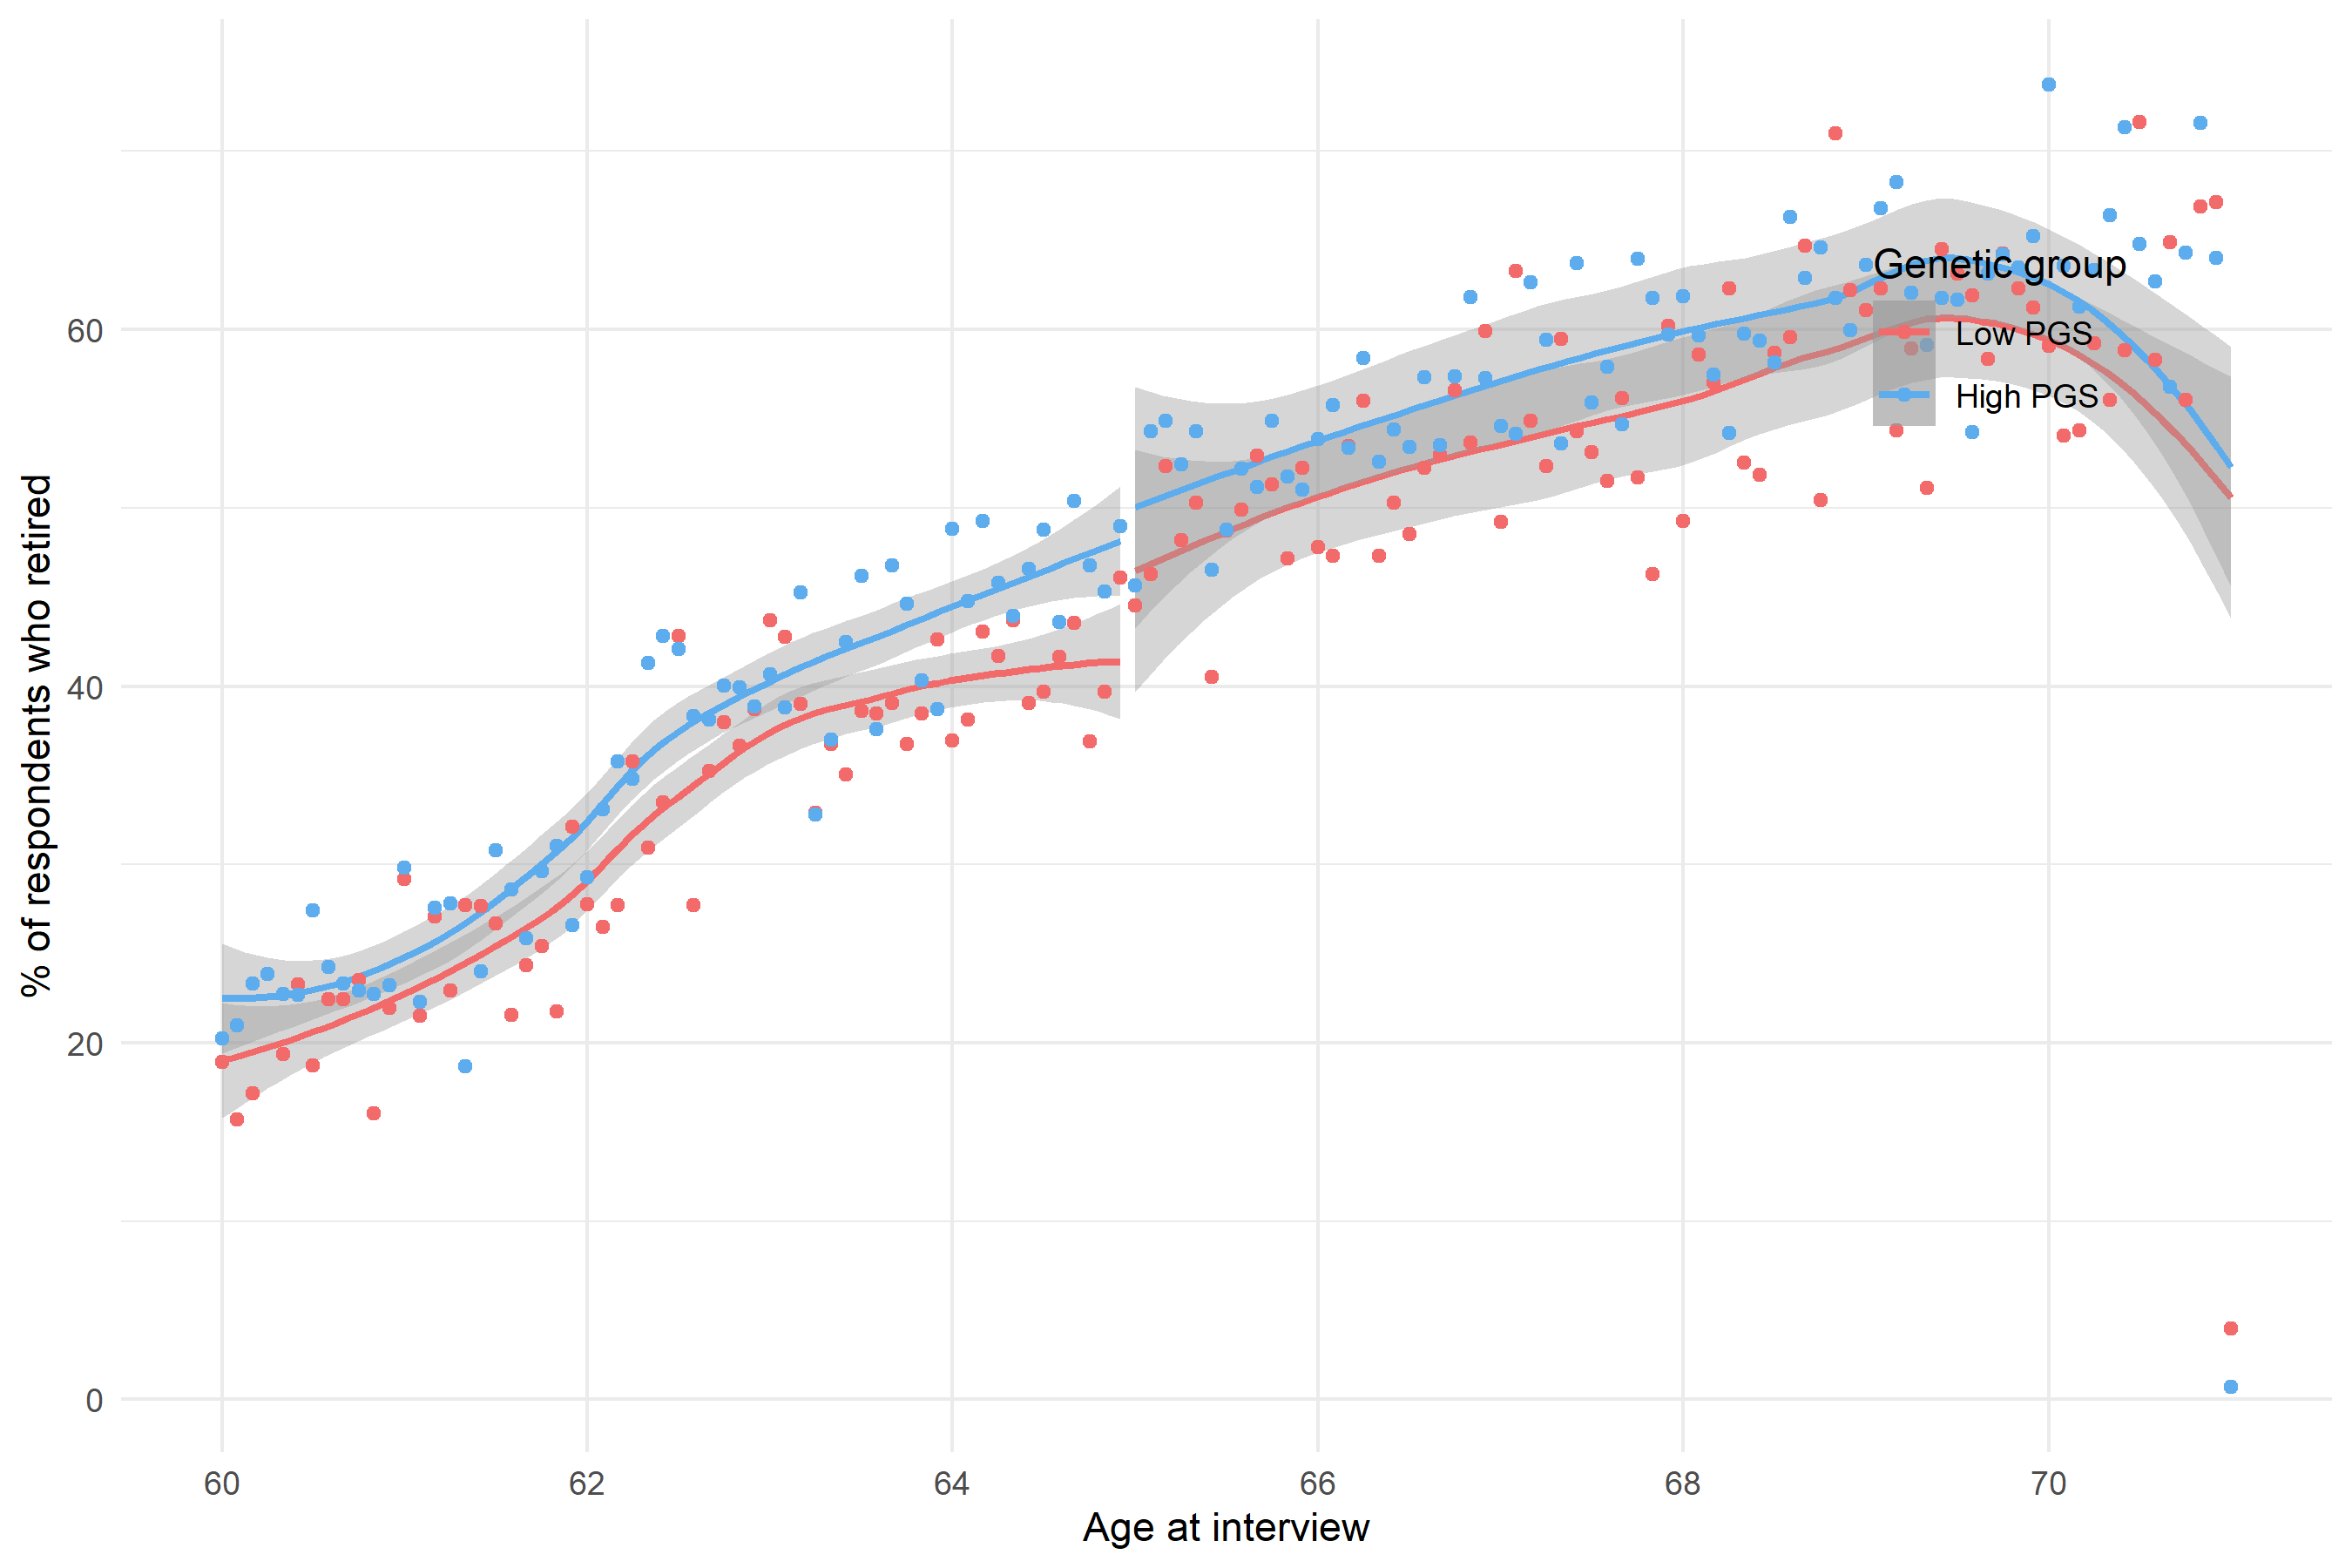
\includegraphics[width=.36\textwidth]{../../3_output/over_time/graph_6070retiredrdd_agebypgs.png}%
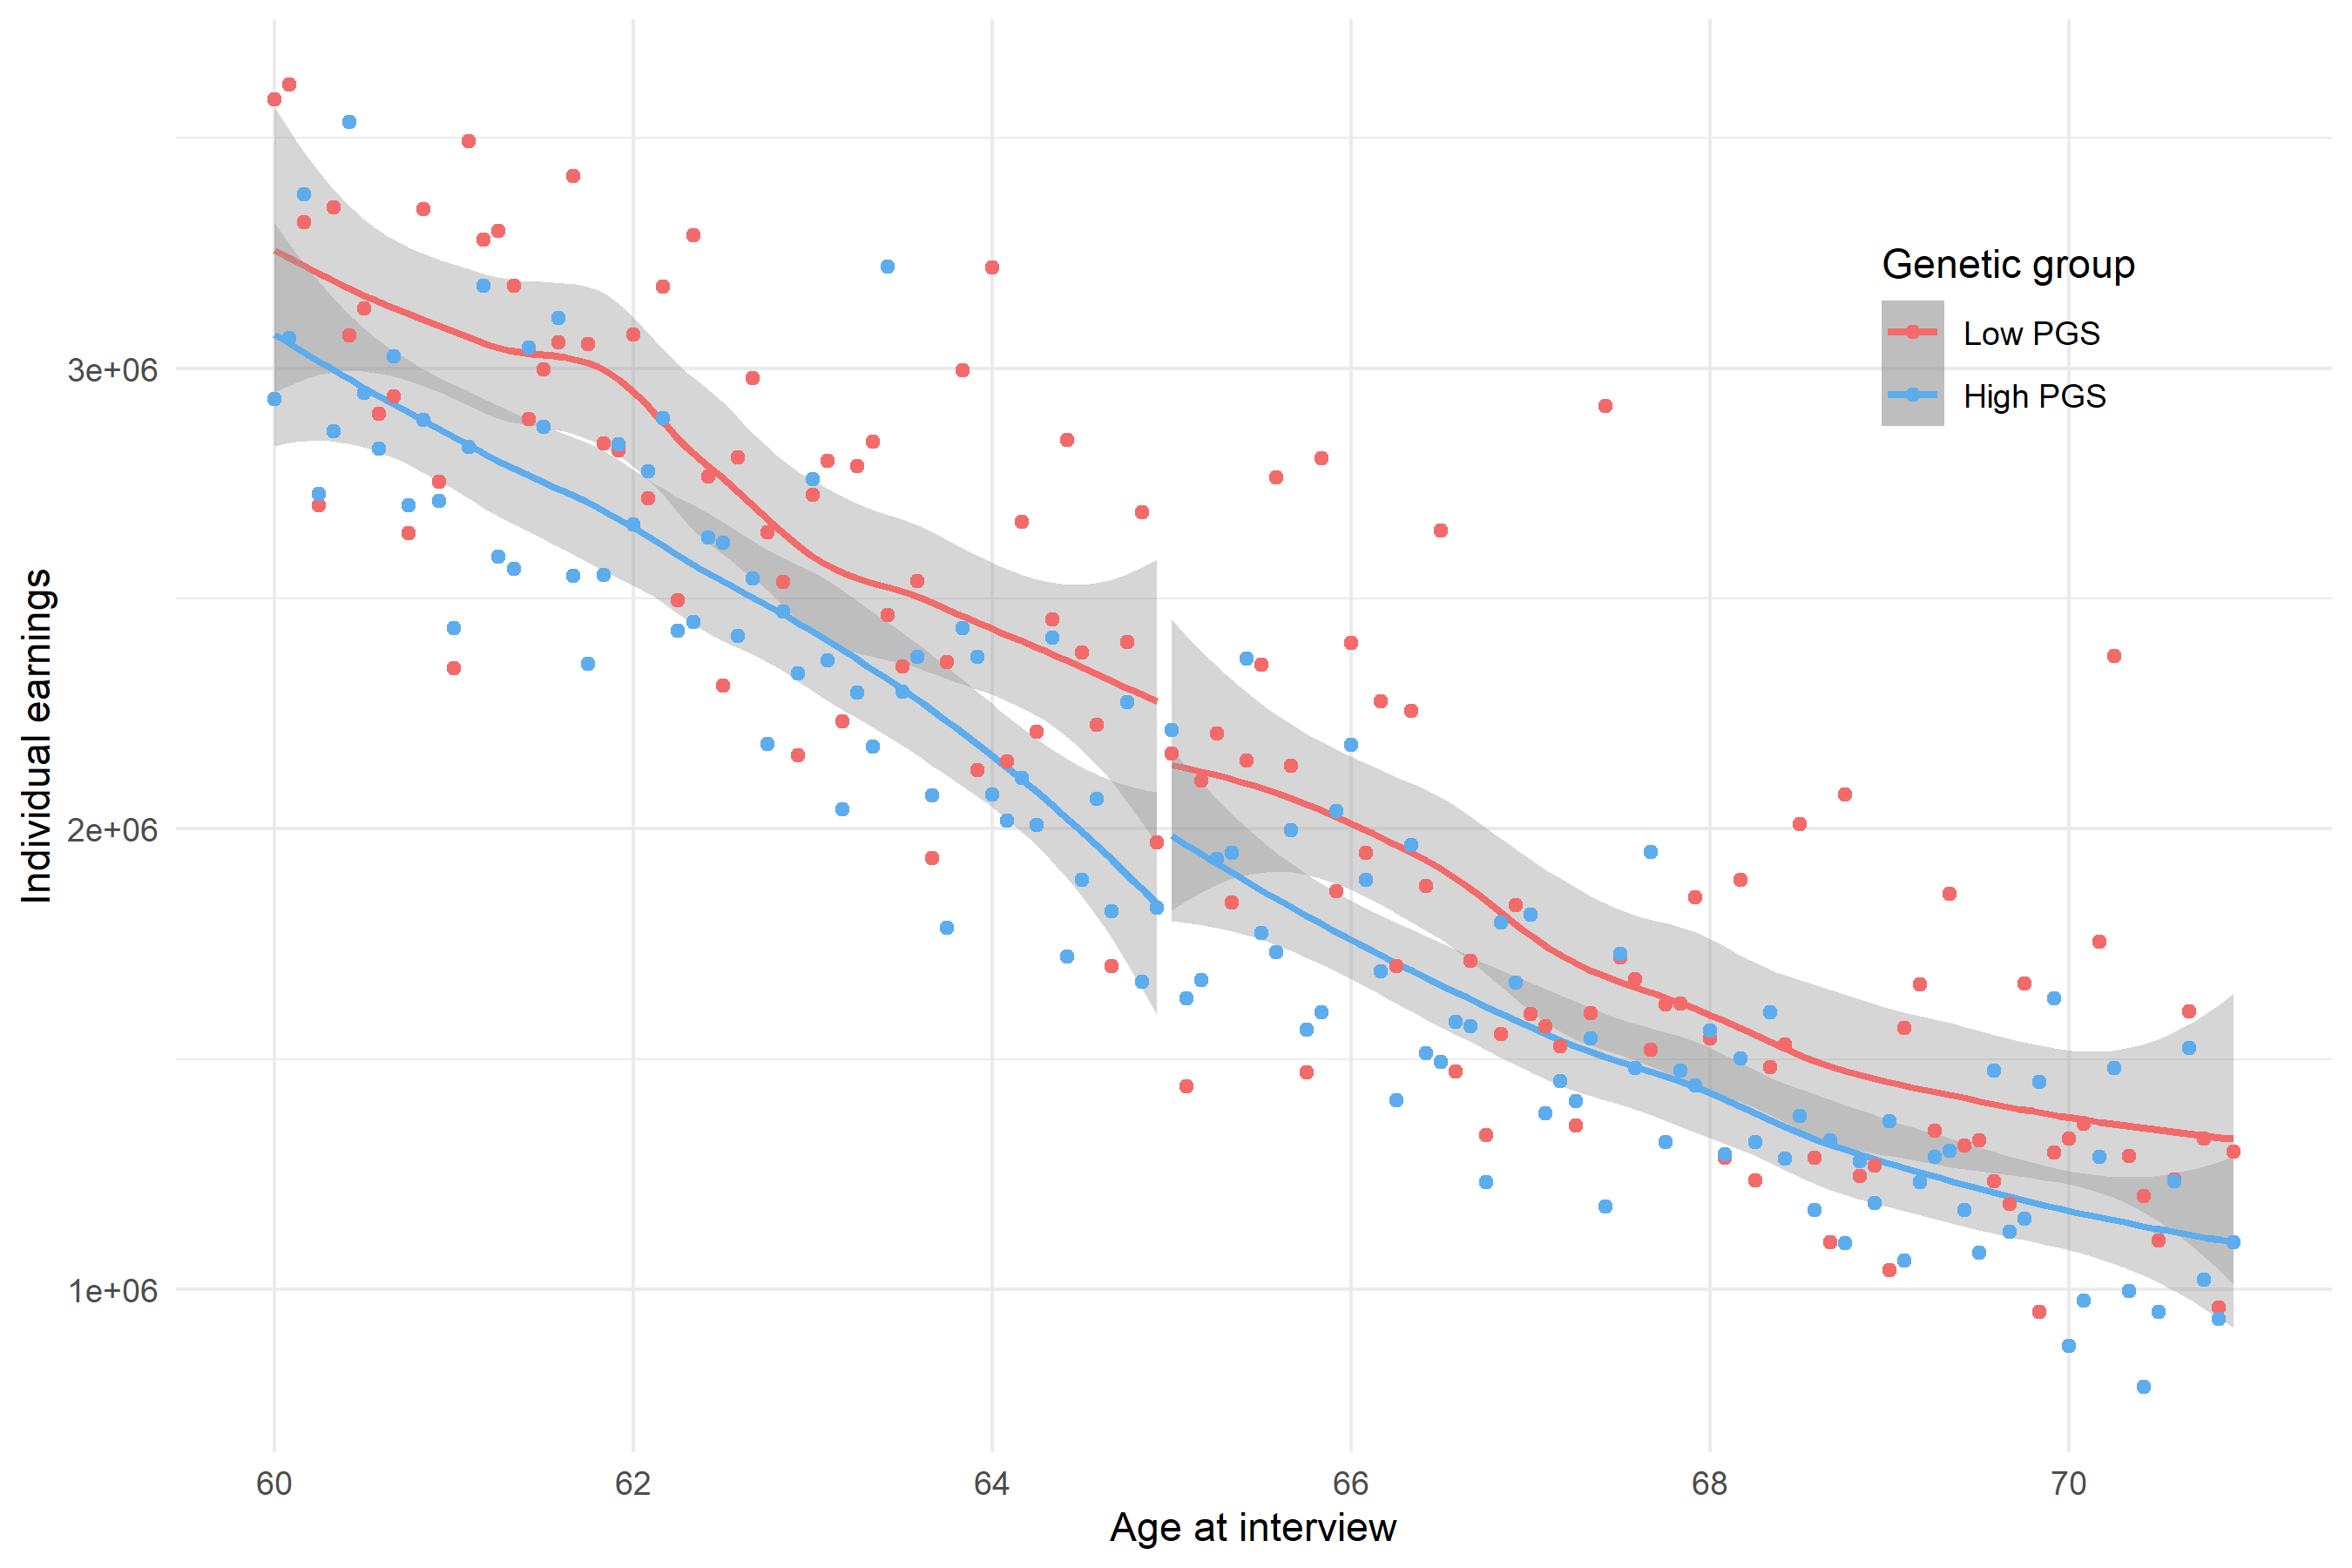
\includegraphics[width=.36\textwidth]{../../3_output/over_time/graph_6070iearnrdd_agebypgs.png}

%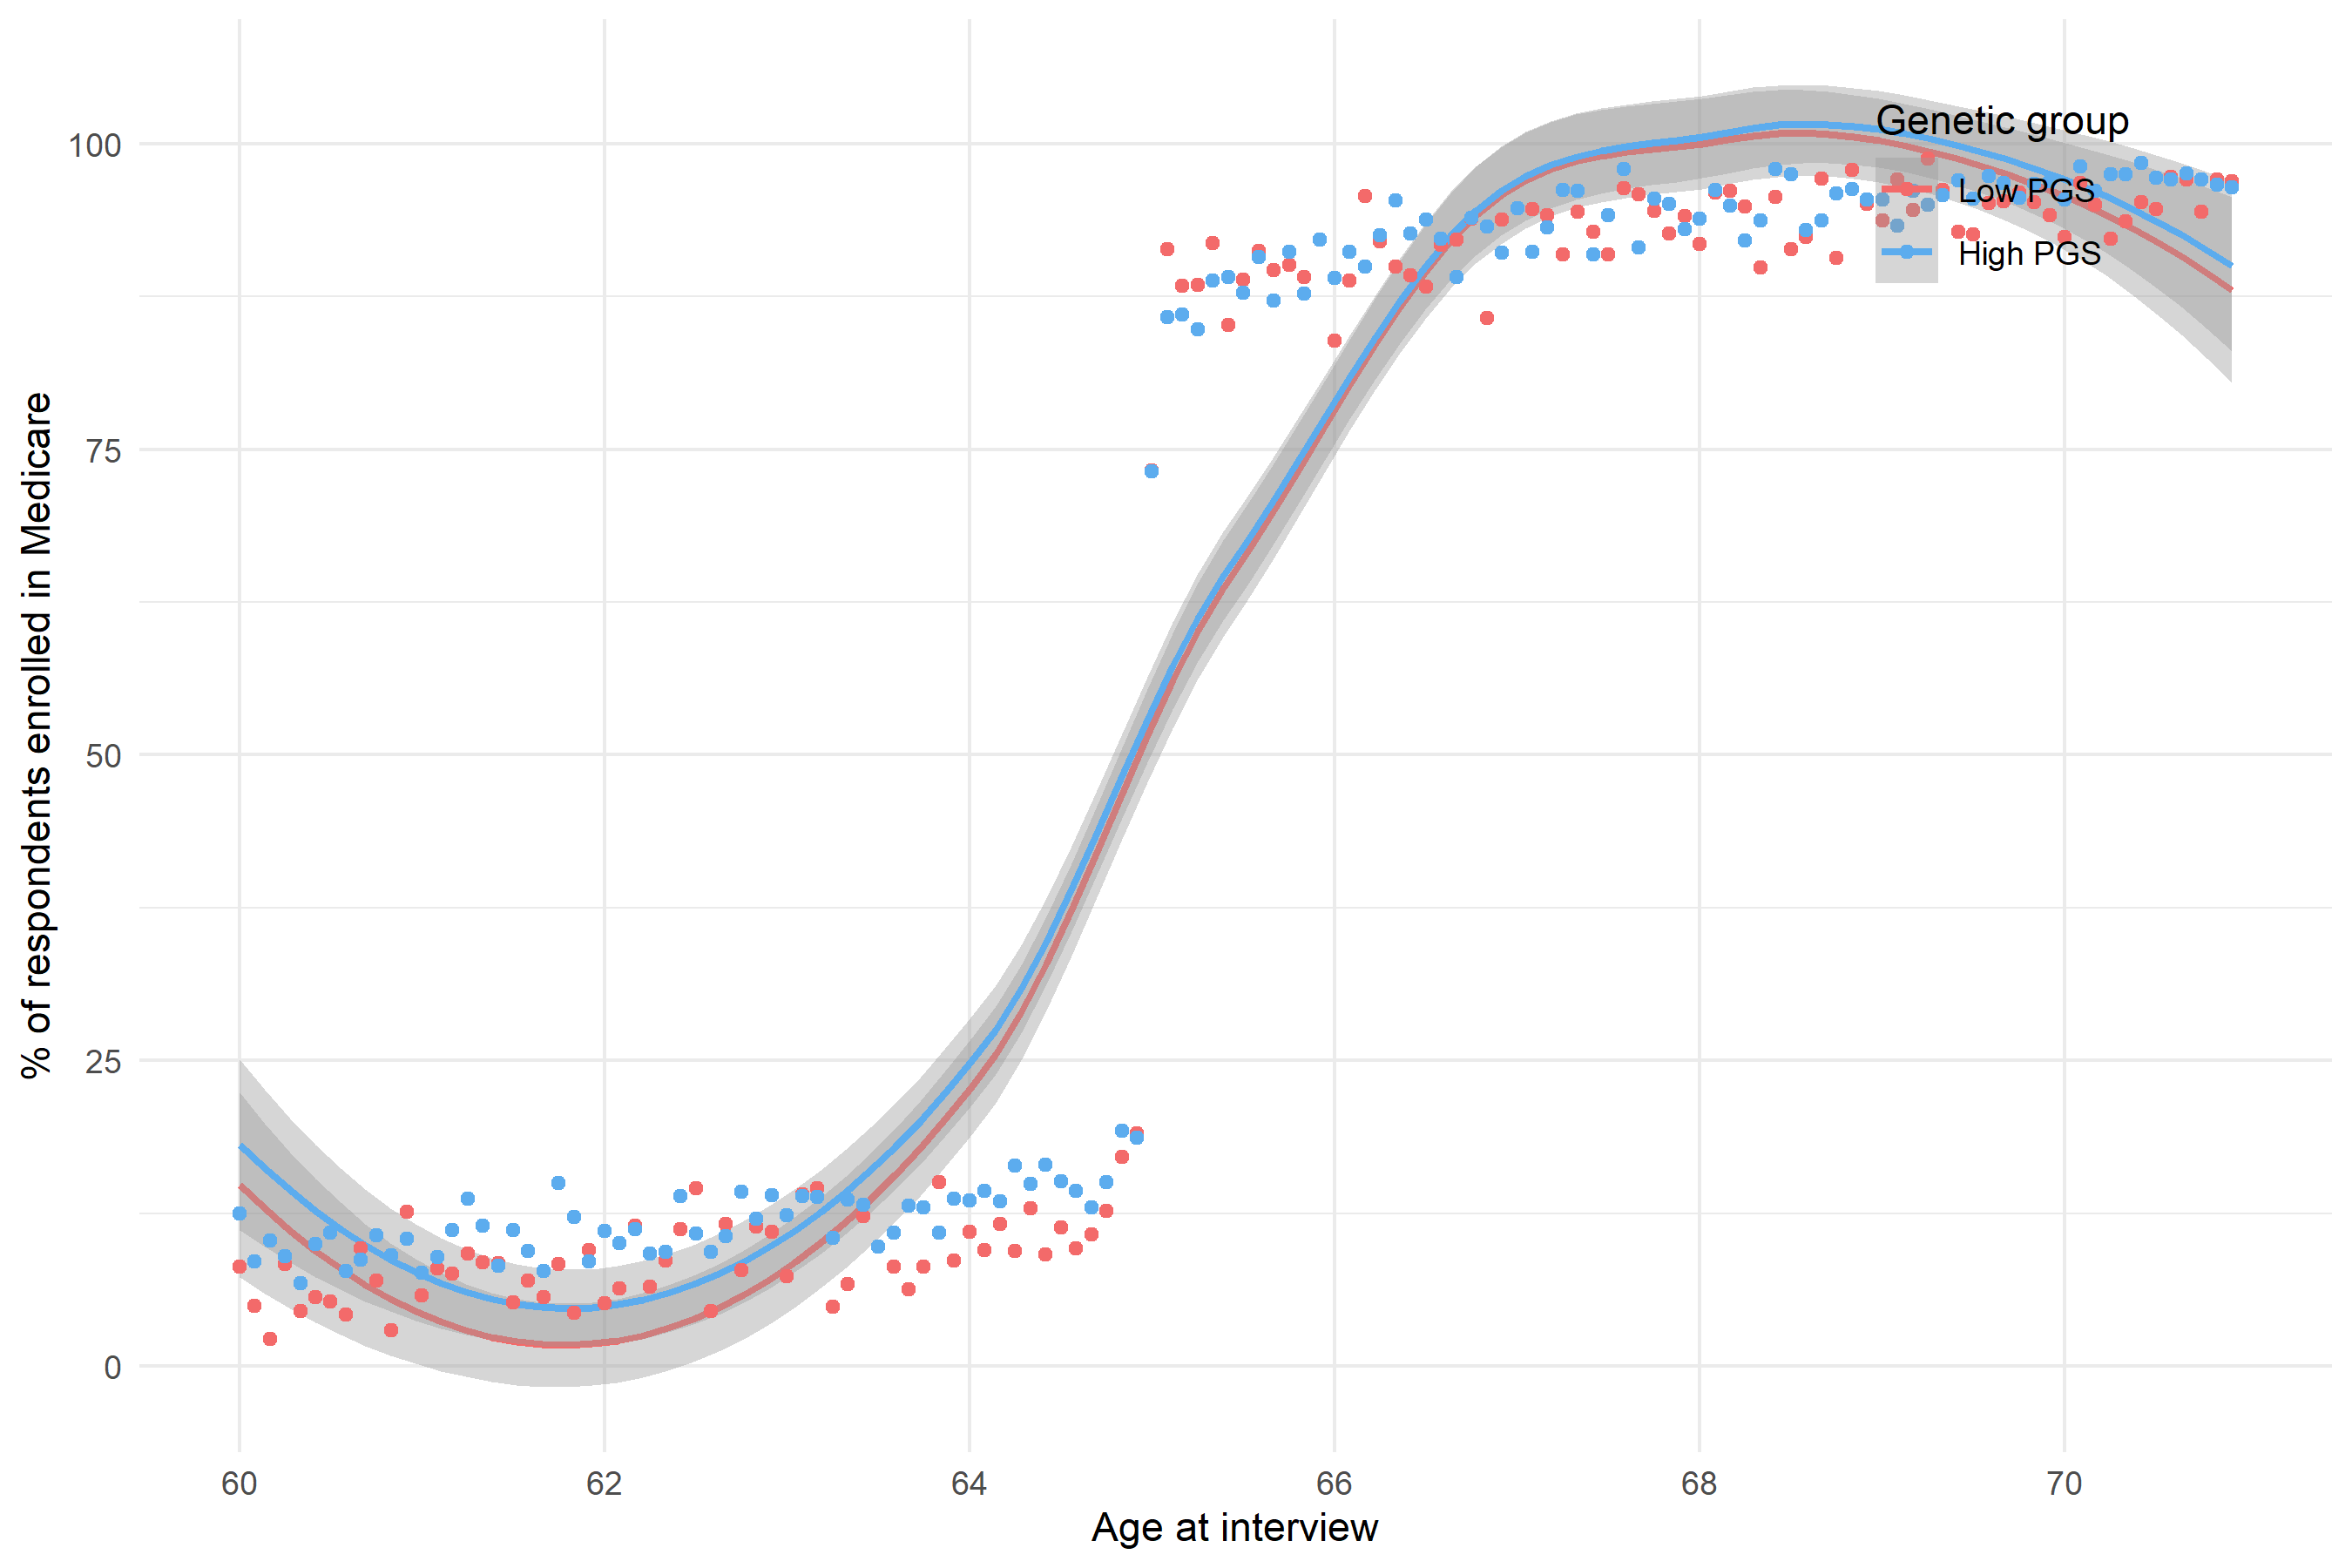
\includegraphics[width=.36\textwidth]{../../3_output/over_time/graph_6070govmrplot_agebypgs.png}%
%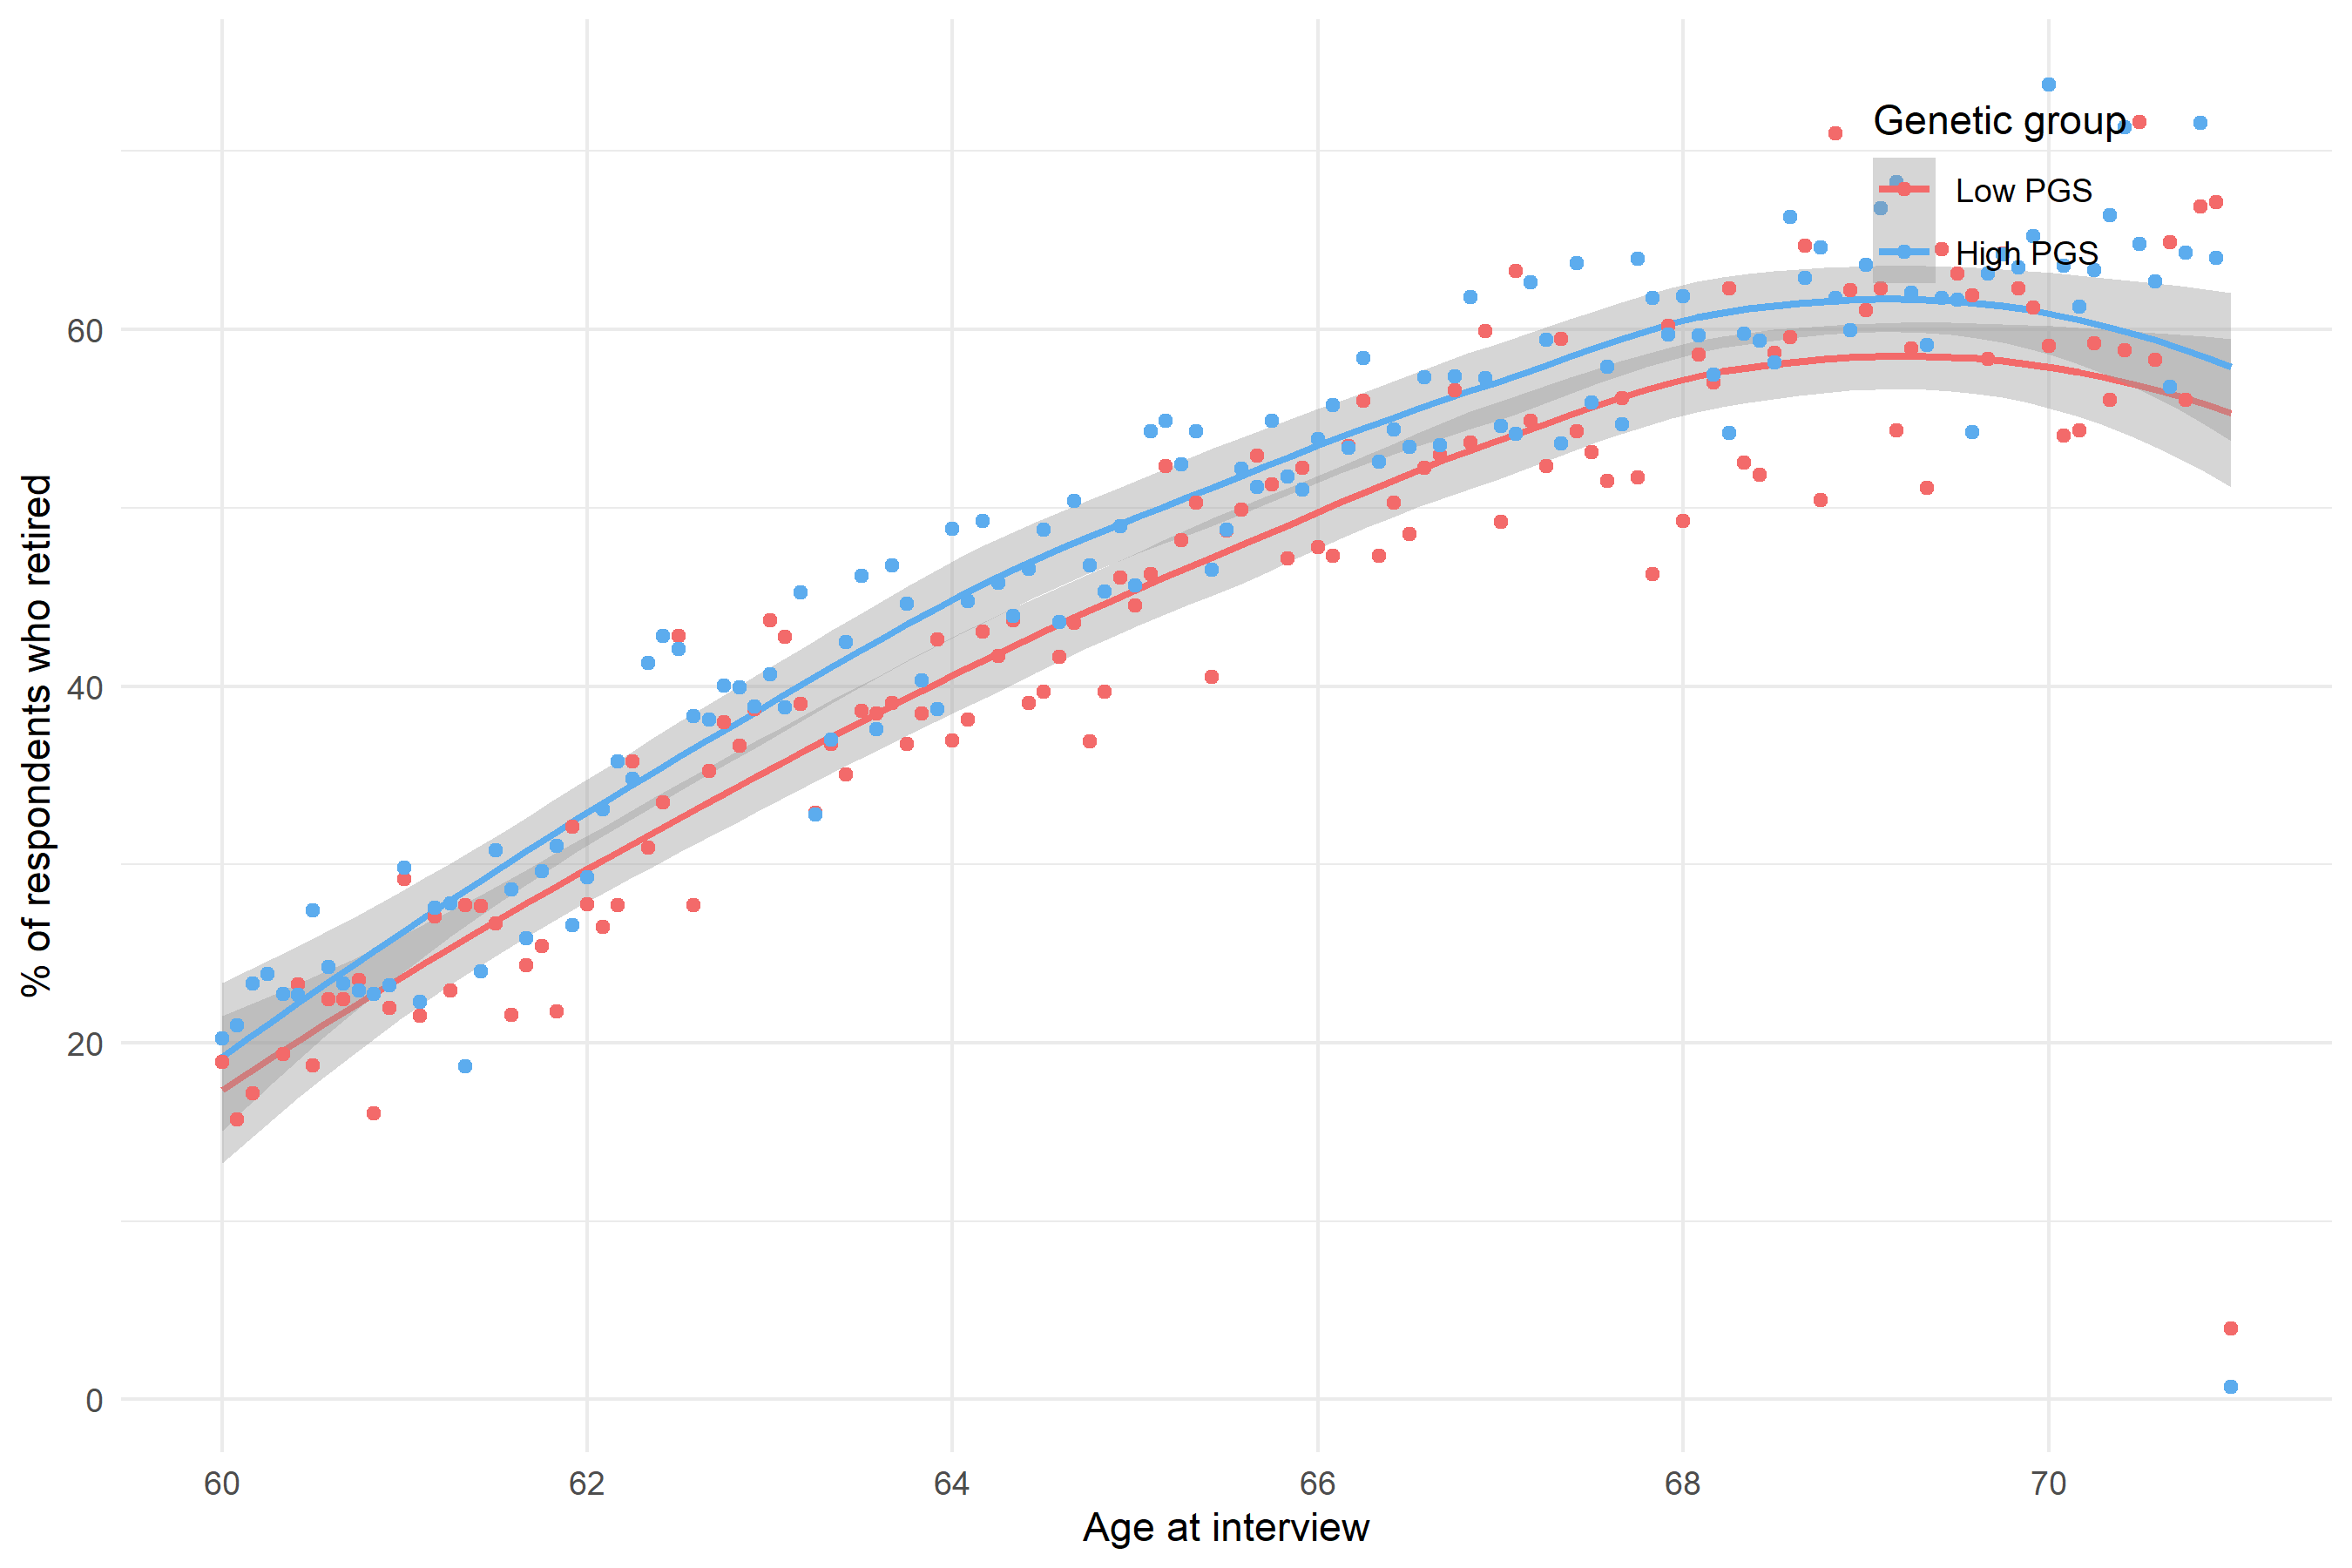
\includegraphics[width=.36\textwidth]{../../3_output/over_time/graph_6070retiredplot_agebypgs.png}%
%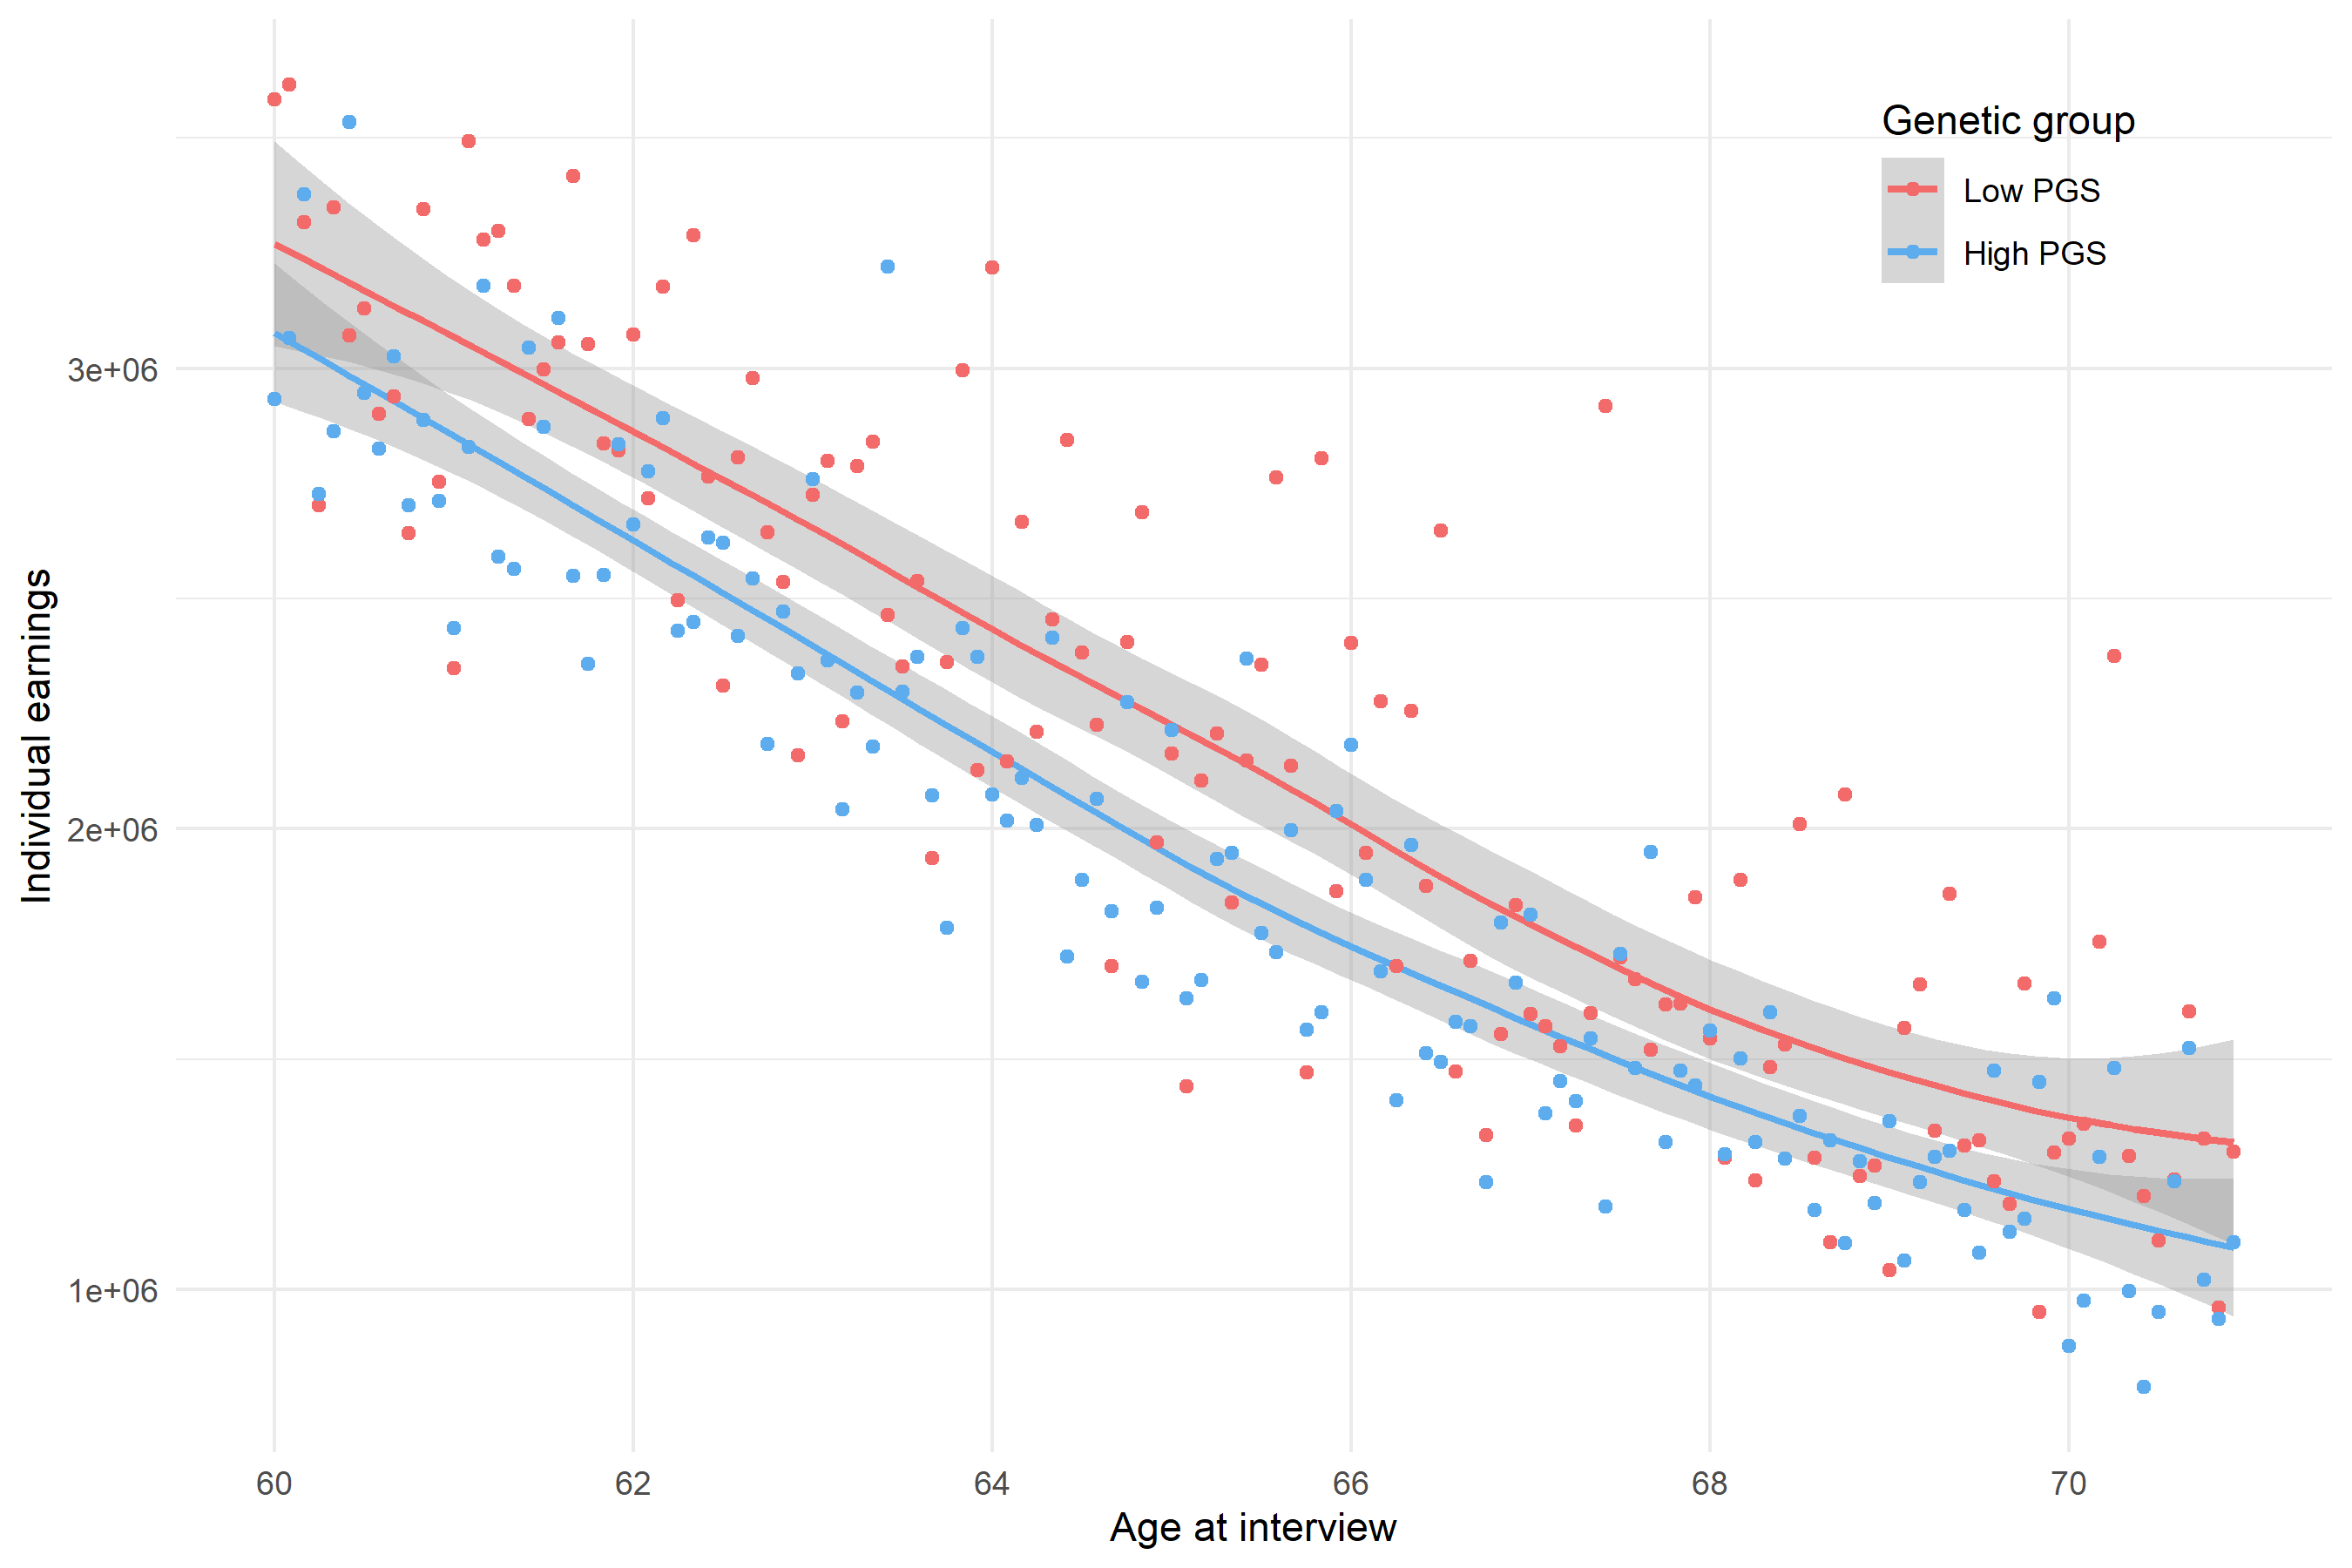
\includegraphics[width=.36\textwidth]{../../3_output/over_time/graph_6070iearnplot_agebypgs.png}

\end{frame}

%--------------------------------------------------------------%
\begin{frame}
\frametitle{Potential Confounders}
\label{frame:Confounders}
Check for differential response to shock on possible confounders \cite{Pei2018}
\begin{itemize}
	\item Retirement 		\hyperlink{fig:retire}{\beamergotobutton{}}
	\item Individual income \hyperlink{fig:wage}{\beamergotobutton{}}
	\item Household income	\hyperlink{fig:hhinc}{\beamergotobutton{}}
	%\item Wealth 			\hyperlink{fig:wealth}{\beamergotobutton{}}
	\item Out of pocket med. expenditure   \hyperlink{fig:oome}{\beamergotobutton{}}
	%\item Marital status 	\hyperlink{fig:married}{\beamergotobutton{}}
	\item Having a partner	\hyperlink{fig:mpart}{\beamergotobutton{}}
	\item Partner Smoking	\hyperlink{fig:smokePartner}{\beamergotobutton{}}
	\item Mortality \hyperlink{fig:dead2}{\beamergotobutton{2y}} \hyperlink{fig:dead5}{\beamergotobutton{5y}}
\end{itemize}

\end{frame}

%--------------------------------------------------------------% retire
\begin{frame}
\frametitle{Retirement: not likely a Confounder}
Coefficient plot of the effect of the shock on being retired.
\begin{figure}[hbtp]
\centering
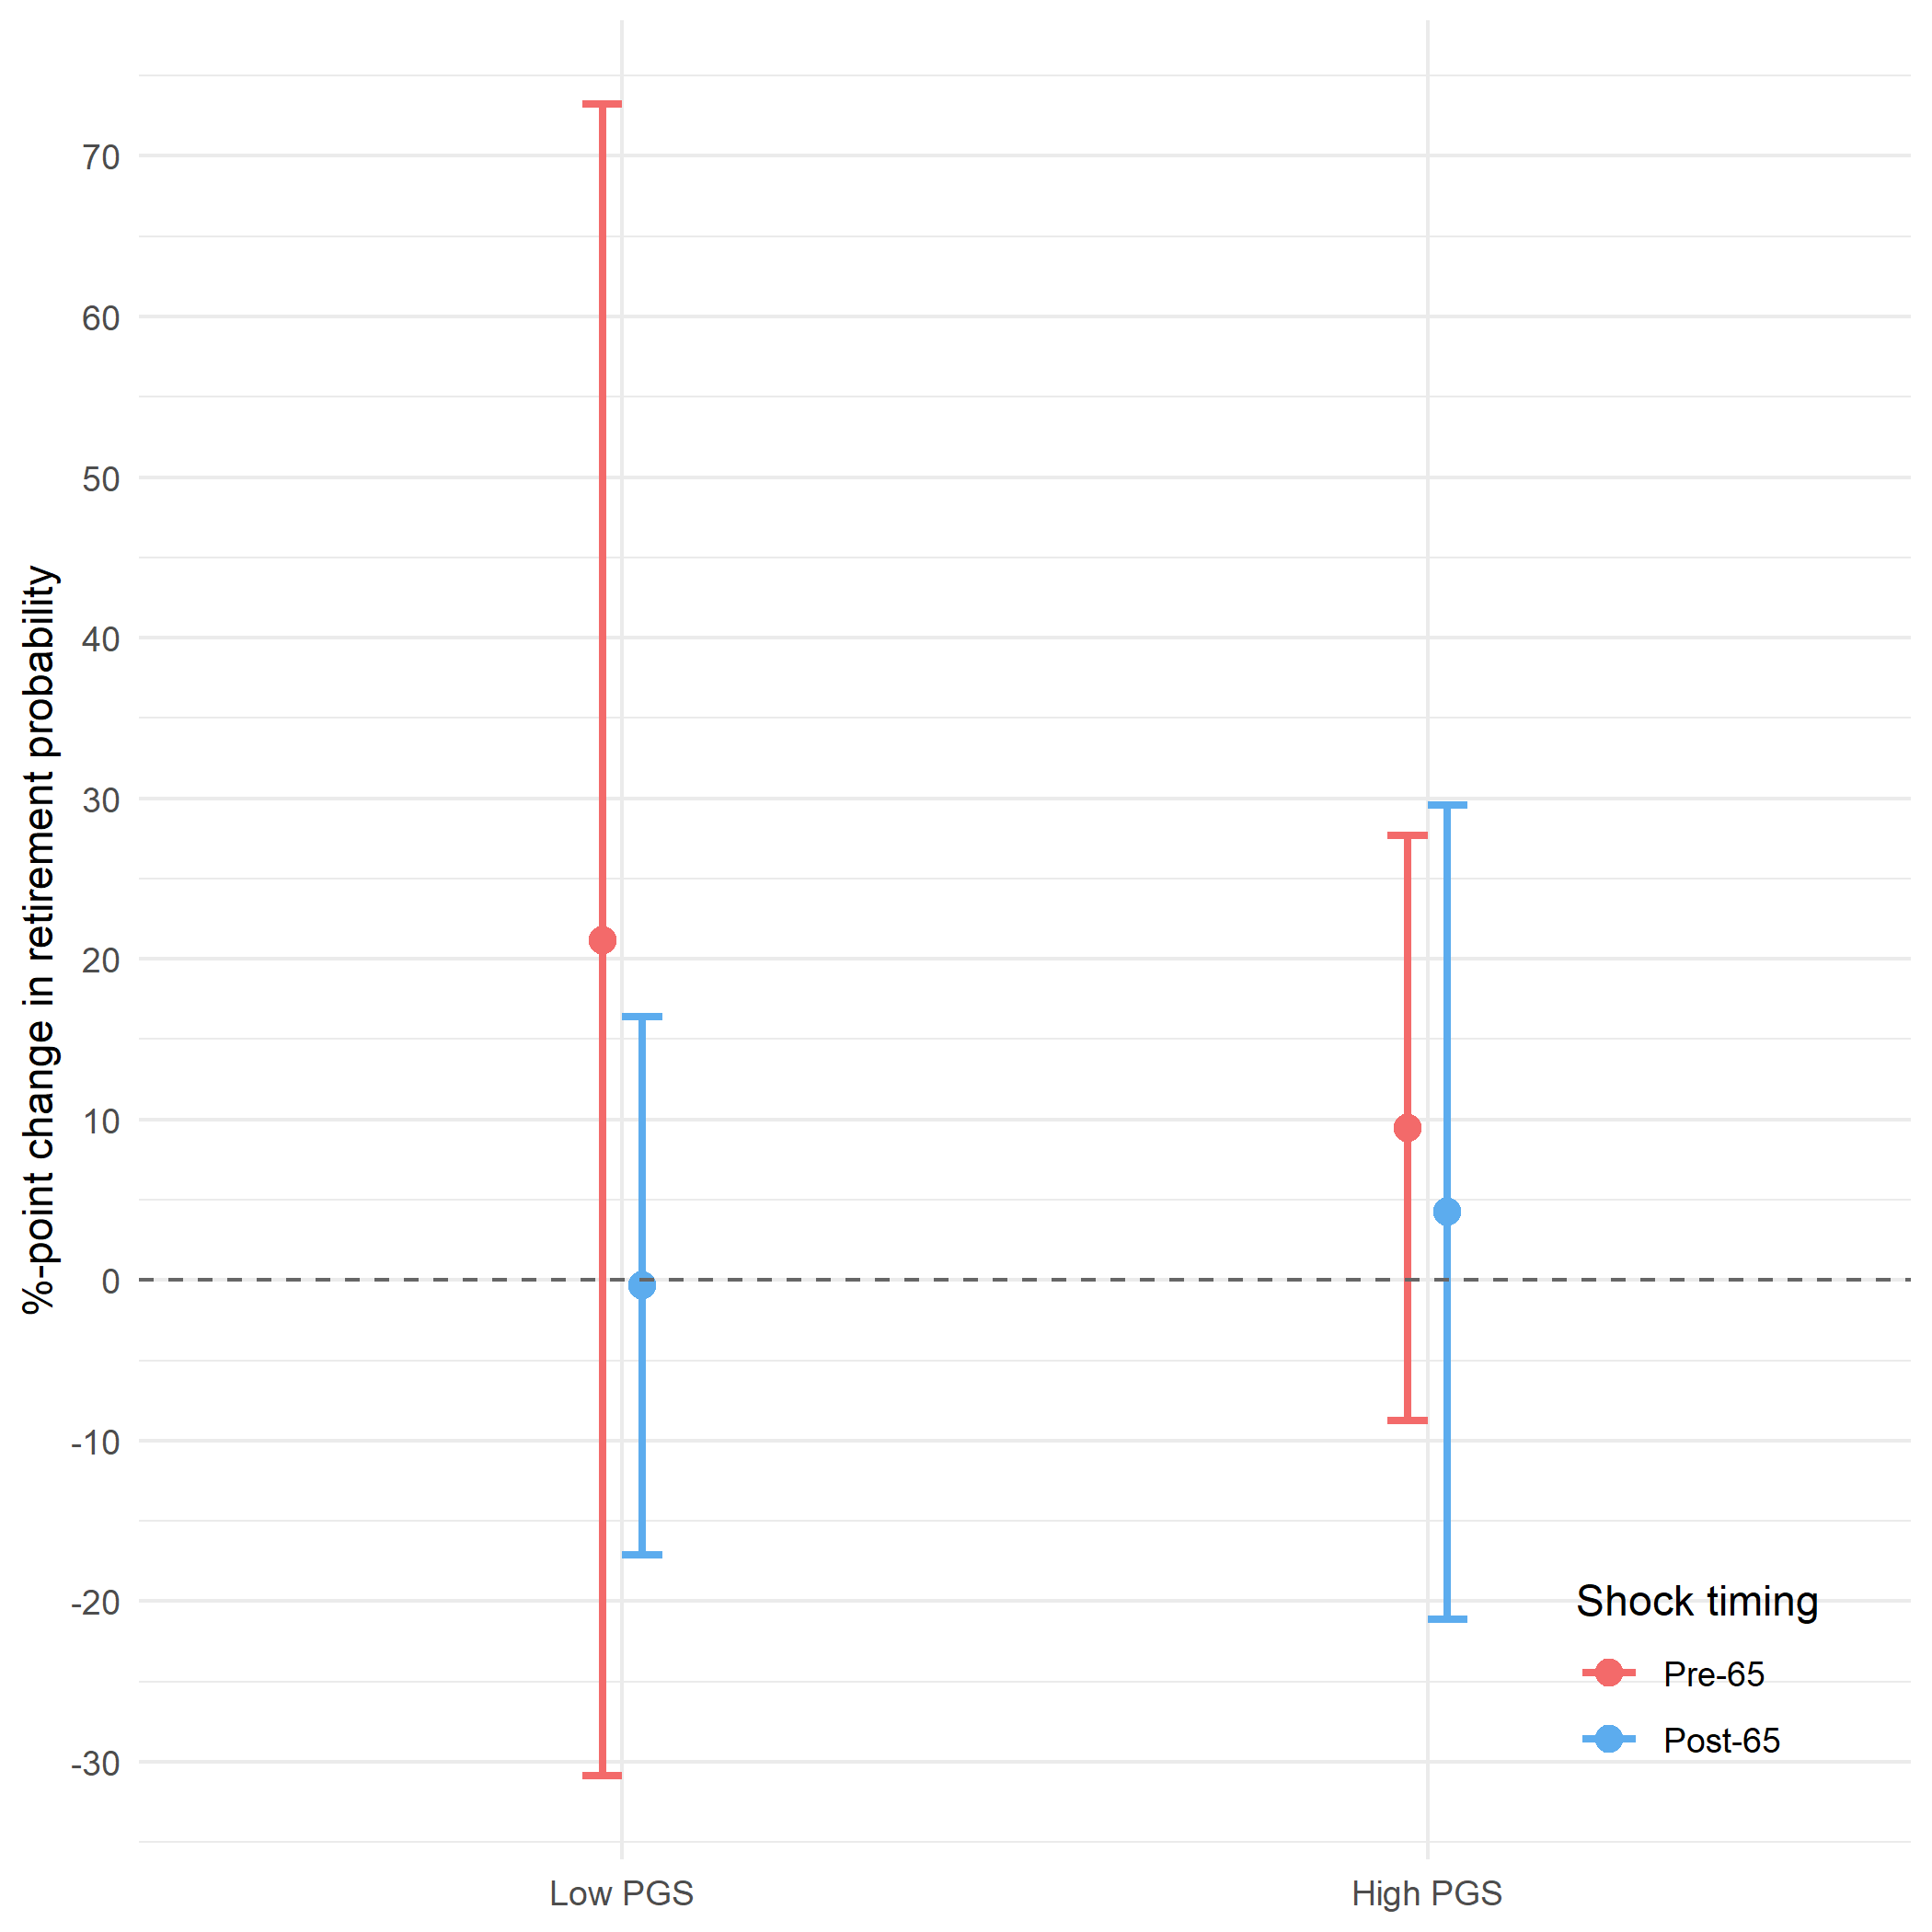
\includegraphics[height=0.8\textheight]{../../3_output/shock_effects/retired_6070_100_cv.png}
\label{fig:retire}
\end{figure}
%\hyperlink{frame:robustness}{\beamergotobutton{back}}
\end{frame}

%--------------------------------------------------------------% wage
\begin{frame}
\frametitle{Wage: not likely a Confounder}
Coefficient plot of the effect of the shock on log reported earnings.
\begin{figure}[hbtp]
\centering
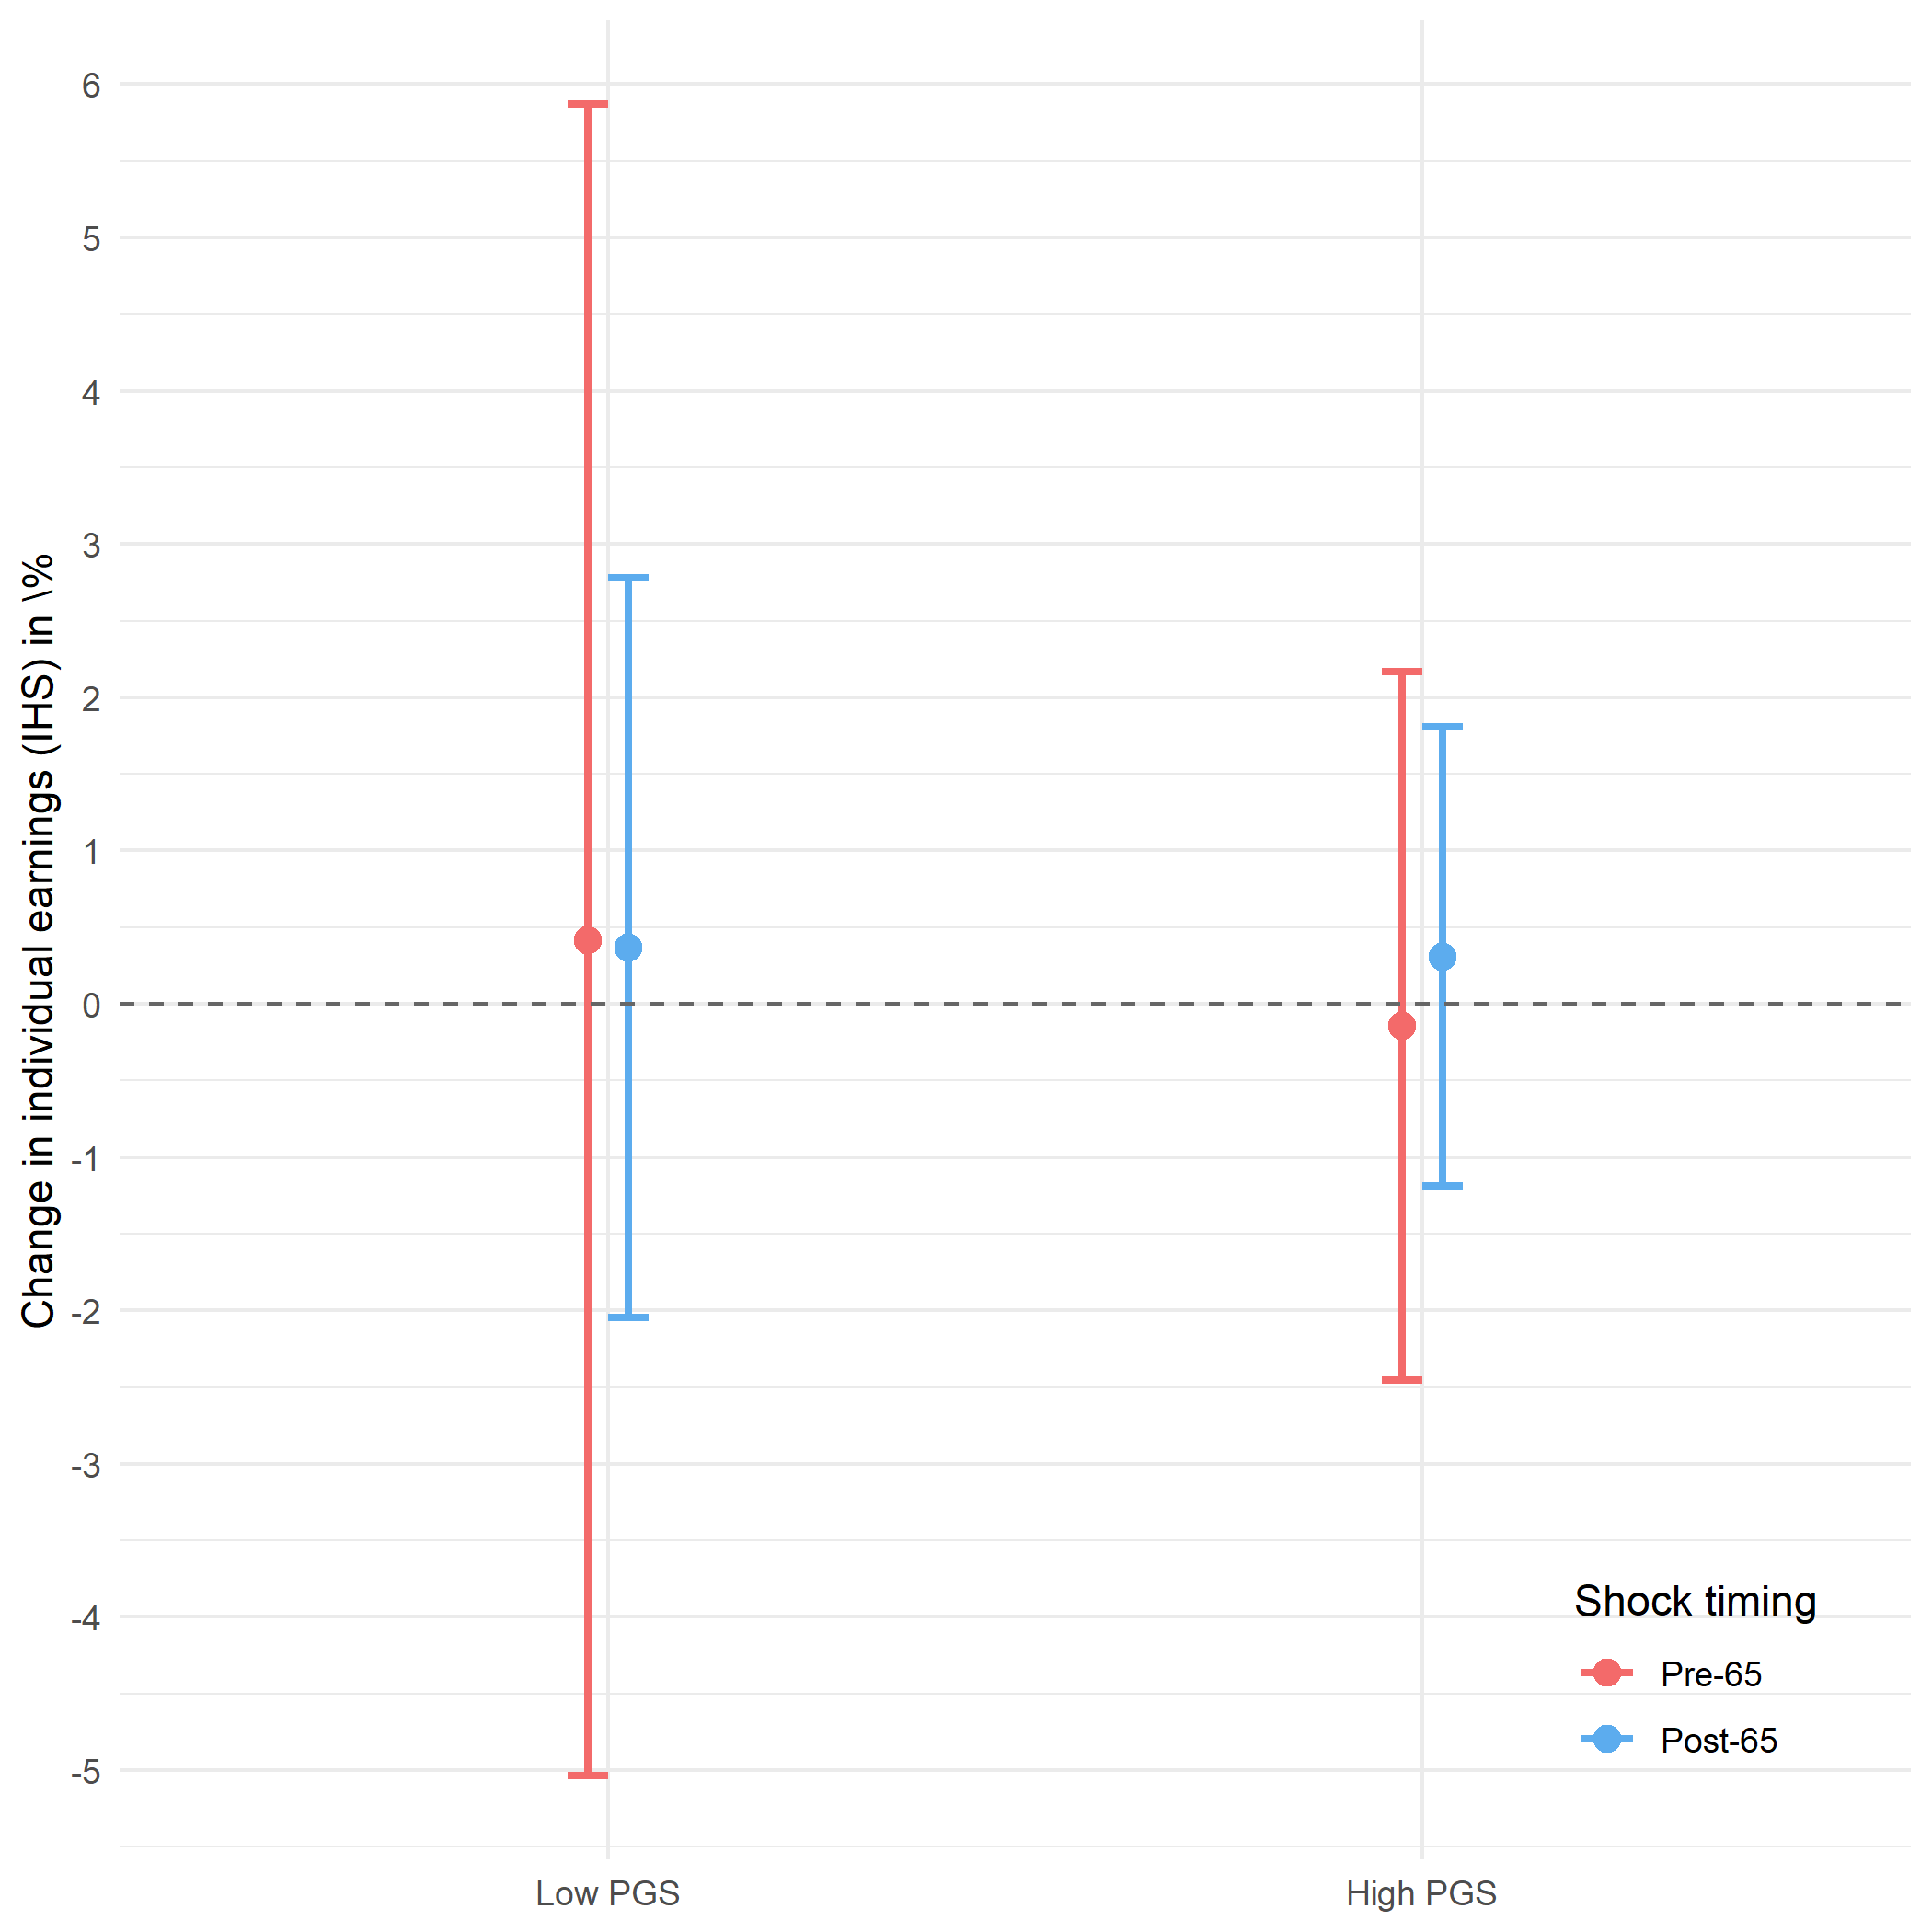
\includegraphics[height=0.8\textheight]{../../3_output/shock_effects/IHSwage_6070_100_cv.png}
\label{fig:wage}
\end{figure}
%\hyperlink{frame:robustness}{\beamergotobutton{back}}
\end{frame}

%--------------------------------------------------------------% hhinc
\begin{frame}
\frametitle{Household Income: not likely a Confounder}
Coefficient plot of the effect of the shock on household income.
\begin{figure}[hbtp]
\centering
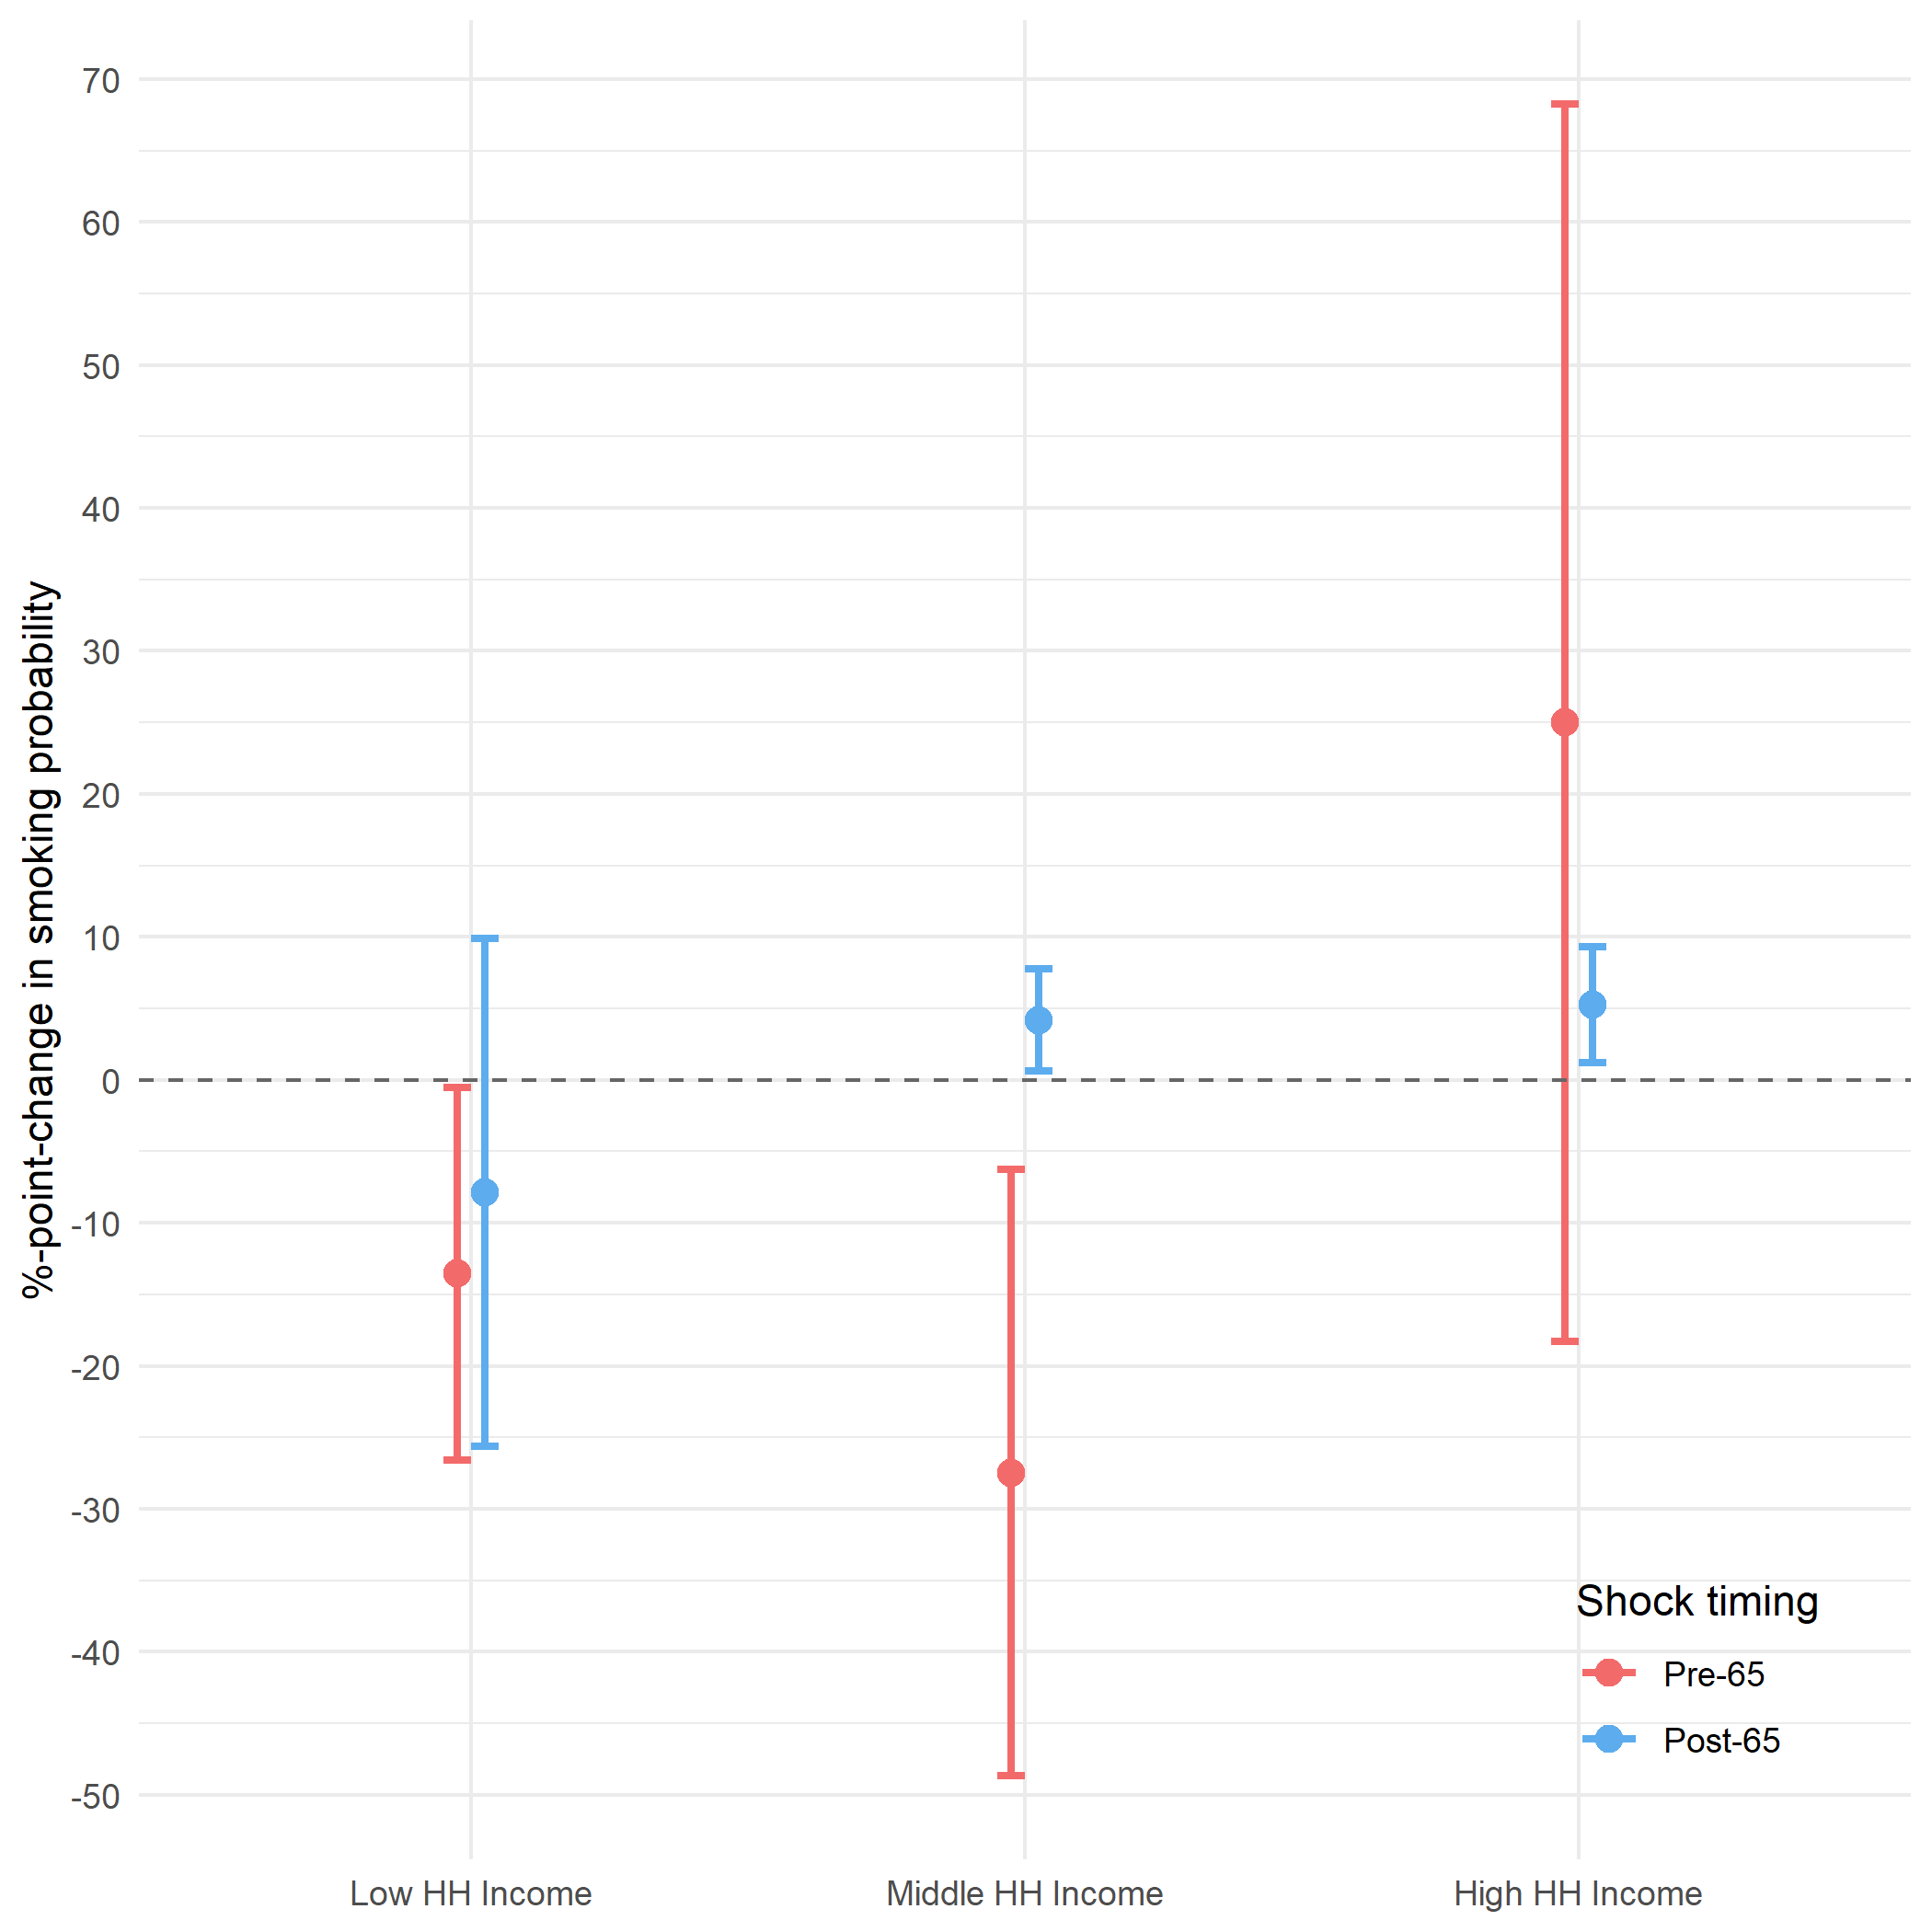
\includegraphics[height=0.8\textheight]{../../3_output/shock_effects/hhinc_6070_100_cv.png}
\label{fig:hhinc}
\end{figure}
%\hyperlink{frame:robustness}{\beamergotobutton{back}}
\end{frame}

%%--------------------------------------------------------------% wealth
%\begin{frame}
%\frametitle{Wealth: possibly a Confounder?}
%Coefficient plot of the effect of the shock on household wealth.
%\begin{figure}[hbtp]
%
%\centering
%\includegraphics[height=0.8\textheight]{../../3_output/shock_effects/wealth_6070_100_cv.png}
%\label{fig:wealth}
%\end{figure}
%%\hyperlink{frame:robustness}{\beamergotobutton{back}}
%\end{frame}

%--------------------------------------------------------------% medexp
\begin{frame}
\frametitle{Medical expenditure: not likely a Confounder}
Coefficient plot of the effect of the shock on out of poket medical enxpenditure.
\begin{figure}[hbtp]

\centering
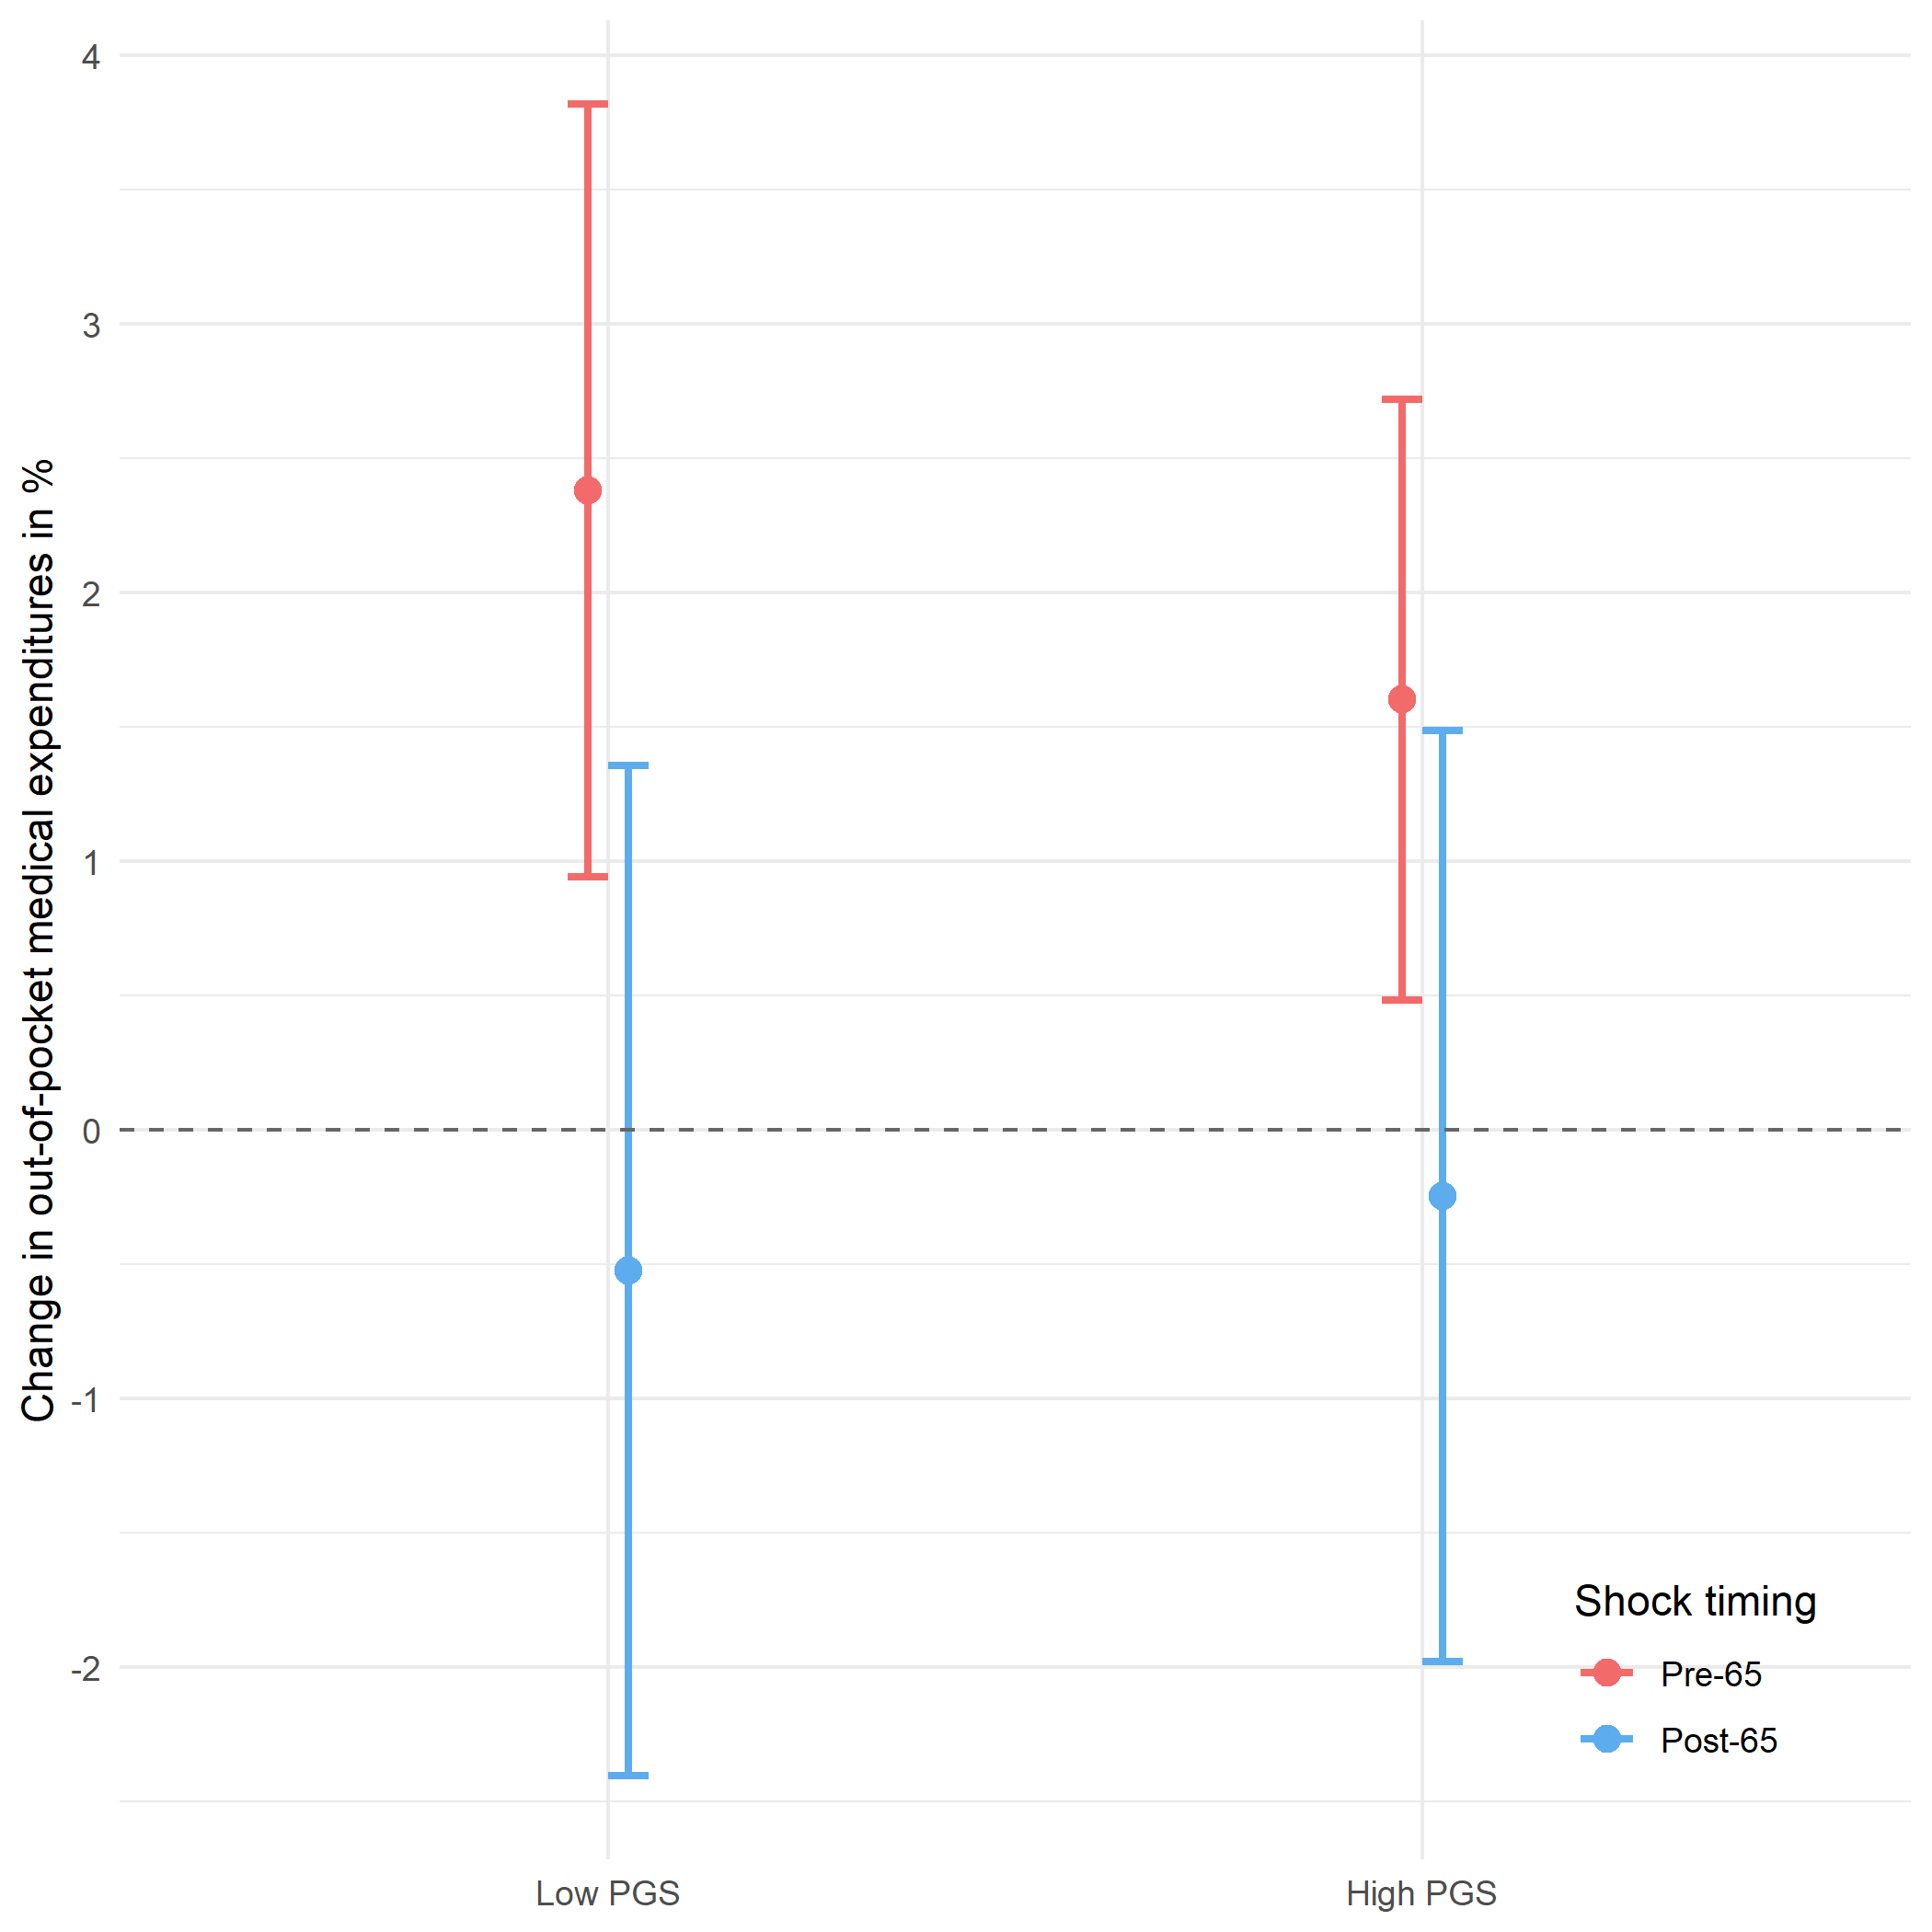
\includegraphics[height=0.8\textheight]{../../3_output/shock_effects/medexp_6070_100_cv.png}
\label{fig:medexp}
\end{figure}
%\hyperlink{frame:robustness}{\beamergotobutton{back}}
\end{frame}

%%--------------------------------------------------------------% married
%\begin{frame}
%\frametitle{Married: not likely a Confounder}
%Coefficient plot of the effect of the shock on being married.
%\begin{figure}[hbtp]
%
%\centering
%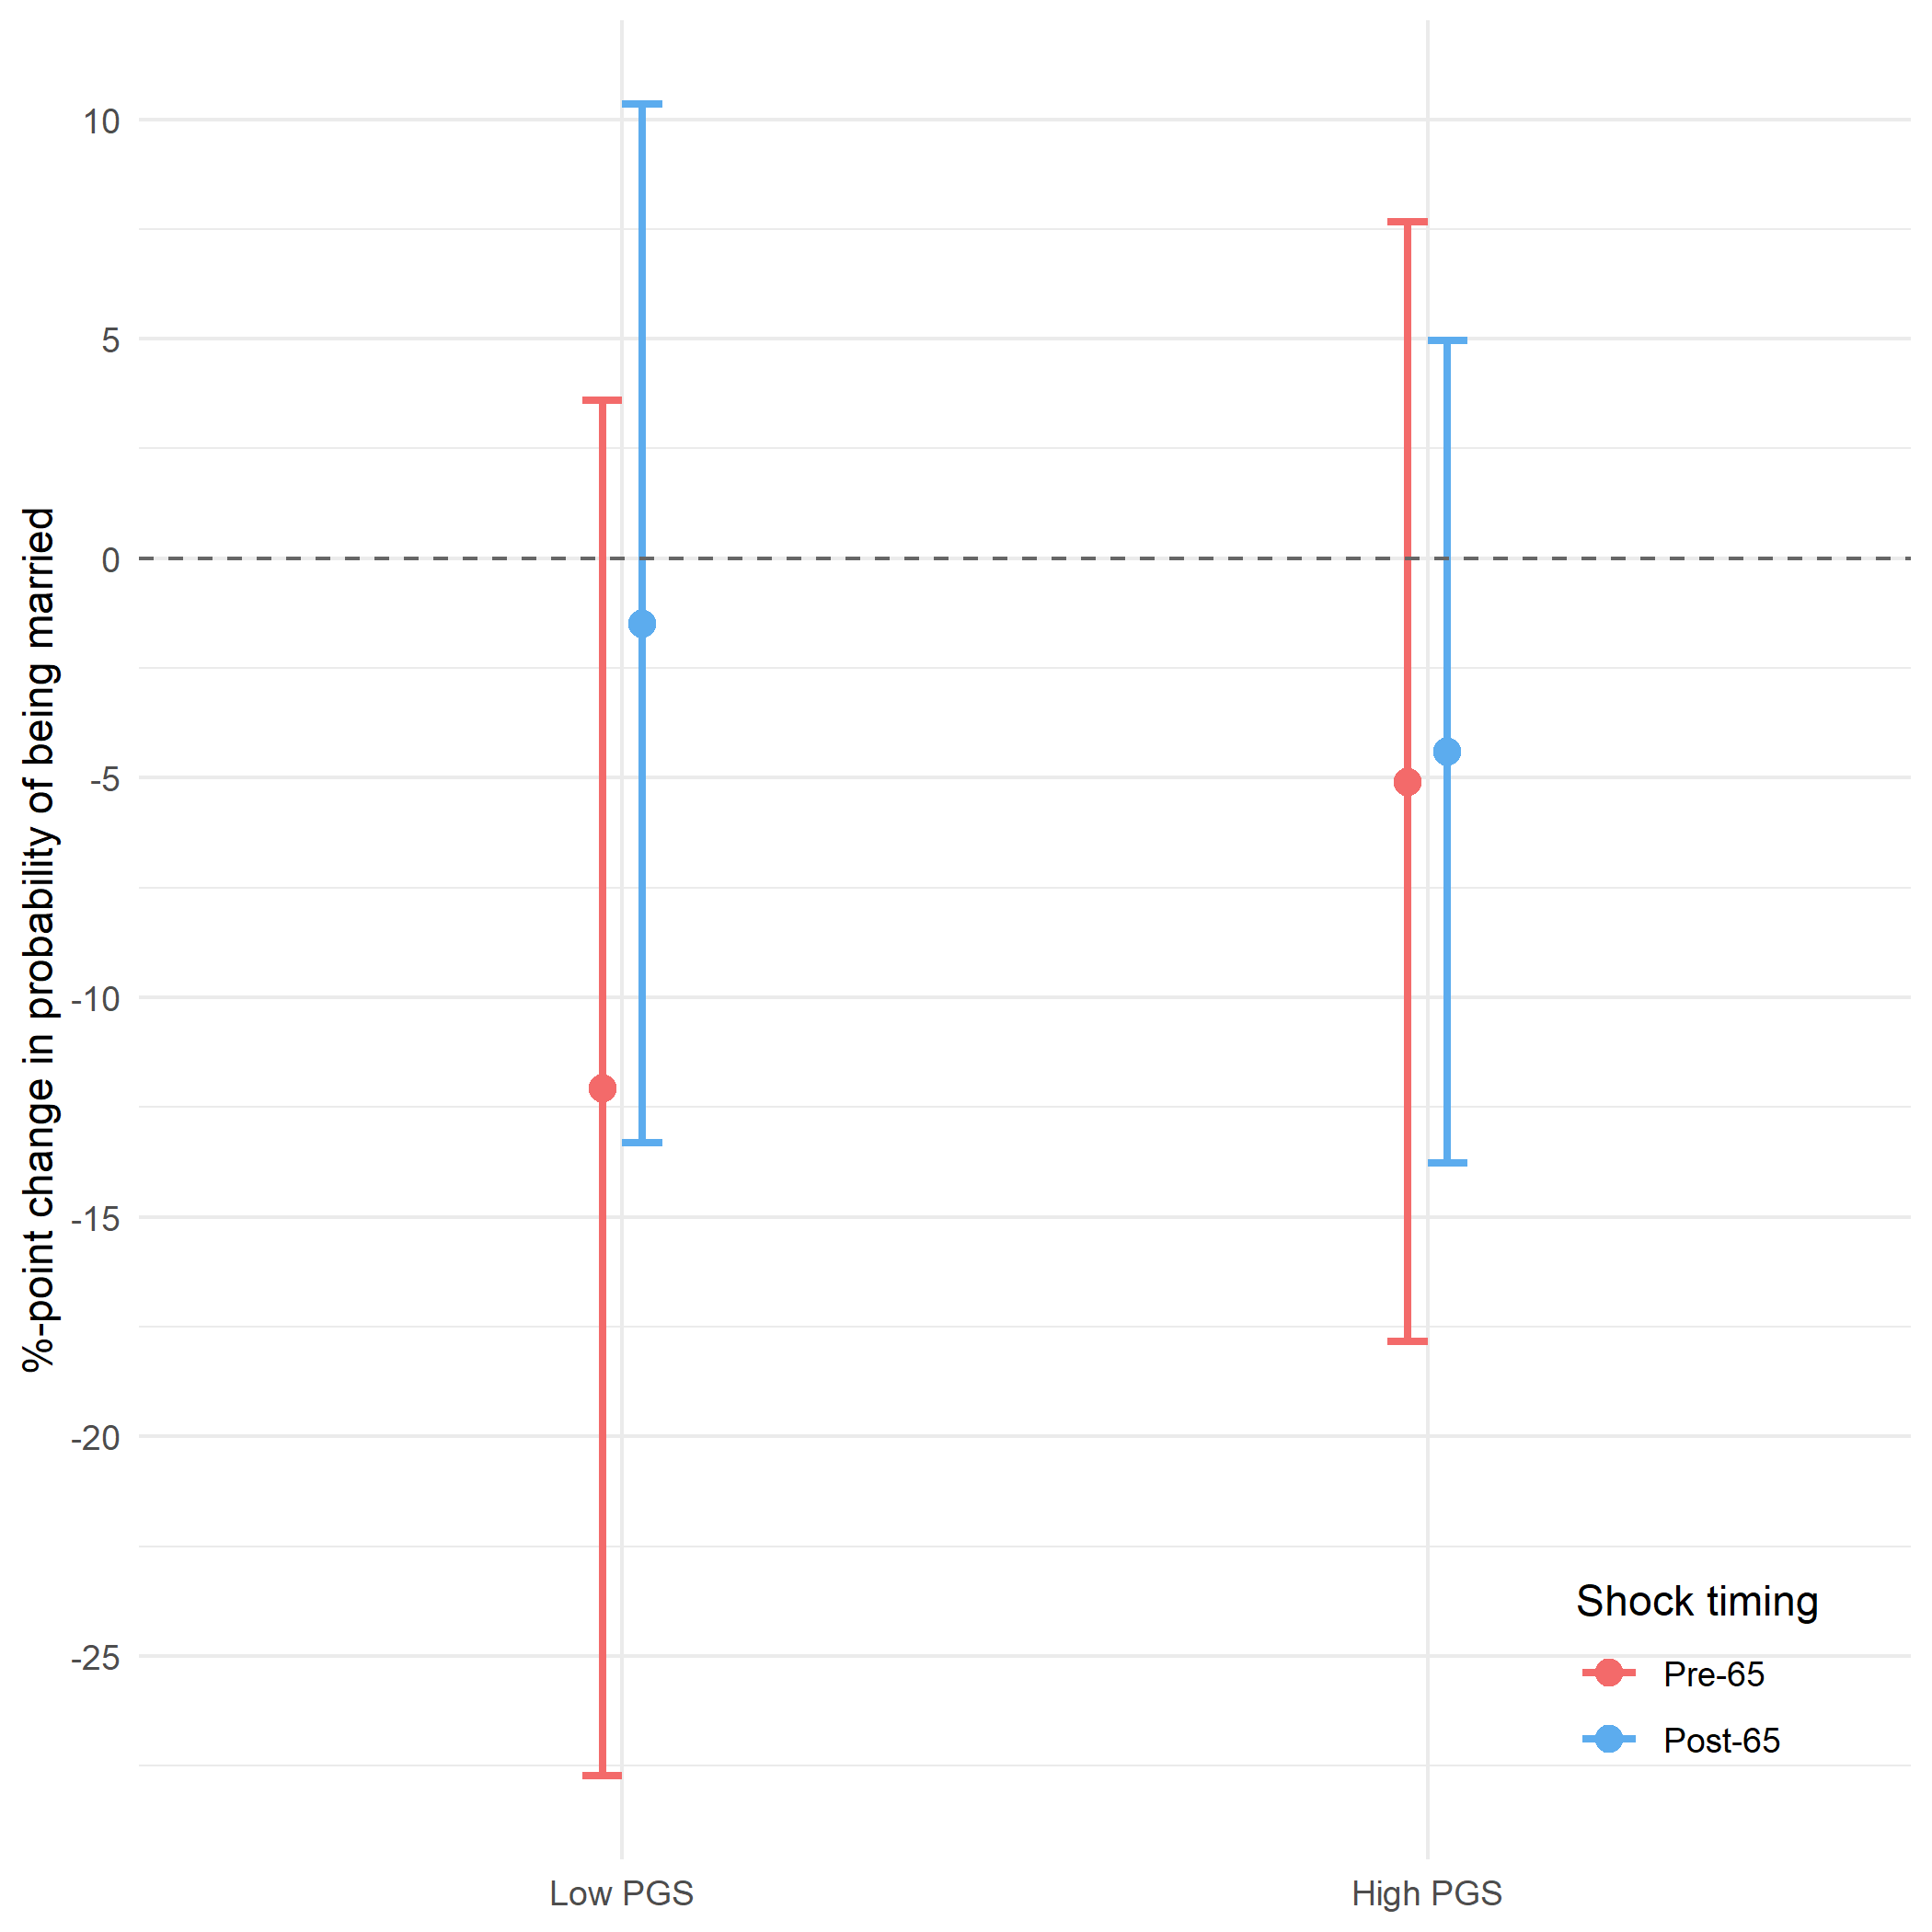
\includegraphics[height=0.8\textheight]{../../3_output/shock_effects/married_6070_100_cv.png}
%\label{fig:married}
%\end{figure}
%%\hyperlink{frame:robustness}{\beamergotobutton{back}}
%\end{frame}

%--------------------------------------------------------------% mpart
\begin{frame}
\frametitle{Having a partner: not likely a Confounder}
Coefficient plot of the effect of the shock on having a partner.
\begin{figure}[hbtp]

\centering
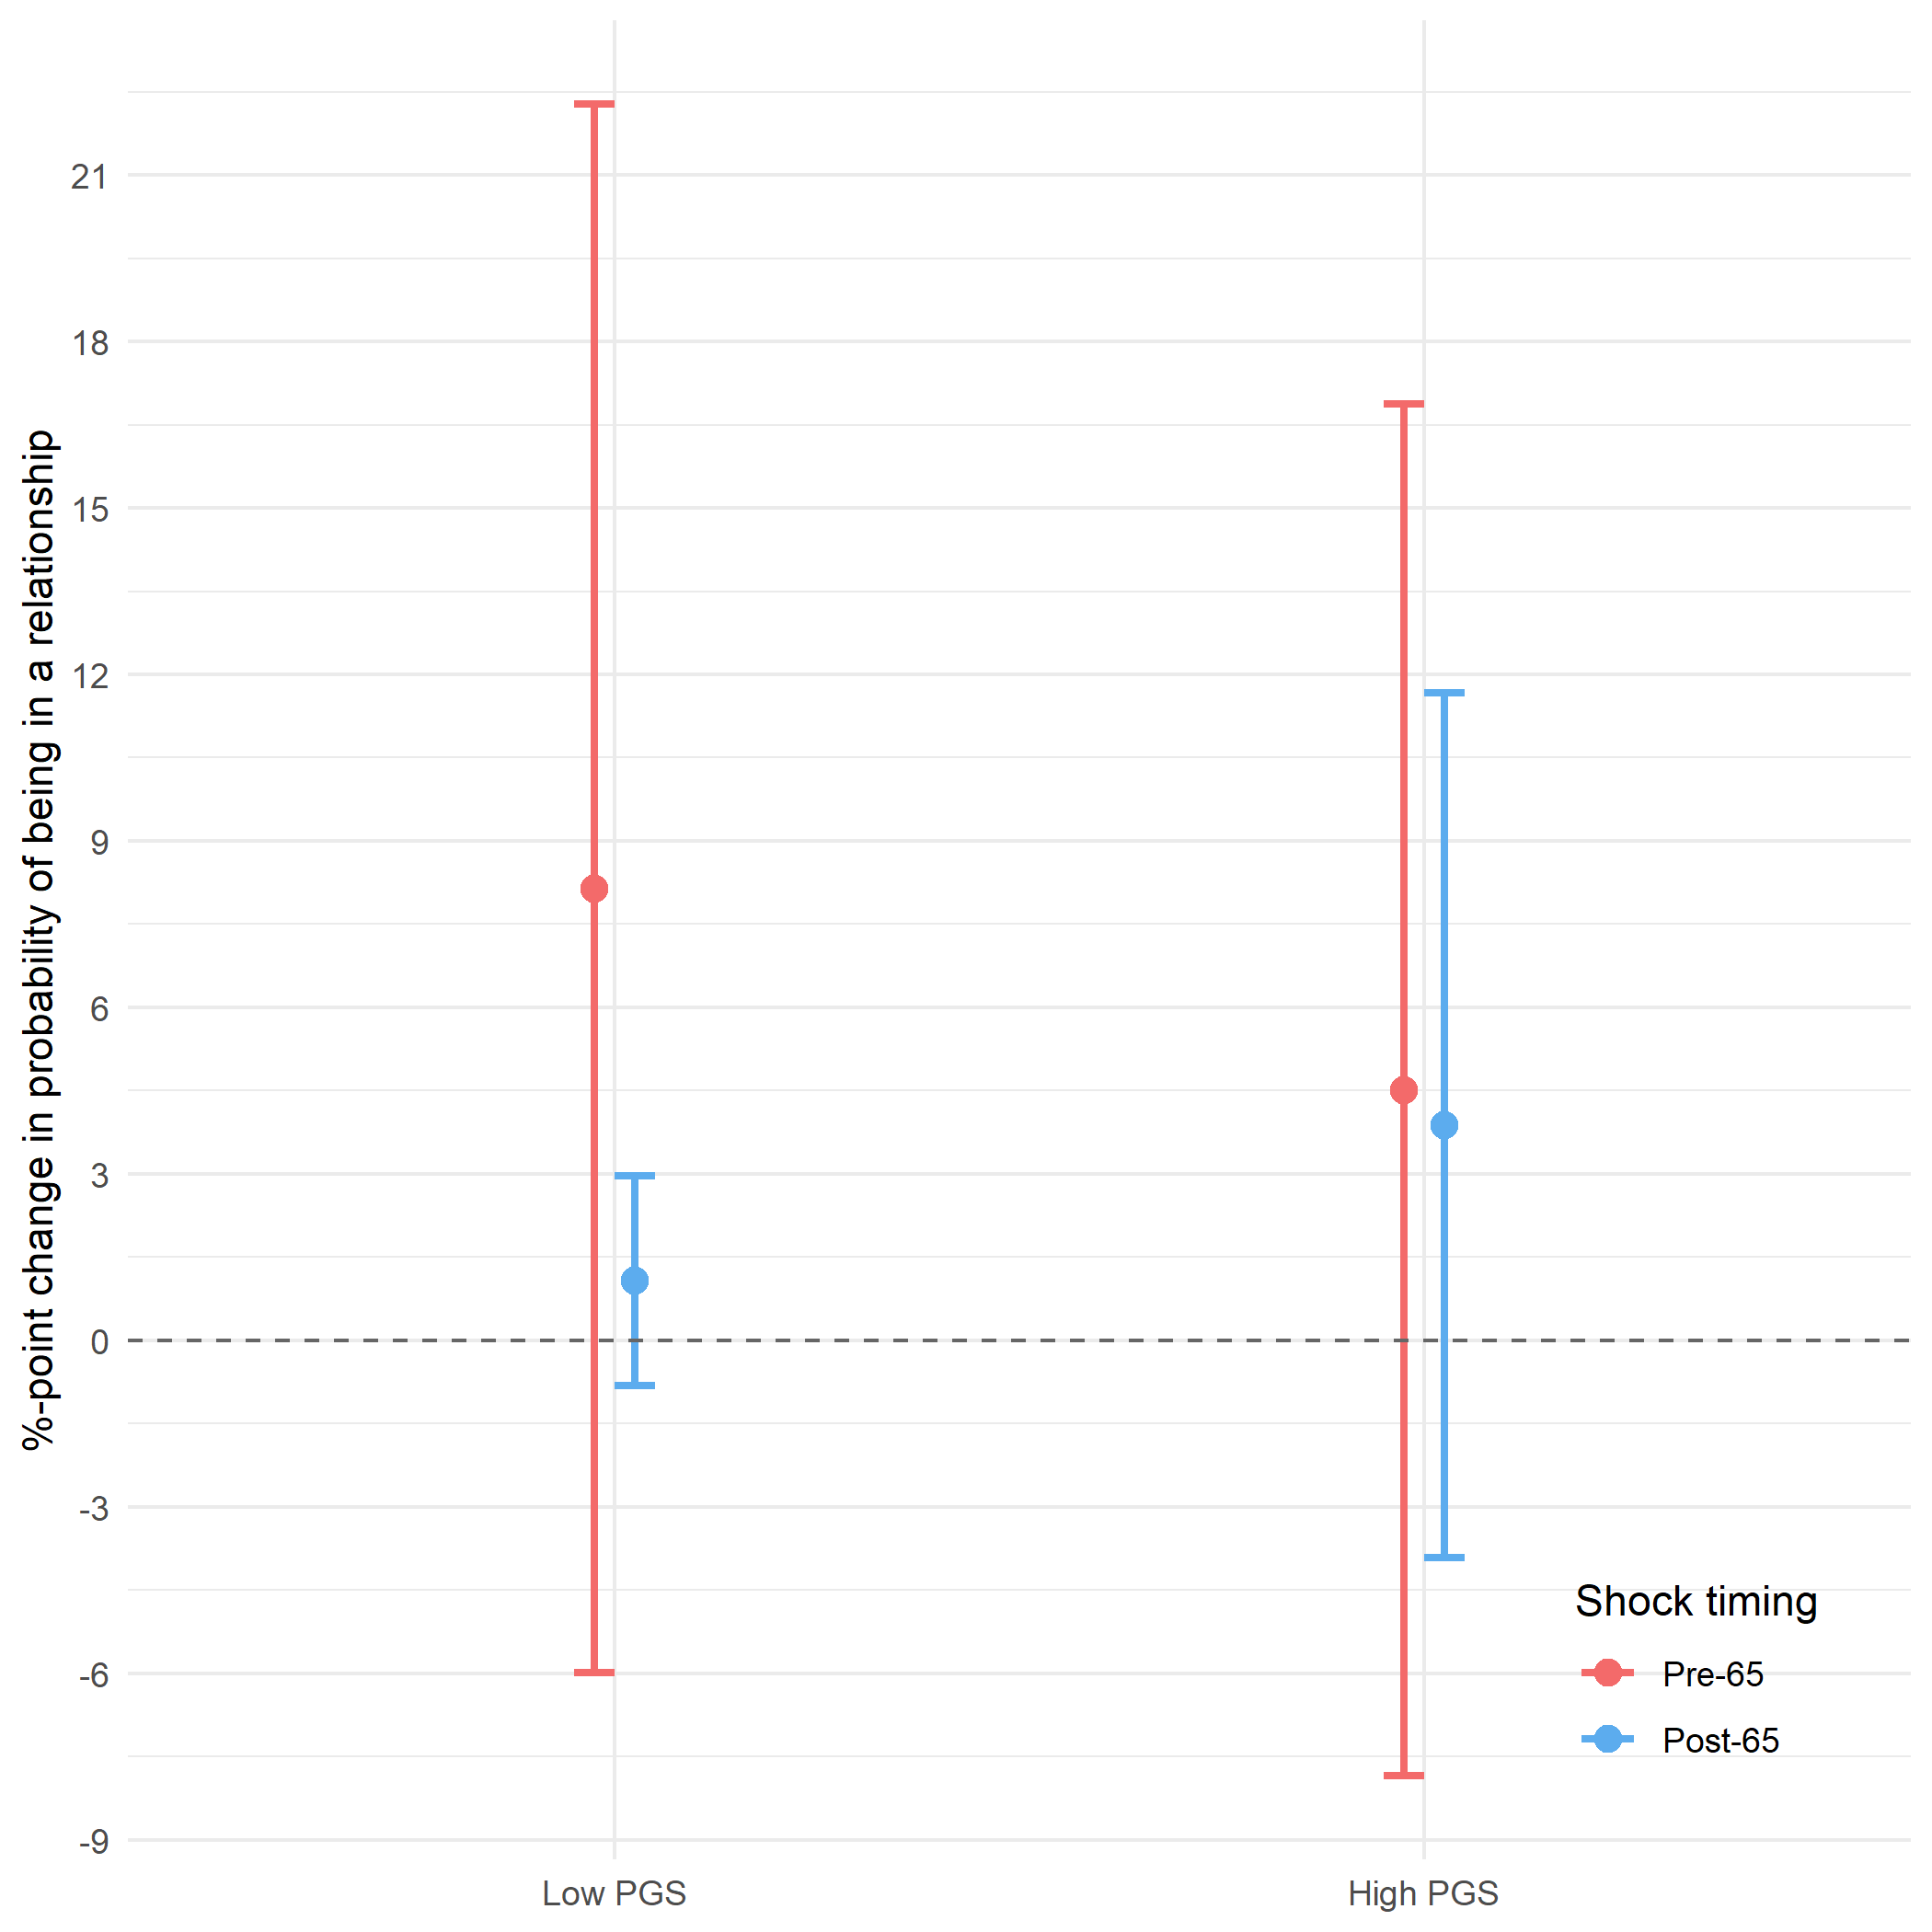
\includegraphics[height=0.8\textheight]{../../3_output/shock_effects/mpart_6070_100_cv.png}
\label{fig:mpart}
\end{figure}
%\hyperlink{frame:robustness}{\beamergotobutton{back}}
\end{frame}

%--------------------------------------------------------------% mpart
\begin{frame}
\frametitle{Partner smoking: not likely a Confounder}
Coefficient plot of the effect of the shock on having a partner.
\begin{figure}[hbtp]

\centering
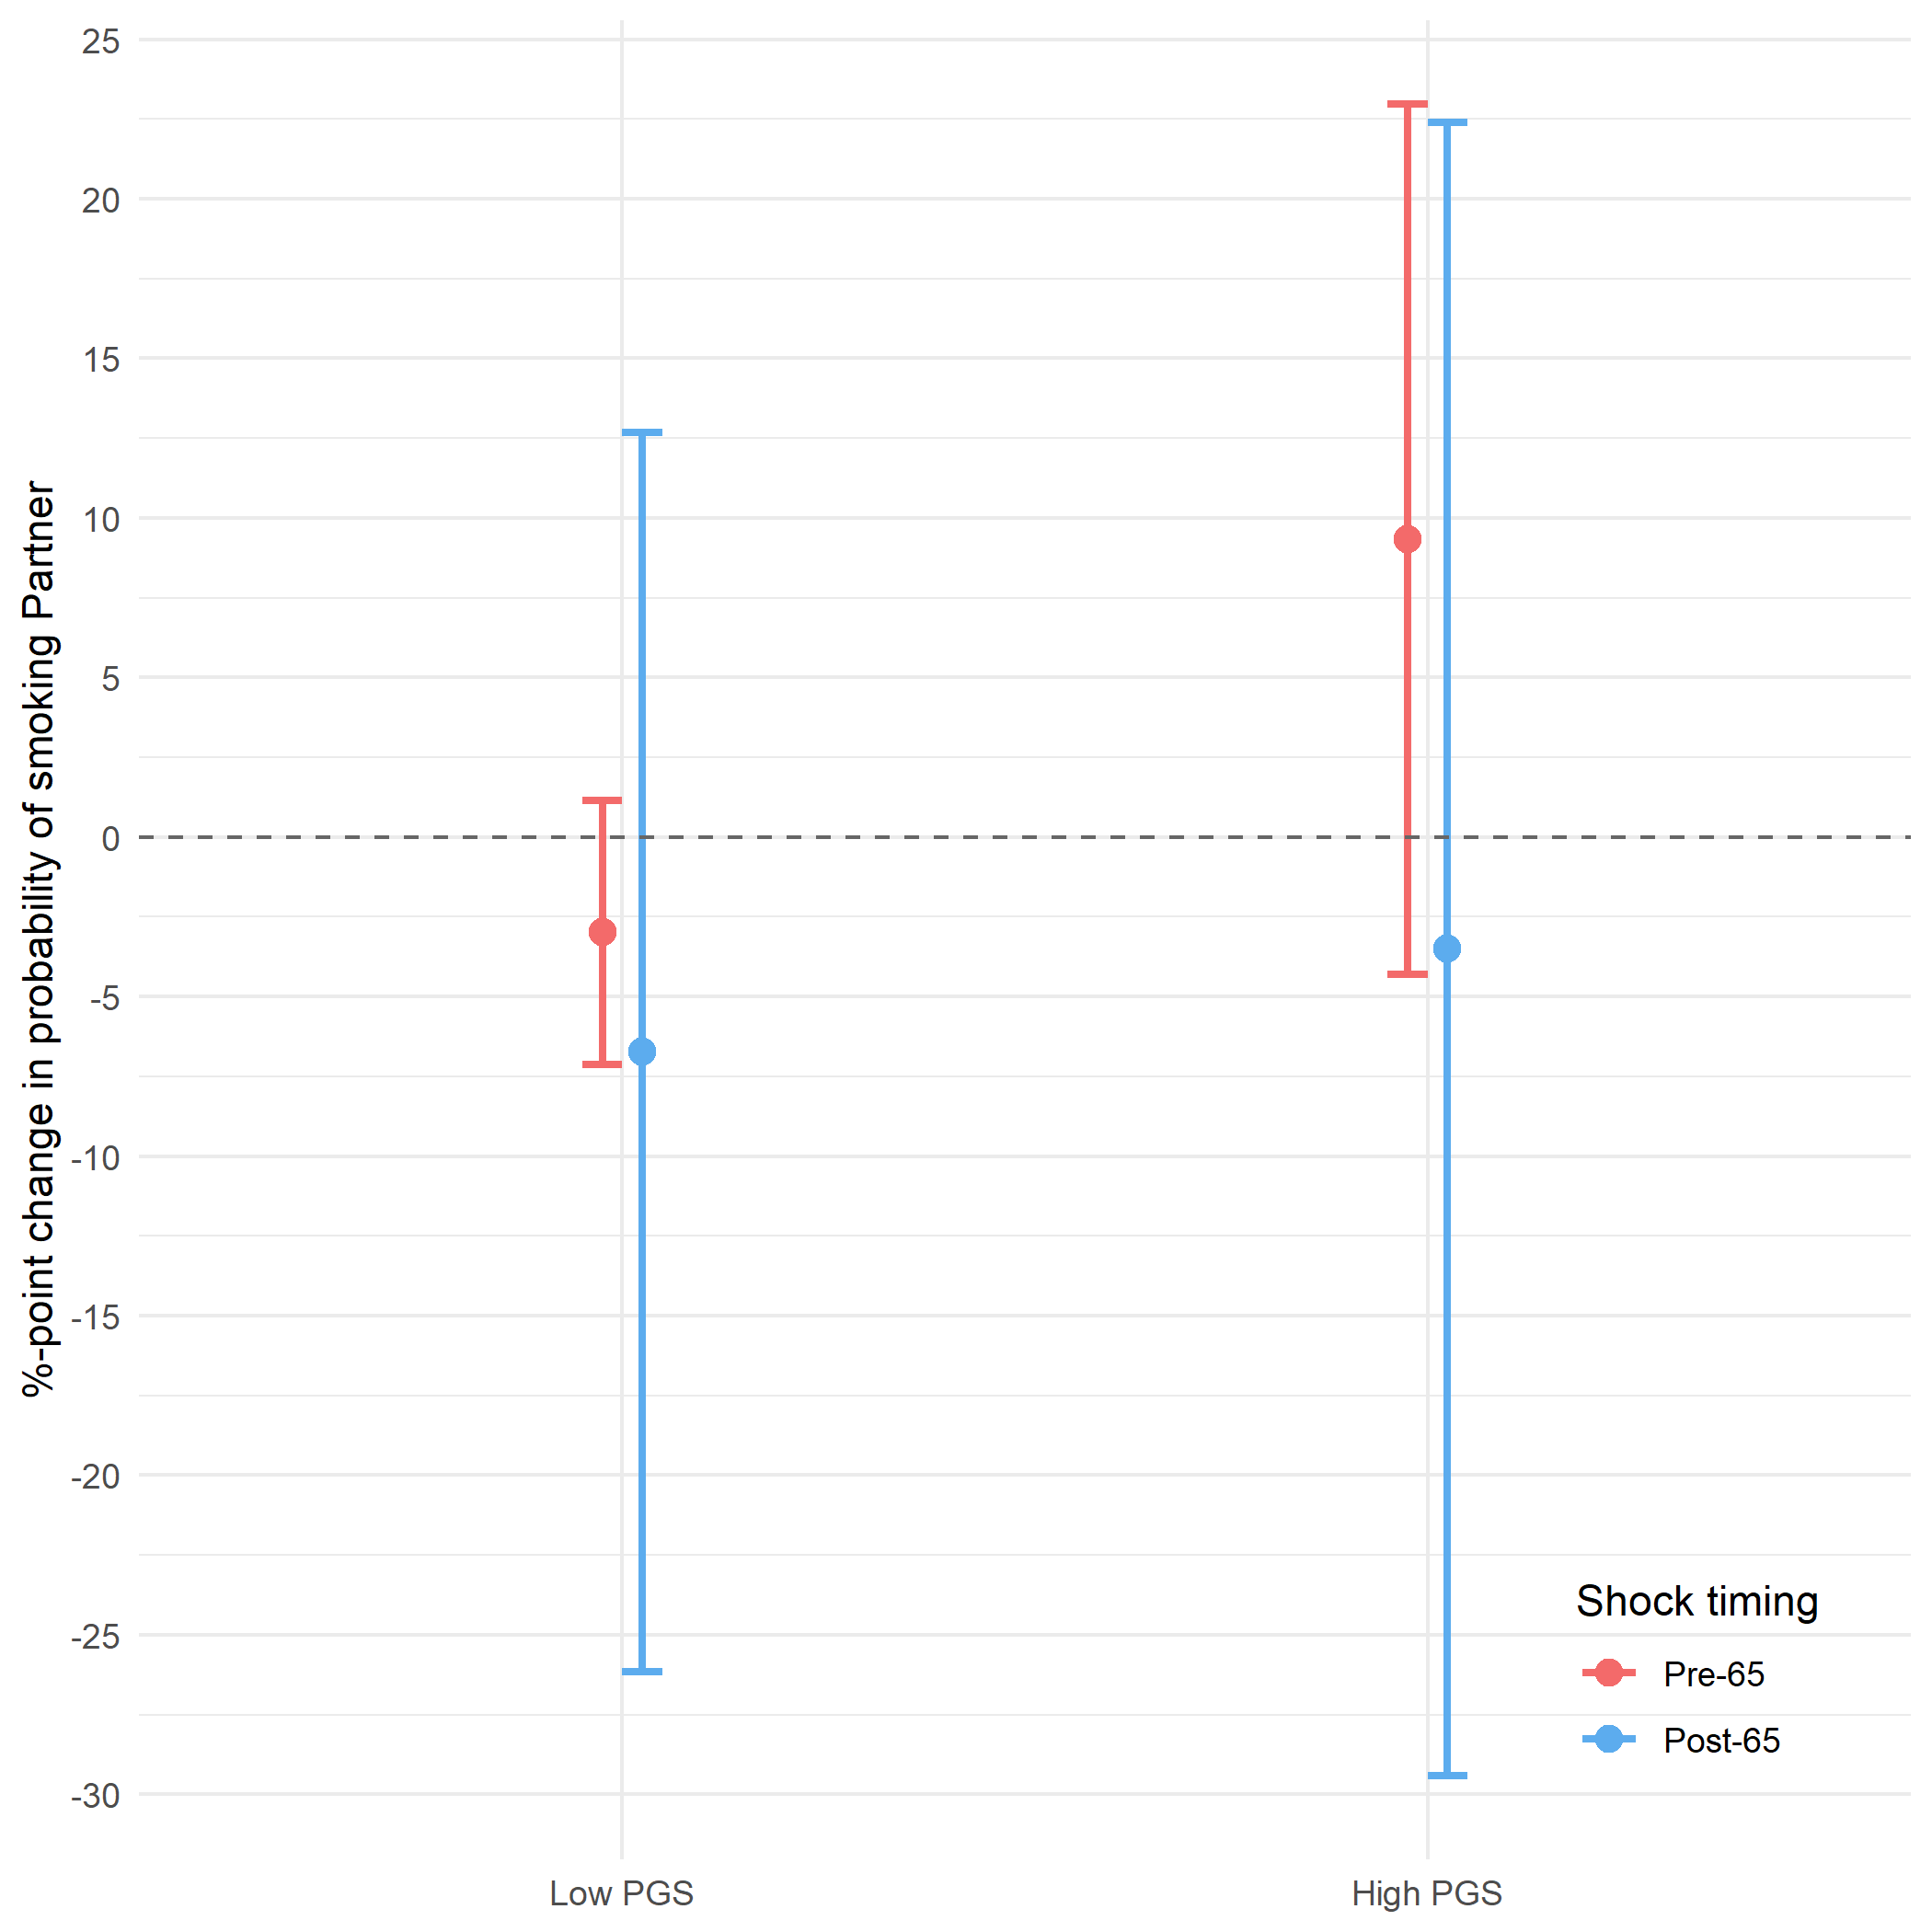
\includegraphics[height=0.8\textheight]{../../3_output/shock_effects/smokePartner_6070_100_cv.png}
\label{fig:smokePartner}
\end{figure}
%\hyperlink{frame:robustness}{\beamergotobutton{back}}
\end{frame}

%--------------------------------------------------------------% dead2
\begin{frame}
\frametitle{2 year mortality: not likely a Confounder}
Coefficient plot of the probability of dying within 2 years of the shock.
\begin{figure}[hbtp]
\centering
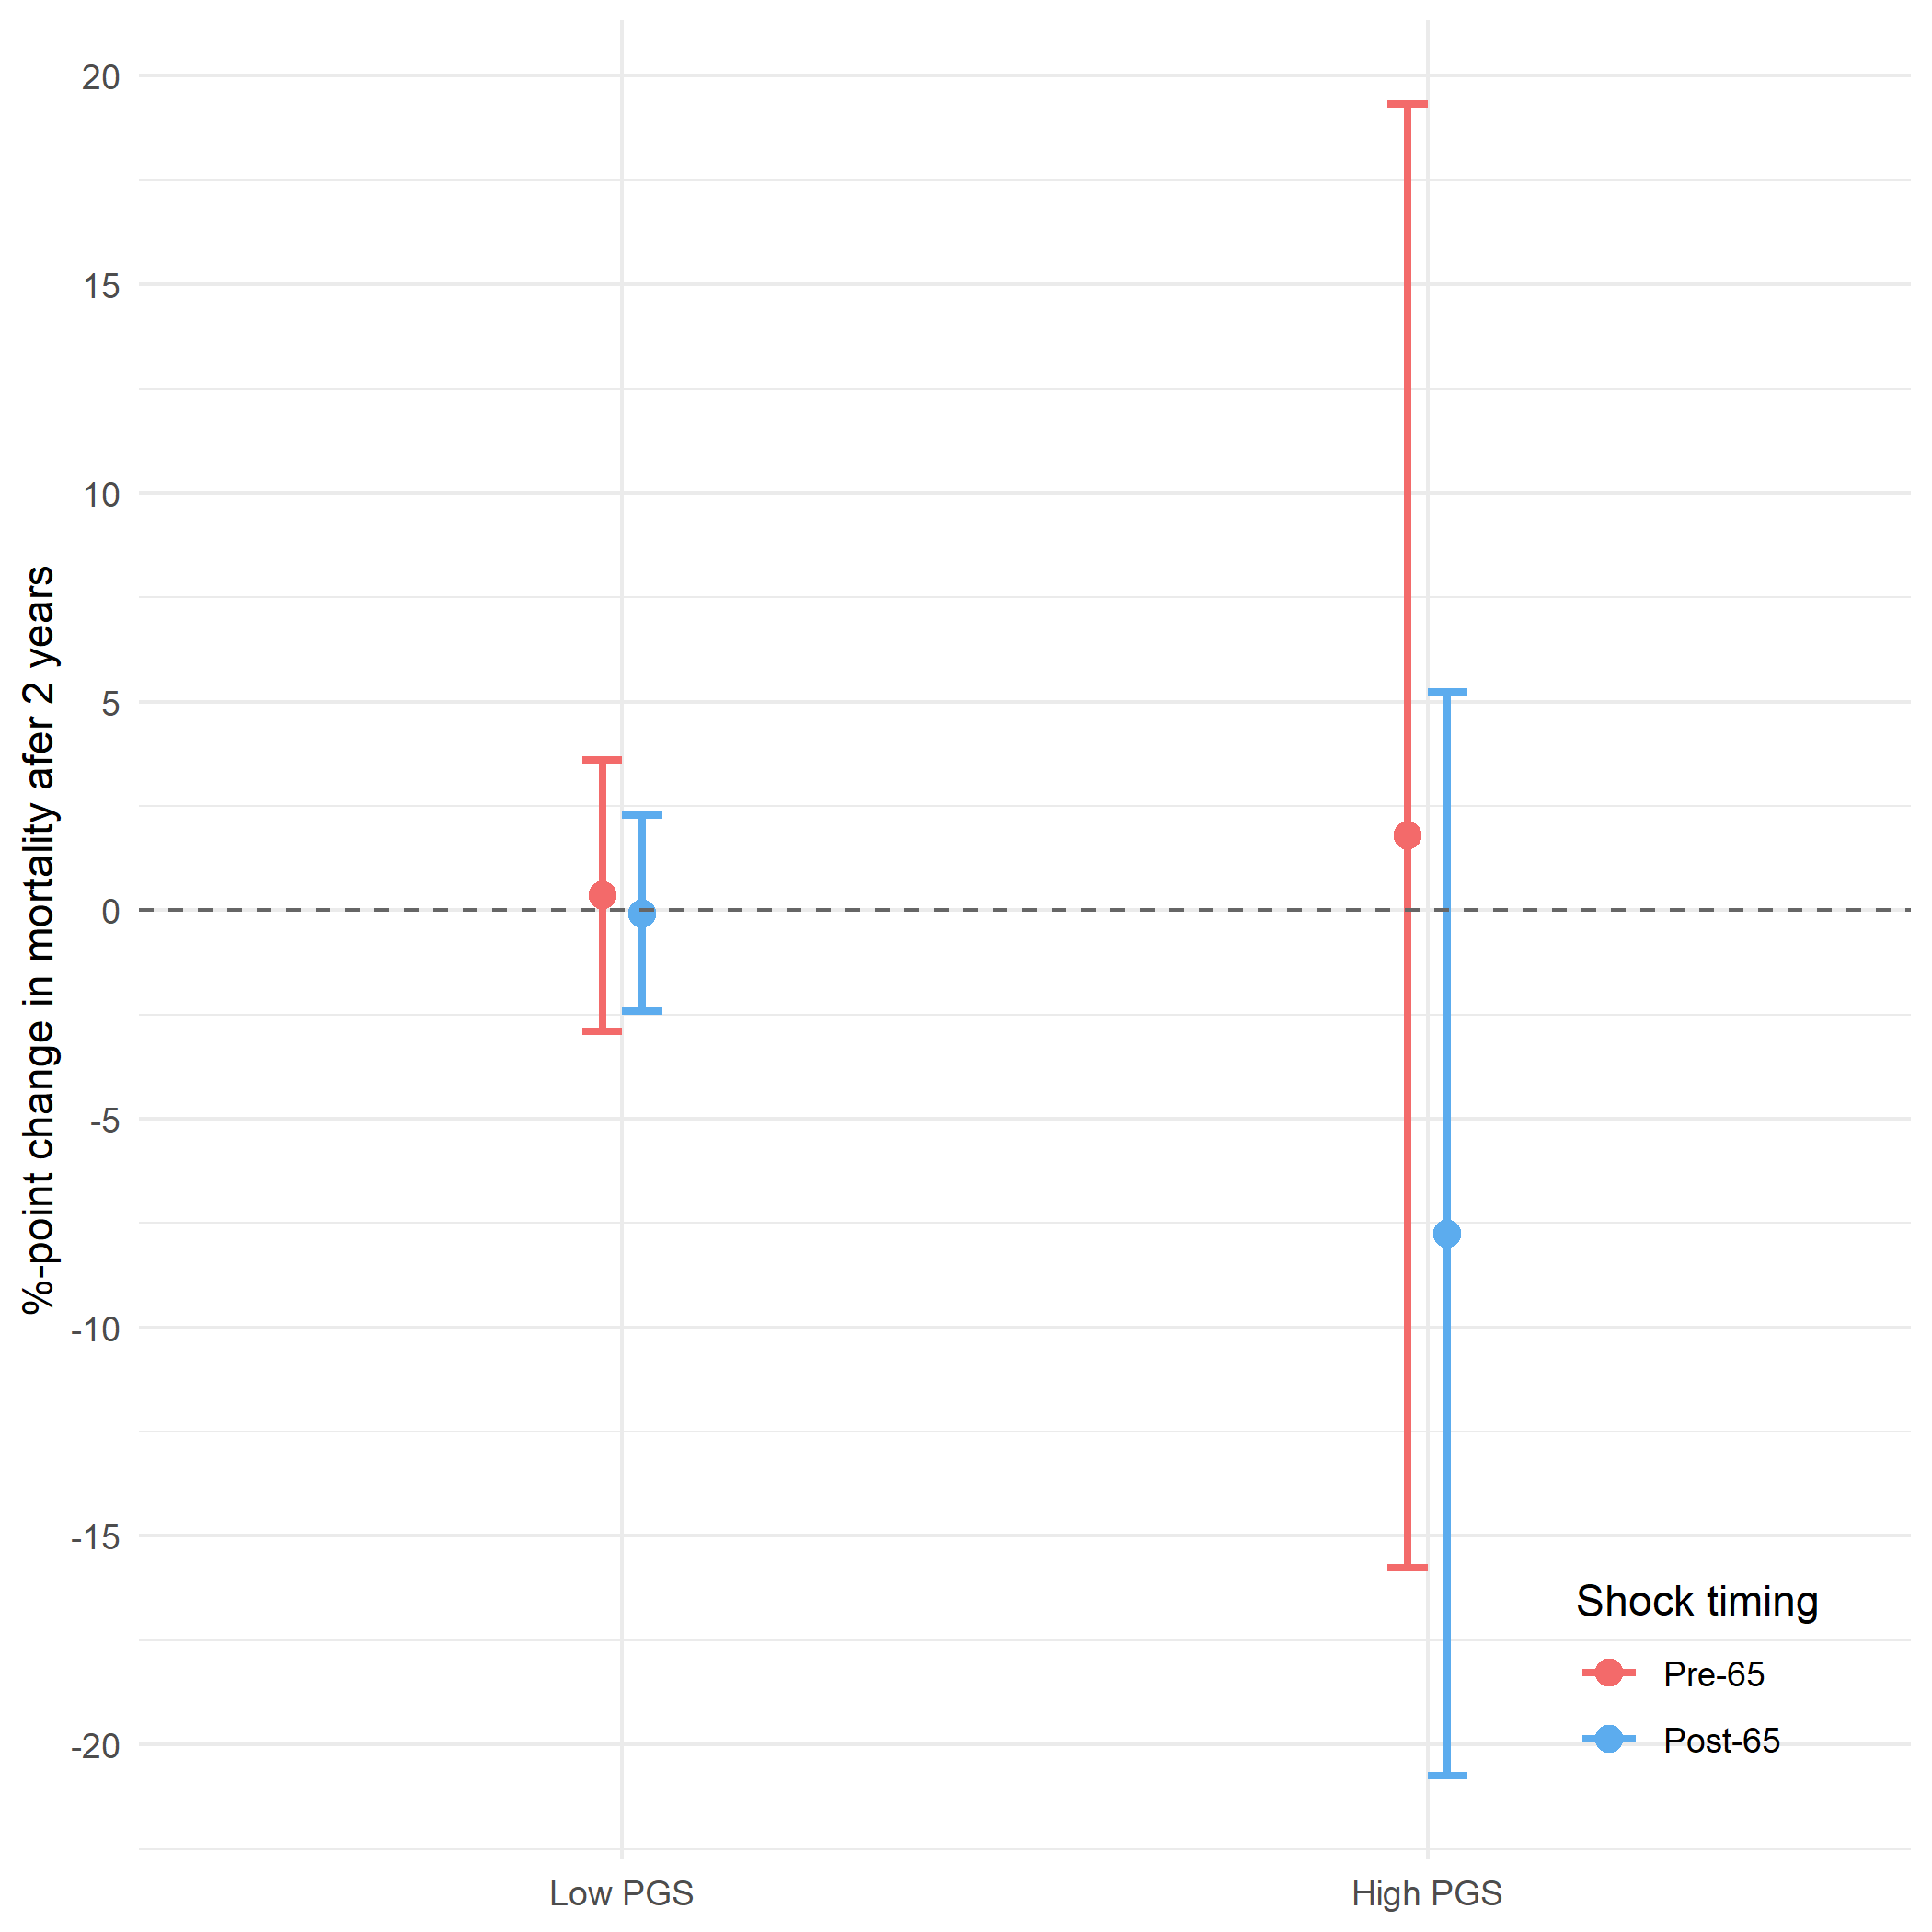
\includegraphics[height=0.8\textheight]{../../3_output/shock_effects/dead2_6070_100_cv.png}
\label{fig:dead2}
\end{figure}
%\hyperlink{frame:robustness}{\beamergotobutton{back}}
\end{frame}

%--------------------------------------------------------------% dead5
\begin{frame}
\frametitle{5 year mortality: not likely a Confounder}
Coefficient plot of the probability of dying within 5 years of the shock.
\begin{figure}[hbtp]
\centering
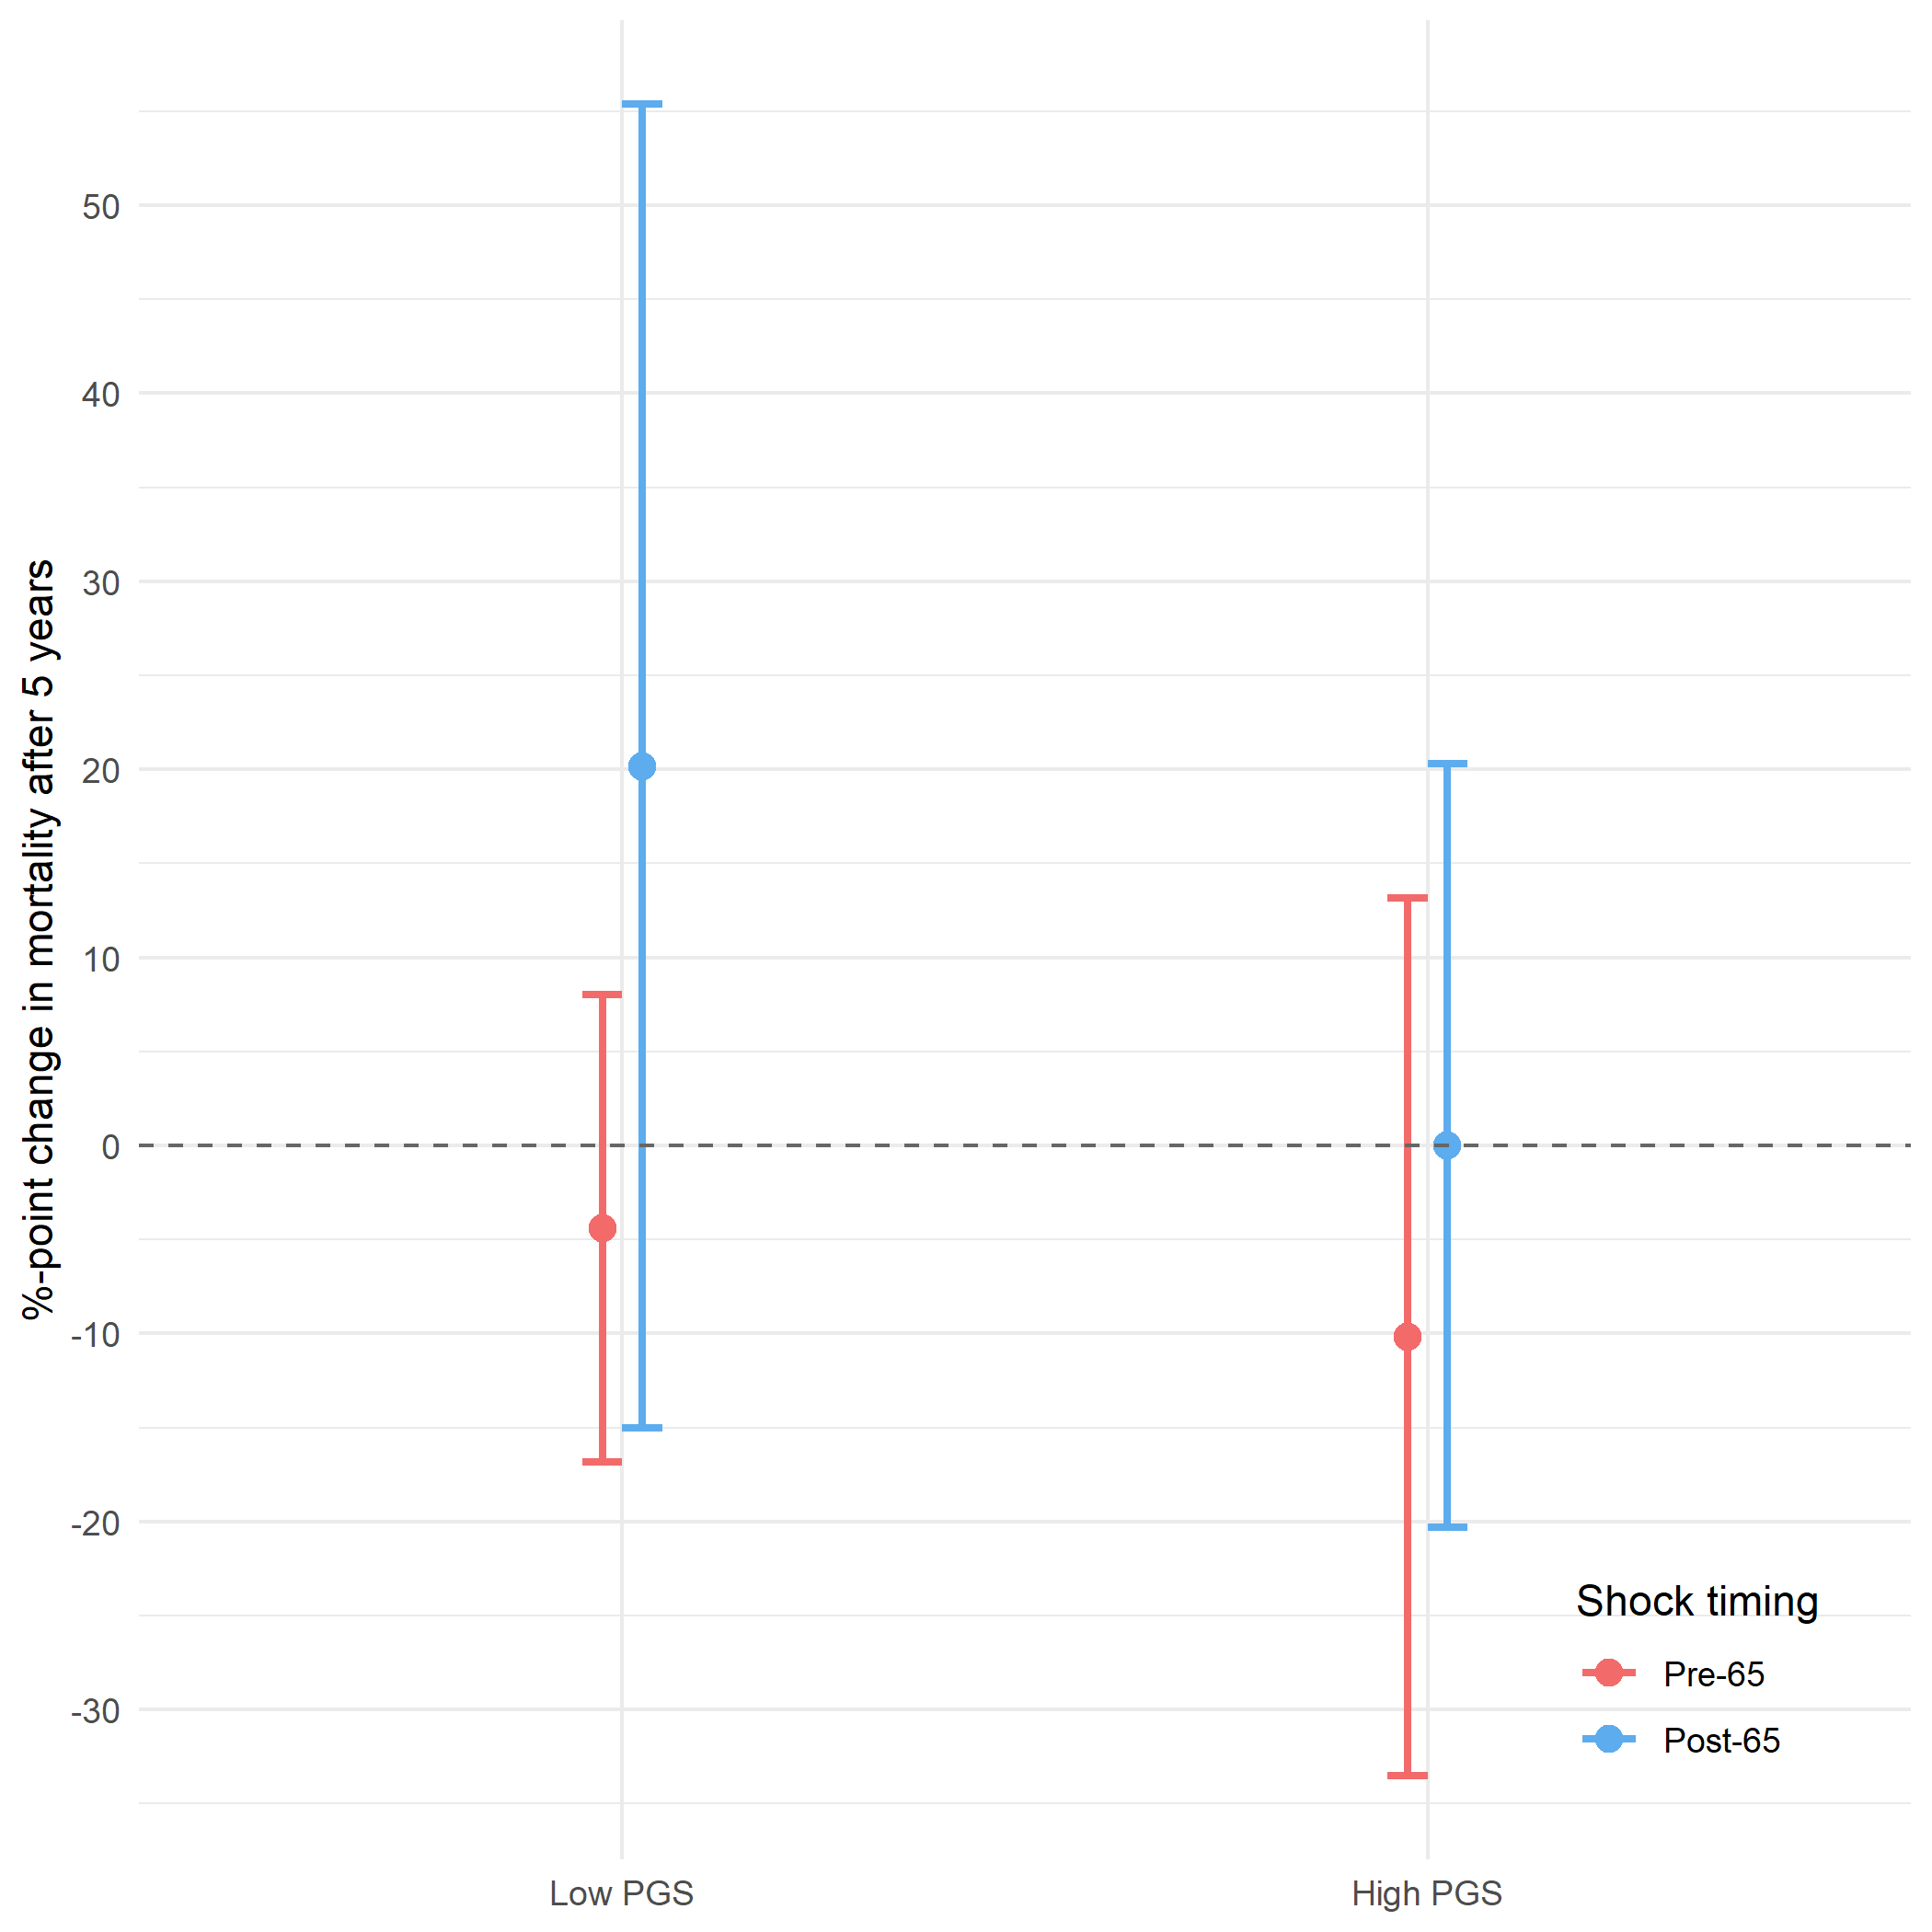
\includegraphics[height=0.8\textheight]{../../3_output/shock_effects/dead5_6070_100_cv.png}
\label{fig:dead5}
\end{figure}
%\hyperlink{frame:robustness}{\beamergotobutton{back}}
\end{frame}





%--------------------------------------------------------------%
\subsection{Robustness}
%--------------------------------------------------------------%
\begin{frame}
\frametitle{Robustness checks}
\label{frame:robustness}

Robustness checks:

\begin{itemize}
	\item Different cutoffs for high-PGS \hyperlink{fig:coeffplot25highPGS}{\beamergotobutton{PGS}}
	\begin{itemize}
		\item Still holds for lower quartile, not for highest
		\item Using continuous PGS, G$\times$E effect = -0.13 (0.11)
	\end{itemize}

	\vspace{1ex}

	\item Using the publicly available PGS (older GWAS from \cite{TAG2010}) \hyperlink{fig:oldPGS}{\beamergotobutton{PGS}}
	\begin{itemize}
		\item Similar pattern
	\end{itemize}

	\vspace{1ex}

	\item Different cutoffs for uninsured \hyperlink{fig:coeffplot66unins}{\beamergotobutton{uninsured}}
	\begin{itemize}
		\item Noisy results for uninsured only 1/3 of the times
	\end{itemize}

	\vspace{1ex}

	\item Different cutoffs for age \hyperlink{fig:coeffplot59-71}{\beamergotobutton{age}}
	\begin{itemize}
		\item Noisy results after age 72
	\end{itemize}
\end{itemize}

\end{frame}

%--------------------------------------------------------------%
\begin{frame}
\frametitle{Robustness: high PGS if above 25$^{th}$ percentile}
Coefficient plot of the main regression.
\begin{figure}[hbtp]

\centering
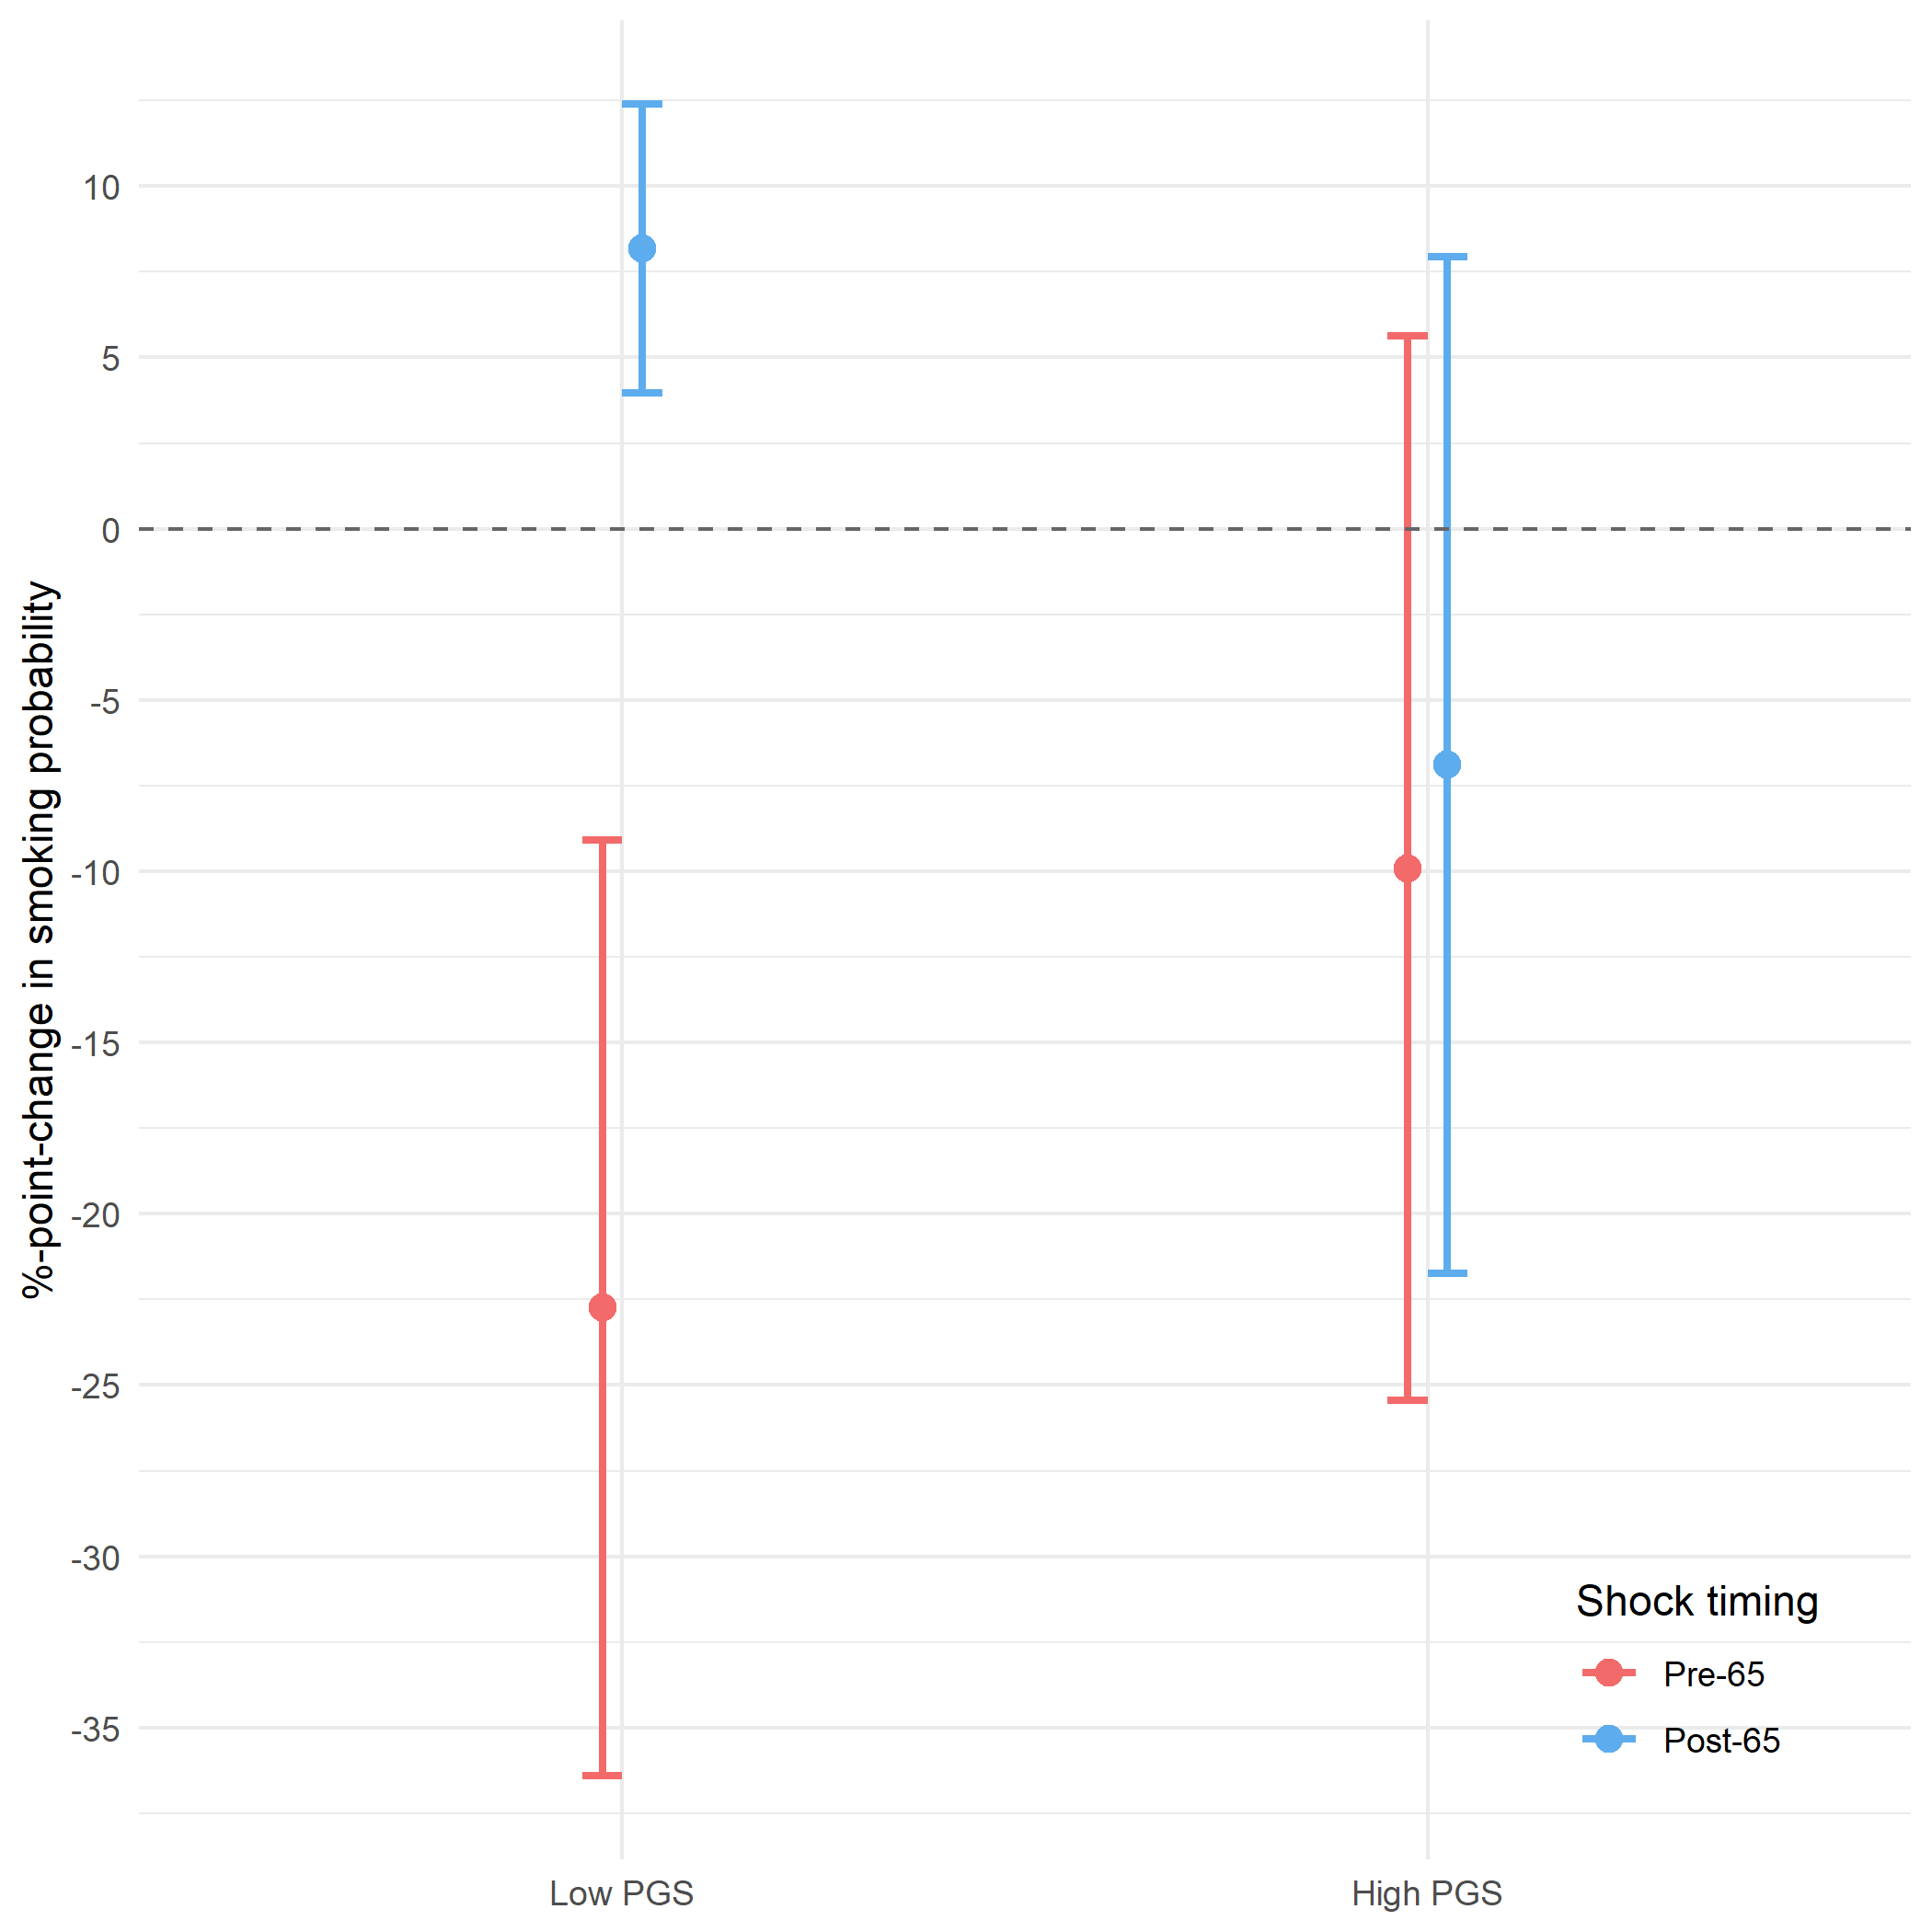
\includegraphics[height=0.8\textheight]{../../3_output/shock_effects/robustness_6070_25pt_cv.png}
\label{fig:coeffplot25highPGS}
\end{figure}
\hyperlink{frame:robustness}{\beamergotobutton{back}}
\end{frame}

%--------------------------------------------------------------%
\begin{frame}
\frametitle{Robustness: high PGS if above 50$^{th}$ percentile}
Coefficient plot of the main regression.
\begin{figure}[hbtp]

\centering
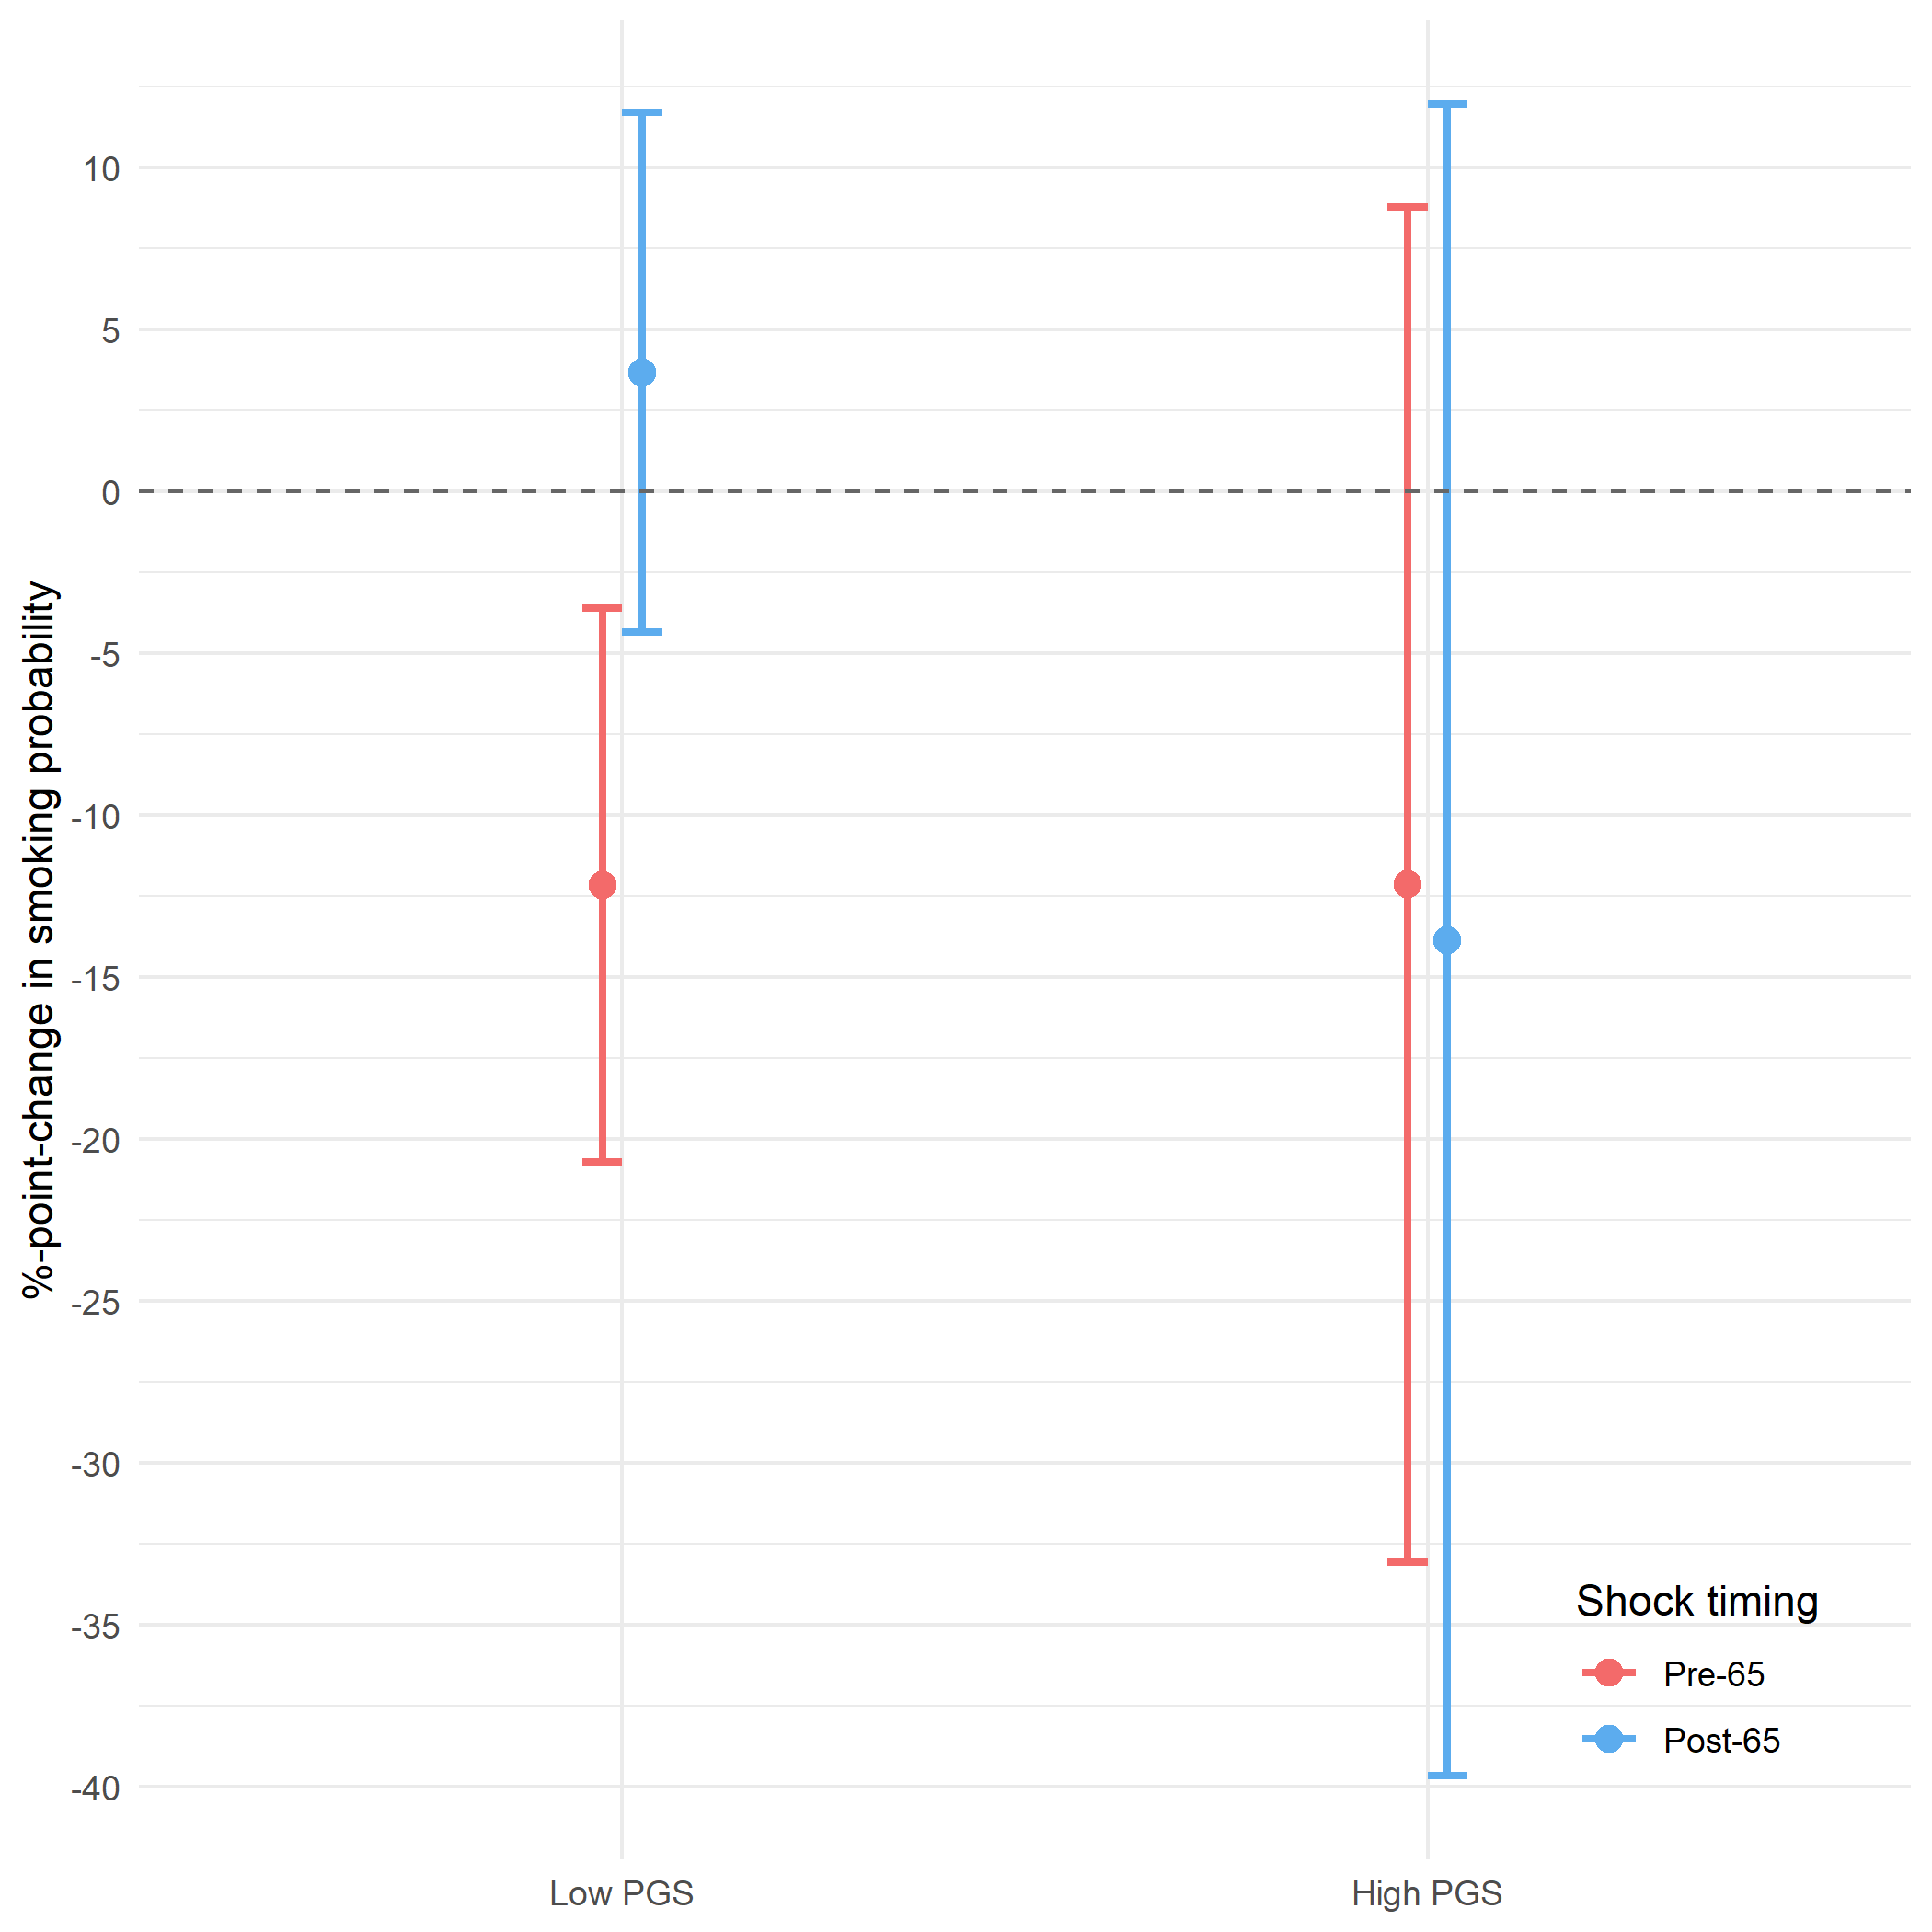
\includegraphics[height=0.8\textheight]{../../3_output/shock_effects/robustness_6070_50pt_cv.png}
\label{fig:coeffplot50highPGS}
\end{figure}
\hyperlink{frame:robustness}{\beamergotobutton{back}}
\end{frame}

%--------------------------------------------------------------%
\begin{frame}
\frametitle{Robustness: high PGS if above 75$^{th}$ percentile}
Coefficient plot of the main regression.
\begin{figure}[hbtp]

\centering
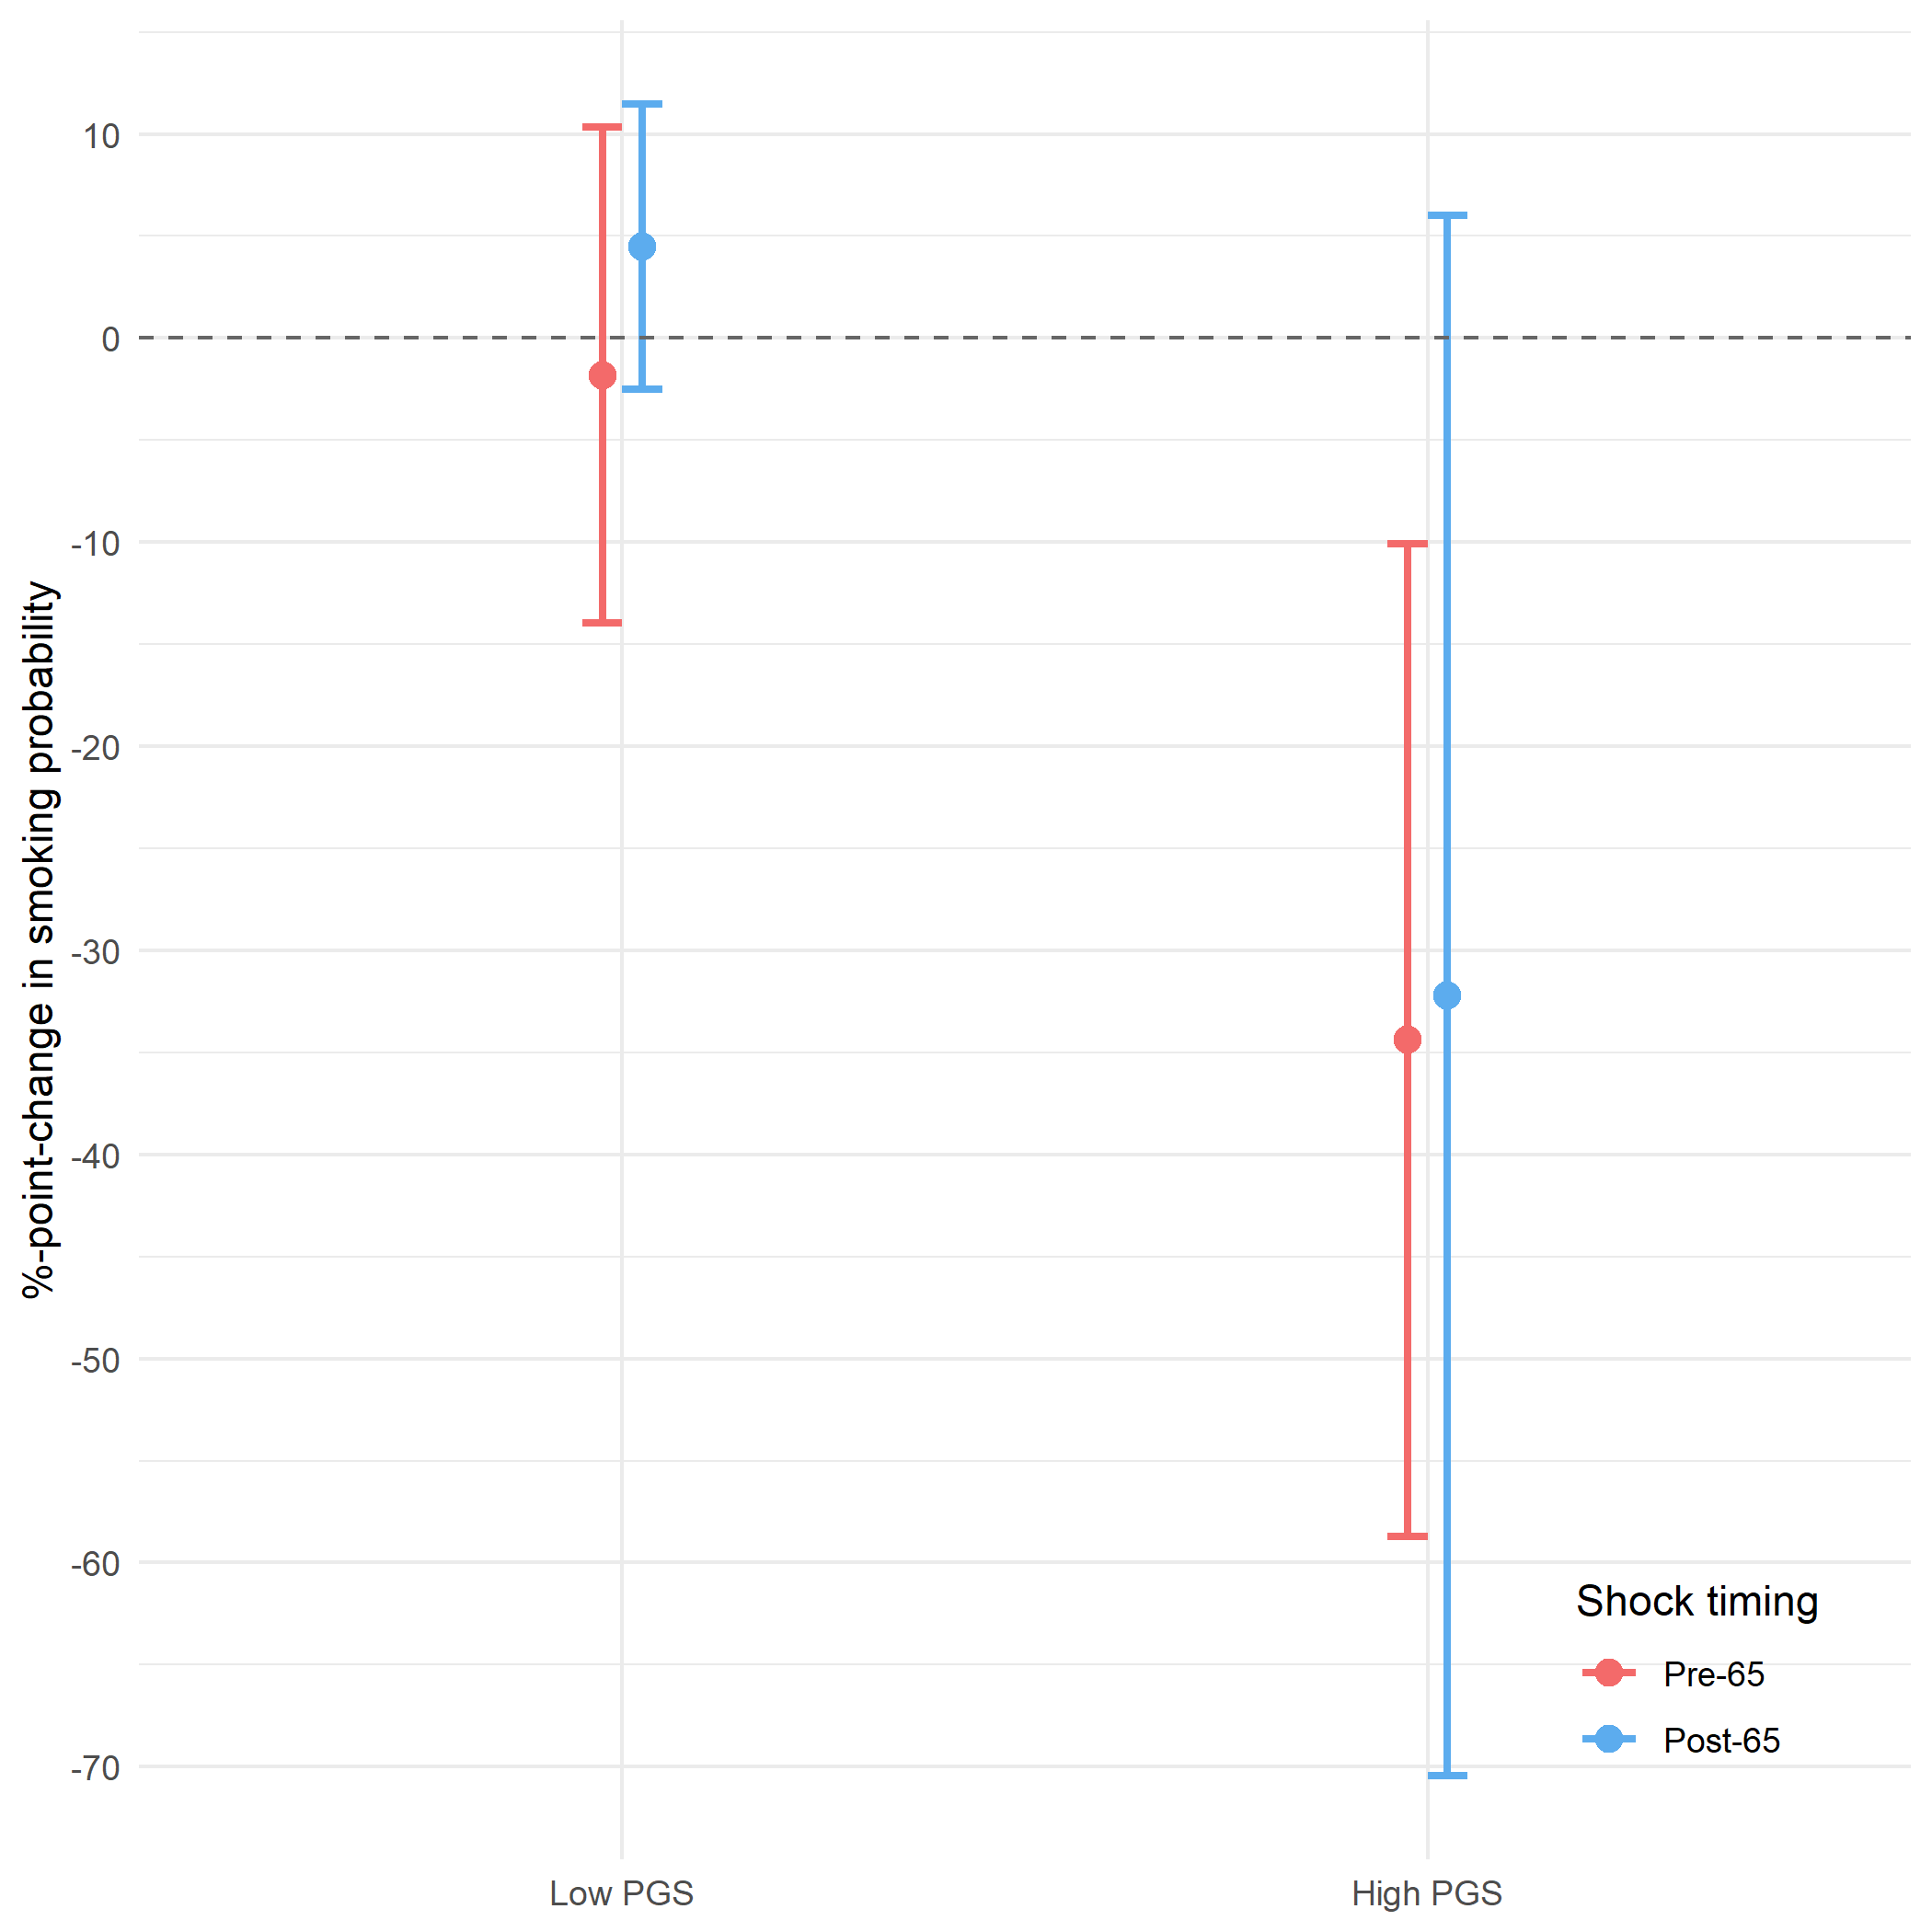
\includegraphics[height=0.8\textheight]{../../3_output/shock_effects/robustness_6070_75pt_cv.png}
\label{fig:coeffplot75highPGS}
\end{figure}
\hyperlink{frame:robustness}{\beamergotobutton{back}}
\end{frame}

%--------------------------------------------------------------%
\begin{frame}
\frametitle{Robustness: using publicly available PGS (older GWAS)}
Coefficient plot of the main regression.
\begin{figure}[hbtp]

\centering
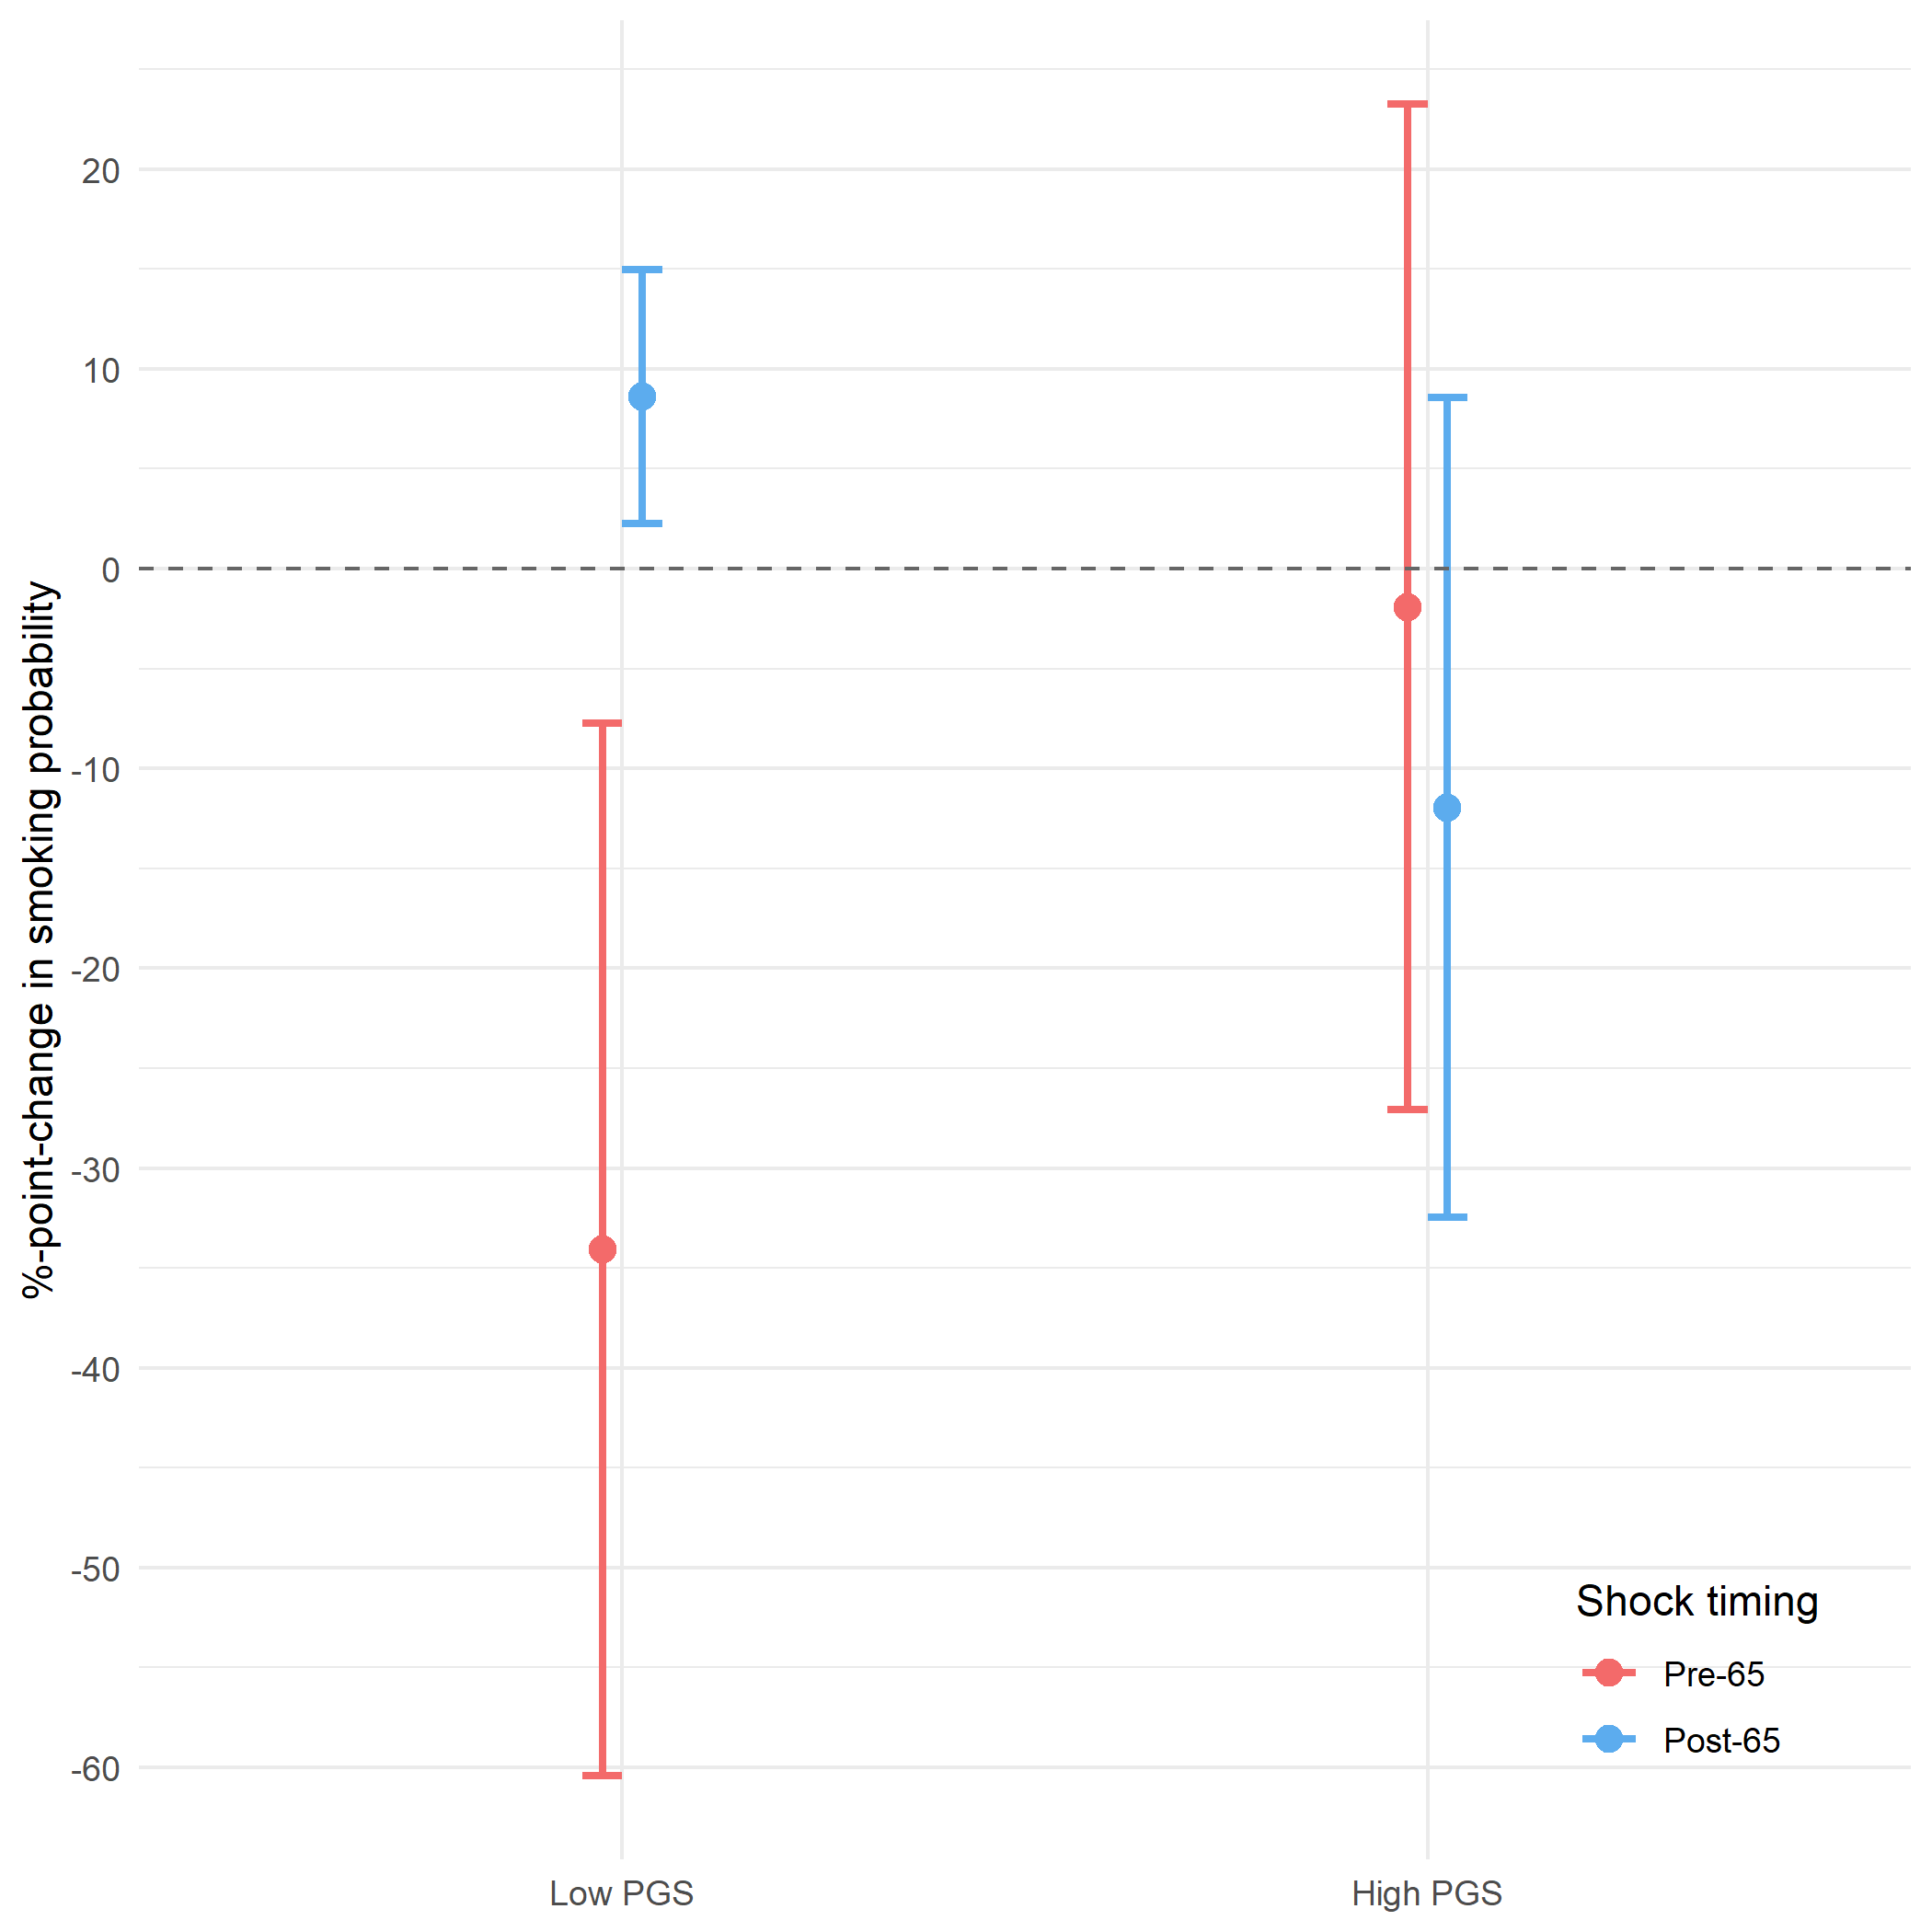
\includegraphics[height=0.8\textheight]{../../3_output/shock_effects/robustness_6070_oldpgs_cv.png}

\label{fig:oldPGS}
\end{figure}
\hyperlink{frame:robustness}{\beamergotobutton{back}}
\end{frame}


%--------------------------------------------------------------%
\subsection[Split]{Is it really genes?}
%--------------------------------------------------------------%
\begin{frame} \label{frame:otherX}
\frametitle{Is it really genes?}
Are there other characteristics that might be driving this relationship?

\begin{itemize}
	\item Try to cut the data according to other dimensions:
	\begin{itemize}
		\item Cognitive skills 	\hyperlink{fig:cog}{\beamergotobutton{}}
		\item Conscientiousness \hyperlink{fig:consc}{\beamergotobutton{}}
		\item Risk aversion 	\hyperlink{fig:risk}{\beamergotobutton{}}
		\item Gender 			\hyperlink{fig:gender}{\beamergotobutton{}}
		\item Education 		\hyperlink{fig:edu}{\beamergotobutton{}}
		\item Income 			\hyperlink{fig:income}{\beamergotobutton{}}
	\end{itemize}

	\item Or according to other PGS:
	\begin{itemize}
		\item Cognition PGS 	\hyperlink{fig:cogPGS}{\beamergotobutton{}}
		%\item Non-cognitive PGS \hyperlink{fig:noncogPGS}{\beamergotobutton{}}
		\item Risk aversion PGS	\hyperlink{fig:riskPGS}{\beamergotobutton{}}
		%\item Education PGS		\hyperlink{fig:ea3PGS}{\beamergotobutton{}}
	\end{itemize}
\end{itemize}

\end{frame}

%--------------------------------------------------------------%
\begin{frame}
\frametitle{Split by cognitive ability}

\begin{figure}[hbtp]
\centering
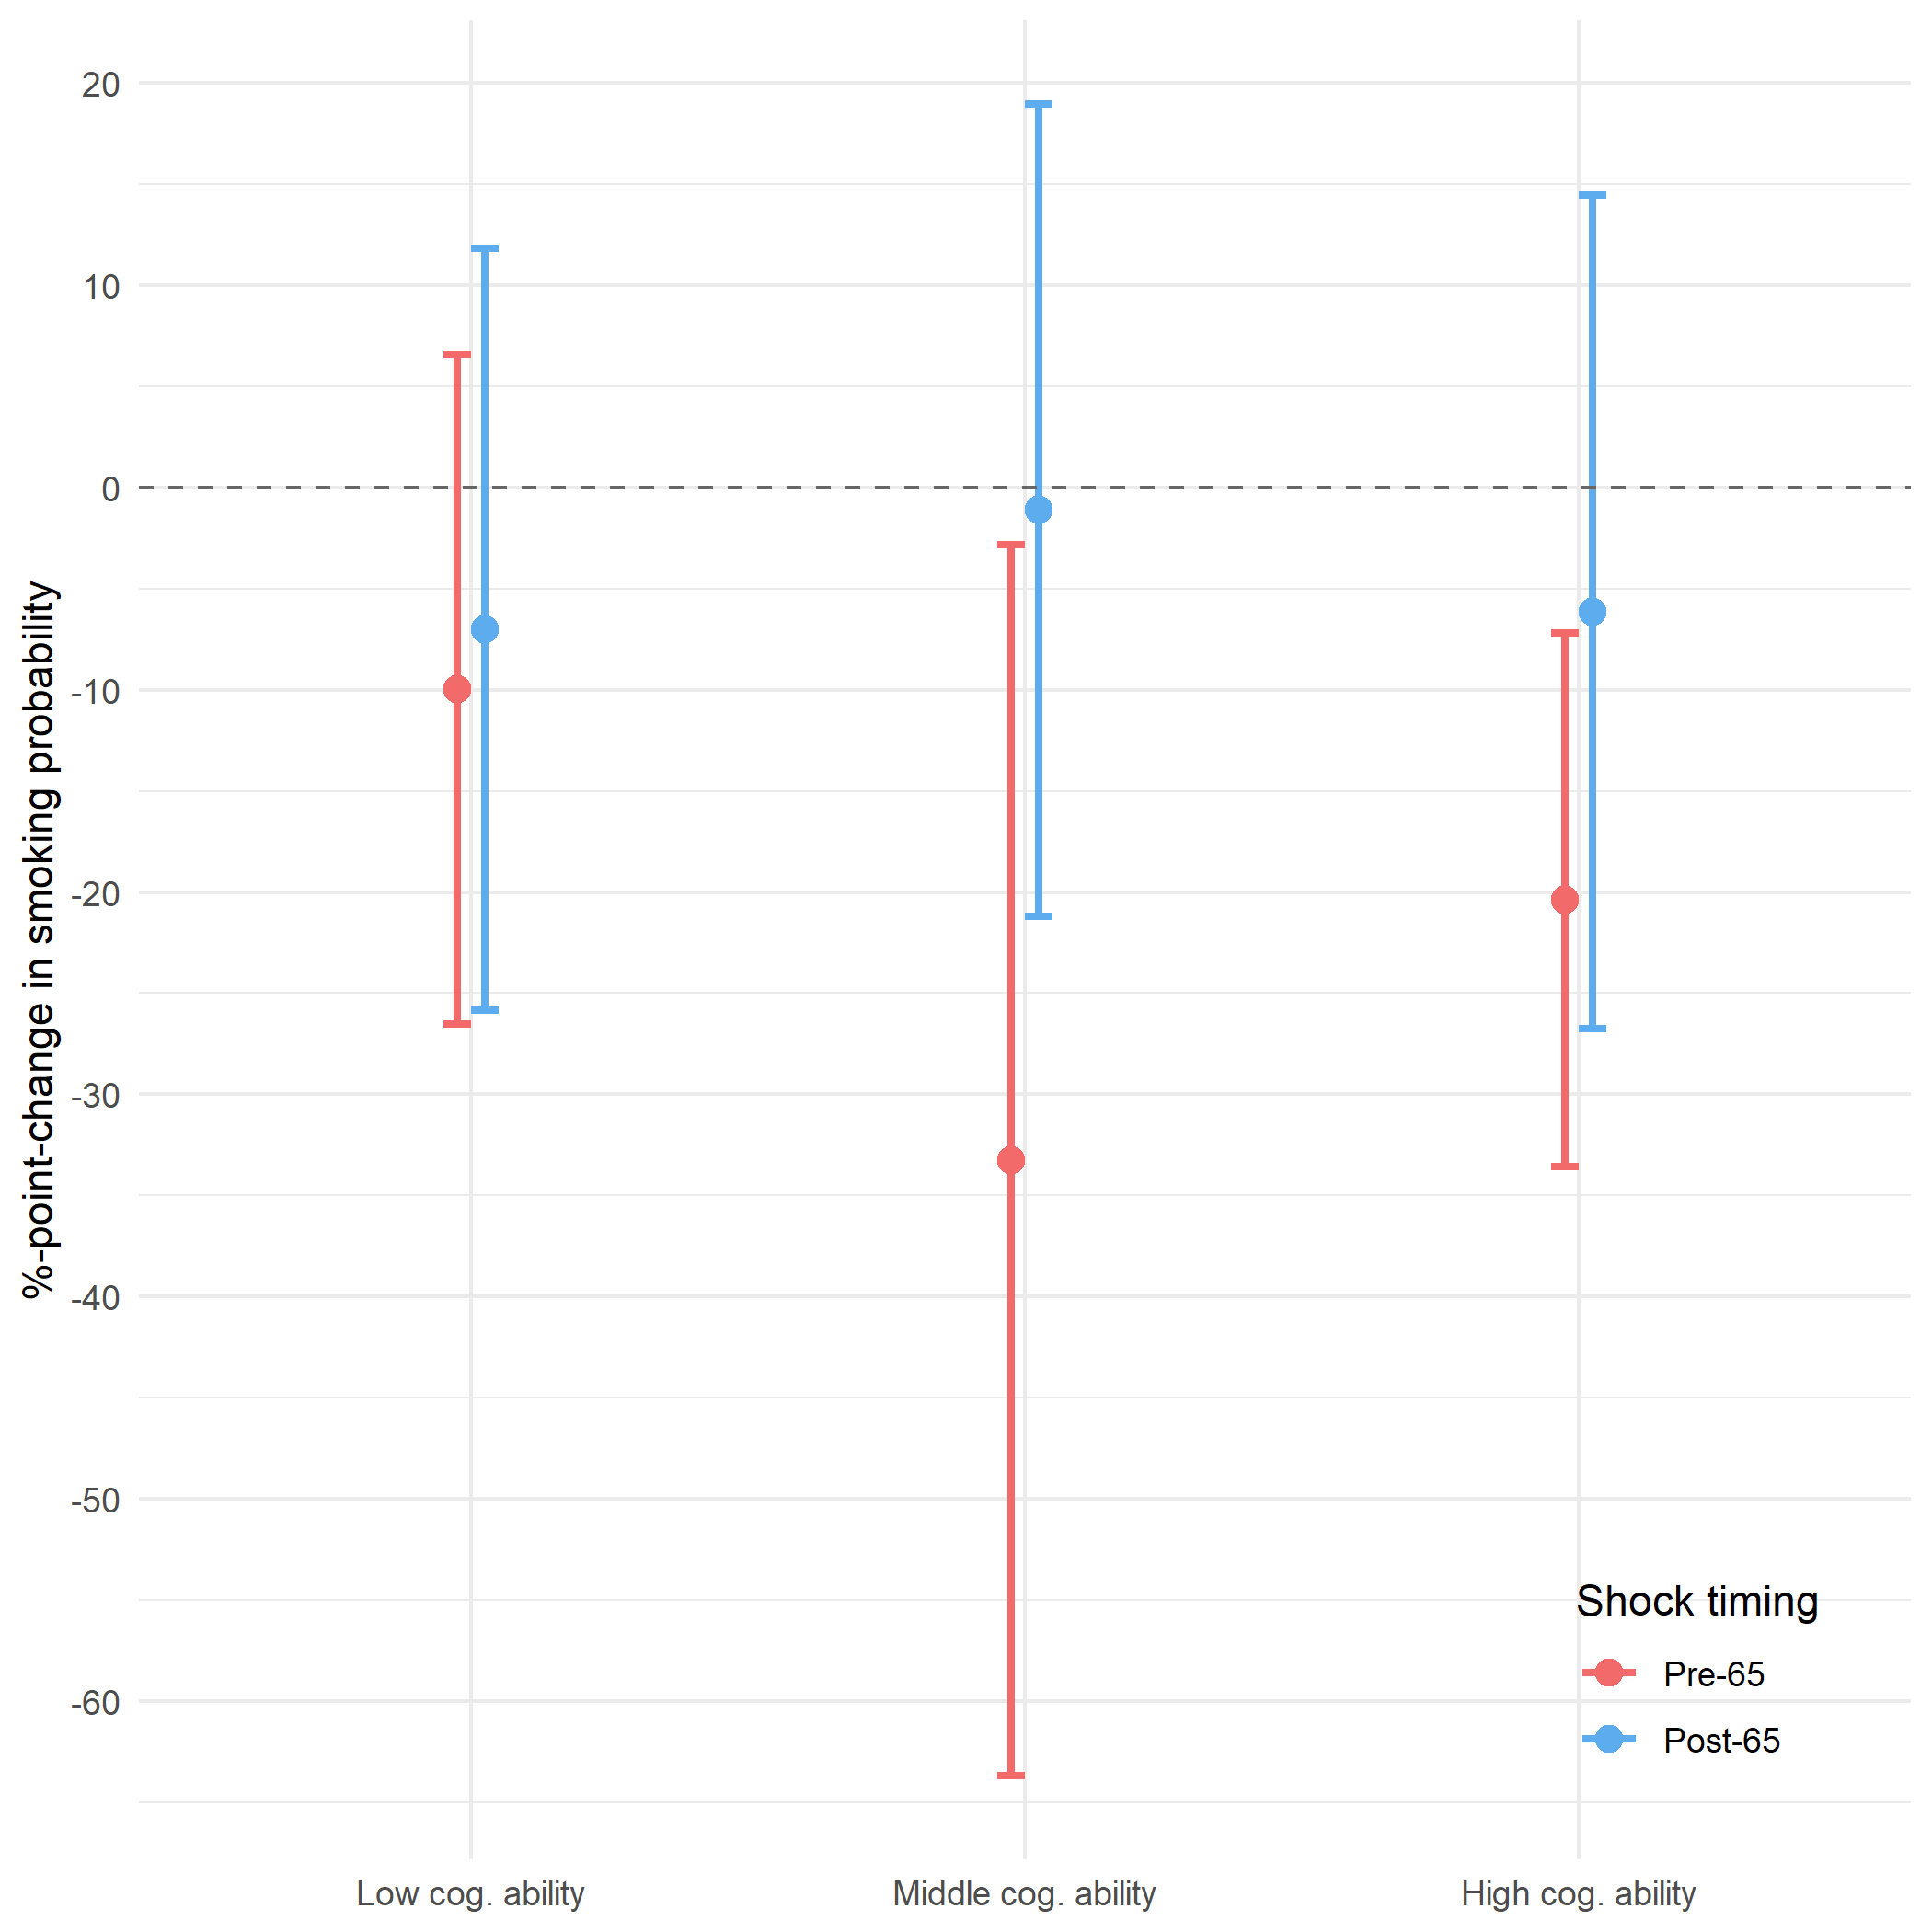
\includegraphics[height=0.8\textheight]{../../3_output/shock_effects/cog_6070_100_cv.png}
\label{fig:cog}
\end{figure}
\hyperlink{frame:otherX}{\beamergotobutton{back}}
\end{frame}

%--------------------------------------------------------------%
\begin{frame}
\frametitle{Split by conscientiousness}

\begin{figure}[hbtp]
\centering
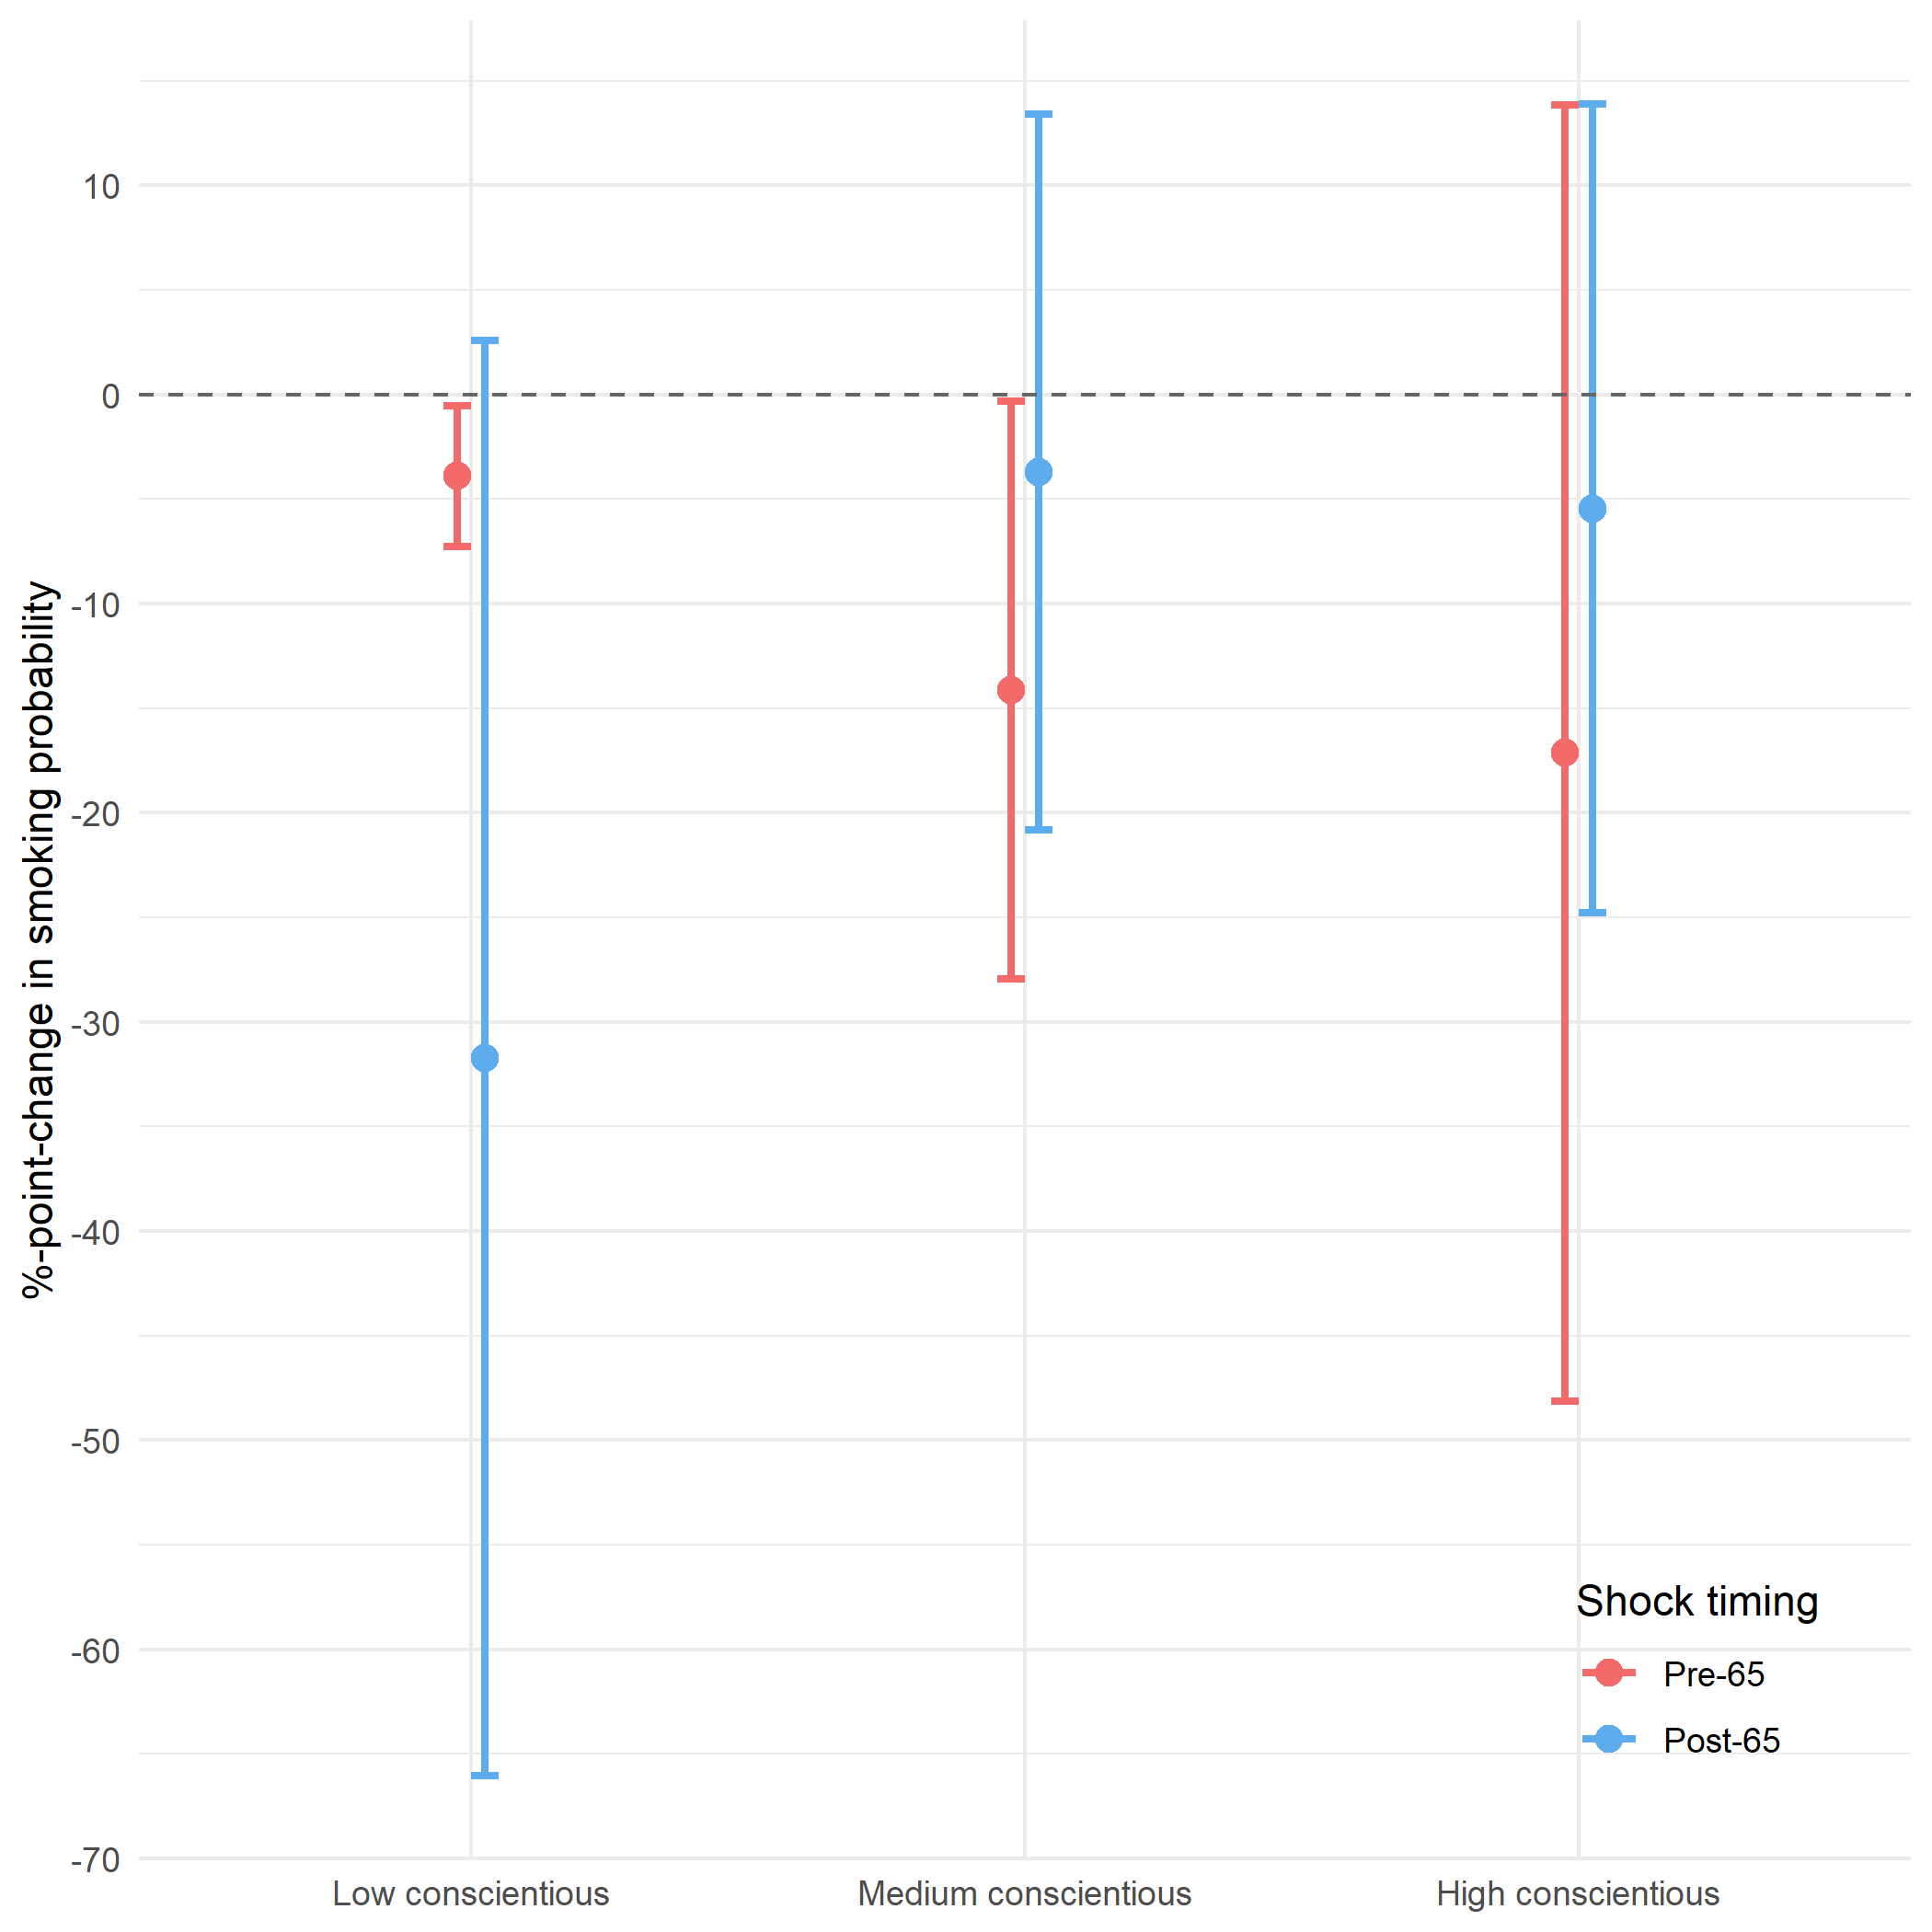
\includegraphics[height=0.8\textheight]{../../3_output/shock_effects/consc_6070_100_cv.png}
\label{fig:consc}
\end{figure}
\hyperlink{frame:otherX}{\beamergotobutton{back}}
\end{frame}

%--------------------------------------------------------------%
\begin{frame}
\frametitle{Split by risk aversion}

\begin{figure}[hbtp]
\centering
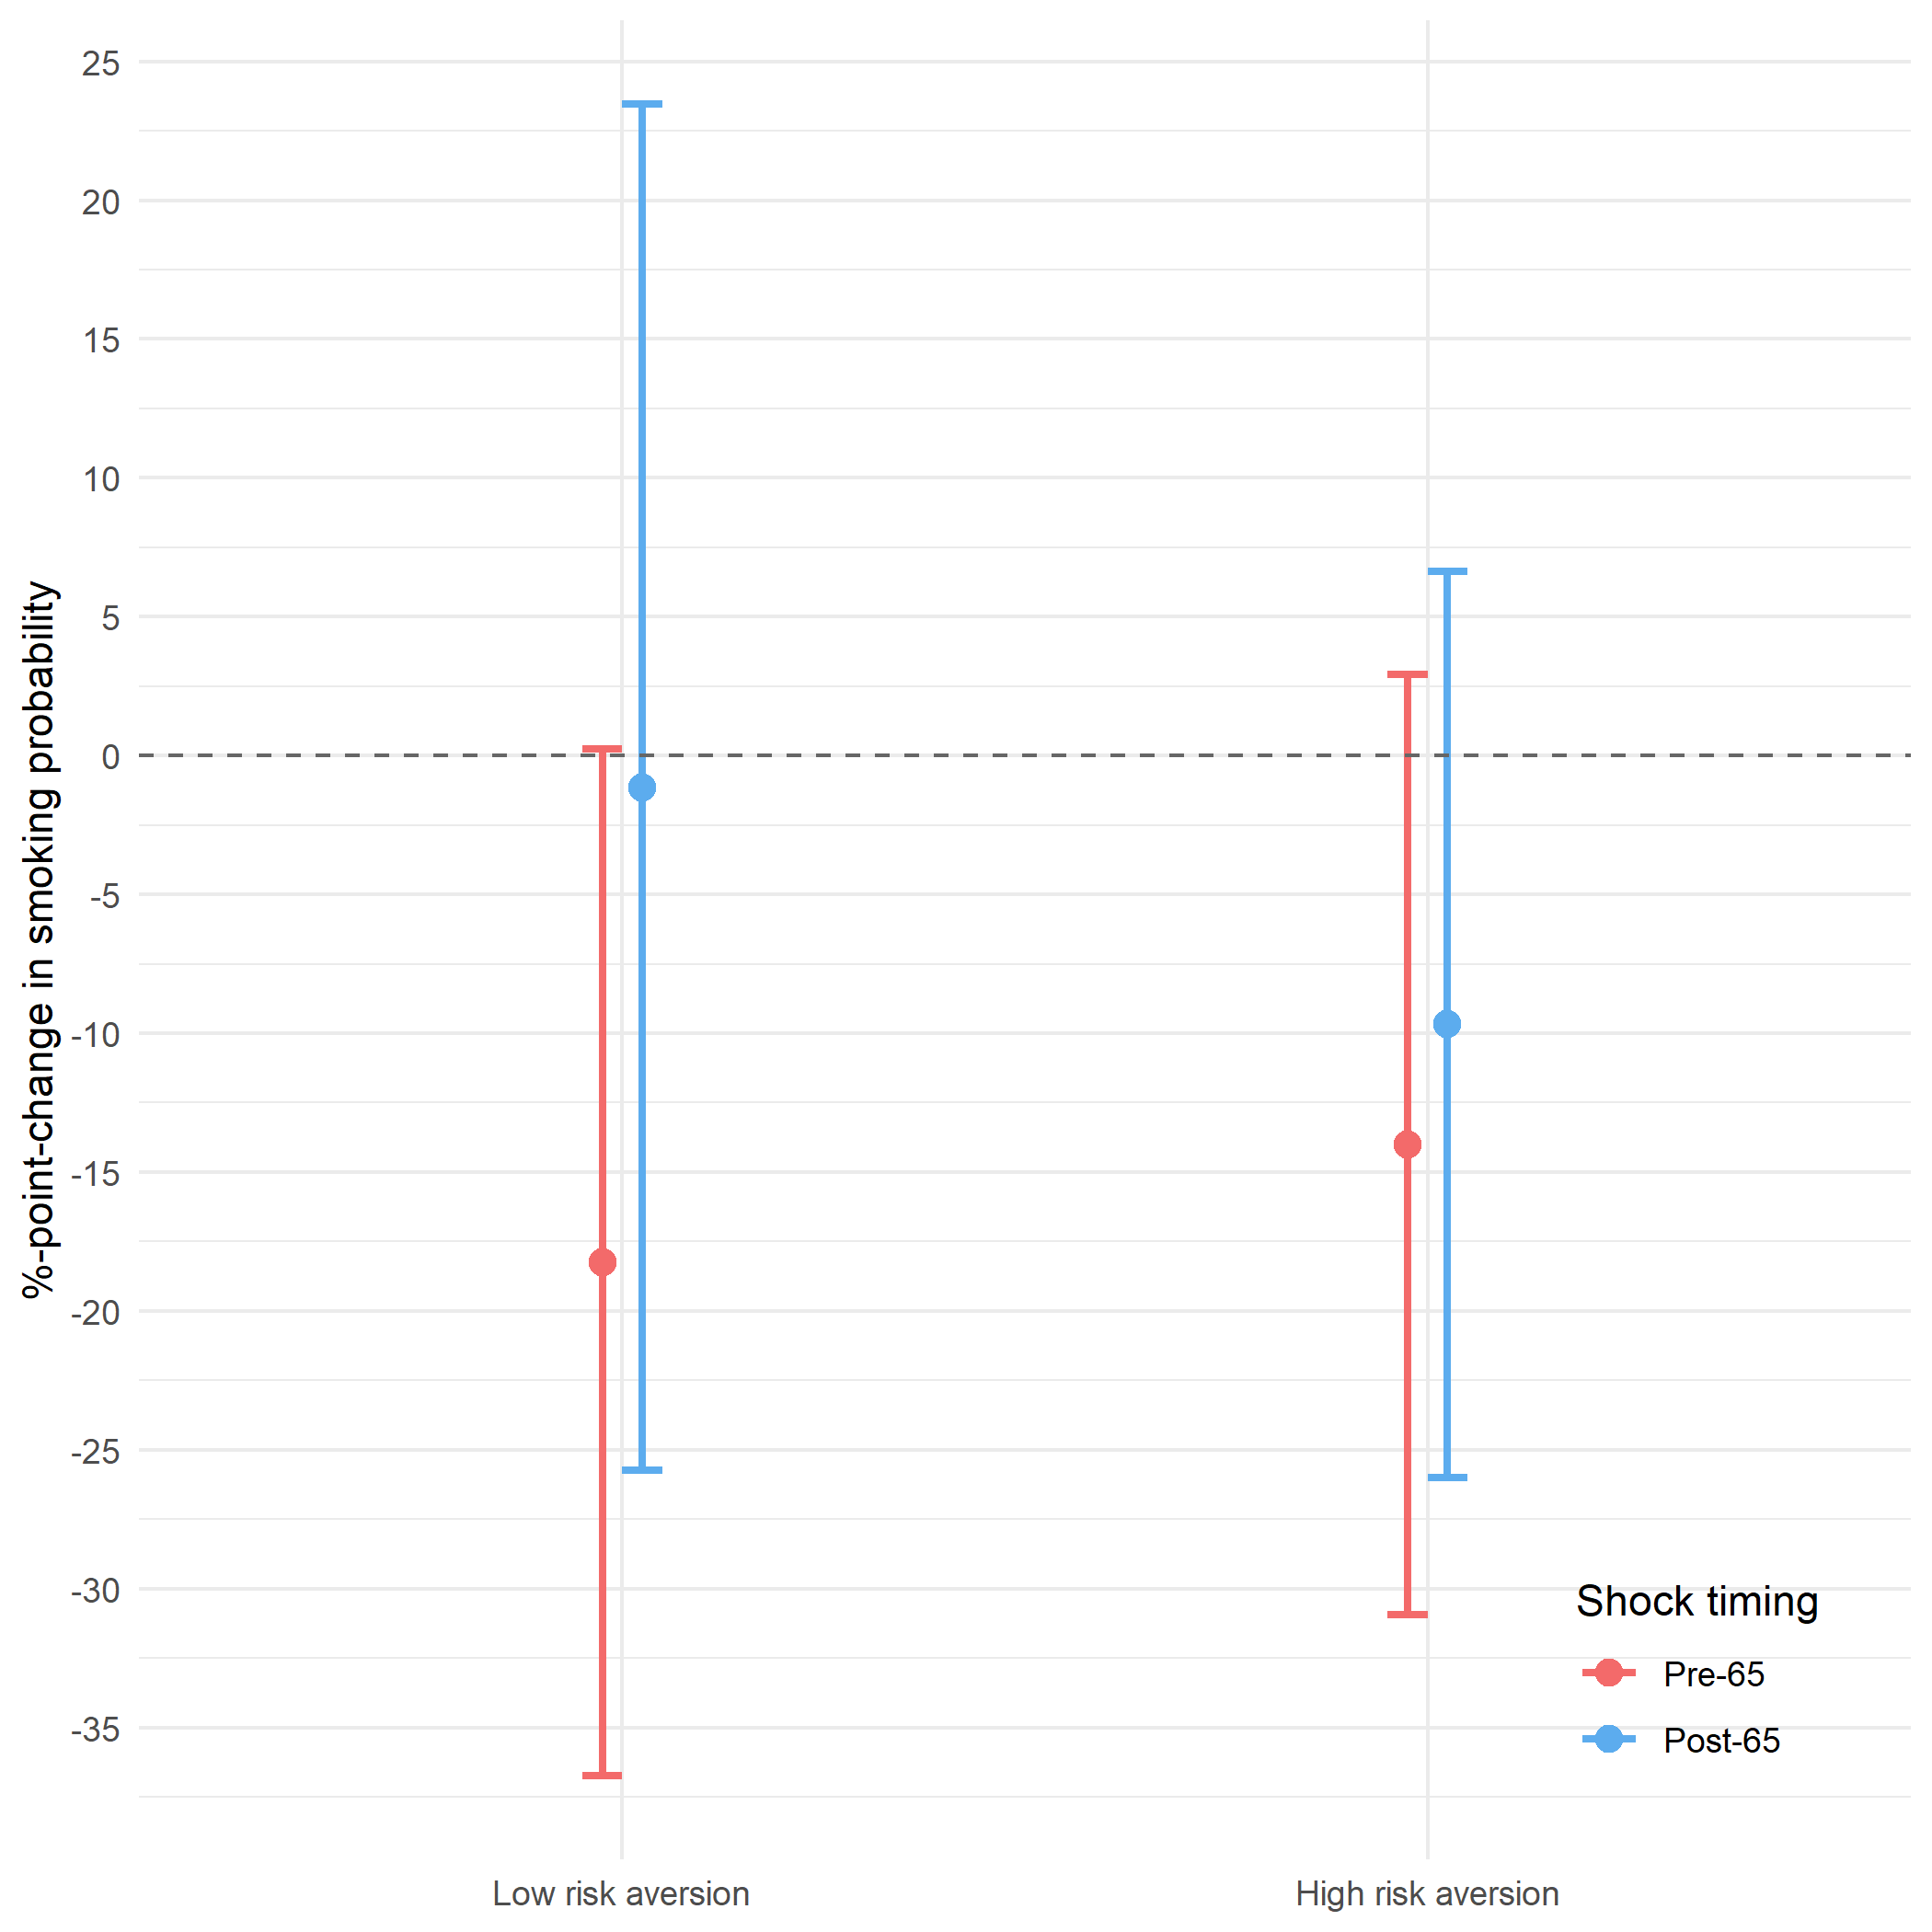
\includegraphics[height=0.8\textheight]{../../3_output/shock_effects/risk_6070_100_cv.png}
\label{fig:risk}
\end{figure}
\hyperlink{frame:otherX}{\beamergotobutton{back}}
\end{frame}
%--------------------------------------------------------------%
\begin{frame}
\frametitle{Split by gender}

\begin{figure}[hbtp]
\centering
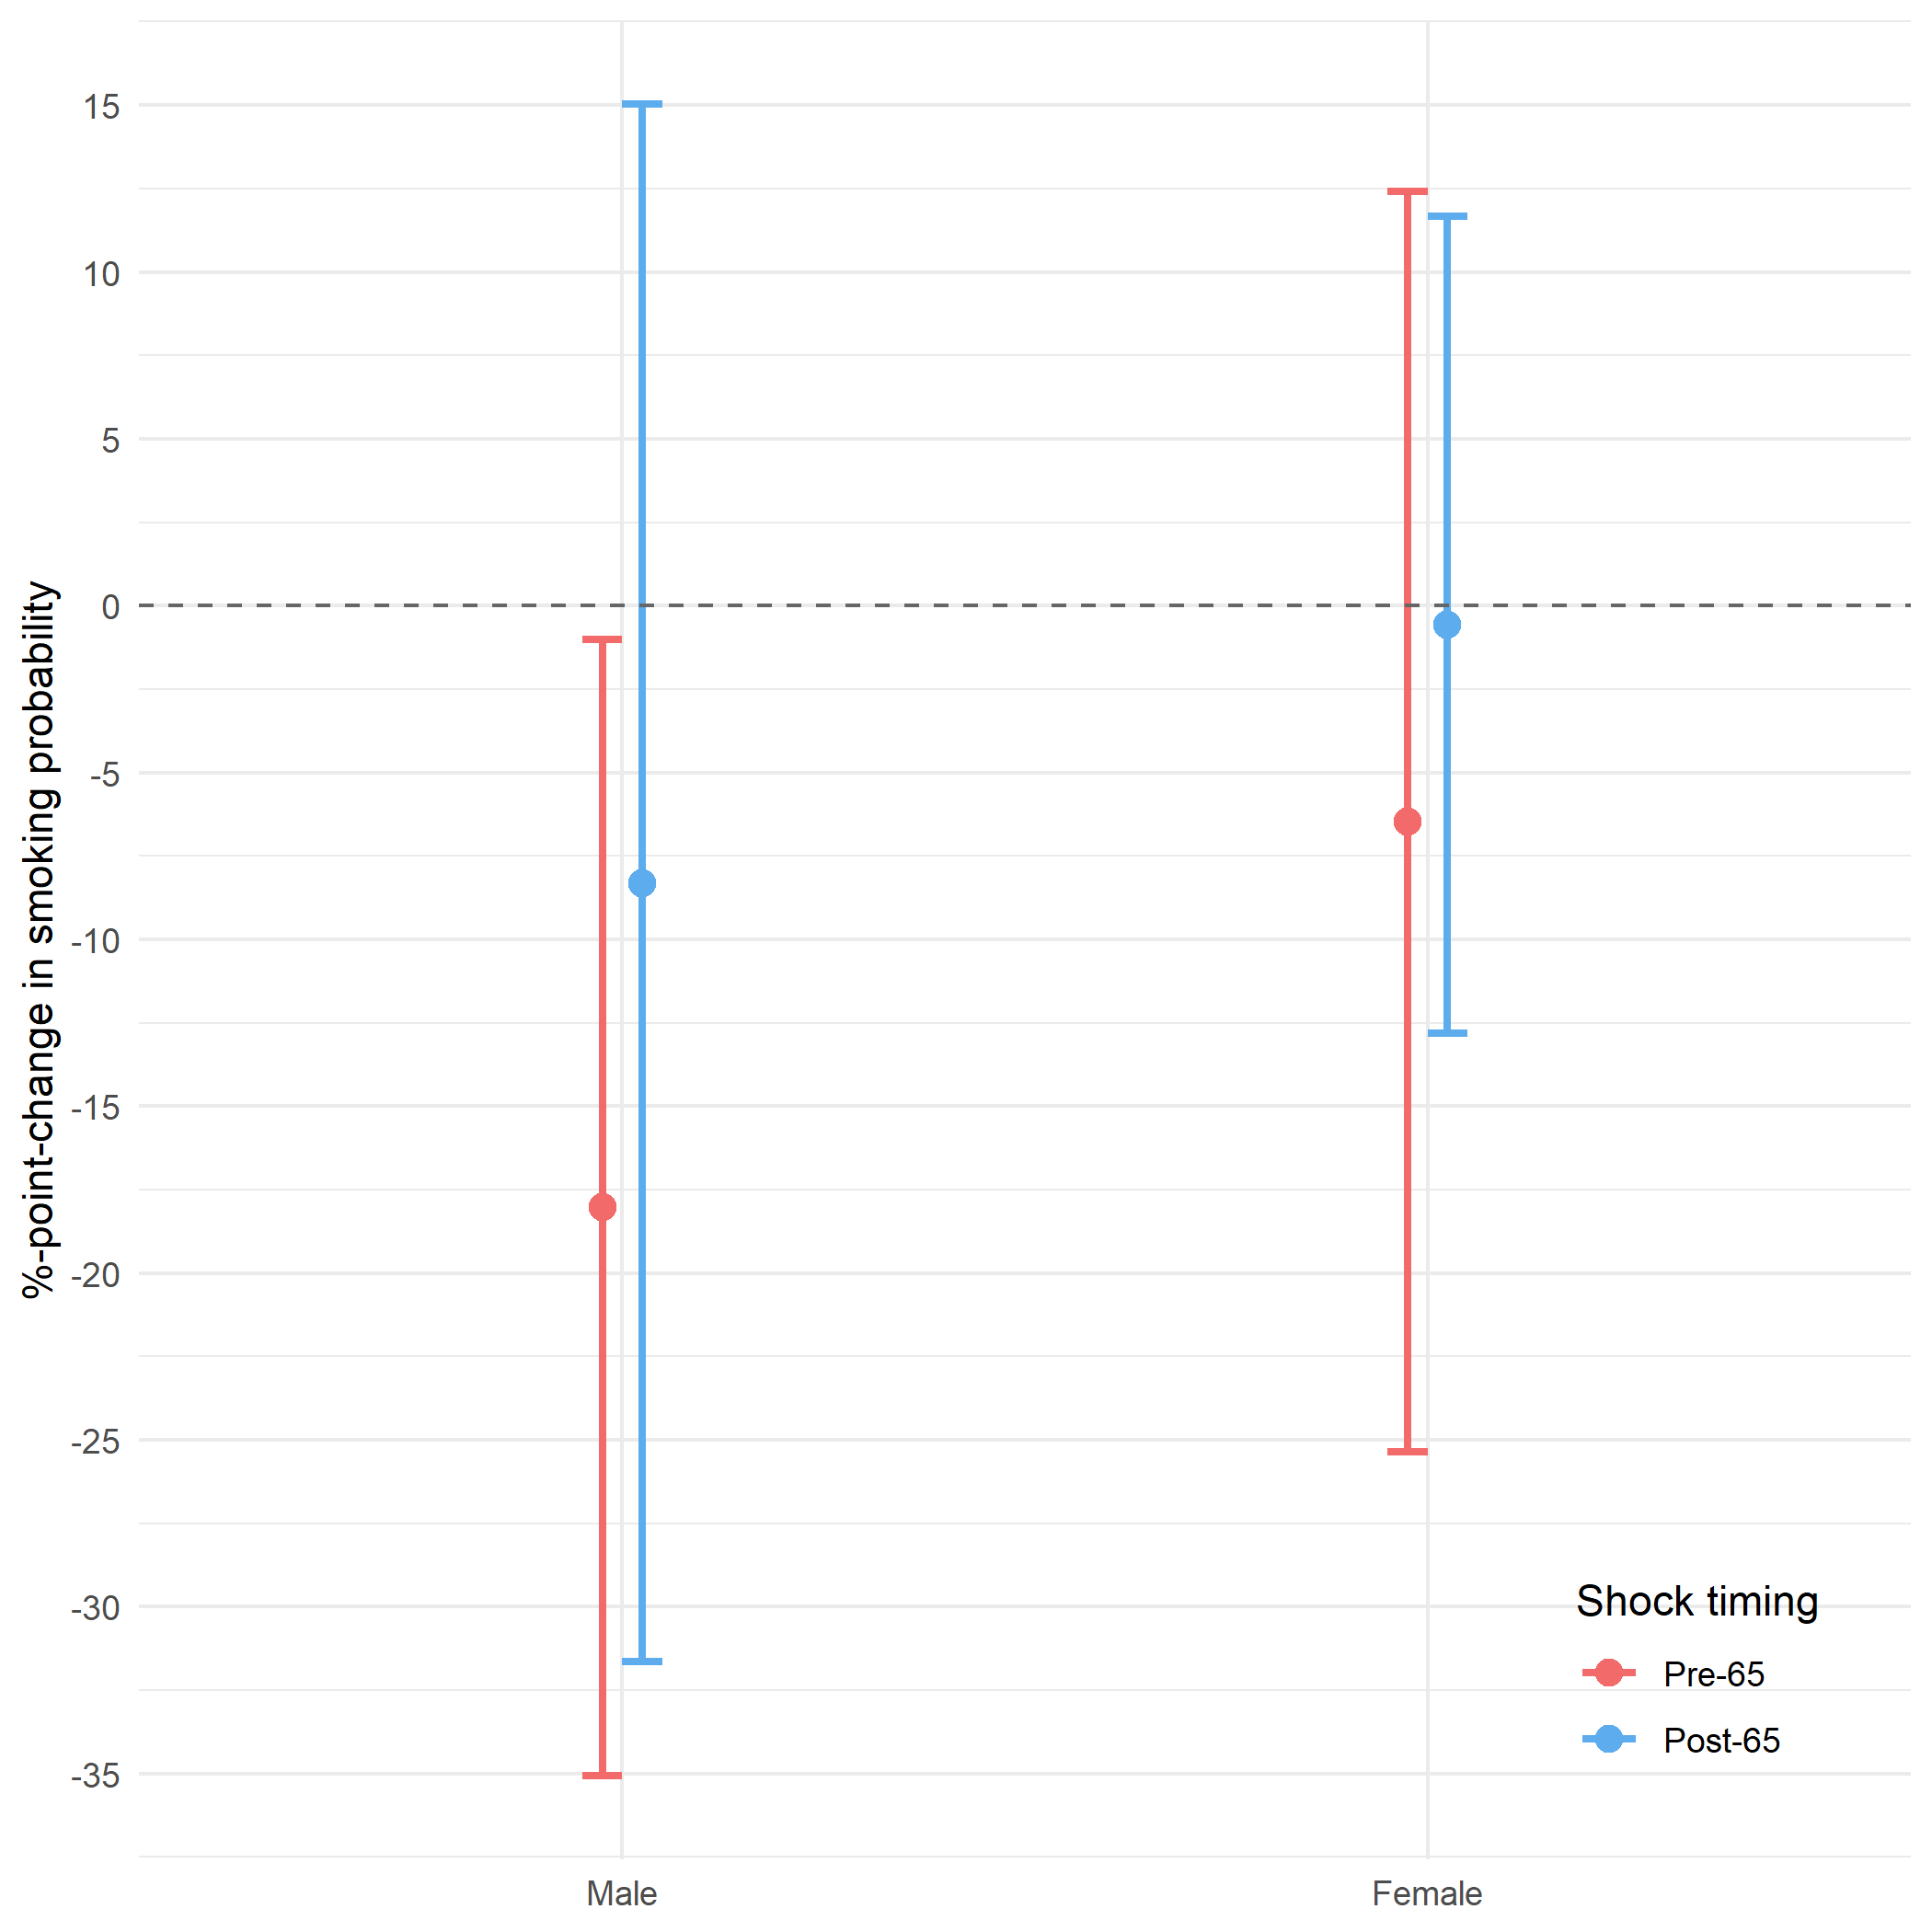
\includegraphics[height=0.8\textheight]{../../3_output/shock_effects/female_6070_100_cv.png}
\label{fig:female}
\end{figure}
\hyperlink{frame:otherX}{\beamergotobutton{back}}
\end{frame}
%--------------------------------------------------------------%
\begin{frame}
\frametitle{Split by education}

\begin{figure}[hbtp]
\centering
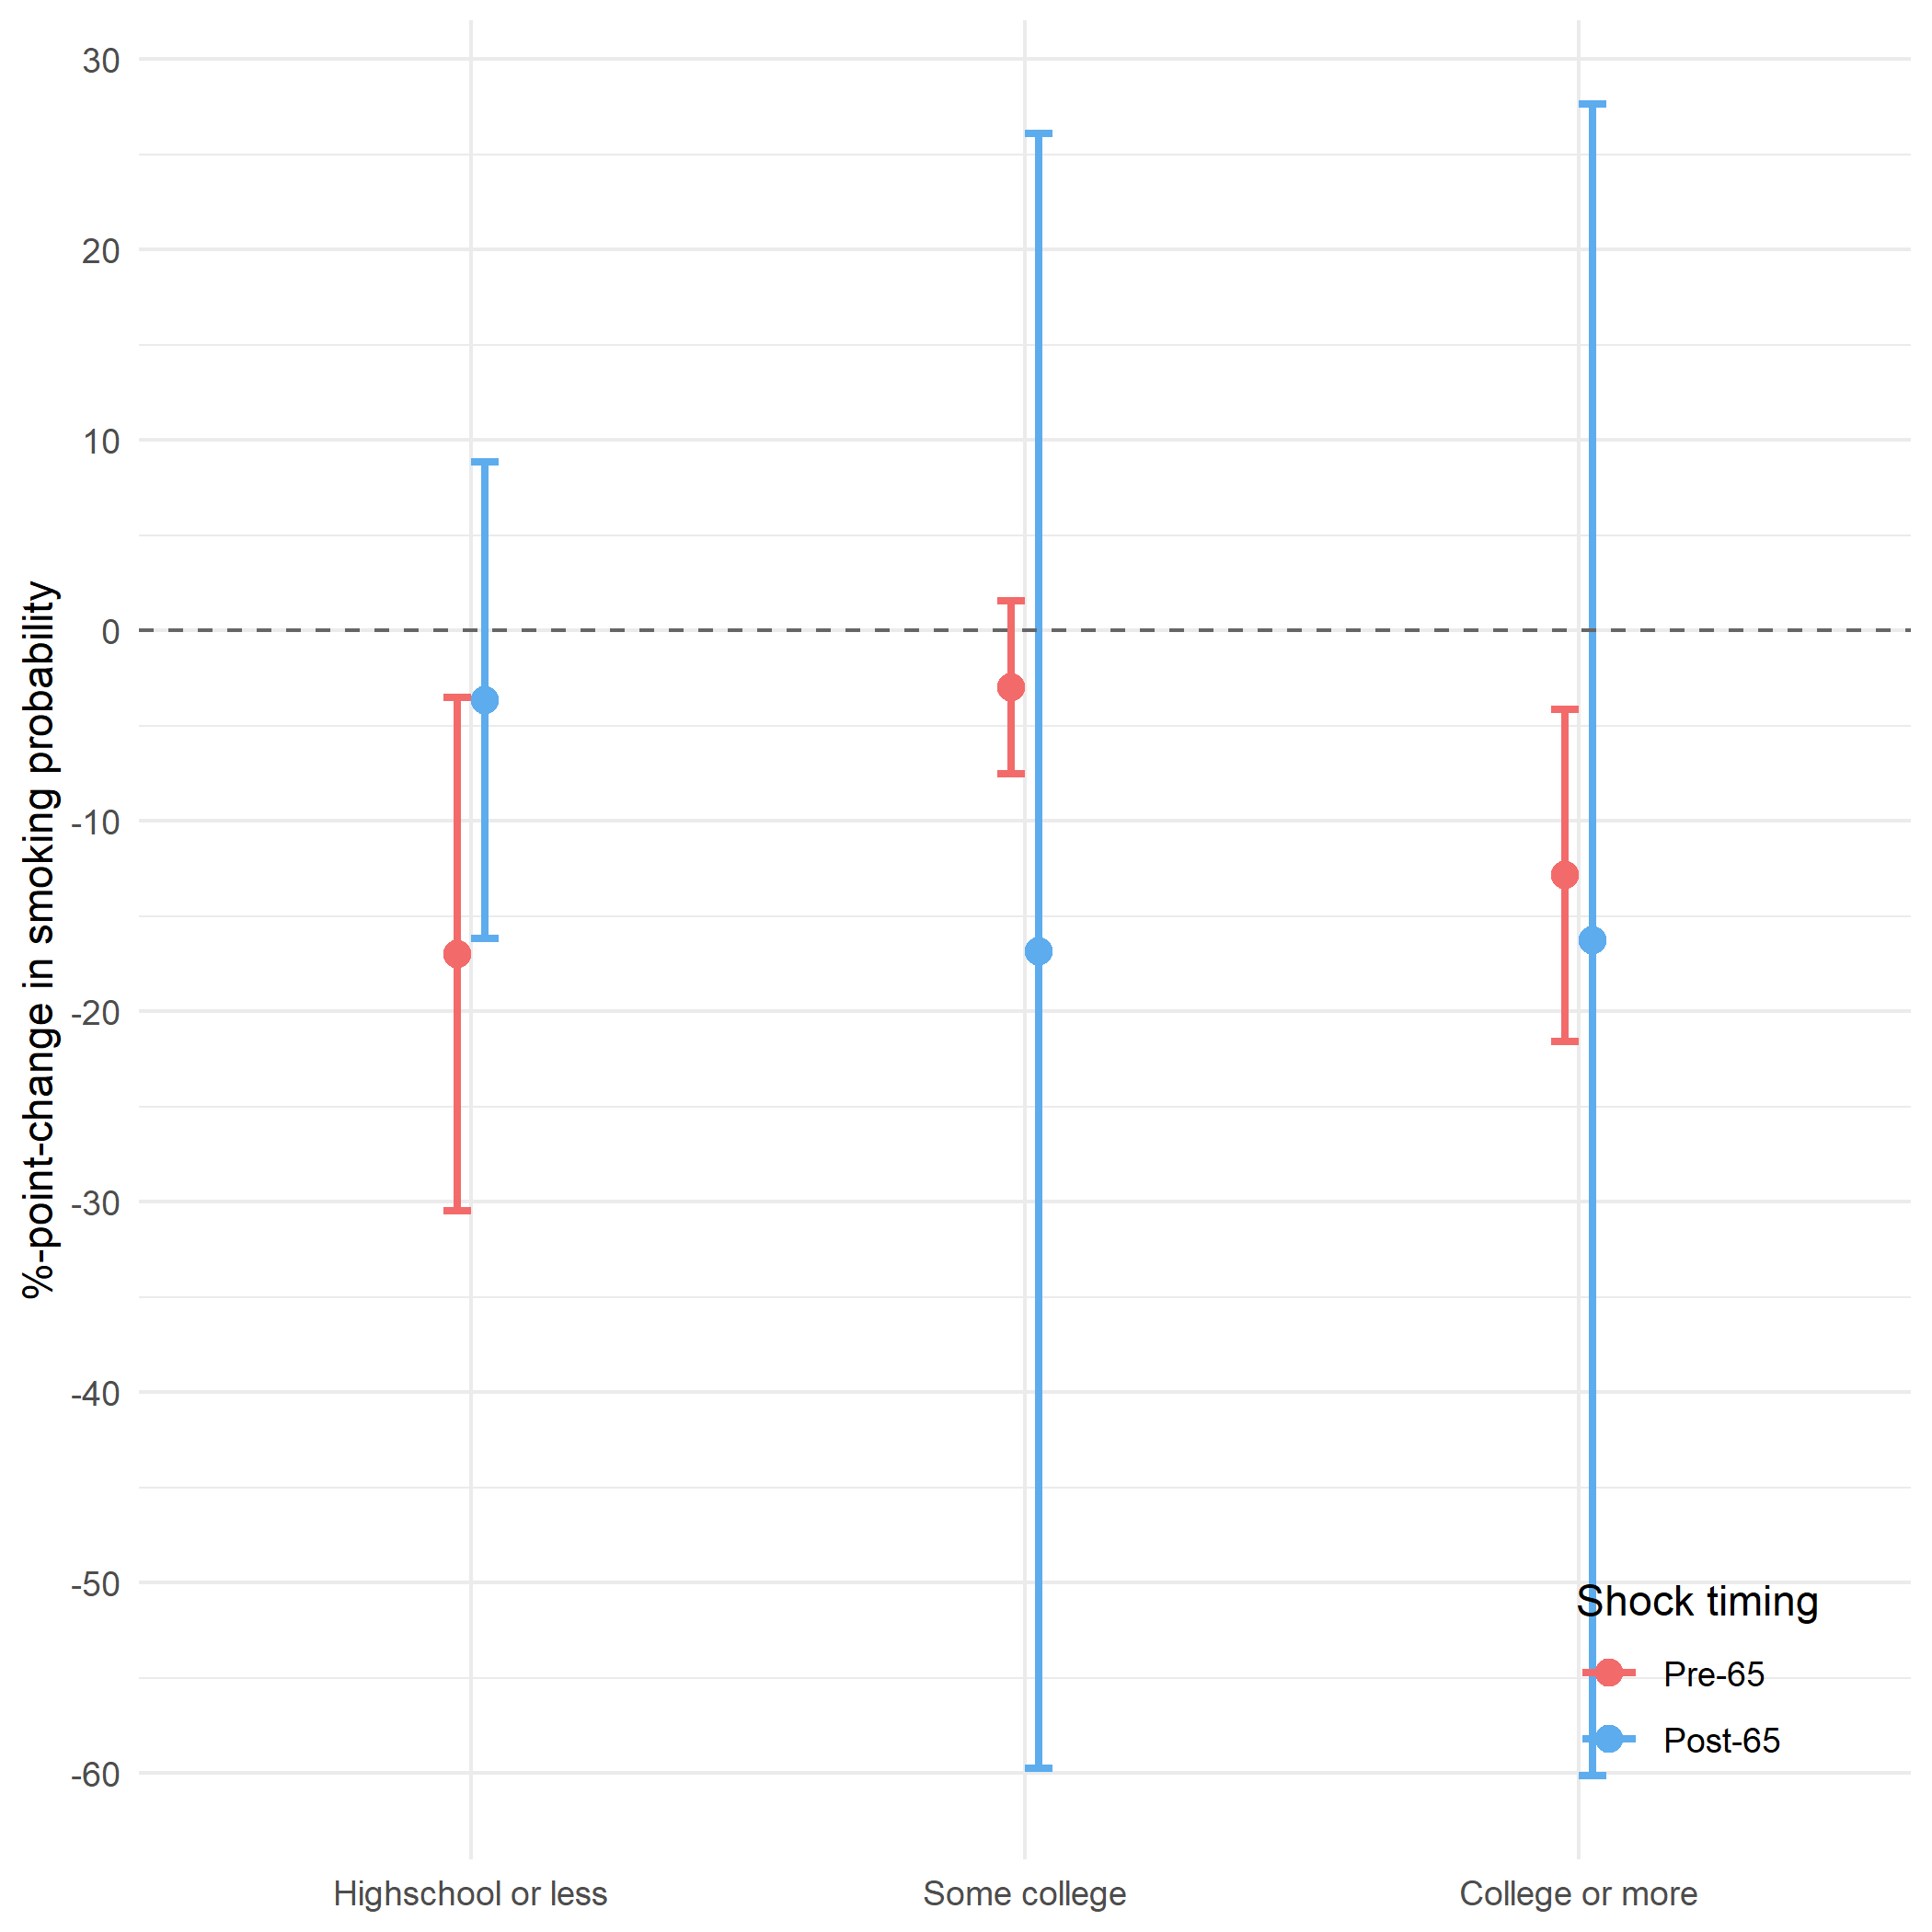
\includegraphics[height=0.8\textheight]{../../3_output/shock_effects/edu_6070_100_cv.png}
\label{fig:edu}
\end{figure}
\hyperlink{frame:otherX}{\beamergotobutton{back}}
\end{frame}
%--------------------------------------------------------------%
\begin{frame}
\frametitle{Split by former smoking behaviour}

\begin{figure}[hbtp]
	\centering
	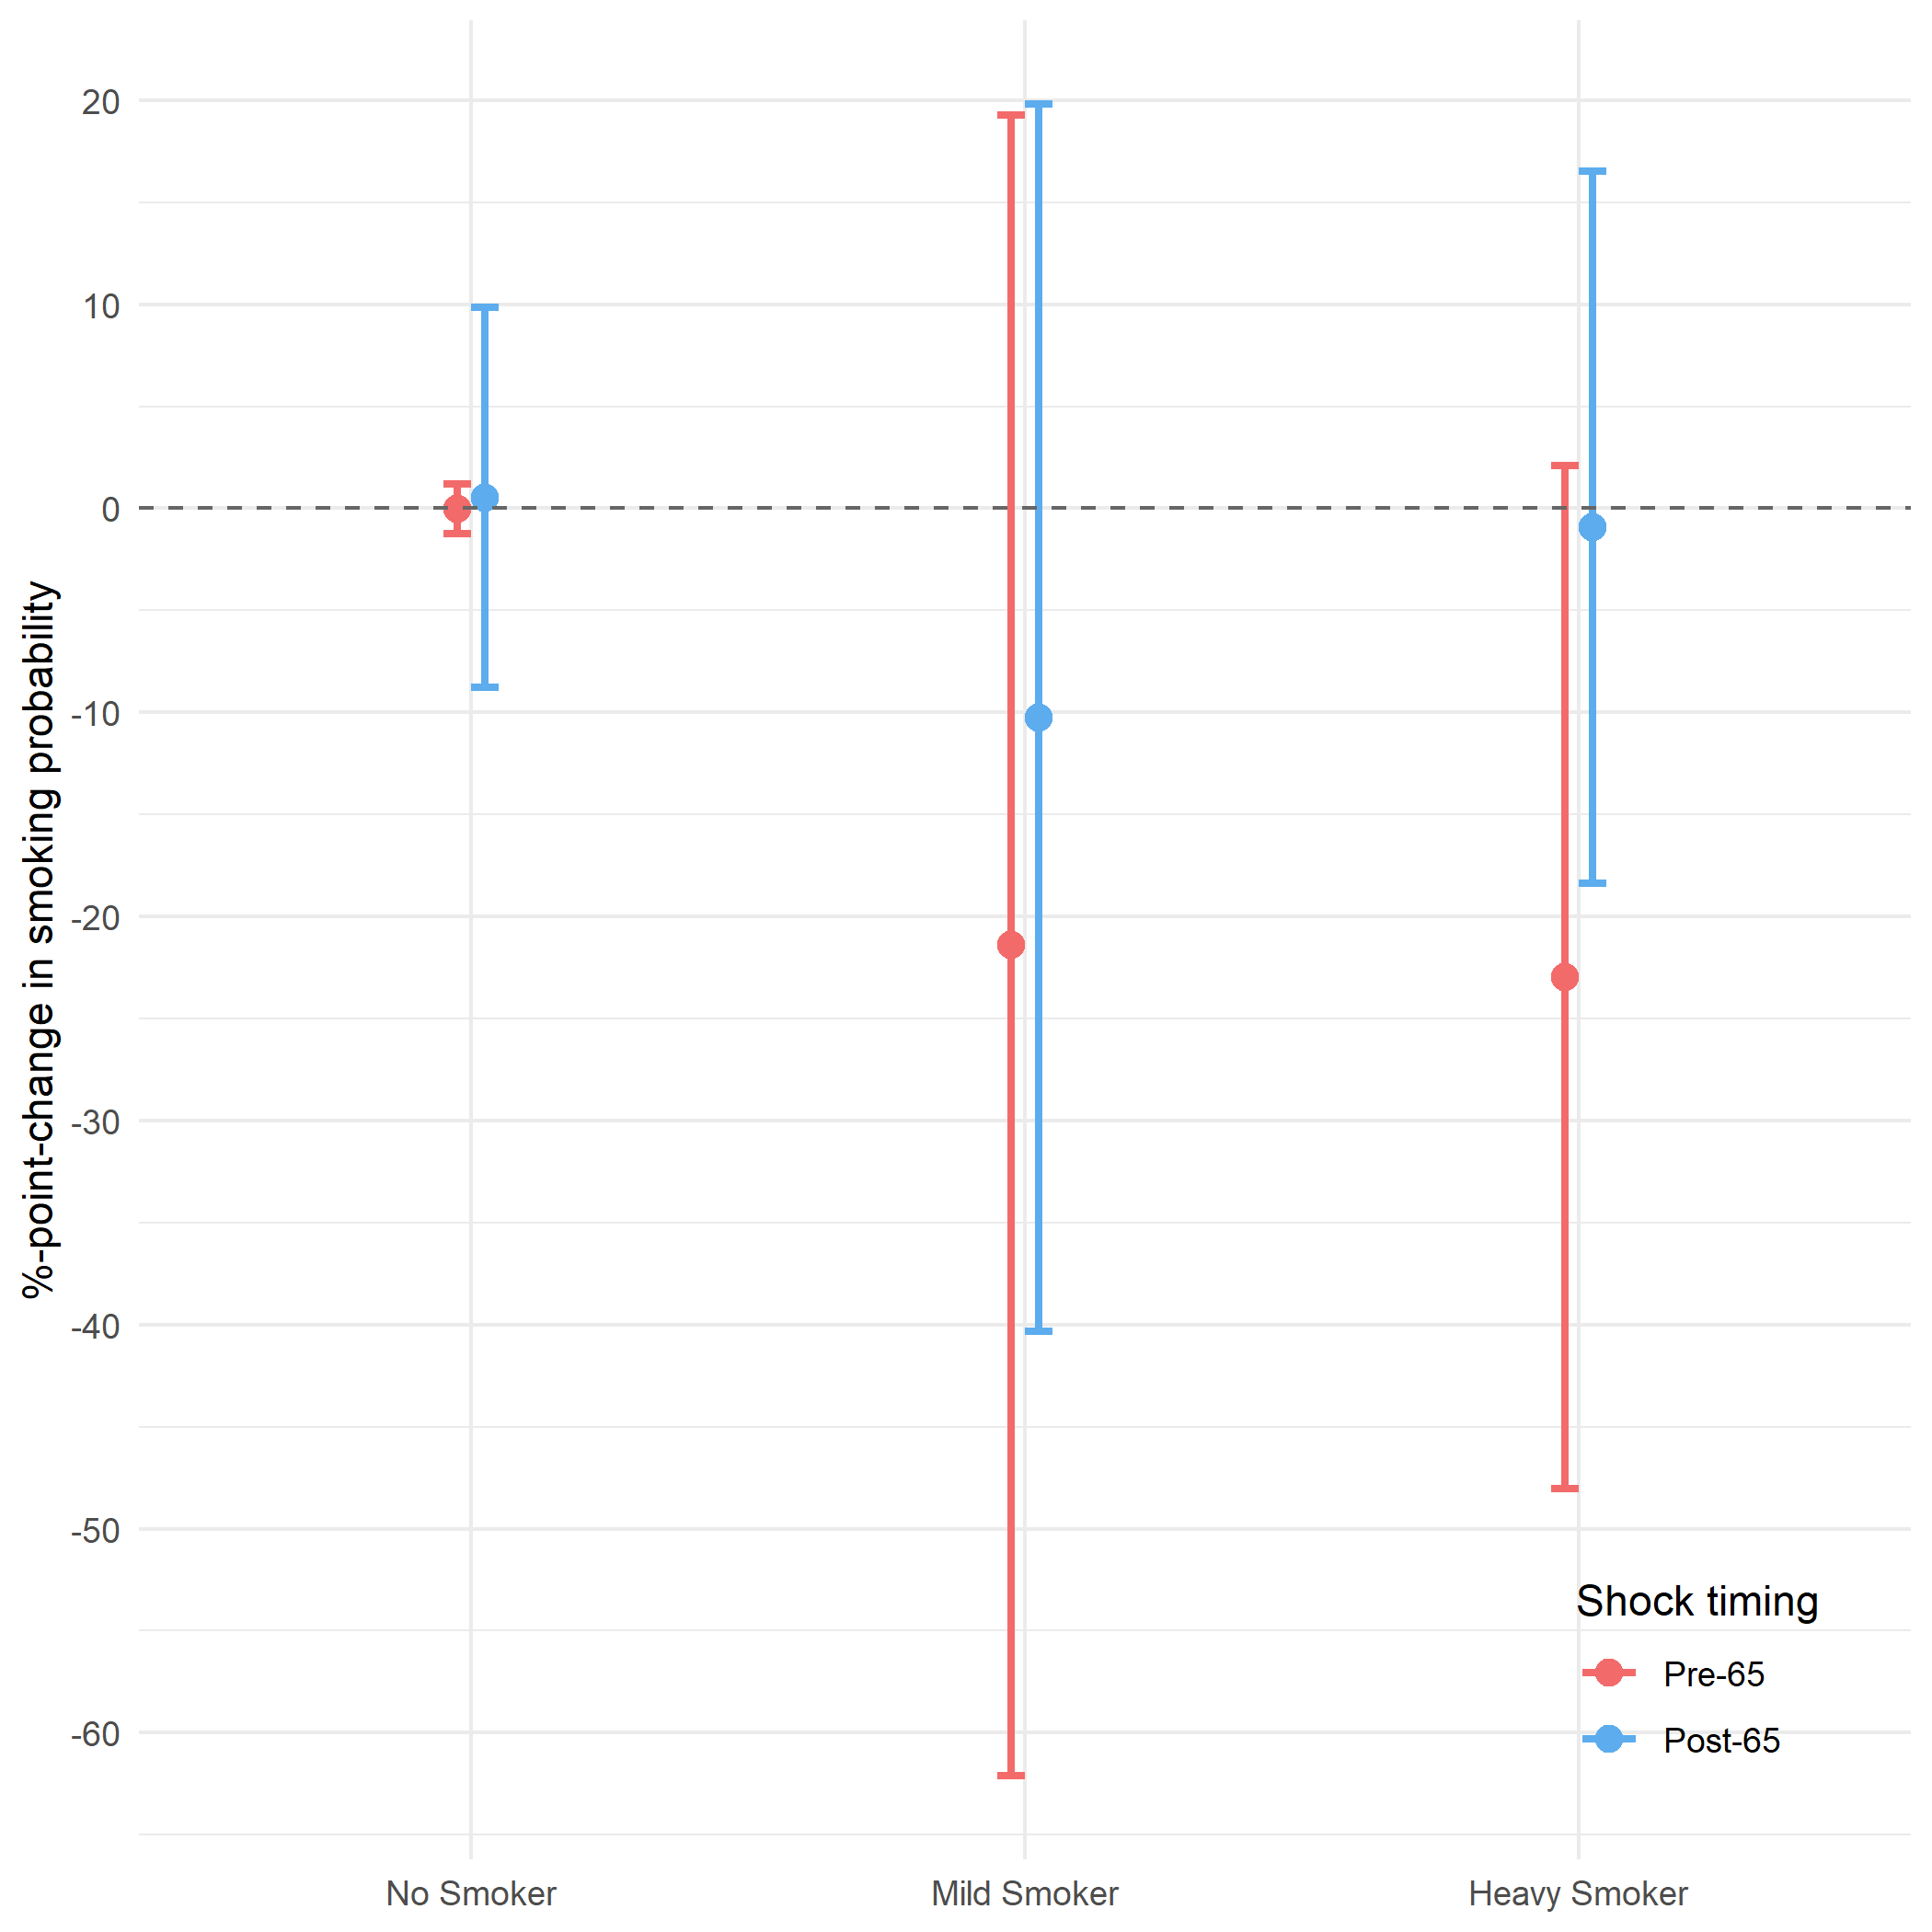
\includegraphics[height=0.8\textheight]{../../3_output/shock_effects/fSmokeB_6070_100_cv.png}
	\label{fig:edu}
\end{figure}
\hyperlink{frame:otherX}{\beamergotobutton{back}}
\end{frame}


%--------------------------------------------------------------%
\section{Conclusion}
%--------------------------------------------------------------%

\subsection{Limitations}
%--------------------------------------------------------------%
\begin{frame}{Limitations} \label{frame:limit}
Limitations:
\begin{itemize}
	\item Small sample size of those hit by a shock (replication needed) \hyperlink{frame:sumstats2}{\beamergotobutton{Sumstats2}}
	\item Short-run smoking response
	\item Self-reported information
	\item Unobserved selection into DNA-sample
%	\item Attrition and mortality not (yet) accounted for
%	\item Intensive margin (\# cig. smoked) not accounted for

	\vspace{3ex}
	\item External validity:
	\begin{itemize}
		\item U.S. insurance system
		\item Results only for old, uninsured people \hyperlink{frame:uninsured}{\beamergotobutton{sumstats}}
	\end{itemize}
\end{itemize}
\end{frame}

\subsection{Take home}
%--------------------------------------------------------------%
\begin{frame} \frametitle{Summary of Results}
\begin{itemize}
	\item Health shock when uninsured $\Rightarrow$ less smoking...
	\item ... but \textit{only} for low PGS.
	\item Effect size is quite sizable (27.9 pp)

	\vspace{3ex}

	\item Interaction between financial and ``biological'' constraints:
	\begin{itemize}
		\item Health insurance buffers financial consequences of health shocks
		\item Genetic predisposition to smoking mutes this effect (lower elasticity)
	\end{itemize}

	\vspace{3ex}

	\item Biological foundation of heterogeneity in \textbf{moral hazard} \cite{Einav2013}
\end{itemize}
\end{frame}


%=================================================================================

\begin{frame}{Conclusions}% and next steps}

What does this tell us?

\vspace{4ex}
\begin{itemize}
	\item Environment \emph{and} genes jointly influence healthy behaviors
	\vspace{2ex}
	\item Biological predispositions can tell a story about choices and economic fundamentals
	%\item $GxE$ can shed light on mechanisms at play
\end{itemize}

\end{frame}

%=================================================================================
\begin{frame}
\begin{center}
{\Huge \color{Verde}{Thank you}}
\end{center}
\end{frame}


%=================================================================================

%%--------------------------------------------------------------%
%\begin{frame}
%\frametitle{Questions}
%\begin{itemize}
%	\item Very small sample (hit by a shock): ex-post power calculations?
%	\item Attrition and mortality: how to best account for it?
%	\item Intensive margin (\# cig. smoked):
%	\begin{itemize}
%		\item Using different PGS
%		\item maybe tobit model?
%	\end{itemize}
%
%
%	\vspace{3ex}
%
%\begin{scriptsize}
%	\item Strange sumstats (see Table 1):
%	\begin{itemize}
%		\begin{scriptsize}
%		\item PGS higher for women \textit{only in analytic sample}
%		\item Age at baseline higher for those having a shock post-65
%		\item Number of waves present
%		\end{scriptsize}
%	\end{itemize}
%	\item Should control for more than age? income/wealth/family etc..
%	\item Not sure why s.e. is so small on Figure \ref{fig:maincoeffplot}
%\end{scriptsize}
%\end{itemize}
%
%\end{frame}

%--------------------------------------------------------------%
\appendix
\section{Appendix: Genetics of Smoking}
\subsection{App: Smoking and Mortality}
%%=================================================================================
%\begin{frame}{Causes of mortality}
%\begin{figure}
%  \centering
%    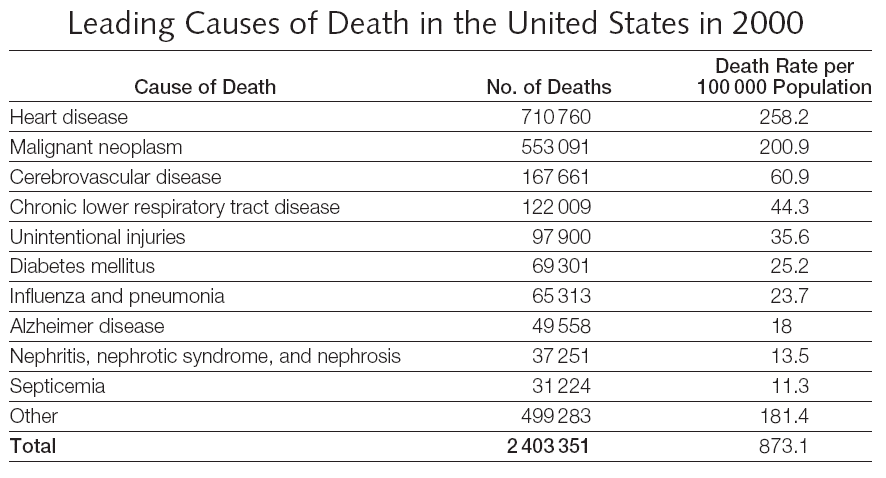
\includegraphics[width=1.0\textwidth]{Mokdad_leadingcauses.png}
%  \caption{\cite{Mokdad2004}}
%\end{figure}
%
%\end{frame}
%
%
%%=================================================================================
%
%\begin{frame}{Actual preventable causes of mortality}
%\begin{figure}
%  \centering
%    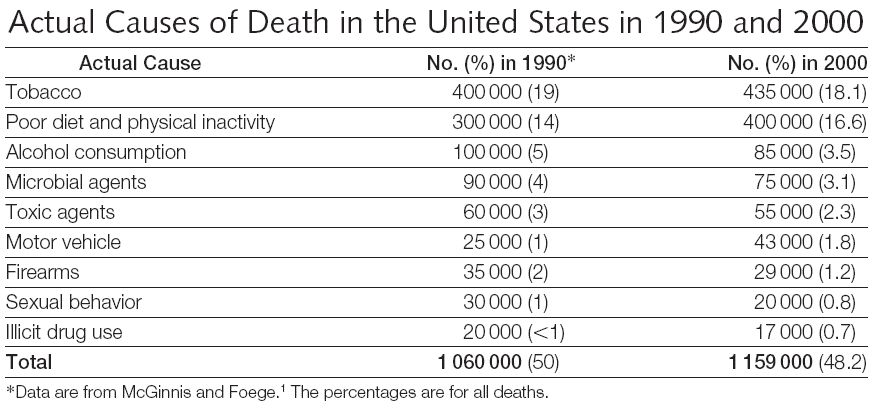
\includegraphics[width=1.0\textwidth]{Mokdad_actualcauses.png}
%  \caption{\cite{Mokdad2004}}
%\end{figure}
%
%\end{frame}
%
%%=================================================================================
%
%\begin{frame}%{The biological pathways of the nicotine receptor gene}
%\begin{figure}
%  \centering
%    \includegraphics[height=0.8\textheight]{arrows_smoking_addiction.pdf}
%\end{figure}
%
%\end{frame}
%
%=================================================================================

\begin{frame}{Smoking and lung cancer have same genetic hits}
\begin{figure}
  \centering
    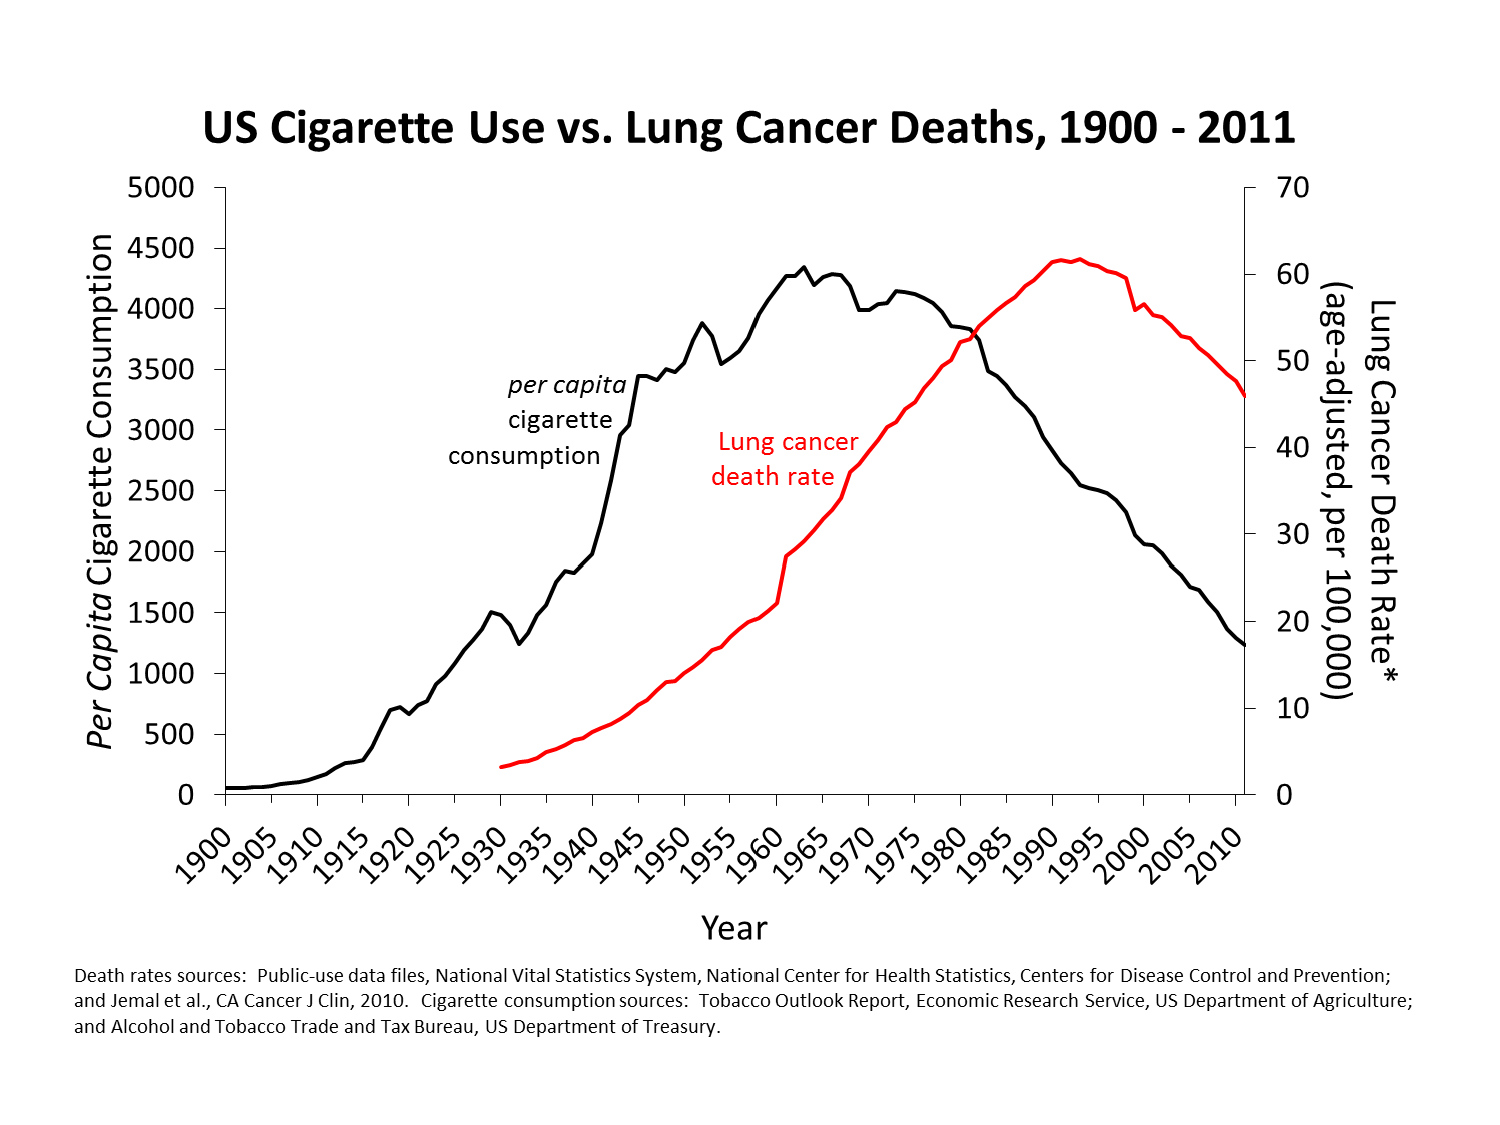
\includegraphics[height=0.8\textheight]{lung_cancer_rates.pdf}
\end{figure}

\end{frame}


%=================================================================================
\begin{frame}{Smoking and Obesity Manhattan Plots}
\begin{figure}
  \centering
    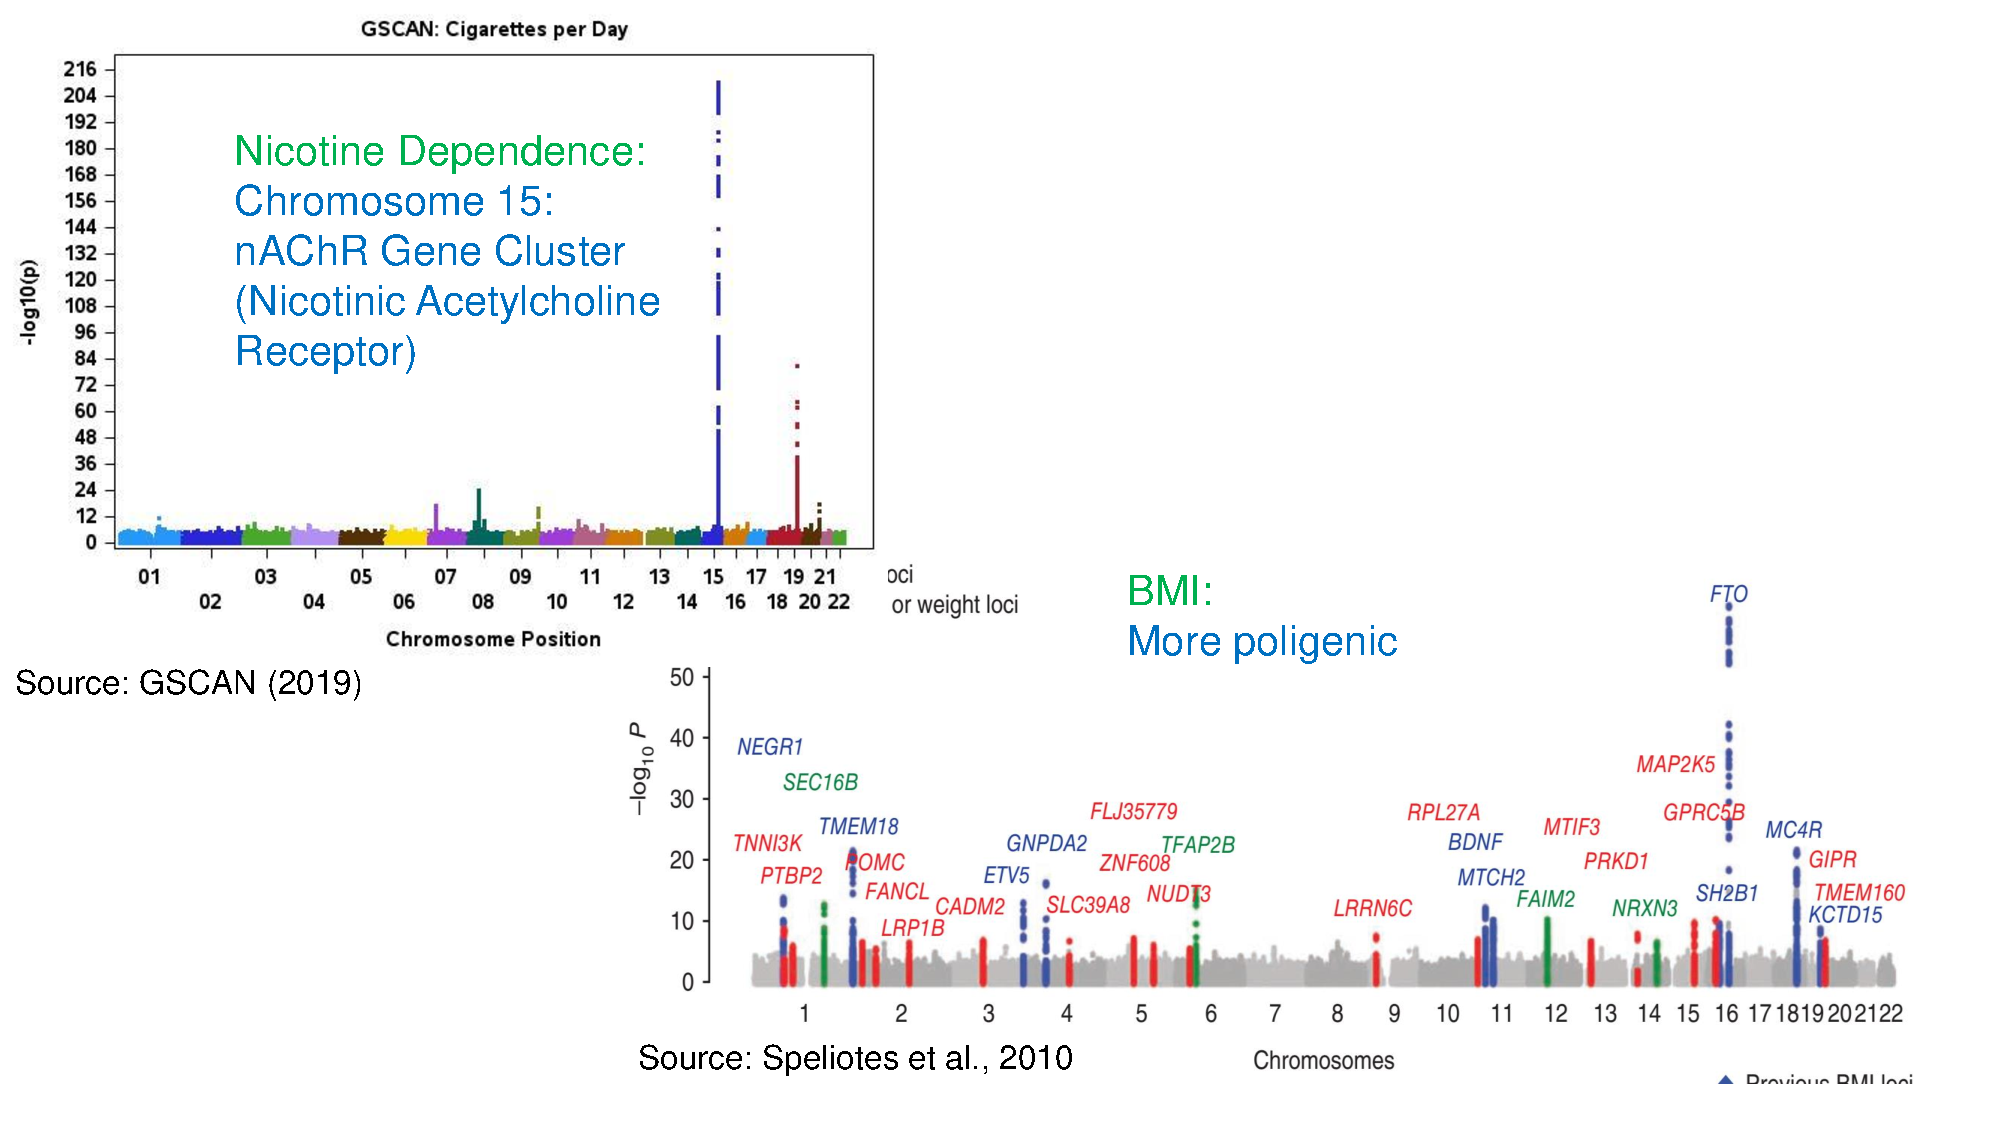
\includegraphics[height=0.8\textheight]{GWAS_manhattanplots.pdf}
  %\caption{Smoking and Obesity Manhattan Plots}
  \label{fig:manhattan2}
\end{figure}

\hyperlink{frame:genetics}{\beamergotobutton{back}}

\end{frame}

%=================================================================================

\begin{frame}{The biological pathways of the nicotine receptor gene}
\begin{figure}
  \centering
    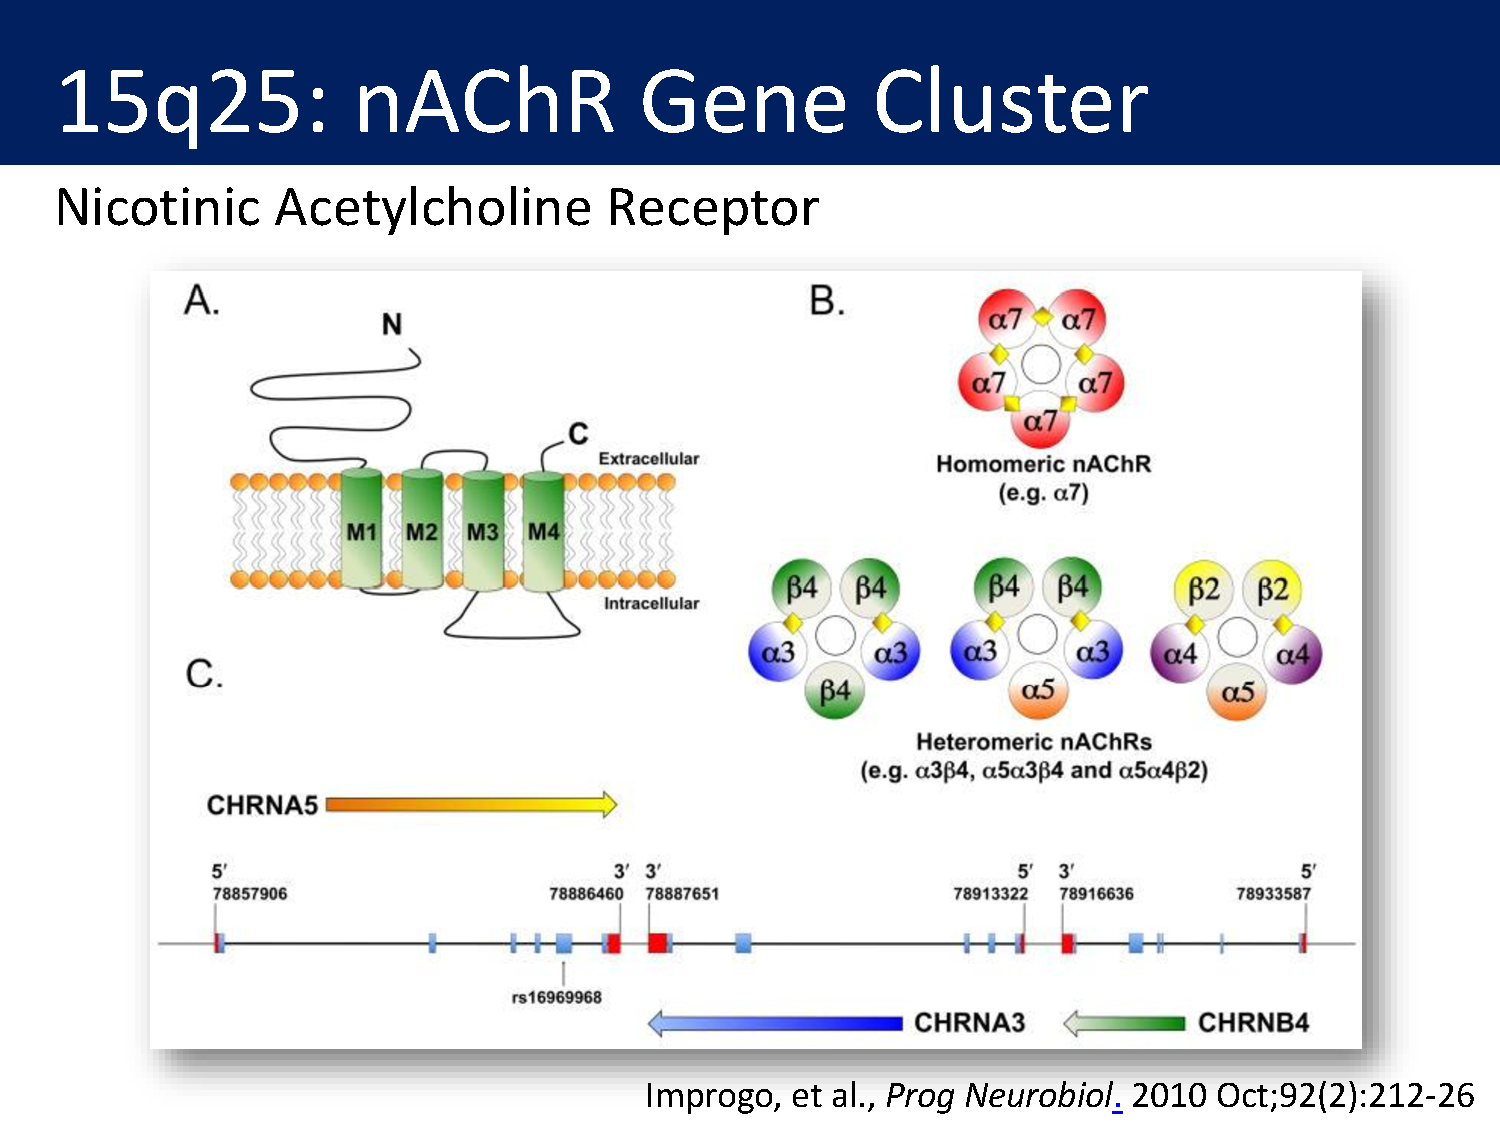
\includegraphics[height=0.8\textheight]{chr15q25_biology.pdf}
\end{figure}

\end{frame}


%--------------------------------------------------------------%
\subsection{App: Summary Statistics}
%--------------------------------------------------------------%
\begin{frame}
\frametitle{Summary statistics, by health shock timing}\label{frame:sumstats2}

\begin{table}[ht]
%	\caption{Descriptive Statistics for Subset of the Analytical Sample with a Health Shock, Stratified by Timing fo the Shock and Genetic Group}
	\small\resizebox{0.8\textheight}{!}{
		% latex table generated in R 4.0.2 by xtable 1.8-4 package
% 
\begin{tabular}{llll}
  \toprule
\textbf{  } & \textbf{ Low PGS } & \textbf{ High PGS } & \textbf{ P value } \\ 
  \midrule
Shock at ages 60-64 &  &  &  \\ 
   \midrule
 & Mean (SD) & Mean (SD) &  \\ 
  Age (baseline) & 60.49 (0.57) & 60.46 (0.62) & 0.67 \\ 
  Smoking PGS & -0.97 (0.54) & 0.63 (0.68) & 0.00 \\ 
  Years of education & 12.17 (3.44) & 12.15 (3.12) & 0.95 \\ 
  Income (nominal \$ 1000) & 19.61 (27.99) & 18.9 (30.1) & 0.83 \\ 
  No. waves present & 4.65 (1.31) & 4.59 (1.31) & 0.66 \\ 
   & \% & \% &  \\ 
  Female & 48.21 & 45.26 & 0.60 \\ 
  Smoking (baseline) & 30.36 & 37.23 & 0.19 \\ 
  Persistently uninsured & 4.46 & 6.57 & 0.39 \\ 
  Avg. cessation rate (baseline smokers) & 11.95 & 12.09 & 0.96 \\ 
  No. of individuals & 112 & 274 &  \\ 
   \midrule
No. of Person-year individuals & 521 & 1257 &  \\ 
   \midrule
Shock at ages 67-70 &  &  &  \\ 
   & Mean (SD) & Mean (SD) &  \\ 
  Age (baseline) & 61.16 (1.9) & 61.01 (1.22) & 0.44 \\ 
  Smoking PGS & -0.94 (0.48) & 0.76 (0.8) & 0.00 \\ 
  Years of education & 12.73 (3.15) & 12.42 (3.07) & 0.40 \\ 
  Income (nominal \$ 1000) & 17.75 (27.24) & 16.1 (20.41) & 0.58 \\ 
  No. waves present & 5.13 (1.05) & 5.13 (0.75) & 0.99 \\ 
   & \% & \% &  \\ 
  Female & 40.91 & 47.98 & 0.22 \\ 
  Smoking (baseline) & 28.18 & 34.98 & 0.21 \\ 
  Persistently uninsured & 8.18 & 6.28 & 0.54 \\ 
  Avg. cessation rate (baseline smokers) & 9.94 & 10.83 & 0.75 \\ 
   \midrule
No. of individuals & 110 & 223 &  \\ 
  No. of Person-year individuals & 564 & 1143 &  \\ 
  \end{tabular}

	}
\end{table}

%\begin{figure}[hbtp]

%\centering
%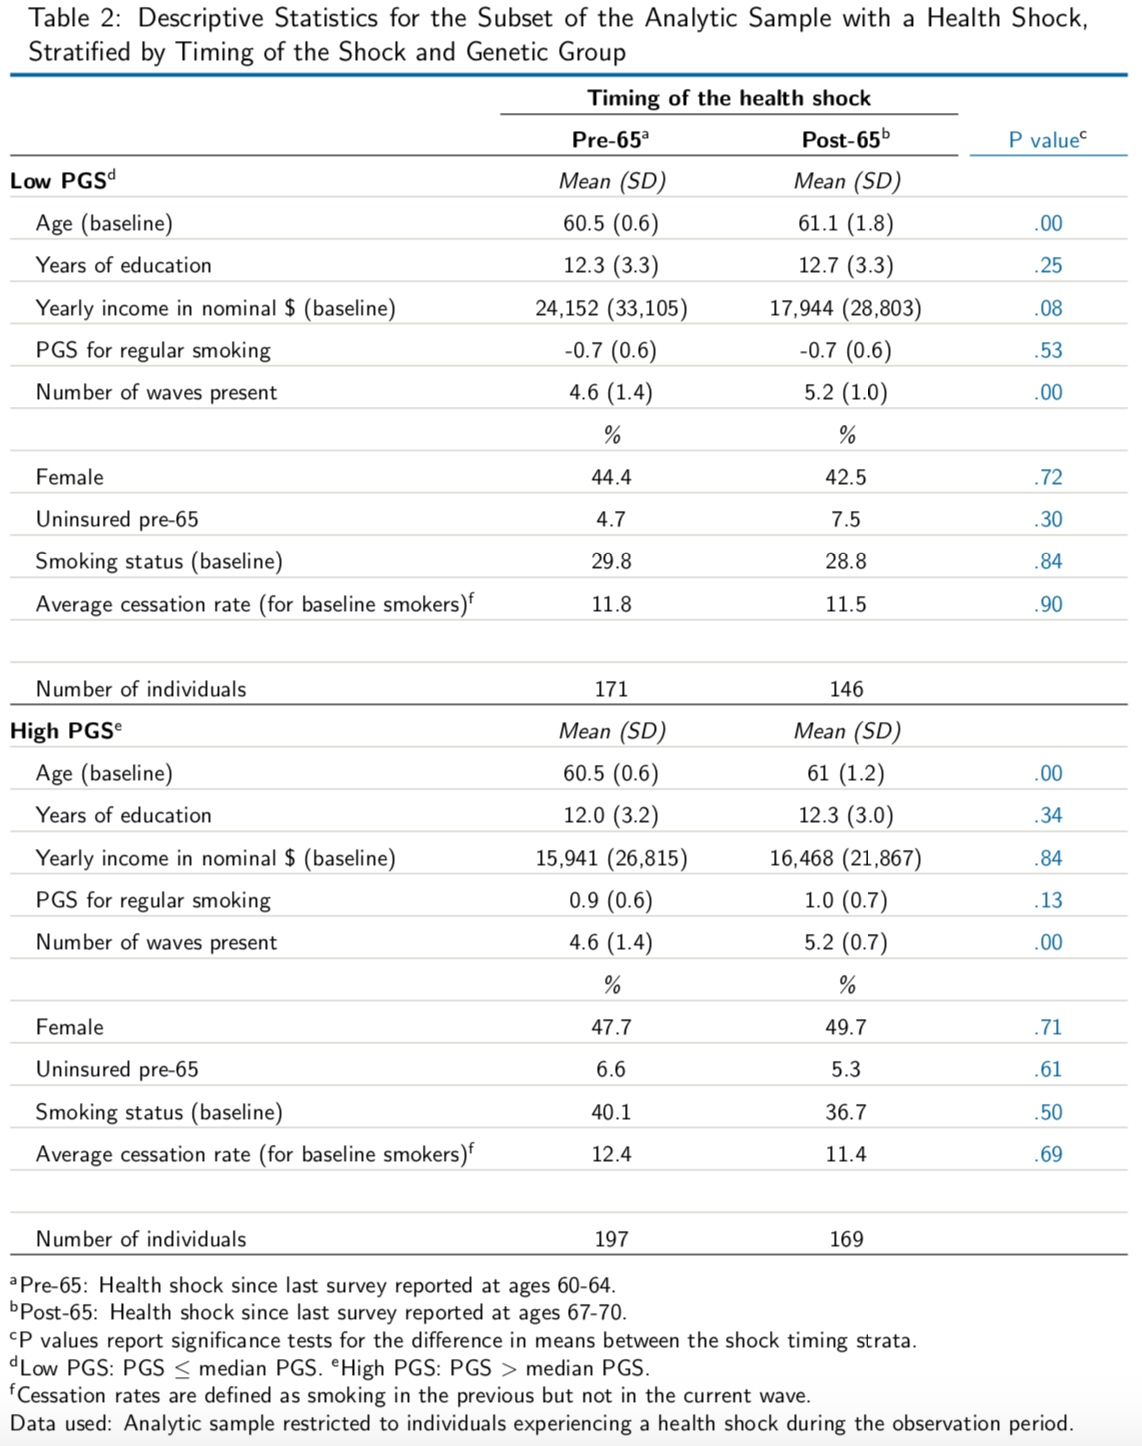
\includegraphics[height=0.8\textheight]{table2.png}
%\label{tab:sumstat2}
%\end{figure}

\hyperlink{frame:sumstats}{\beamergotobutton{back}}
\hyperlink{frame:limit}{\beamergotobutton{limitations}}
\end{frame}

%--------------------------------------------------------------%
\begin{frame}
\frametitle{Who are the uninsured?}\label{frame:uninsured}
\begin{table}[ht]
	\caption{Descriptive Statistics for Full Analytic Sample Stratified by Insurance Status}
	\small\resizebox{1.3\textheight}{!}{
		% latex table generated in R 4.0.2 by xtable 1.8-4 package
% 
\begin{tabular}{lllll}
  \toprule
\textbf{  } & \textbf{ All } & \textbf{ Uninsured } & \textbf{ Insured } & \textbf{ P value } \\ 
  \midrule
 & Mean (SD) & Mean (SD) & Mean (SD) &  \\ 
   \midrule
Age (baseline) & 61.15 (1.87) & 60.89 (0.99) & 61.17 (1.91) & 0.00 \\ 
  Smoking PGS & 0.1 (0.99) & 0.19 (0.93) & 0.1 (1) & 0.07 \\ 
  Years of education & 12.48 (3.09) & 10.36 (3.58) & 12.61 (3.01) & 0.00 \\ 
  Income (nominal \$ 1000) & 20.41 (34.97) & 8.72 (13.23) & 21.13 (35.77) & 0.00 \\ 
  No. waves present & 4.45 (1.36) & 4.35 (1.26) & 4.45 (1.37) & 0.14 \\ 
   & \% & \% & \% &  \\ 
  Female & 49.86 & 55.81 & 49.49 & 0.02 \\ 
  Smoking (baseline) & 29.5 & 46.51 & 28.44 & 0.00 \\ 
  Persistently uninsured & 5.88 & 100 & 0 & - \\ 
  CV health shock & 12.28 & 13.37 & 12.21 & 0.54 \\ 
  Avg. cessation rate (baseline smokers) & 10.3 & 8.48 & 10.48 & 0.07 \\ 
  No. of individuals & 5854 & 344 & 5510 &  \\ 
   \midrule
No. of person-year individuals & 26022 & 24527 & 1495 &  \\ 
  \end{tabular}

	}
\end{table}

\hyperlink{frame:sumstats}{\beamergotobutton{back}}
\hyperlink{frame:vars}{\beamergotobutton{back}}

\end{frame}



\subsection{App: Regression Results}
%--------------------------------------------------------------%
\begin{frame}
\frametitle{Regression results} \label{frame:fullreg}
{\scriptsize Coefficients from Estimating the Linear Probability Model in Equation (2) Using OLS} \hyperlink{fig:maincoeffplot}{\beamergotobutton{back}}

\begin{table}[ht]
	%\caption{Coefficients from Estimating the Linear Probability Model in Equation (2) Using OLS}
	\resizebox{0.8\textheight}{!}{
		
% Table created by stargazer v.5.2.2 by Marek Hlavac, Harvard University. E-mail: hlavac at fas.harvard.edu
% Date and time: Thu, Mar 11, 2021 - 5:34:49 PM
% Requires LaTeX packages: dcolumn 
\begin{tabular}{@{\extracolsep{0pt}}lD{.}{.}{-3} D{.}{.}{-3} D{.}{.}{-3} D{.}{.}{-3} D{.}{.}{-3} } 
\\[-1.8ex]\hline 
\hline \\[-1.8ex] 
 & \multicolumn{5}{c}{\textit{Dependent variable:}} \\ 
\cline{2-6} 
\\[-1.8ex] & \multicolumn{5}{c}{Smoking status} \\ 
\\[-1.8ex] & \multicolumn{1}{c}{(1)} & \multicolumn{1}{c}{(2)} & \multicolumn{1}{c}{(3)} & \multicolumn{1}{c}{(4)} & \multicolumn{1}{c}{(5)}\\ 
\hline \\[-1.8ex] 
 Health Shock & -0.026 & -0.026 & -0.026 & -0.050^{**} & -0.050^{**} \\ 
  & (0.040) & (0.040) & (0.040) & (0.023) & (0.023) \\ 
  & & & & & \\ 
 Post-65 & -0.066^{***} & -0.021^{*} & -0.021^{*} & -0.011 & -0.011 \\ 
  & (0.008) & (0.013) & (0.013) & (0.008) & (0.008) \\ 
  & & & & & \\ 
 Uninsured & 0.171^{***} & 0.171^{***} & 0.171^{***} &  &  \\ 
  & (0.027) & (0.027) & (0.027) &  &  \\ 
  & & & & & \\ 
 High PGS & 0.032^{**} & 0.032^{**} & 0.032^{**} &  &  \\ 
  & (0.012) & (0.013) & (0.013) &  &  \\ 
  & & & & & \\ 
 Shock $\times$ Post-65 & 0.014 & 0.023 & 0.022 & 0.022 & 0.022 \\ 
  & (0.055) & (0.056) & (0.056) & (0.032) & (0.032) \\ 
  & & & & & \\ 
 Shock $\times$ Uninsured & -0.198 & -0.192 & -0.193 & -0.115 & -0.117 \\ 
  & (0.184) & (0.184) & (0.184) & (0.073) & (0.073) \\ 
  & & & & & \\ 
 Post-65 $\times$ Uninsured & 0.067 & 0.065 & 0.065 & -0.052^{*} & -0.053^{*} \\ 
  & (0.048) & (0.048) & (0.048) & (0.032) & (0.032) \\ 
  & & & & & \\ 
 Shock $\times$ High PGS & 0.024 & 0.024 & 0.022 & 0.020 & 0.020 \\ 
  & (0.049) & (0.049) & (0.049) & (0.028) & (0.029) \\ 
  & & & & & \\ 
 Post-65 $\times$ High PGS & 0.001 & 0.001 & 0.001 & -0.003 & -0.003 \\ 
  & (0.010) & (0.010) & (0.010) & (0.008) & (0.008) \\ 
  & & & & & \\ 
 Shock $\times$ Post-65 x Uninsured & 0.286 & 0.280 & 0.280 & 0.233^{***} & 0.235^{***} \\ 
  & (0.250) & (0.251) & (0.250) & (0.086) & (0.085) \\ 
  & & & & & \\ 
 Shock $\times$ Uninsured $\times$ High PGS & 0.189 & 0.188 & 0.189 & 0.037 & 0.039 \\ 
  & (0.219) & (0.220) & (0.219) & (0.112) & (0.111) \\ 
  & & & & & \\ 
 Shock $\times$ Post-65 $\times$ High PGS & -0.048 & -0.048 & -0.046 & -0.077^{*} & -0.076^{*} \\ 
  & (0.068) & (0.068) & (0.068) & (0.042) & (0.042) \\ 
  & & & & & \\ 
 Post-65 $\times$ Uninsured $\times$ High PGS & -0.117^{*} & -0.117^{*} & -0.117^{*} & 0.043 & 0.043 \\ 
  & (0.062) & (0.062) & (0.062) & (0.037) & (0.037) \\ 
  & & & & & \\ 
 Shock $\times$ Post-65 $\times$ Uninsured $\times$ High PGS & -0.151 & -0.153 & -0.154 & -0.185 & -0.188 \\ 
  & (0.309) & (0.310) & (0.309) & (0.153) & (0.152) \\ 
  & & & & & \\ 
\hline \\[-1.8ex] 
Age & & Yes & Yes & Yes & Yes  \\
Year FE & &              & Yes &              & Yes  \\
Individual FE   & &              &              & Yes & Yes  \\
 \hline \\[-1.8ex]
Observations & \multicolumn{1}{c}{25,800} & \multicolumn{1}{c}{25,800} & \multicolumn{1}{c}{25,800} & \multicolumn{1}{c}{25,800} & \multicolumn{1}{c}{25,800} \\ 
R$^{2}$ & \multicolumn{1}{c}{0.016} & \multicolumn{1}{c}{0.017} & \multicolumn{1}{c}{0.017} & \multicolumn{1}{c}{0.822} & \multicolumn{1}{c}{0.822} \\ 
\hline 
\hline \\[-1.8ex] 
\end{tabular} 

	}
\end{table}

%\hyperlink{fig:maincoeffplot}{\beamergotobutton{back}}

\end{frame}

%--------------------------------------------------------------%
\begin{frame}
\frametitle{Meaning of OLS coefficients} \label{frame:OLSmath}
From estimating equation \ref{eq:OLS} we get the following:
\hyperlink{fig:maincoeffplot}{\beamergotobutton{back}}

\begin{footnotesize}
\begin{align}
\phantom{E\left[ Y_{it}| post65_{it}=1, g_i=1, shock_{it}=1,uninsured_i=1\right]}
&\begin{aligned}
	\mathllap{E\left[ Y_{it}| post65_{it}=0, g_i=0, shock_{it}=1,uninsured_i=1\right]} &=\beta+\lambda_2
\end{aligned}\\
&\begin{aligned}
	\mathllap{E\left[ Y_{it}| post65_{it}=1, g_i=0, shock_{it}=1,uninsured_i=1\right]} &=\beta+\gamma+\lambda_1+\lambda_2\\ &+\lambda_3+\delta_1
\end{aligned}\\
&\begin{aligned}
	\mathllap{E\left[ Y_{it}| post65_{it}=0, g_i=1, shock_{it}=1,uninsured_i=1\right]} &=\beta+\lambda_2+\lambda_4+\delta_2
\end{aligned}\\
&\begin{aligned}
	\mathllap{E\left[ Y_{it}| post65_{it}=1, g_i=1, shock_{it}=1,uninsured_i=1\right]} &=\beta+\gamma+\lambda_1+\lambda_2\\
	&+\lambda_3+\lambda_4+\lambda_5+\delta_1+\delta_2\\
	&+\delta_3+\delta_4+\xi
\end{aligned}
\end{align}

Then the first two differences yield:

\begin{align}
(2)-(1)&=\gamma+\lambda_1+\lambda_3+\delta_1\\
(4)-(3)&=\gamma+\lambda_1+\lambda_3+\lambda_5+\delta_1+\delta_3+\delta_4+\xi
\end{align}

And finally the diff-in-diff (G$\times$E) is identified by:
\begin{align}
	(6)-(5)&=\lambda_5+\delta_3+\delta_4+\xi
\end{align}
\end{footnotesize}

\end{frame}

%--------------------------------------------------------------%
\begin{frame}
\frametitle{Effect of the shock on the outcomes} \label{frame:shockmath2}
The derivative of the outcome with respect to shock is:
\hyperlink{fig:maincoeffplot}{\beamergotobutton{back}}

\begin{footnotesize}
\begin{align}
\begin{aligned}
	\frac{\partial Y_{it}}{\partial shock_{it}}&=\beta+\lambda_1post65_{it}+\lambda_2uninsured_{i}+\lambda_4g_i\\
	&+\delta_1(post65 \times uninsured_i)+\delta_2(uninsured_i \times g_i)+\delta_3(post65_{it} \times g_i)\\
	&+\xi(post65_{it} \times uninsured_i \times g_i)
\end{aligned}
\end{align}

Again, we can look at the decomposition:
\begin{align}
\phantom{E\left[ \frac{\partial Y_{it}}{\partial shock_{it}}| post65_{it}=1, g_i=1,uninsured_i=1\right]}
&\begin{aligned}
\mathllap{E\left[ \frac{\partial Y_{it}}{\partial shock_{it}}| post65_{it}=0, g_i=0,uninsured_i=1\right]} &=\beta+\lambda_2
\end{aligned}\\
&\begin{aligned}
\mathllap{E\left[ \frac{\partial Y_{it}}{\partial shock_{it}}| post65_{it}=1, g_i=0,uninsured_i=1\right]} &=\beta+\lambda_1+\lambda_2+\delta_1
\end{aligned}\\
&\begin{aligned}
\mathllap{E\left[ \frac{\partial Y_{it}}{\partial shock_{it}}| post65_{it}=0, g_i=1,uninsured_i=1\right]} &=\beta+\lambda_2+\lambda_4+\delta_2
\end{aligned}\\
&\begin{aligned}
\mathllap{E\left[ \frac{\partial Y_{it}}{\partial shock_{it}}| post65_{it}=1, g_i=1,,uninsured_i=1\right]} &=\beta+\lambda_1+\lambda_2+\lambda_4\\
&+\delta_1+\delta_2+\delta_3+\xi
\end{aligned}
\end{align}

Calculating the first two differences as above:

\begin{align}
(10)-(9)&=\lambda_1+\delta_1\\
(12)-(11)&=\lambda_1+\delta_1+\delta_3+\xi
\end{align}

And again the diff-in-diff (G$\times$E):
\begin{align}
(14)-(13)&=\delta_3+\xi
\end{align}
\end{footnotesize}

\end{frame}

\subsection{Robustness}
%%--------------------------------------------------------------%
%\subsection{Robustness}
%%--------------------------------------------------------------%
%\begin{frame} \label{frame:robustness}
%Robustness checks:
%\begin{itemize}
%	\item Different cutoffs for age
%	\item Different cutoffs for never-insured
%	\item ...
%\end{itemize}
%
%\hyperlink{fig:maincoeffplot}{\beamergotobutton{back}}
%
%\end{frame}

\subsubsection{App: Robustness by Age}
%------------ ROBUSTNESS AGE RANGE-----------------------------%
%--------------------------------------------------------------%
\begin{frame}
\frametitle{Robustness: age range 59-71}
Coefficient plot of the main regression.
\begin{figure}[hbtp]

\centering
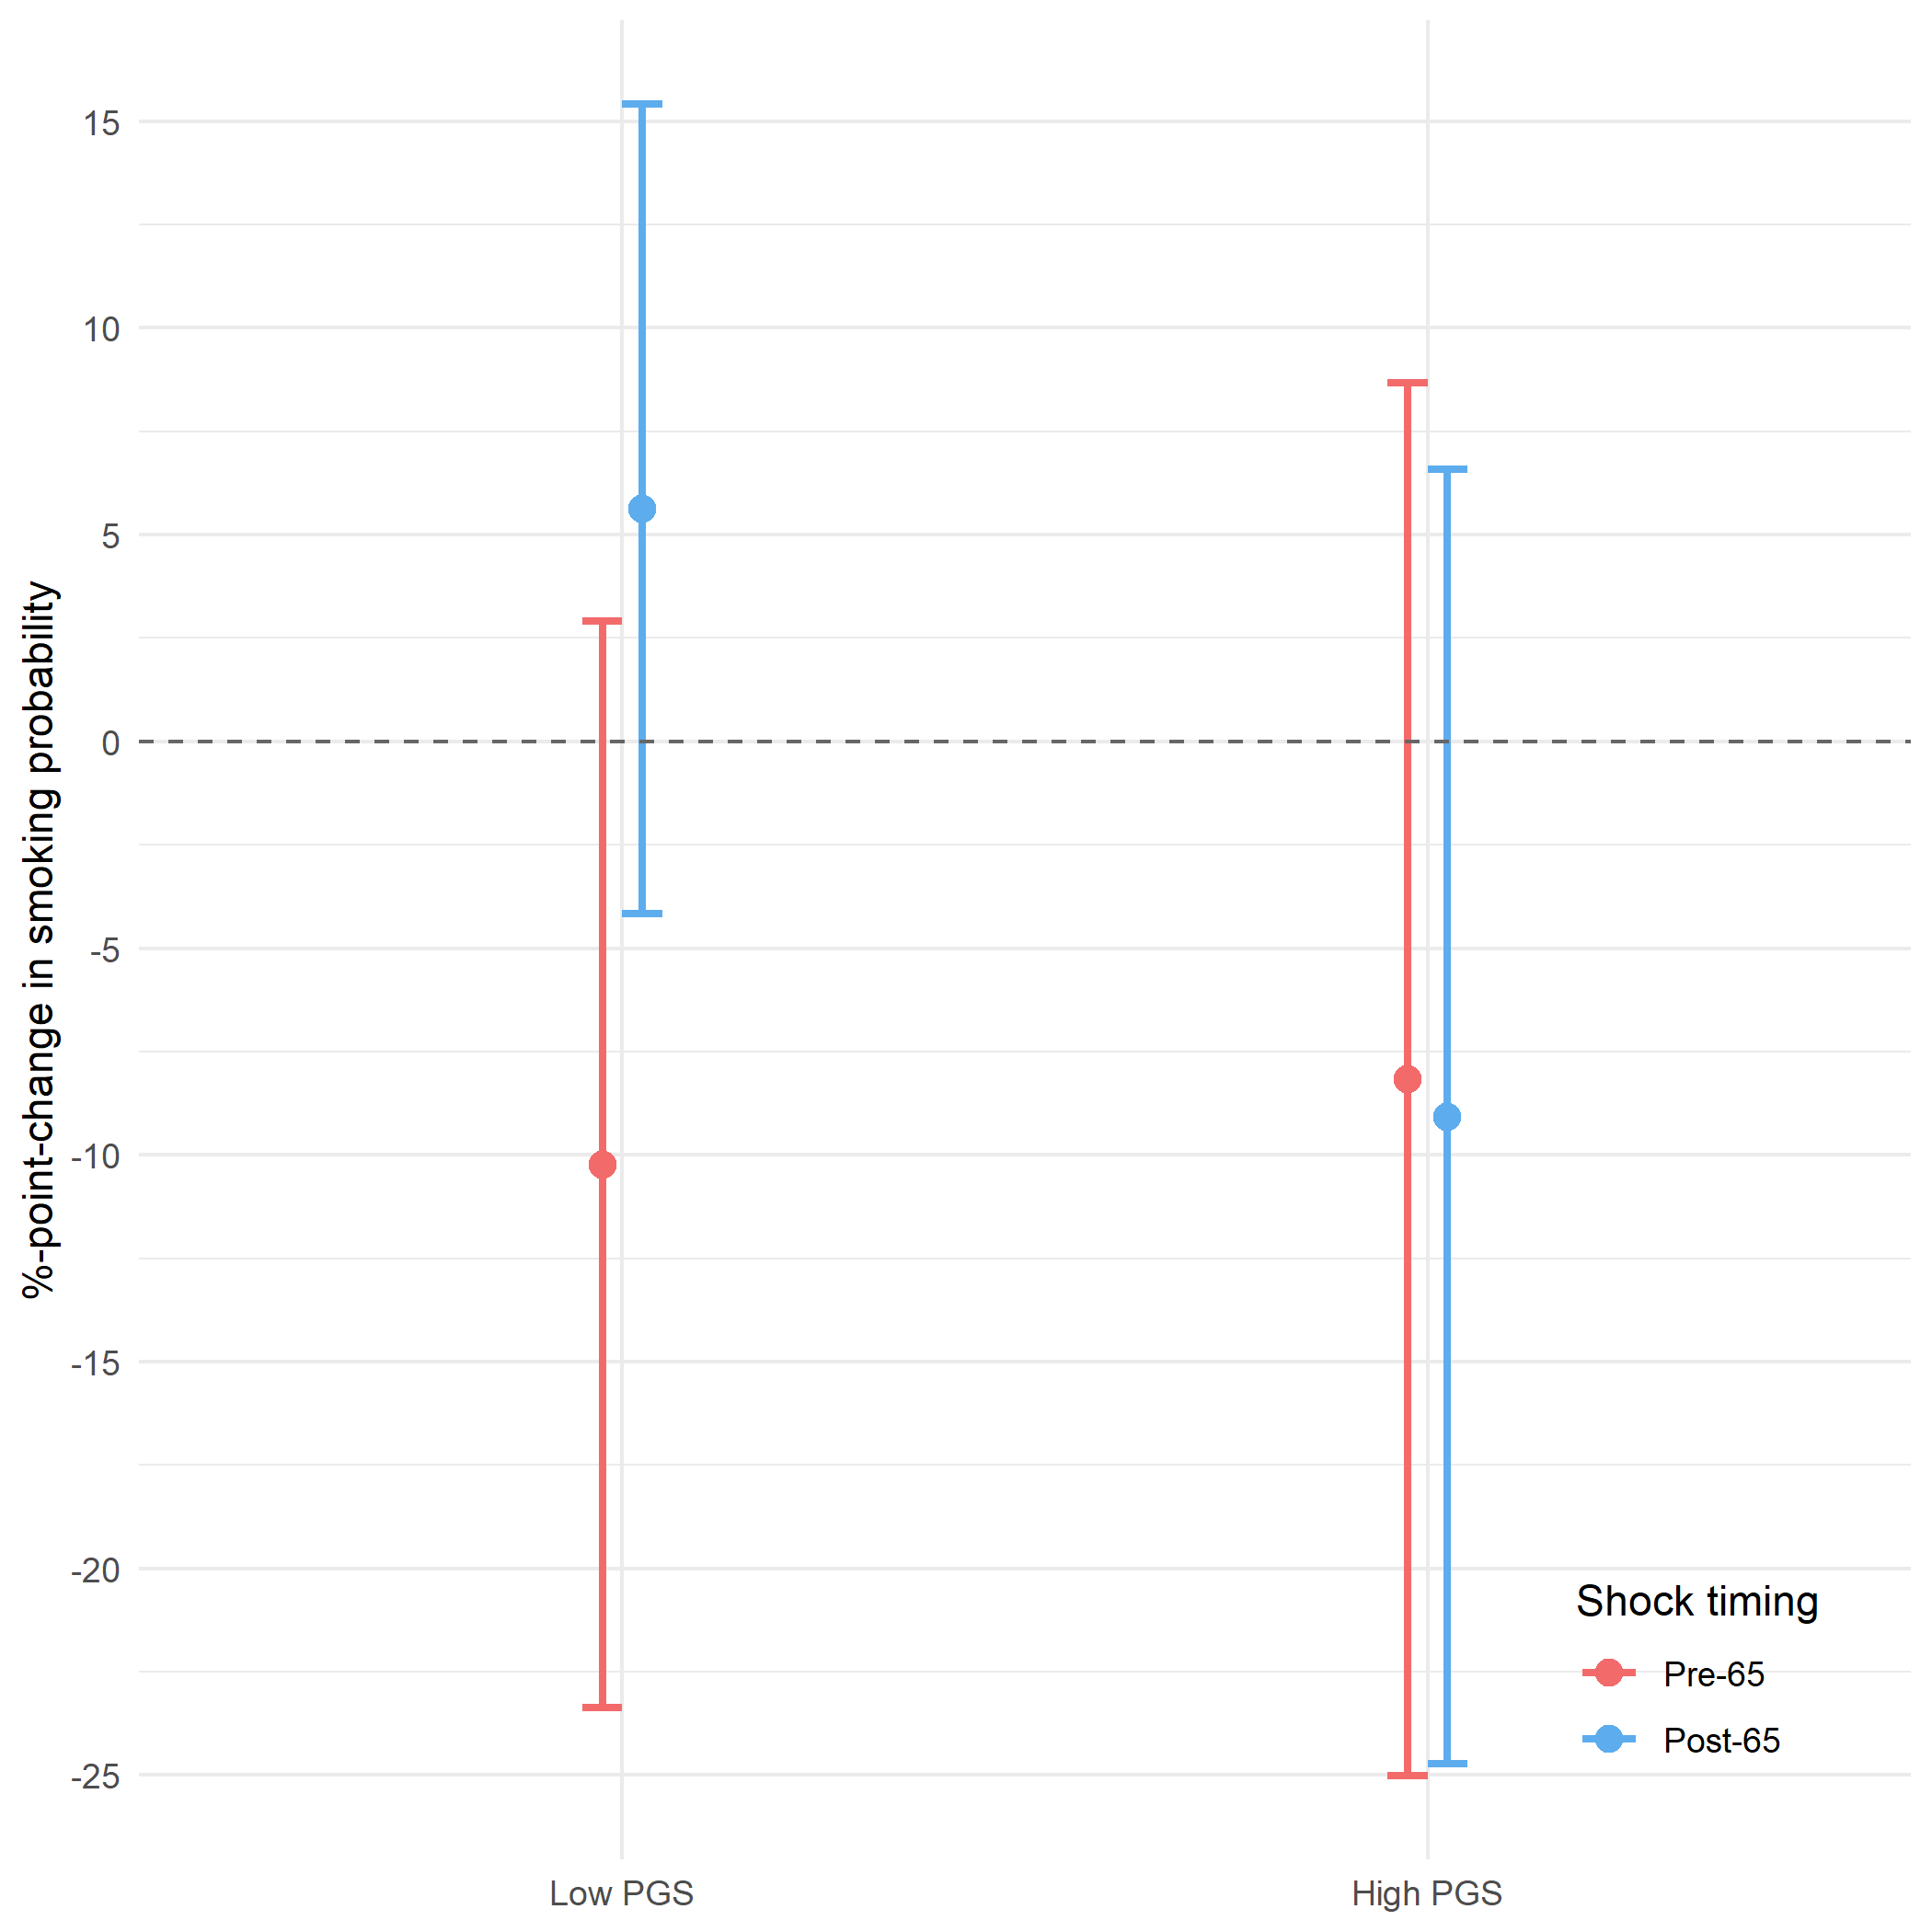
\includegraphics[height=0.8\textheight]{../../3_output/shock_effects/robustness_5971_100_cv.png}
\label{fig:coeffplot59-71}
\end{figure}
\hyperlink{frame:robustness}{\beamergotobutton{back}}
\end{frame}

%--------------------------------------------------------------%
\begin{frame}
\frametitle{Robustness: age range 58-72}
Coefficient plot of the main regression.
\begin{figure}[hbtp]

\centering
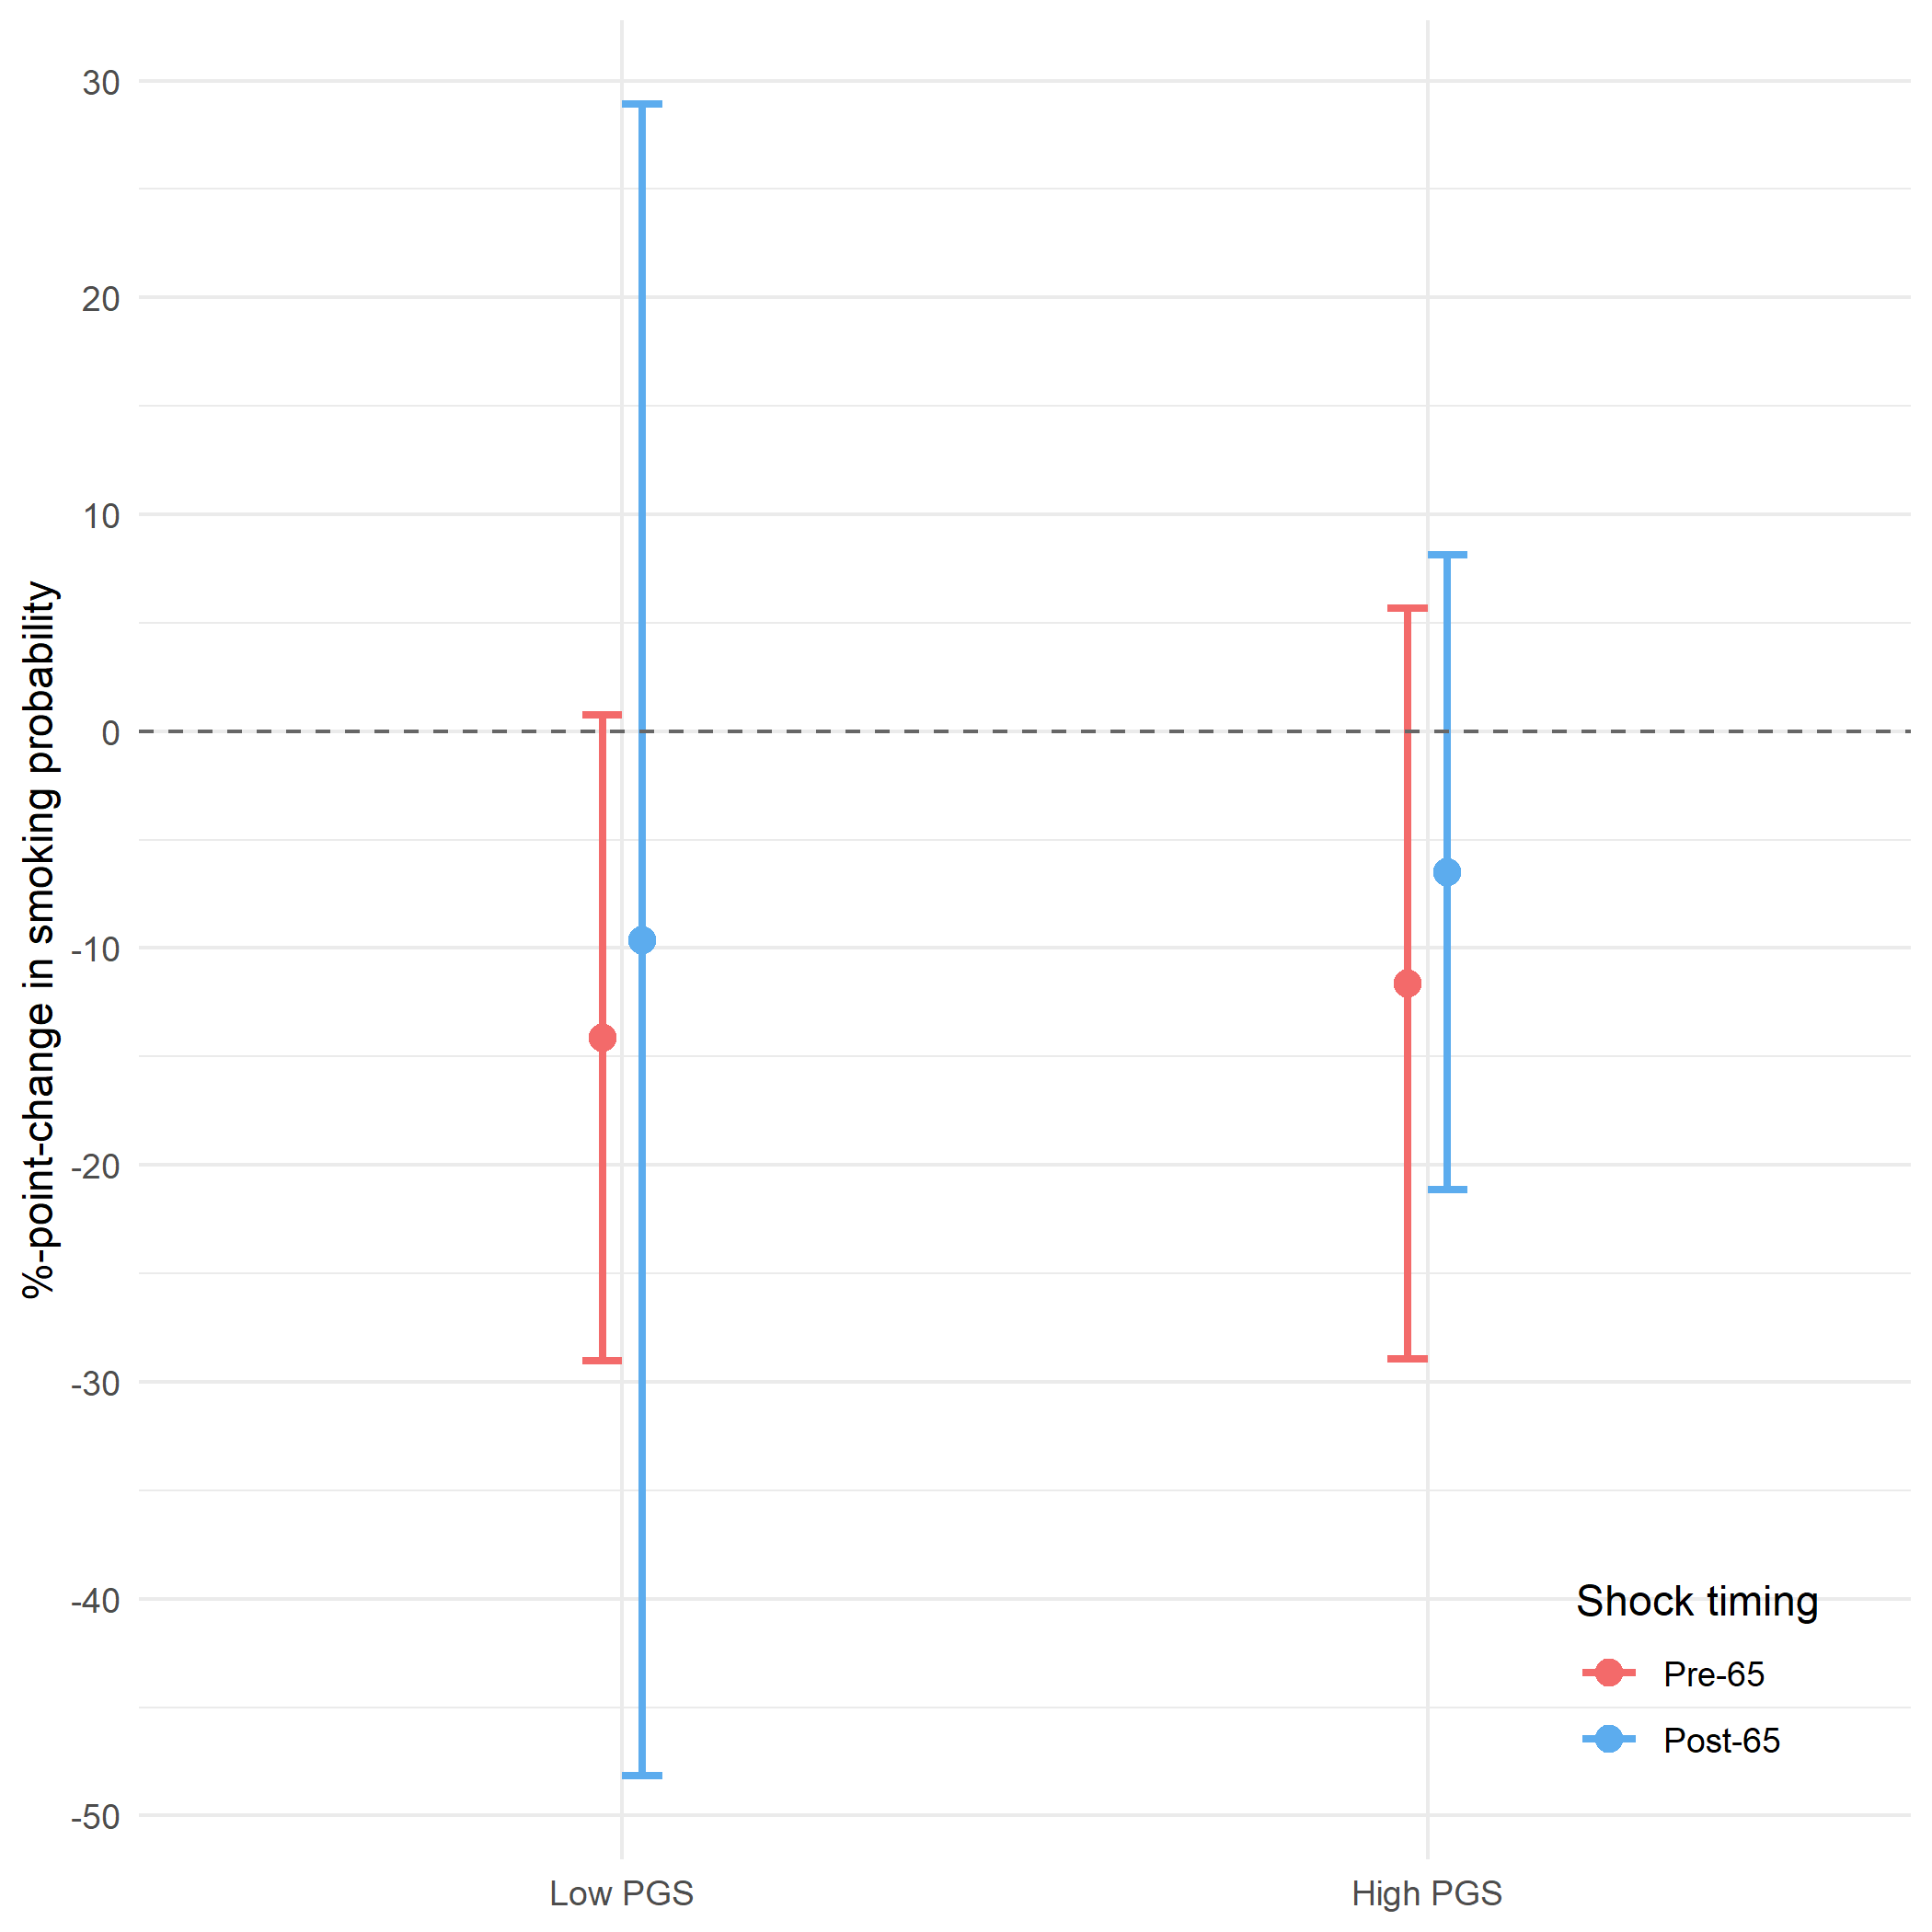
\includegraphics[height=0.8\textheight]{../../3_output/shock_effects/robustness_5872_100_cv.png}
\label{fig:coeffplot58-72}
\end{figure}
\hyperlink{frame:robustness}{\beamergotobutton{back}}
\end{frame}

%--------------------------------------------------------------%
\begin{frame}
\frametitle{Robustness: age range 55-70}
Coefficient plot of the main regression.
\begin{figure}[hbtp]

\centering
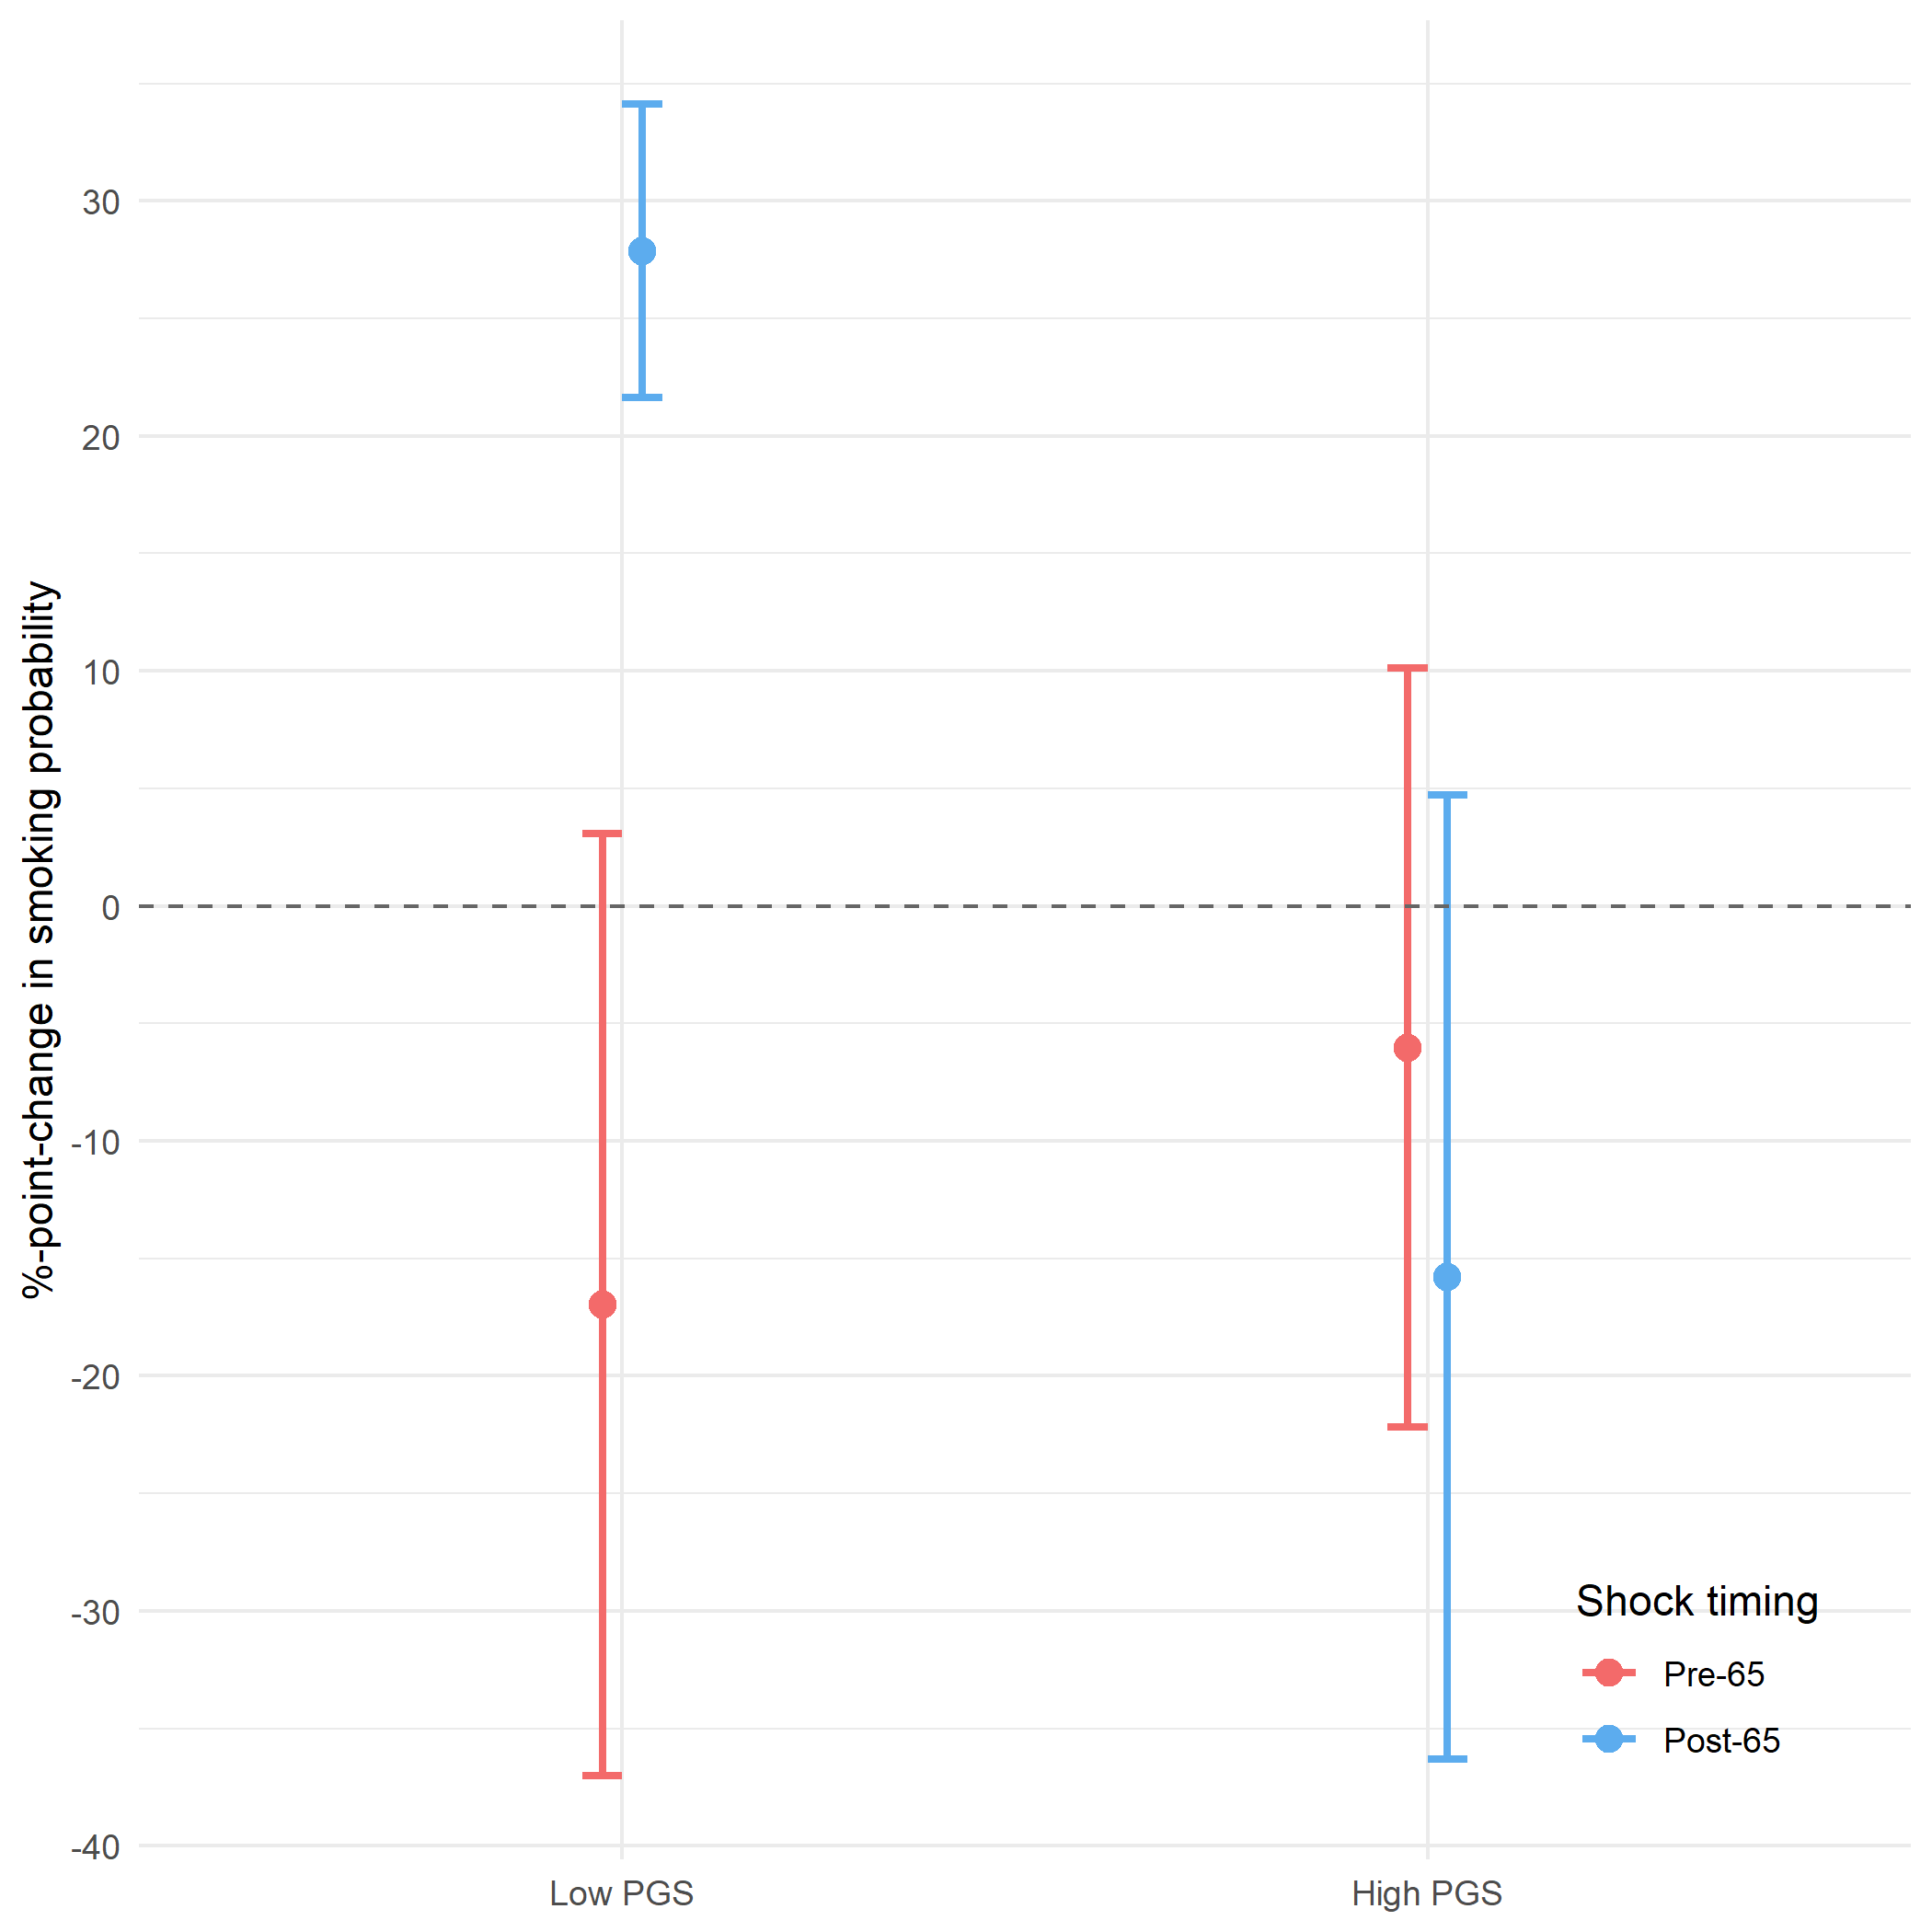
\includegraphics[height=0.8\textheight]{../../3_output/shock_effects/robustness_5570_100_cv.png}
\label{fig:coeffplot55-70}
\end{figure}
\hyperlink{frame:robustness}{\beamergotobutton{back}}
\end{frame}


%%--------------------------------------------------------------%
%\begin{frame}
%\frametitle{Robustness: age range 57-73}
%Coefficient plot of the main regression.
%\begin{figure}[hbtp]
%
%\centering
%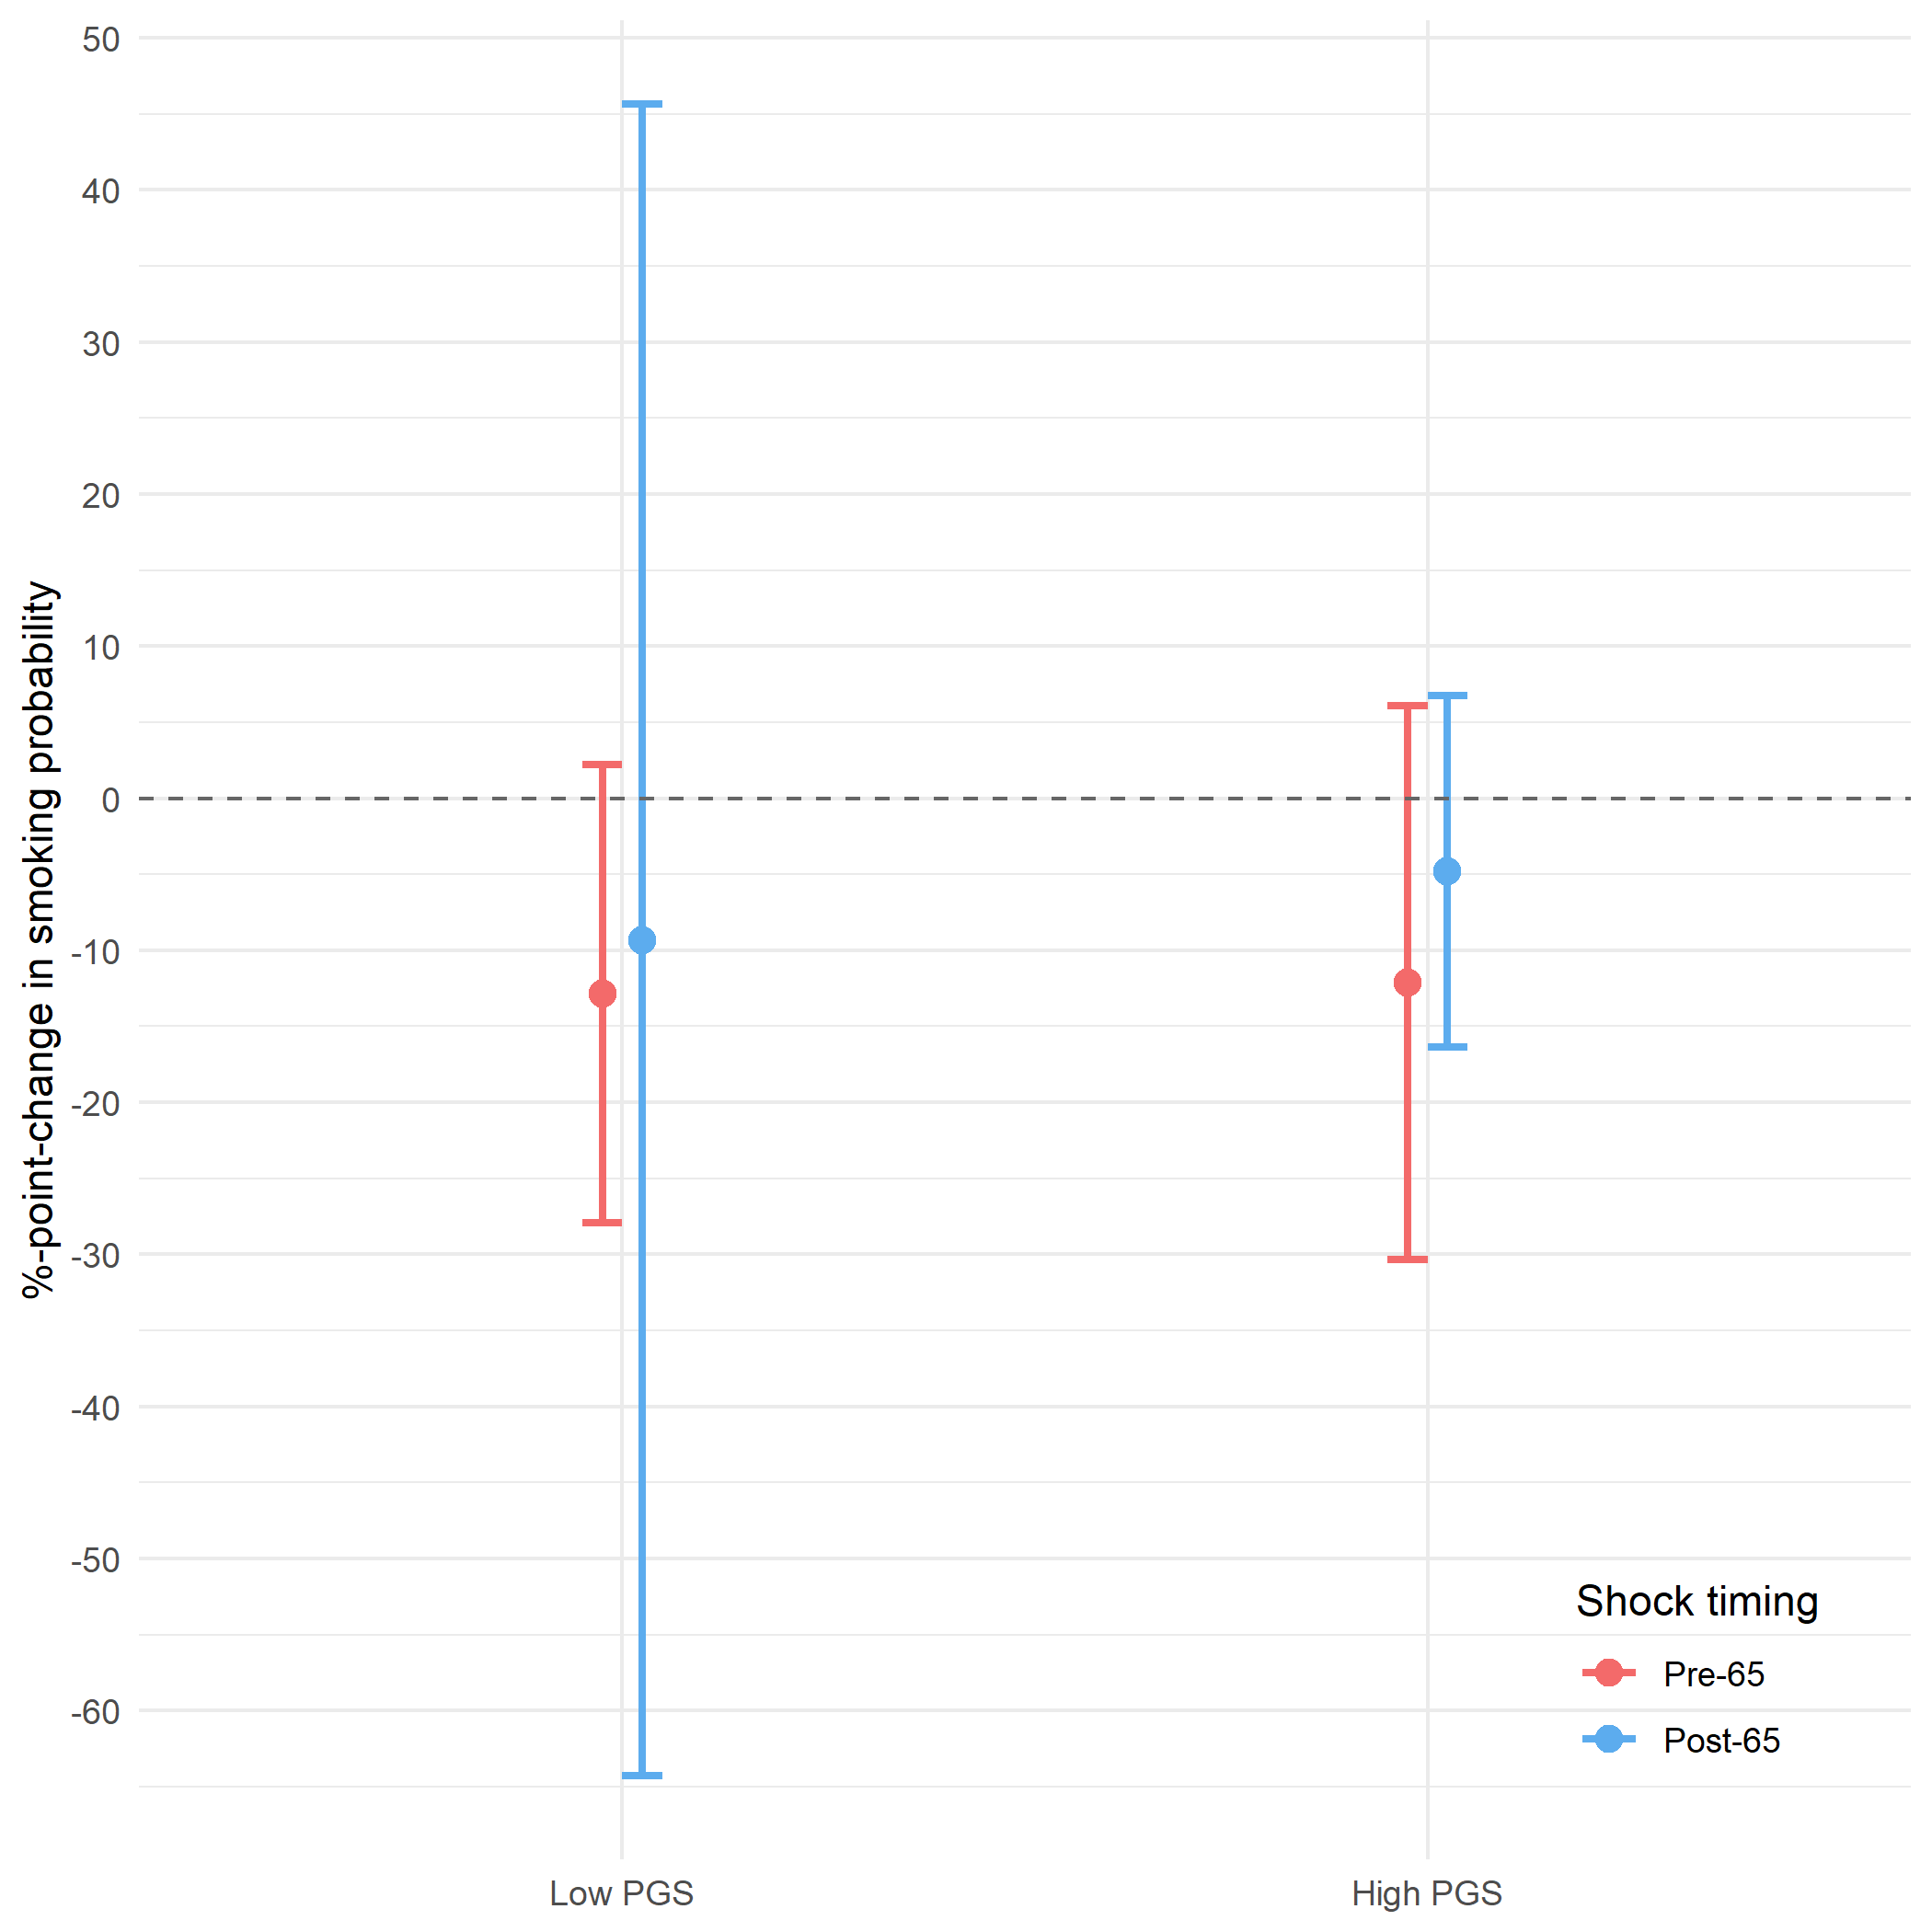
\includegraphics[height=0.8\textheight]{../../3_output/shock_effects/robustness_5773_100_cv.png}
%\label{fig:coeffplot57-73}
%\end{figure}
%\hyperlink{frame:robustness}{\beamergotobutton{back}}
%\end{frame}
%
%%--------------------------------------------------------------%
%\begin{frame}
%\frametitle{Robustness: age range 56-74}
%Coefficient plot of the main regression.
%\begin{figure}[hbtp]
%
%\centering
%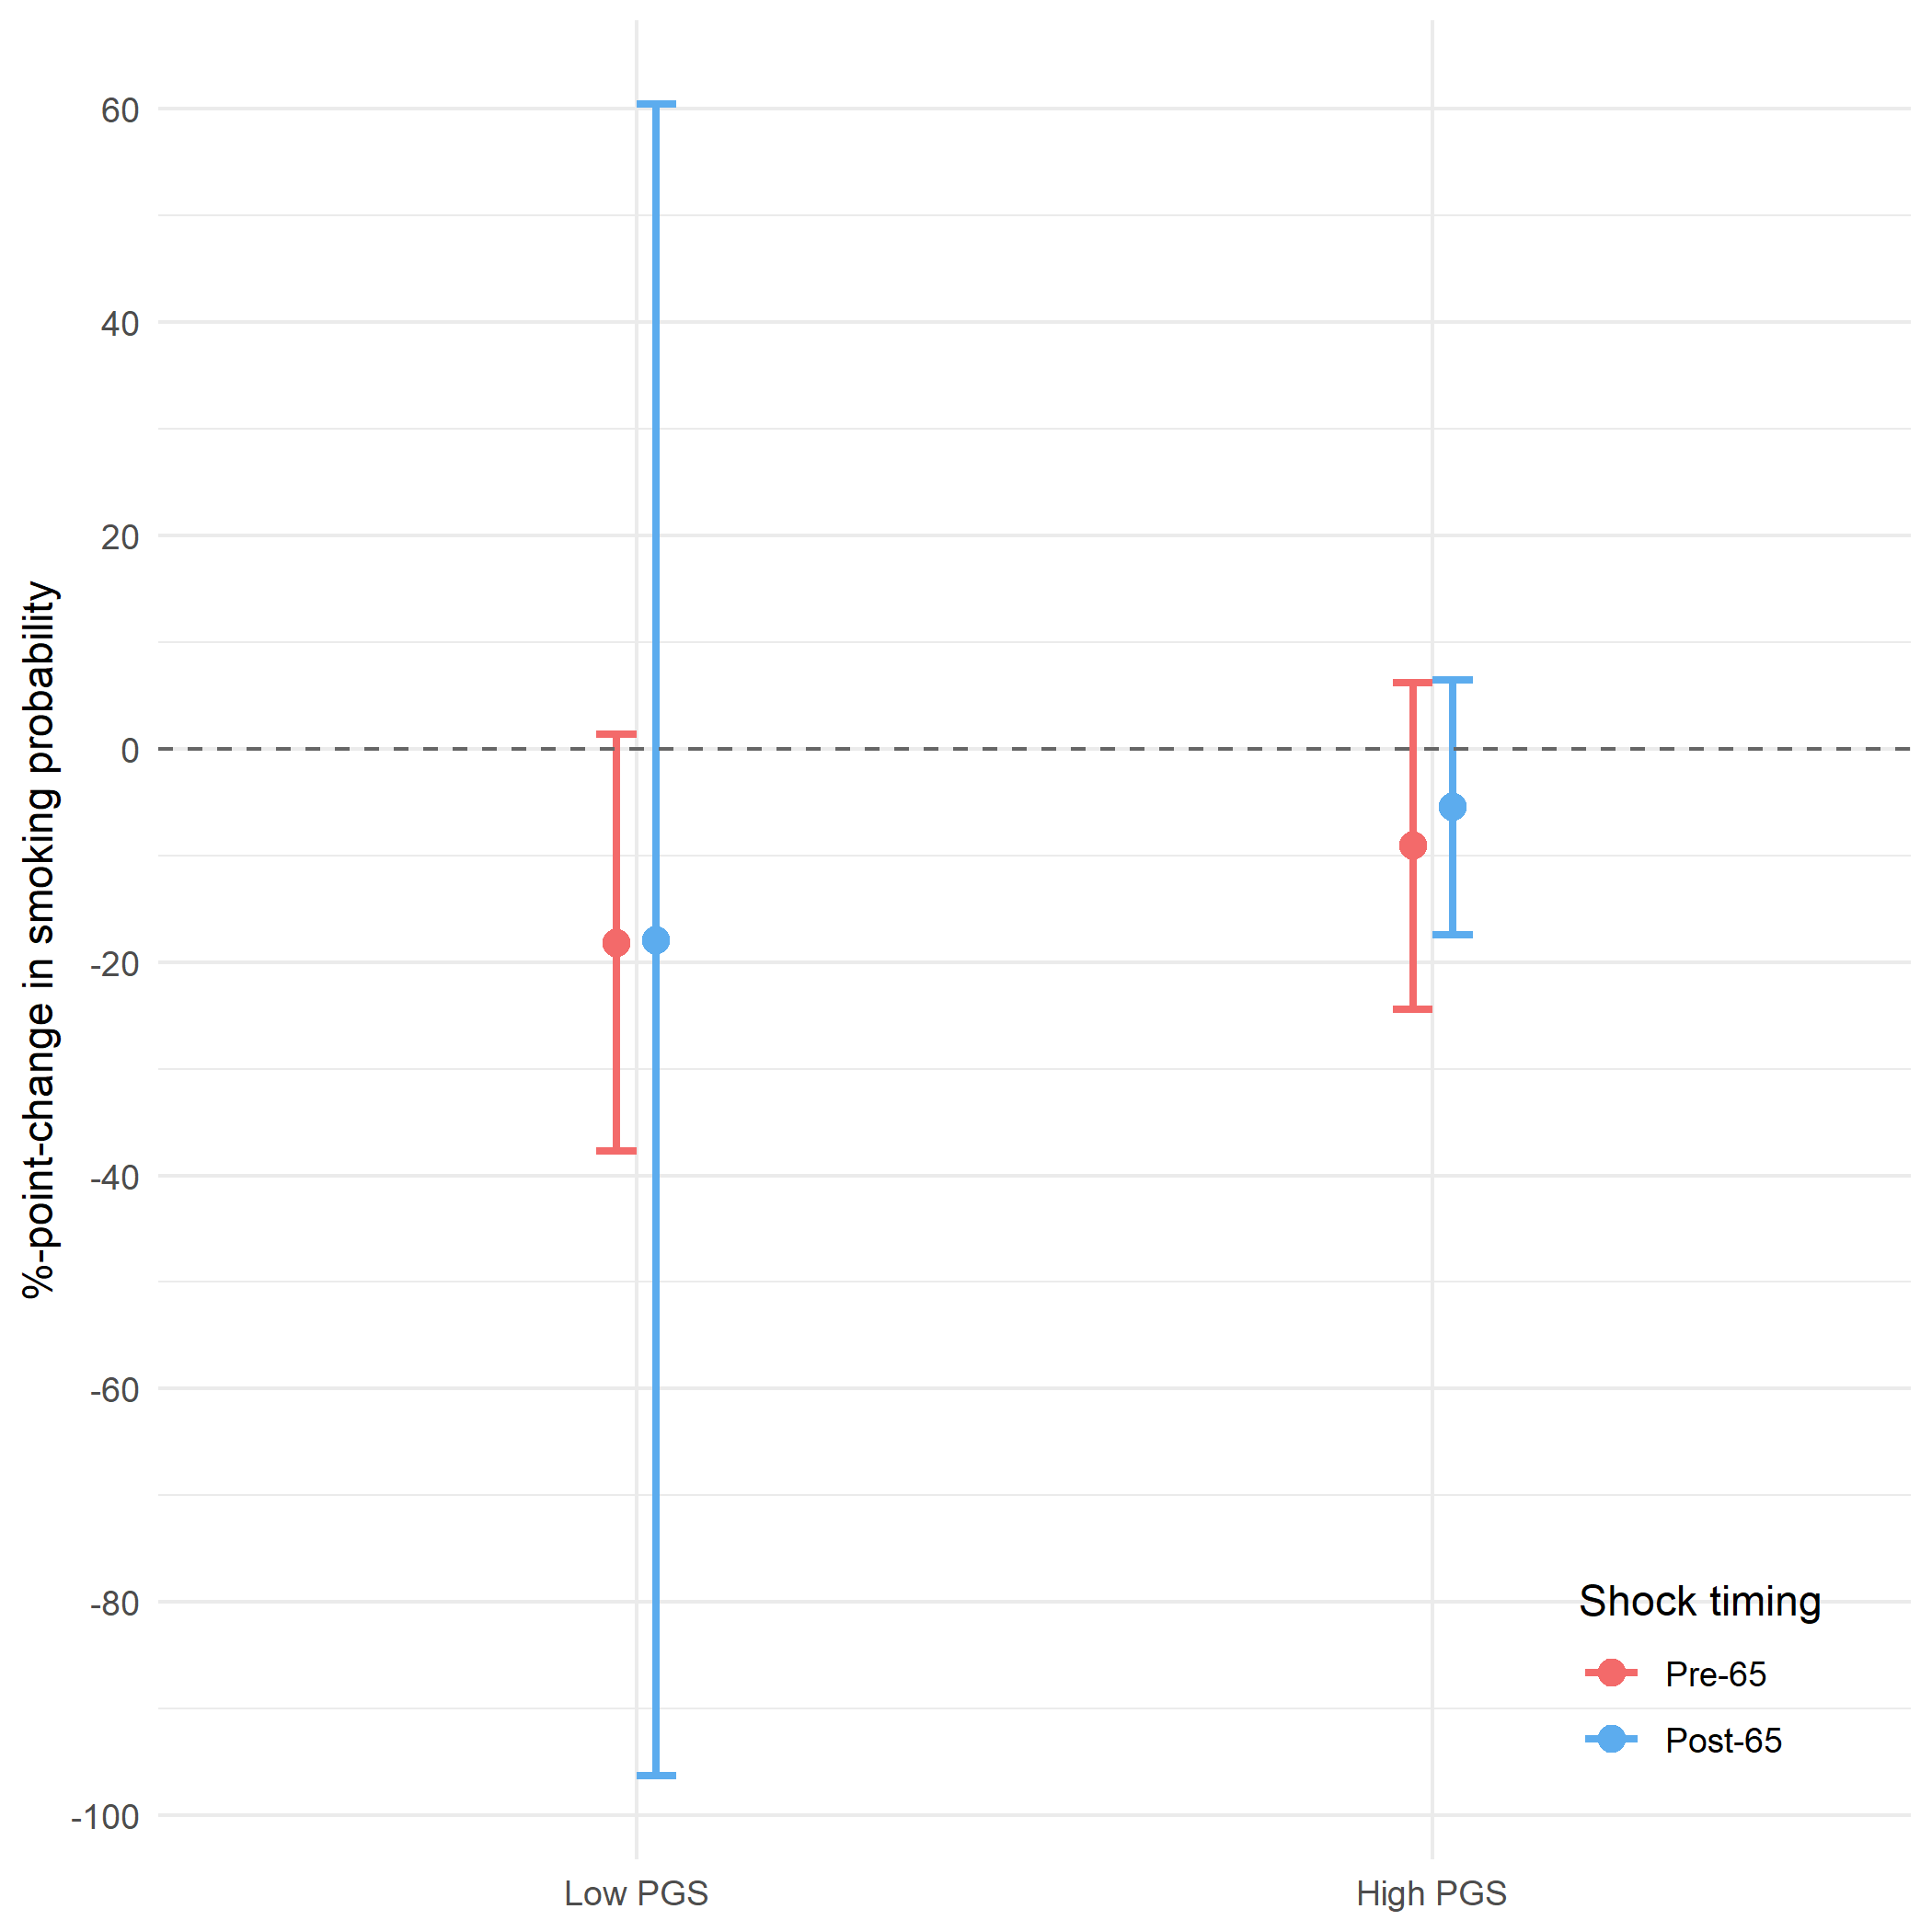
\includegraphics[height=0.8\textheight]{../../3_output/shock_effects/robustness_5674_100_cv.png}
%\label{fig:coeffplot56-74}
%\end{figure}
%\hyperlink{frame:robustness}{\beamergotobutton{back}}
%\end{frame}

\subsubsection{App: Robustness by uninsured spells}
%------------ ROBUSTNESS UNINSURED -----------------------------%
%--------------------------------------------------------------%
\begin{frame}
\frametitle{Robustness: uninsured only 2/3 of the time}
Coefficient plot of the main regression.
\begin{figure}[hbtp]

\centering
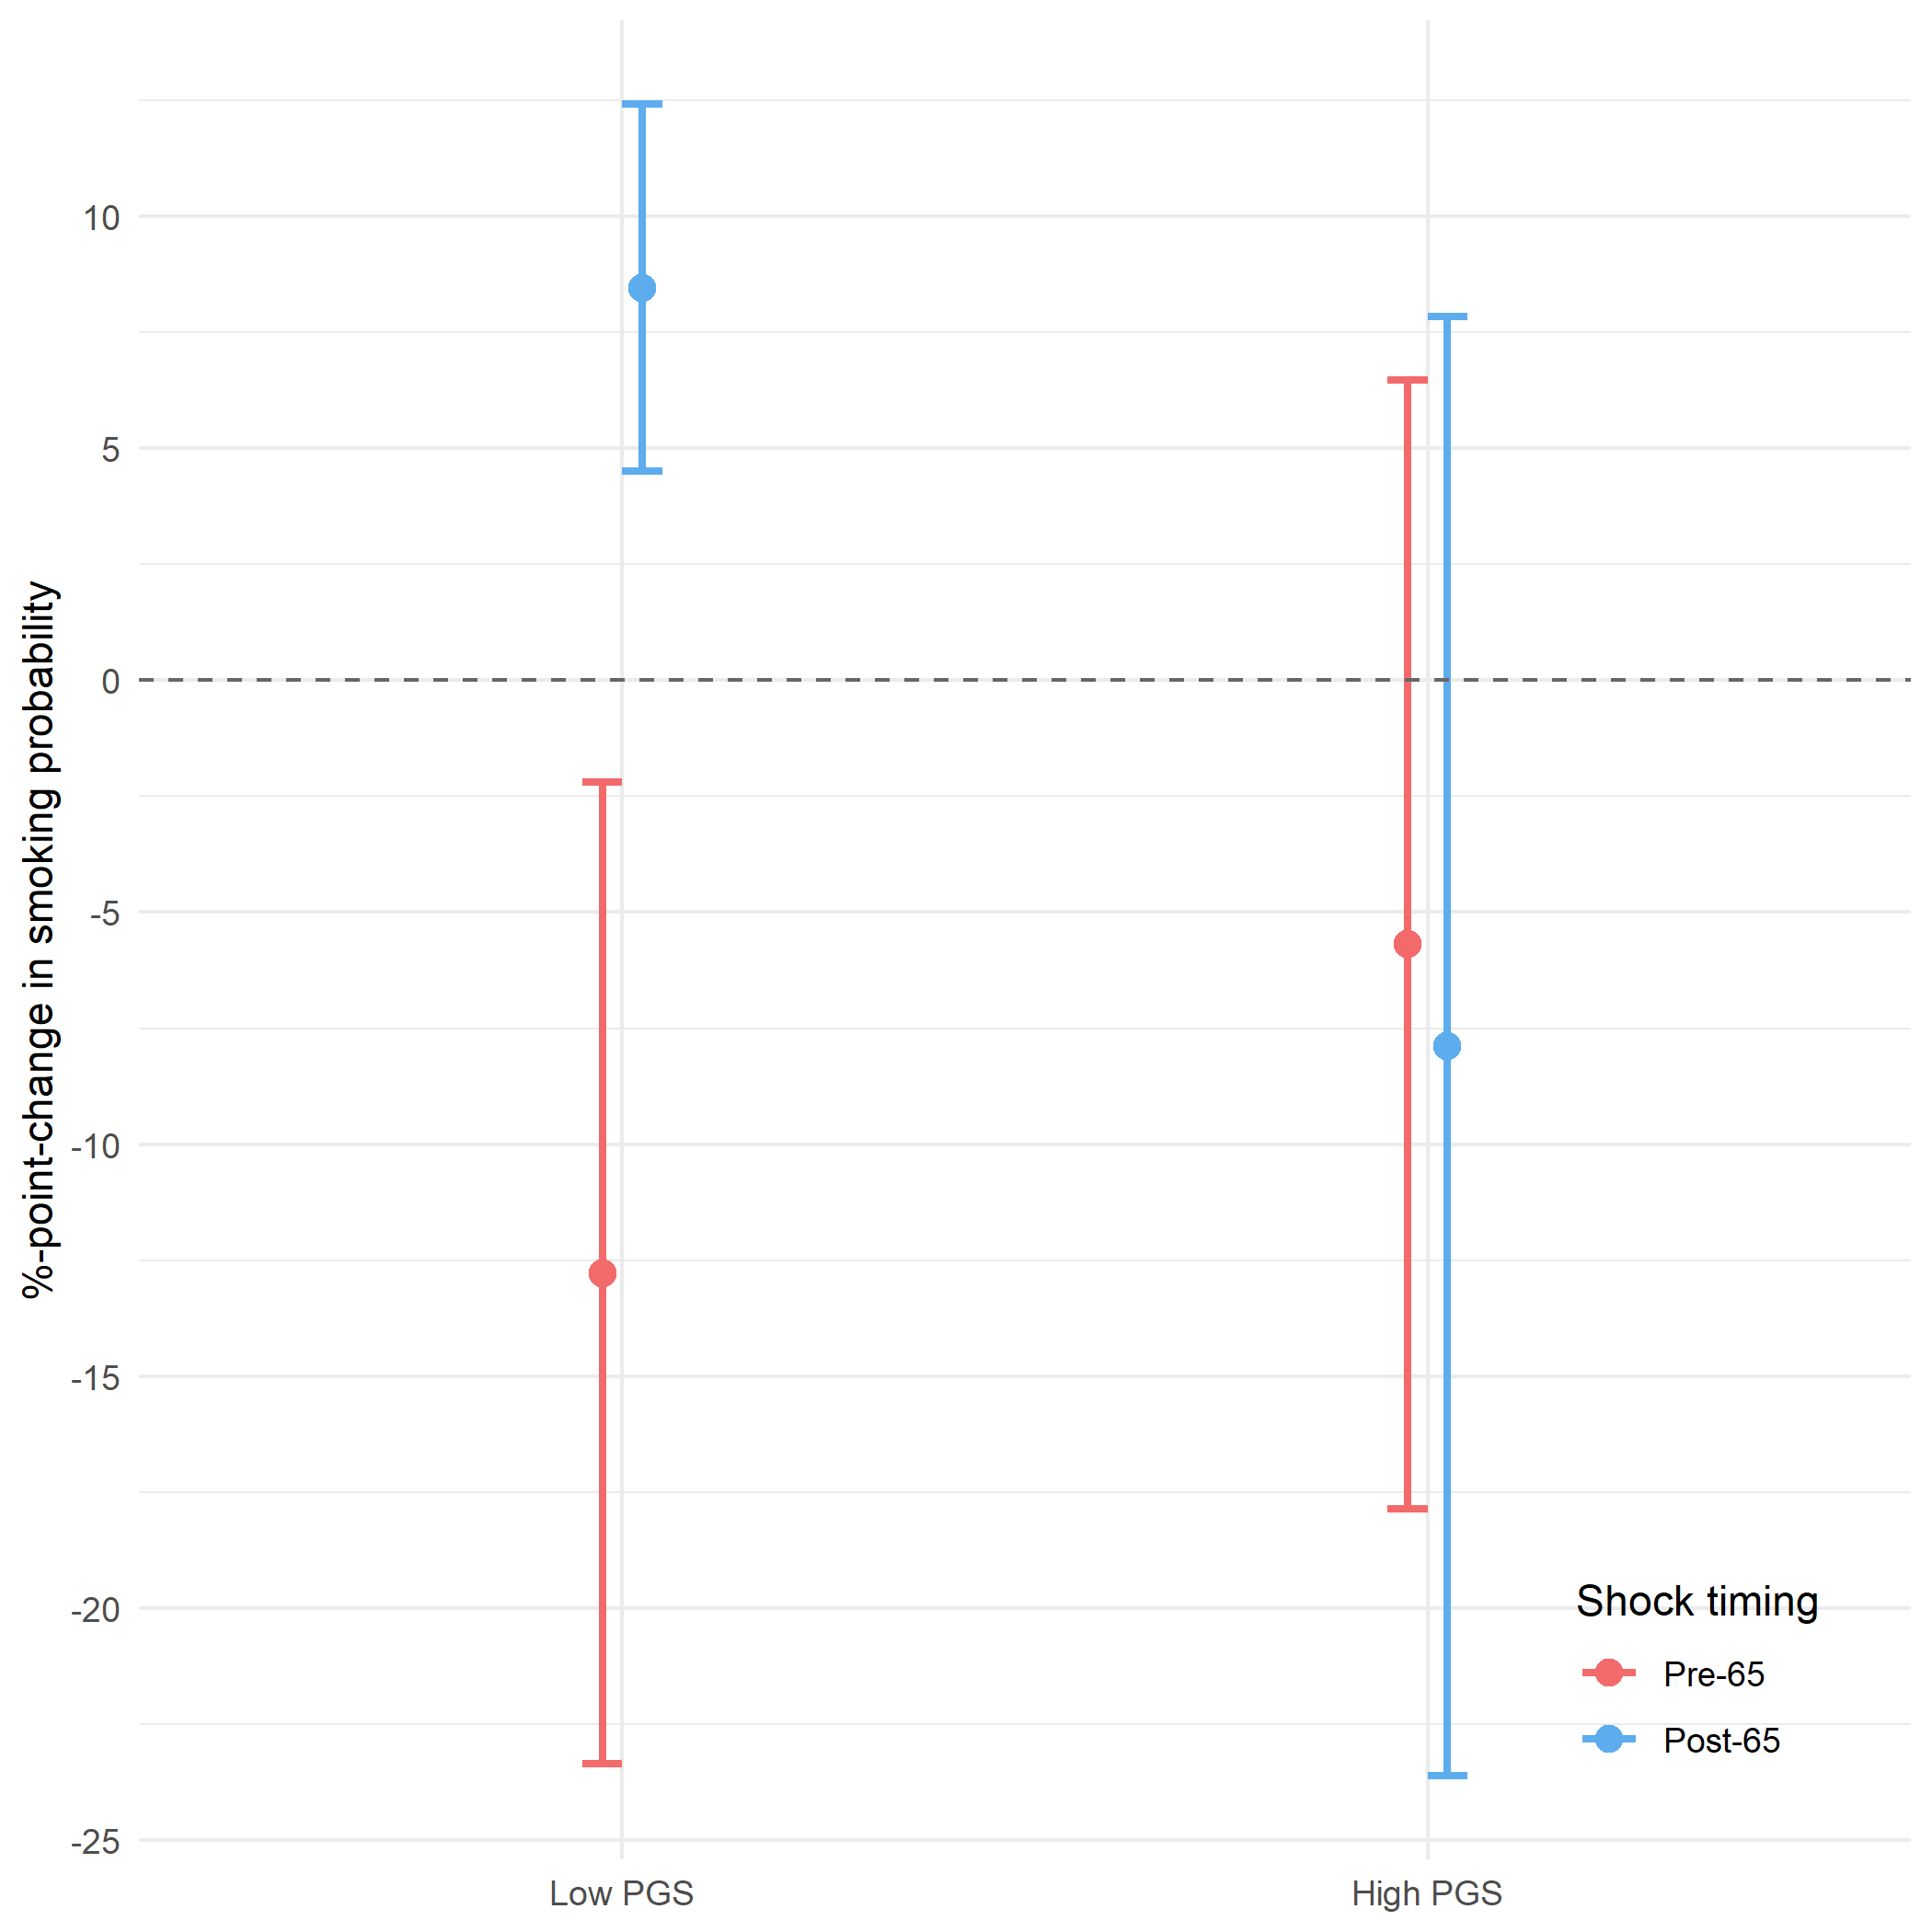
\includegraphics[height=0.8\textheight]{../../3_output/shock_effects/robustness_607066_cv.png}
\label{fig:coeffplot66unins}
\end{figure}
\hyperlink{frame:robustness}{\beamergotobutton{back}}
\end{frame}

%--------------------------------------------------------------%
\begin{frame}
\frametitle{Robustness: uninsured only 1/3 of the time}
Coefficient plot of the main regression.
\begin{figure}[hbtp]

\centering
\includegraphics[height=0.8\textheight]{../../3_output/shock_effects/robustness_607033_cv.png}
\label{fig:coeffplot33unins}
\end{figure}
\hyperlink{frame:robustness}{\beamergotobutton{back}}
\end{frame}

\subsubsection{App: Robustness by PGS cutoffs}
%------------ ROBUSTNESS PGS cutoff -----------------------------%
%%--------------------------------------------------------------%
%\begin{frame}
%\frametitle{Robustness: high PGS if above 75$^{th}$ percentile}
%Coefficient plot of the main regression.
%\begin{figure}[hbtp]
%
%\centering
%\includegraphics[height=0.8\textheight]{../../3_output/shock_effects/robustness_6070_100_cv_75p.png}
%\label{fig:coeffplot75highPGS}
%\end{figure}
%\hyperlink{frame:robustness}{\beamergotobutton{back}}
%\end{frame}
%
%%--------------------------------------------------------------%
%\begin{frame}
%\frametitle{Robustness: high PGS if above 25$^{th}$ percentile}
%Coefficient plot of the main regression.
%\begin{figure}[hbtp]
%
%\centering
%\includegraphics[height=0.8\textheight]{../../3_output/shock_effects/robustness_6070_100_cv_25p.png}
%\label{fig:coeffplot25highPGS}
%\end{figure}
%\hyperlink{frame:robustness}{\beamergotobutton{back}}
%\end{frame}
%

\subsubsection{App Robustness by other PGS}
%--------------------------------------------------------------%
\begin{frame}
\frametitle{Split by cognitive ability PGS}

\begin{figure}[hbtp]
\centering
\includegraphics[height=0.8\textheight]{../../3_output/shock_effects/robustness_cogPGS_6070_100_cv.png}
\label{fig:cogPGS}
\end{figure}
\hyperlink{frame:otherX}{\beamergotobutton{back}}
\end{frame}

%%--------------------------------------------------------------%
%\begin{frame}
%\frametitle{Split by non-cognitive ability PGS}
%
%\begin{figure}[hbtp]
%\centering
%\includegraphics[height=0.8\textheight]{../../3_output/shock_effects/robustness_noncogPGS_6070_100_cv.png}
%\label{fig:noncogPGS}
%\end{figure}
%\hyperlink{frame:otherX}{\beamergotobutton{back}}
%\end{frame}
%
%--------------------------------------------------------------%
\begin{frame}
\frametitle{Split by risk-seeking PGS}

\begin{figure}[hbtp]
\centering
\includegraphics[height=0.8\textheight]{../../3_output/shock_effects/robustness_riskPGS_GWAS_6070_100_cv.png}
\label{fig:riskPGS}
\end{figure}
\hyperlink{frame:otherX}{\beamergotobutton{back}}
\end{frame}

%%--------------------------------------------------------------%
%\begin{frame}
%\frametitle{Split by educational attainment PGS}
%
%\begin{figure}[hbtp]
%\centering
%\includegraphics[height=0.8\textheight]{../../3_output/shock_effects/robustness_ea3PGS_6070_100_cv.png}
%\label{fig:ea3PGS}
%\end{figure}
%\hyperlink{frame:otherX}{\beamergotobutton{back}}
%\end{frame}
%

\subsubsection{App: Potential mediators}
%%------------ POTENTIAL MEDIATORS -----------------------------%
%%--------------------------------------------------------------%
%\begin{frame}
%\frametitle{Retirement: not likely a Confounder}
%Coefficient plot of the main regression.
%\begin{figure}[hbtp]
%
%\centering
%\includegraphics[height=0.8\textheight]{../../3_output/shock_effects/retire_6070_100_cv.png}
%\label{fig:retire}
%\end{figure}
%\hyperlink{frame:robustness}{\beamergotobutton{back}}
%\end{frame}
%
%%--------------------------------------------------------------%
%\begin{frame}
%\frametitle{Wage: not likely a Confounder}
%Coefficient plot of the main regression.
%\begin{figure}[hbtp]
%
%\centering
%\includegraphics[height=0.8\textheight]{../../3_output/shock_effects/wage_6070_100_cv.png}
%\label{fig:wage}
%\end{figure}
%\hyperlink{frame:robustness}{\beamergotobutton{back}}
%\end{frame}

%--------------------------------------------------------------%
\begin{frame}\label{frame:dollargenome}
\frametitle{DNA Sequencing Cost}
Cost of sequencing the DNA has been falling rapidly (\href{https://www.genome.gov/about-genomics/fact-sheets/Sequencing-Human-Genome-cost}{NIH)}

\includegraphics[height=0.7\textheight]{./include/Sequencing_Cost_per_Genome_May2020.jpg}

\vspace{2ex}

Cost per participant: $\approx$ 50 \$ (with SNP imputation)

\hyperlink{frame:why}{\beamergotobutton{back}}

\end{frame}



%--------------------------------------------------------------%
\begin{frame}[allowframebreaks]
\frametitle{References}
\begin{tiny}
\bibliographystyle{apalike}
%\bibliography{C:/Users/pbiroli/Documents/Papers/library}  %from laptop
% source picture: https://ululalbab31n.blogspot.com/2017/01/single-nucleotide-polymorphism.html
\bibliography{../health_genes}
\end{tiny}
\end{frame}
%-%-%-%-%-%-%-%-%-%-%-%-%-%-%

\end{document}
